\documentclass[b5paper,openany]{ctexbook}
% openany 表示每一章第一页既可以在左也可以在右
\usepackage{geometry}
\geometry{
    top=2.25cm,
    bottom=2.25cm,
    inner=2cm, % left
    outer=2cm, % right
		headheight=5ex, % 页眉高度
		headsep=5ex, % 页眉和正文间距
}
\raggedbottom % 防止 vbox underfull 警告

\usepackage{fancyhdr} % 用来设置页眉页脚
\renewcommand{\sectionmark}[1]{\markright{\S\,\thesection\quad#1}}
% 正文格式
\fancypagestyle{fancy}{
  \fancyhf{} % 清除页眉页脚格式
  \fancyhead[LE,RO]{\thepage} % 页码显示
  \fancyhead[CE]{\leftmark} % 偶页页眉中心 
  \fancyhead[CO]{\rightmark} % 奇页页眉中心
}
% 目录第一页及 chapter 第一页格式
\fancypagestyle{plain}{\fancyhf{}}
% 目录与前言格式
\fancypagestyle{toc}{ 
  \fancyhf{}
  \fancyhead[LE,RO]{\thepage\vspace{1mm}}
}
\renewcommand{\headrulewidth}{0pt} % 去掉页眉横线

\pagestyle{plain}
\usepackage{float}
\usepackage{amssymb}
\usepackage{amsmath}
\usepackage{amsfonts}
\numberwithin{figure}{chapter}
\usepackage{graphicx}
\usepackage{enumerate} % 多种样式的 enumerate 编号
%\usepackage{enumitem} % 多种样式的 enumerate 编号
\usepackage{bm} %希腊字母加粗
\usepackage{xcolor} % \textcolor{red}{123}
\usepackage{amsthm}
% 让定理的标题变为粗体
\makeatletter
\def\th@plain{%
  \thm@notefont{}% same as heading font
  \itshape % body font
}
\def\th@definition{%
  \thm@notefont{}% same as heading font
  \normalfont % body font
}
\makeatother
\newtheorem{theorem}{定理}[chapter]
\newtheorem{axiom}[theorem]{公理}
\newtheorem{lemma}[theorem]{引理}
\newtheorem{definition}[theorem]{定义} 
\newtheorem{proposition}[theorem]{命题}
\newtheorem{corollary}[theorem]{推论}
\newtheorem{example}[theorem]{例}
\newtheorem*{remark}{注}

\newtheorem{quantumaxiom}{量子力学公理}

\usepackage{hyperref} % 文档内跳转
\usepackage{xpatch}
% 去掉定理编号后面的点
%\makeatletter
%\AtBeginDocument{\xpatchcmd{\@thm}{\thm@headpunct{.}}{\thm@headpunct{}}{}{}}
%\makeatother

% 证明粗体
\xpatchcmd{\proof}{\itshape}{\normalfont\proofnamefont}{}{}
\newcommand{\proofnamefont}{\bfseries}
% 提升 chi 的高度
\usepackage{mathtools}
\DeclareRobustCommand{\rchi}{{\mathpalette\irchi\relax}}
\newcommand{\irchi}[2]{\raisebox{\depth}{$#1\chi$}}
% 优化 forall 和 exists 后面的缩进
\let\oldforall\forall
\let\forall\undefined
\DeclareMathOperator{\forall}{\oldforall}
\let\oldexists\exists
\let\exists\undefined
\DeclareMathOperator{\exists}{\oldexists}

\usepackage{indentfirst}
\setlength{\parindent}{2em} %首行缩进
\usepackage{setspace} % 调整行间距
% 用来调整行间距, 不要与 setspace 混用
% \renewcommand{\baselinestretch}{1.25} 

% \keepline 可以用来让以行间公式开头的定理或证明不另起一行
% 使用方法:
% \begin{theorem}[title]\keepline
% ...
% \end{theorem}
\newcommand{\keepline}{\leavevmode\setlength{\abovedisplayskip}{0pt}\vspace{-\baselineskip}}
\usepackage{tikz}
\usepackage{pgfplots}
\pgfplotsset{compat=1.18}
\usepackage{epigraph}
\setlength\epigraphwidth{.7\textwidth}
% \renewcommand{\textflush}{flushright}
\setlength{\epigraphrule}{0pt}

\title{我的物理笔记}
\author{周子涵}
\date{\today}
\begin{document}
\maketitle
% 调整上下角标高度
\fontdimen17\textfont2=2.5pt 
\fontdimen16\textfont2=2.5pt
\fontdimen15\textfont2=4.5pt
\fontdimen14\textfont2=4.5pt
\fontdimen13\textfont2=4.5pt

\vspace*{7cm}
\begin{center}
    {\large 献给刘昱伯, 感谢他在我学习物理时所给予的帮助.}
\end{center}
\frontmatter
\pagestyle{toc} % 目录和前言页眉只有罗马数字页码
\include{sec/preface}
\tableofcontents
\pagestyle{plain} % 防止空白页出现页码
% \cleardoublepage
\mainmatter
\pagestyle{fancy} % 正文页眉格式
% \part{四大力学}
\chapter{经典力学}
本章主要介绍拉格朗日力学和哈密顿力学, 它们都是经典力学的重新表述, 与牛顿力学等价, 前者由拉格朗日于 1788 创立, 后者由哈密顿于 1833 年创立. 重新表述经典力学这件事本身不是最重要的, 最重要的是这两种框架非常强力, 因而被广泛使用于后续的物理中. 可以说, 想要学物理, 就必须先了解它们.

牛顿力学以 $ F=ma $ 及受力分析的方法为公理, 虽然``力''这个概念易于理解, 但实际操作起来麻烦, 在对比较复杂的系统作受力分析时要处处小心. 实际上, 力 (force) 这个概念是多余的, 我们完全可以绕过它来建立力学 (mechanics).

\section{拉格朗日力学}
在拉格朗日力学中, 真正重要的概念只有拉格朗日量和最小作用量原理, 其余所有东西都可以由它们推出.

考虑 $ \mathbb{R}^n $ 中若干个质点组成的系统, 其所有 (在约束下) 可能状态的全体构成了\textbf{位形空间} (configuration space). 能用来唯一地表示位形空间中的点的一组参数 $ q=(q^1,\dots,q^k) $ 叫做\textbf{广义坐标}, 其中的 $ k $ 叫做系统的\textbf{自由度}. 

系统状态随时间的演化构成了位形空间中的一条曲线 $ \gamma(t) $, 它的广义坐标 $ q(t)=(q_1(t),\dots,q_k(t)) $ 关于时间 $ t $ 的导数 $ \dot{q}(t) $ 叫做\textbf{广义速度}.
\begin{definition}[拉格朗日量]
    给定势能 $ V $, 则其对应的{\bf 拉格朗日量} (Lagrangian) 为函数 $ L(q,\dot{q},t):=T-V $, 其中 $ q $ 是广义坐标, $ \dot{q} $ 是广义速度, $ T $ 是动能, $ V $ 是势能.
\end{definition}
本书只考虑最简单的情况: 质量为 $ m $ 的质点的{\bf 动能}
\[ T=\frac{1}{2}m\dot{q}^2, \] 
对于多个质点构成的系统, 其动能为所有质点的动能之和; {\bf 势能} $ V $ 是位形空间上的函数. 此时 $ L $ 不显含时间变量 $ t $, 可将其记为 $ L(q,\dot{q}) $.

\begin{definition}[作用量]
    给定 $ [t_1,t_2]\subset\mathbb{R} $, 则{\bf 作用量} (action) 为泛函
    \[ S[q] :=\int_{t_1}^{t_2}L(q(t),\dot{q}(t),t)\,\mathrm{d}t.\]
\end{definition}

对于泛函 $ I(q) $, 固定 $ q=q_0 $, 若有 $ I(q_0+h)-I(q_0)=A(h)+R(q_0,h) $, 其中 $ A $ 关于 $ h $ 是线性的, 且 $ R(q_0,h)=o(h) $, 则称 $ I $ 是可微的, 称 $ A $ 为 $ I $ 在 $ q_0 $ 处的微分 (Fr\'{e}chet 导数). 泛函的微分又叫做变分, 记作 $ \delta I $.

\begin{axiom}[最小作用量原理]
    固定 $ q(t_1) $ 和 $ q(t_2) $, 则时间段 $ [t_1,t_2] $ 上的真实物理过程是满足 $ \delta S=0 $ 的 $ q(t) $.
\end{axiom}
\begin{remark}
    最小作用量原理也叫哈密顿原理. 
\end{remark}
\begin{theorem}[拉格朗日方程]
    最小作用量原理等价于{\bf 拉格朗日方程}
    \[ \frac{\partial L}{\partial q}-\frac{\mathrm{d}}{\mathrm{d}t}\frac{\partial L}{\partial\dot{q}}=0. \]
\end{theorem}
\begin{proof}
对于 $ S $, 有
\begin{align*}
    S[q+h]-S[q] &= \int_{t_1}^{t_2}\left[ L(q+h,\dot{q}+\dot{h},t)-L(q,\dot{q},t) \right]\mathrm{d}t\\ 
    &=\int_{t_1}^{t_2}\left[ \frac{\partial L}{\partial q}h+\frac{\partial L}{\partial\dot{q}}\dot{h} \right]\mathrm{d}t+o(h).
\end{align*}
由于 $ q(t_1) $ 和 $ q(t_2) $ 被固定了, 有 $ h(t_1)=h(t_2)=0 $. 由分部积分可得
\begin{align*}
    \int_{t_1}^{t_2}\frac{\partial L}{\partial\dot{q}}\dot{h}\,\mathrm{d}t &= \left.h\frac{\partial L}{\partial\dot{q}}\right|_{t_1}^{t_2}-\int_{t_1}^{t_2}h\frac{\mathrm{d}}{\mathrm{d}t}\left( \frac{\partial L}{\partial\dot{q}} \right)\mathrm{d}t\\ 
    &=-\int_{t_1}^{t_2}h\frac{\mathrm{d}}{\mathrm{d}t}\left( \frac{\partial L}{\partial\dot{q}} \right)\mathrm{d}t.
\end{align*}
综上有
\[ S[q+h]-S[q]=\int_{t_1}^{t_2}\left[ \frac{\partial L}{\partial q}-\frac{\mathrm{d}}{\mathrm{d}t}\frac{\partial L}{\partial\dot{q}} \right] h\,\mathrm{d}t + o(h). \]

根据定义, $ S $ 在 $ q $ 处的变分为
\[ \delta S[q](h) = \int_{t_1}^{t_2}\left[ \frac{\partial L}{\partial q}-\frac{\mathrm{d}}{\mathrm{d}t}\frac{\partial L}{\partial\dot{q}} \right] h\,\mathrm{d}t, \]
因此 $ \delta S=0 $ 等价于 
\[ \frac{\partial L}{\partial q}-\frac{\mathrm{d}}{\mathrm{d}t}\frac{\partial L}{\partial\dot{q}}=0. \qedhere\]
\end{proof}

若定义广义动量 $p$ 和广义力 $F$ 为
\[ p:=\frac{\partial L}{\partial\dot{q}},\quad F:=\frac{\partial L}{\partial q}, \] 
则拉格朗日方程可表达为 $ F=\dot{p} $, 与 $F=ma$ 形式一致. 在牛顿力学中, 我们先做受力分析, 然后解 $ F=ma $, 从而得到质点的运动轨迹; 在拉格朗日力学中, 我们先写出拉格朗日量, 然后解拉格朗日方程, 从而得到 $ q(t) $.

与牛顿力学相比, 拉格朗日力学的优势在于不需要做繁琐的受力分析, 更适合处理复杂系统. 我们可以从下面这个经典例子中一窥拉格朗日力学的优雅.

\begin{example}[双摆]
    如图 \ref{double pendulum} 所示, 假设两小球为质点, 连接他们的杆是无质量刚体. 
    \begin{figure}[H]
        \centering
        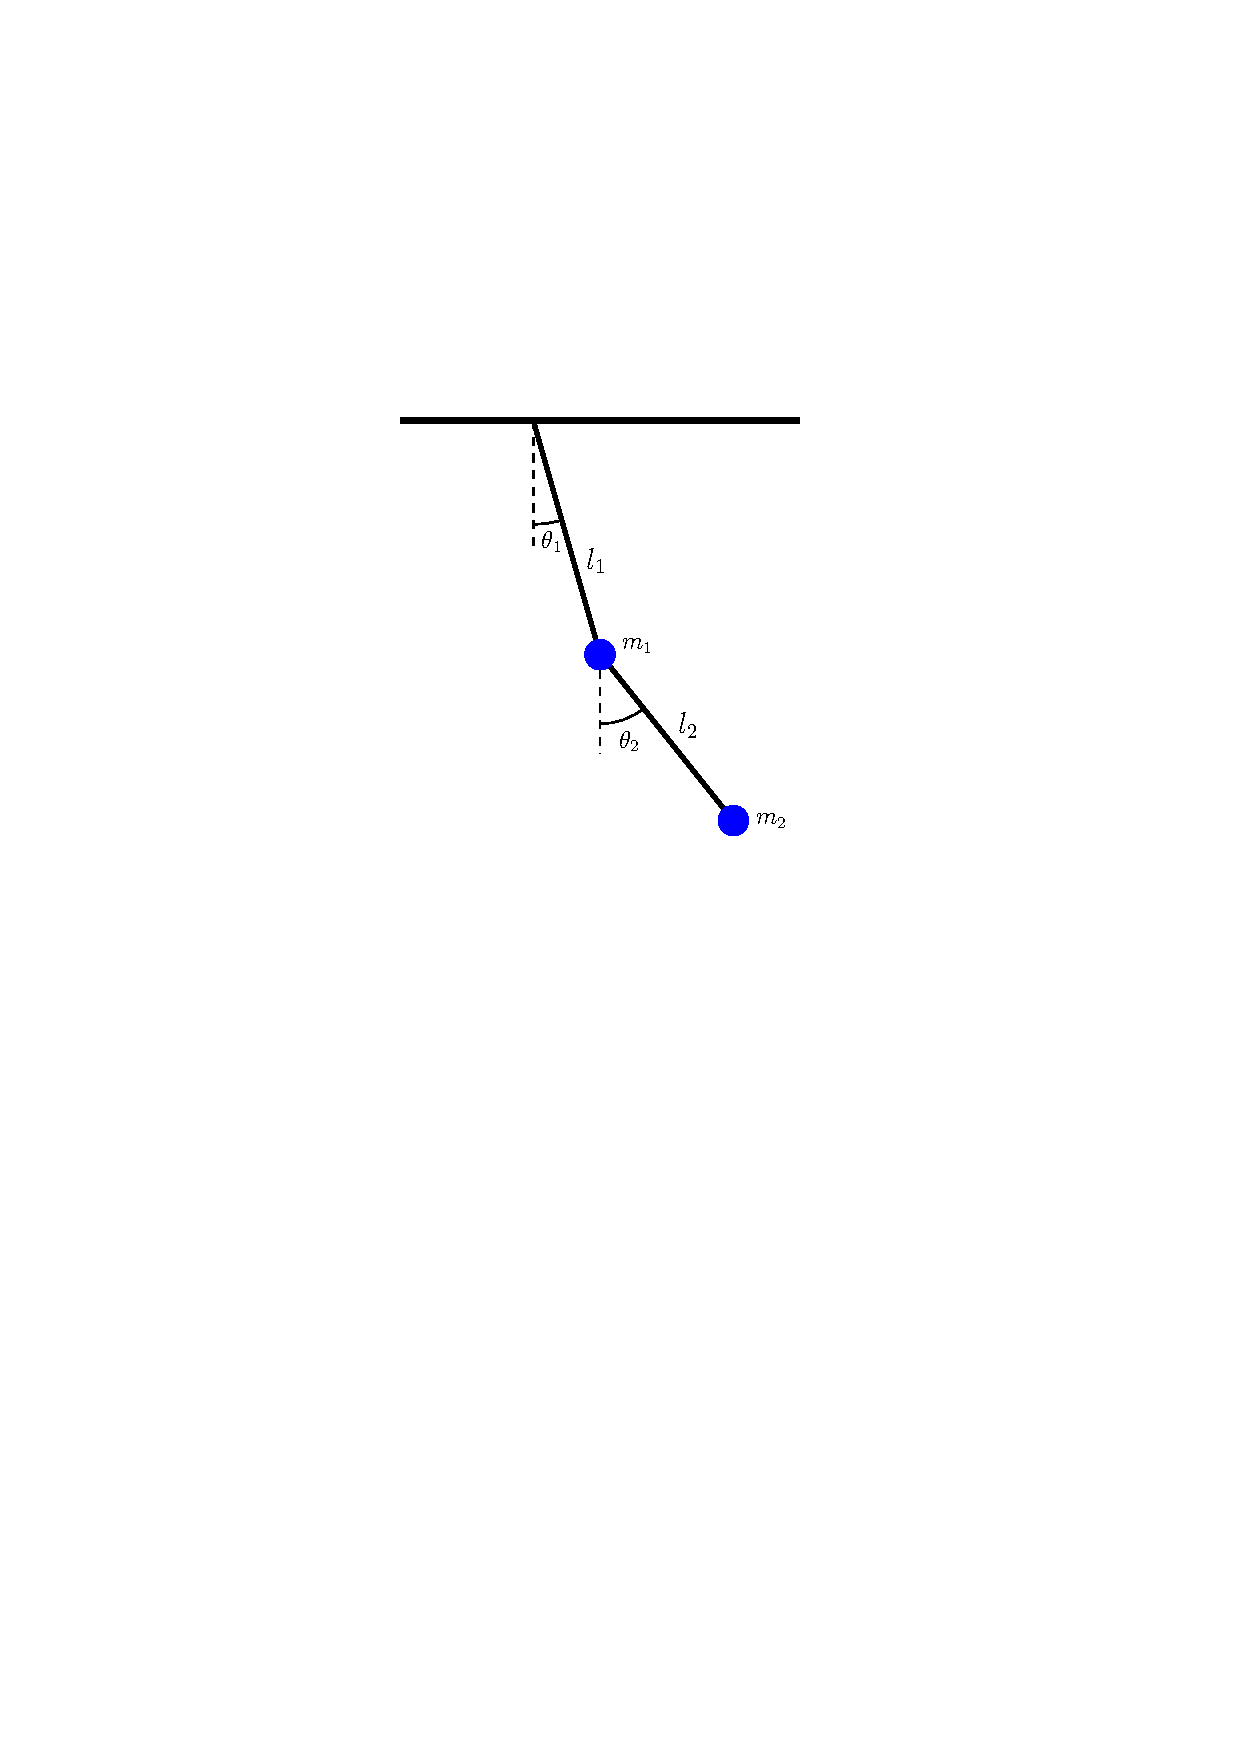
\includegraphics[width=0.45\textwidth]{pic/double pendulum.pdf}
        \caption{Double Pendulum}
        \label{double pendulum}
    \end{figure}
    为方便阅读, 本例中使用黑体字母表示向量.

    {\bf 牛顿力学:} 以双摆的悬挂点为原点, 用 $ \mathbf{r} $ 来表示小球的坐标, 则 
    \begin{align*}
        \mathbf{r}_1 &= l_1(\sin\theta_1,\cos\theta_1),\\
        \dot{\mathbf{r}}_1 &= l_1\dot{\theta}_1(\cos\theta_1,-\sin\theta_1),\\ 
        \ddot{\mathbf{r}}_1 &= l_1\ddot{\theta}_1(\cos\theta_1,-\sin\theta_1)-l_1\dot{\theta}_1^2(\sin\theta_1,\cos\theta_1),\\[2ex]
        \mathbf{r}_2 &= \mathbf{r}_1+l_2(\sin\theta_2,\cos\theta_2),\\
        \dot{\mathbf{r}}_2 &= \dot{\mathbf{r}}_1+l_2\dot{\theta}_2(\cos\theta_2,-\sin\theta_2),\\ 
        \ddot{\mathbf{r}}_2 &= \ddot{\mathbf{r}}_1+l_2\ddot{\theta}_2(\cos\theta_2,-\sin\theta_2)-l_2\dot{\theta}_2^2(\sin\theta_2,\cos\theta_2).
    \end{align*}

    设两个杆上的张力大小分别为 $ T_1 $ 和 $ T_2 $, 则两小球所受的力分别为
    \begin{align*}
        \mathbf{F}_1 &= T_1\frac{-\mathbf{r}_1}{|\mathbf{r}_1|}+T_2\frac{\mathbf{r}_2-\mathbf{r}_1}{|\mathbf{r}_2-\mathbf{r}_1|}+m_1\mathbf{g}=-\frac{T_1}{l_1}\mathbf{r}_1+\frac{T_2}{l_2}(\mathbf{r}_2-\mathbf{r}_1)+m_1\mathbf{g},\\ 
        \mathbf{F}_2 &= T_2\frac{-(\mathbf{r}_2-\mathbf{r}_1)}{|\mathbf{r}_2-\mathbf{r}_1|}+m_2\mathbf{g}=-\frac{T_2}{l_2}(\mathbf{r}_2-\mathbf{r}_1)+m_2\mathbf{g},
    \end{align*}
    带入牛顿定律 $ \mathbf{F}=m\ddot{\mathbf{r}} $ 得到两个方程
    \begin{align*}
        m_1\ddot{\mathbf{r}} &= -\frac{T_1}{l_1}\mathbf{r}_1+\frac{T_2}{l_2}(\mathbf{r}_2-\mathbf{r}_1)+m_1\mathbf{g},\\ 
        m_2\ddot{\mathbf{r}} &= -\frac{T_2}{l_2}(\mathbf{r}_2-\mathbf{r}_1)+m_2\mathbf{g},
    \end{align*}
    按照坐标分量写出来是四个微分方程
    \begin{align*}
        m_1l_1\left( \ddot{\theta}_1\cos\theta_1-\dot{\theta}_1^2\sin\theta_1 \right) &= -T_1\sin\theta_1+T_2\sin\theta_2,\\ 
        -m_1l_1\left( \ddot{\theta}_1\sin\theta_1+\dot{\theta}_1^2\cos\theta_1 \right) &=-T_1\cos\theta_1+T_2\cos\theta_2+m_1g,
    \end{align*}
    \vspace{-1.2cm}
    \begin{align*}
        m_2\left( l_1\ddot{\theta}_1\cos\theta_1-l_1\dot{\theta}_1^2\sin\theta_1+l_2\ddot{\theta}_2\cos\theta_1-l_2\dot{\theta}_2^2\sin\theta_2 \right) &= -T_2\sin\theta_2,\\ 
        -m_2\left( l_1\ddot{\theta}_1\sin\theta_1+l_1\dot{\theta}_1^2\cos\theta_1+l_2\ddot{\theta}_2\sin\theta_1+l_2\dot{\theta}_2^2\cos\theta_2 \right) &= -T_2\cos\theta_2+m_2g,
    \end{align*}
    其中有四个变量 $ \theta_1,\theta_2,T_1,T_2 $.

    分别对前两个和后两个方程以三角函数为系数做线性组合, 可将方程组转化为
    \begin{align*}
        l_1\ddot{\theta}_1 &= \frac{T_2}{m_1}\sin(\theta_2-\theta_1)-g\sin\theta_1,\\
        l_1\dot{\theta}_1^2 &= \frac{T_1}{m_1}-\frac{T_2}{m_1}\cos(\theta_2-\theta_1)-g\cos\theta_1,
    \end{align*}
    \vspace{-1.1cm}
    \begin{align*}
        l_1\ddot{\theta}_1\cos(\theta_2-\theta_1)+l_1\dot{\theta}_1^2\sin(\theta_2-\theta_1)+l_2\ddot{\theta}_2 &= -g\sin\theta_2,\\ 
        -l_1\ddot{\theta}_1\sin(\theta_2-\theta_1)+l_1\dot{\theta}_1^2\cos(\theta_2-\theta_1)+l_2\dot{\theta}_2 &= \frac{T_2}{m_2}-g\cos\theta_2.
    \end{align*}
    关注方程左侧, 在后两个方程中减去前两个方程的成分得
    \begin{align*}
        l_2\ddot{\theta}_2 &= -g\sin\theta_2-\left[ \frac{T_2}{m_1}\sin(\theta_2-\theta_1)-g\sin\theta_1 \right]\cos(\theta_2-\theta_1)\\ 
        &\phantom{=}\;-\left[ \frac{T_1}{m_1}-\frac{T_2}{m_1}\cos(\theta_2-\theta_1)-g\cos\theta_1 \right]\sin(\theta_2-\theta_1)\\ 
        &=-\frac{T_1}{m_1}\sin(\theta_2-\theta_1),
    \end{align*}
    \begin{align*}
        l_2\dot{\theta}_2 &= \frac{T_2}{m_2}-g\cos\theta_2 +\left[ \frac{T_2}{m_1}\sin(\theta_2-\theta_1)-g\sin\theta_1 \right]\sin(\theta_2-\theta_1)\\ 
        &\phantom{=}\;-\left[ \frac{T_1}{m_1}-\frac{T_2}{m_1}\cos(\theta_2-\theta_1)-g\cos\theta_1 \right]\cos(\theta_2-\theta_1)\\ 
        &=\frac{T_2}{m_2}+\frac{T_2}{m_1}-\frac{T_1}{m_1}\cos(\theta_2-\theta_1).
    \end{align*}
    现可将方程组改写为
    \begin{align*}
        l_1\ddot{\theta}_1 &= \frac{T_2}{m_1}\sin(\theta_2-\theta_1)-g\sin\theta_1,\\
        l_1\dot{\theta}_1^2 &= \frac{T_1}{m_1}-\frac{T_2}{m_1}\cos(\theta_2-\theta_1)-g\cos\theta_1,\\ 
        l_2\ddot{\theta}_2 &= -\frac{T_1}{m_1}\sin(\theta_2-\theta_1),\\ 
        l_2\dot{\theta}_2^2 &= \frac{T_2}{m_2}+\frac{T_2}{m_1}-\frac{T_1}{m_1}\cos(\theta_2-\theta_1).
    \end{align*}
    根据第一个和第三个方程, 可以用 $ \theta_1,\theta_2 $ 来表示 $ T_1,T_2 $:
    \begin{align*}
        T_1 &= -m_1\frac{l_2\ddot{\theta}_2}{\sin(\theta_2-\theta_1)},\\ 
        T_2 &= m_1\frac{l_1\ddot{\theta}_1+g\sin\theta_1}{\sin(\theta_2-\theta_1)},
    \end{align*}
    将其带入另外两个方程就得到了双摆的运动方程
    \begin{align*}
        -l_1\dot{\theta}_1^2\sin(\theta_2-\theta_1) &= l_2\ddot{\theta}_2+l_1\ddot{\theta}_1\cos(\theta_2-\theta_1)+g\sin\theta_2\\ 
        l_2\dot{\theta}_2^2\sin(\theta_2-\theta_1) &= \left( \frac{m_1}{m_2}+1 \right)\left( l_1\ddot{\theta}_1+g\sin\theta_1 \right)+l_2\ddot{\theta}_2\cos(\theta_2-\theta_1).
    \end{align*}

    {\bf 拉格朗日力学:} 首先在广义坐标 $ \theta_1,\theta_2 $ 下写出动能和势能
    \begin{align*}
        T &= \frac{1}{2}m_1\dot{\mathbf{r}}_1^2+\frac{1}{2}m_2\dot{\mathbf{r}}_2^2\\ 
        &= \frac{1}{2}m_1l_1^2\dot{\theta}_1^2+\frac{1}{2}m_2\left[ l_1^2\dot{\theta}_1^2+l_2^2\dot{\theta}_2^2+2l_1l_2\dot{\theta}_1\dot{\theta}_2\cos(\theta_2-\theta_1) \right]\\ 
        &= \frac{1}{2}(m_1+m_2)l_1^2\dot{\theta}_1^2+\frac{1}{2}m_2l_2^2\dot{\theta}_2^2+m_2l_1l_2\dot{\theta}_1\dot{\theta}_2\cos(\theta_2-\theta_1),\\
        V &= -m_1gy_1-m_2gy_2 \\ 
        &= -m_1gl_1\cos\theta_1-m_2g(l_1\cos\theta_1+l_2\cos\theta_2)\\ 
        &= -(m_1+m_2)gl_1\cos\theta_1-m_2gl_2\cos\theta_2,
    \end{align*}
    其中 $ y_1,y_2 $ 表示两小球到悬挂点的纵向距离, 于是拉格朗日量为
    \begin{align*}
        L &= T-V\\ 
        &= \frac{1}{2}(m_1+m_2)l_1^2\dot{\theta}_1^2+\frac{1}{2}m_2l_2^2\dot{\theta}_2^2+m_2l_1l_2\dot{\theta}_1\dot{\theta}_2\cos(\theta_2-\theta_1)\\ 
        &\phantom{=}\;+(m_1+m_2)gl_1\cos\theta_1+m_2gl_2\cos\theta_2.
    \end{align*}

    计算关于 $ \theta_1 $ 的拉格朗日方程中的项:
    \begin{align*}
        \frac{\partial L}{\partial\dot{\theta}_1} &= (m_1+m_2)l_1^2\dot{\theta}_1+m_2l_1l_2\dot{\theta}_2\cos(\theta_2-\theta_1),\\ 
        \frac{\mathrm{d}}{\mathrm{d}t}\frac{\partial L}{\partial\dot{\theta}_1} &= (m_1+m_2)l_1^2\ddot{\theta}_1+m_2l_1l_2\ddot{\theta}_2\cos(\theta_2-\theta_1)\\ 
        &\phantom{=}\;-m_2l_1l_2\dot{\theta}_2^2\sin(\theta_2-\theta_1)+m_2l_1l_2\dot{\theta}_1\dot{\theta}_2\sin(\theta_2-\theta_1),\\ 
        \frac{\partial L}{\partial\theta_1} &= m_2l_1l_2\dot{\theta}_1\dot{\theta}_2\sin(\theta_2-\theta_1)-(m_1+m_2)gl_1\sin\theta_1,
    \end{align*}
    写出关于 $ \theta_1 $ 的拉格朗日方程:
    \begin{align*}
        0 &= \frac{\mathrm{d}}{\mathrm{d}t}\frac{\partial L}{\partial\dot{\theta}_1}-\frac{\partial L}{\partial\theta_1}\\ 
        &= (m_1+m_2)l_1^2\ddot{\theta}_1+m_2l_1l_2\ddot{\theta}_2\cos(\theta_2-\theta_1)\\ 
        &\phantom{=}\;-m_2l_1l_2\dot{\theta}_2^2\sin(\theta_2-\theta_1)+(m_1+m_2)gl_1\sin\theta_1.
    \end{align*}
    计算关于 $ \theta_2 $ 的拉格朗日方程中的项:
    \begin{align*}
        \frac{\partial L}{\partial\dot{\theta_2}} &= m_2l_2^2\dot{\theta}_2+m_2l_1l_2\dot{\theta}_1\cos(\theta_2-\theta_1),\\ 
        \frac{\mathrm{d}}{\mathrm{d}t}\frac{\partial L}{\partial\dot{\theta}_2} &= m_2l_2^2\ddot{\theta}_2+m_2l_1l_2\ddot{\theta}_1\cos(\theta_2-\theta_1)\\ 
        &\phantom{=}\;+m_2l_1l_2\dot{\theta}_1^2\sin(\theta_2-\theta_1)-m_2l_1l_2\dot{\theta}_1\dot{\theta}_2\sin(\theta_2-\theta_1),\\ 
        \frac{\partial L}{\partial\theta_2} &= -m_2l_1l_2\dot{\theta}_1\dot{\theta}_2\sin(\theta_2-\theta_1)-m_2gl_2\sin\theta_2,
    \end{align*}
    写出关于 $ \theta_2 $ 的拉格朗日方程:
    \begin{align*}
        0 &= \frac{\mathrm{d}}{\mathrm{d}t}\frac{\partial L}{\partial\dot{\theta_2}}-\frac{\partial L}{\partial\theta_2}\\ 
        &= m_2l_2^2\ddot{\theta}_2+m_2l_1l_2\ddot{\theta}_1\cos(\theta_2-\theta_1)+m_2l_1l_2\dot{\theta}_1^2\sin(\theta_2-\theta_1)+m_2gl_2\sin\theta_2.
    \end{align*}

    这两个拉格朗日方程正是我们前面用牛顿定律推出的运动方程!
\end{example}
虽然两种方法得到了同样的结果, 但使用牛顿力学处理该问题时, 需要用到各种数学技巧, 处理起来也比较麻烦. 在使用拉格朗日力学时, 只需要按部就班地计算就能得到所需的答案.
\section{流形上的拉格朗日力学}
我们可以将拉格朗日力学推广到流形上, 即设位形空间 $ M $ 为光滑流形, 拉格朗日量为其切丛上的光滑函数 $ L(q,\dot{q}):TM\to\mathbb{R} $, 此时仍可推出拉格朗日方程, 但要注意 $ \frac{\partial L}{\partial q} $ 和 $ \frac{\partial L}{\partial\dot{q}} $ 是余切向量.

\begin{remark}
    对于黎曼流形, 可将动能定义为切丛上的二次型 $ \frac{m}{2}\langle \dot{q},\dot{q} \rangle $.
\end{remark}

本节的目的是介绍一个非常重要的定理, 即诺特定理, 它指出每个拉格朗日函数的对称性都有对应的守恒律, 其中守恒律指的是某个物理量不随时间变化.

令 $ h:M\to M $ 为一光滑映射, 若 $ L(h(x),h_{*x}(v))=L(x,v) $, $ \forall(x,v)\in TM$, 其中 $ h_{*x} $ 是 $ h $ 在点 $ x $ 处的切映射 (推出), 则称拉格朗日系统 $ (M,L) $ 容许映射 $ h $.

\begin{theorem}[诺特定理]
    若系统 $ (M,L) $ 容许一个单参微分同胚群 $ h^s:M\to M $, $ s\in\mathbb{R} $, 则切丛上的函数
    \[ I(q,\dot{q}):=\left.\frac{\partial L}{\partial\dot{q}}\frac{\mathrm{d}h^s(q)}{\mathrm{d}s}\right|_{s=0} \]
    是守恒量, 即满足
    \[ \frac{\mathrm{d}}{\mathrm{d}t}I(q,\dot{q})=0. \]
\end{theorem}

\begin{remark}
    $ \dfrac{\partial L}{\partial\dot{q}} $ 是余切向量, $ \left.\dfrac{\mathrm{d}h^s(q)}{\mathrm{d}s}\right|_{s=0} $ 是切向量.
\end{remark}

\begin{proof}
    若 $ h $ 是微分同胚且 $ L(h(x),h_{*x}(v))=L(x,v) $, $ \forall(x,v)\in TM$, 则两边同时求梯度有
    \begin{align*}
        \frac{\partial L(x,v)}{\partial x} &= h^*_x\frac{\partial L(h(x),h_{*x}(v))}{\partial q},\\
        \frac{\partial L(x,v)}{\partial v} &= h^*_x\frac{\partial L(h(x),h_{*x}(v))}{\partial\dot{q}}.
    \end{align*}
    设 $ \varphi(t) $ 是拉格朗日方程的解, 即满足
    \[ \frac{\partial L(\varphi,\dot{\varphi})}{\partial q}=\frac{\mathrm{d}}{\mathrm{d}t}\frac{\partial L(\varphi,\dot{\varphi})}{\partial\dot{q}}. \]
    由于 $ h $ 是微分同胚, 其诱导的拉回映射 $ h^* $ 是可逆的, 进而有
    \[ \frac{\partial L(h(\varphi),h_{*\varphi}(\dot{\varphi}))}{\partial q}=\frac{\mathrm{d}}{\mathrm{d}t}\frac{\partial L(h(\varphi),h_{*\varphi}(\dot{\varphi}))}{\partial\dot{q}}, \]
    这说明 $ h $ 将拉格朗日方程的解映为解. (这也说明拉格朗日方程不依赖于坐标选取.)

    记 $ \Phi(s,t)=h^s(\varphi(t)) $, 由前面的讨论有
    \[ \frac{\partial L(\Phi,\dot{\Phi})}{\partial q}=\frac{\mathrm{d}}{\mathrm{d}t}\frac{\partial L(\Phi,\dot{\Phi})}{\partial\dot{q}}. \]
    用 $ ' $ 表示对 $ s $ 求导, 由于 $ h^s $ 保持 $ L $,
    \begin{align*}
        0 &= \frac{\partial L(\Phi,\dot{\Phi})}{\partial s}=\frac{\partial L(\Phi,\dot{\Phi})}{\partial q}\Phi'+\frac{\partial L(\Phi,\dot{\Phi})}{\partial\dot{q}}\dot{\Phi}'\\ 
        &= \left( \frac{\mathrm{d}}{\mathrm{d}t}\frac{\partial L(\Phi,\dot{\Phi})}{\partial\dot{q}} \right)\Phi'+\frac{\partial L(\Phi,\dot{\Phi})}{\partial\dot{q}}\left( \frac{\mathrm{d}}{\mathrm{d}t}\Phi' \right)\\ 
        &= \frac{\mathrm{d}}{\mathrm{d}t}\left( \frac{\partial L(\Phi,\dot{\Phi})}{\partial\dot{q}}\Phi' \right),
    \end{align*}
    其中由于单参微分同胚群是光滑的, $ \Phi $ 对 $ s $ 和对 $ t $ 求导可换序. 当固定 $ s=0 $ 时有
    \[ \frac{\partial L(\varphi,\dot{\varphi})}{\partial\dot{q}}\left.\frac{\mathrm{d}h^s(q)}{\mathrm{d}s}\right|_{s=0}, \]
    这正是我们想找的 $ I $. 
\end{proof}
接下来, 我们计算两个关于 $ \mathbb{R}^3 $ 上拉格朗日函数 $ L(q,\dot{q})=\frac{1}{2}m\dot{q}^2-V(q) $ 的例子.
\begin{example}[动量守恒]
    若 $ L $ 容许沿空间向量 $ r $ 平移, 即 $ h^s(q)=q+sr $, 则
    \[ I(q,\dot{q})=m\dot{q}\cdot r, \]
    这是{\bf 动量} $ p=m\dot{q} $ 在方向 $ r $ 上的分量.
\end{example}
\begin{example}[角动量守恒]
    若 $ L $ 容许绕单位向量 $ \omega $ 所在直线旋转, 使用 Rodrigues' rotation formula:
    \begin{align*}
        h^\theta(q) &= q_{\perp}\cos\theta+(\omega\times q)\sin\theta+q_{\parallel}\\ 
        &=[q-(\omega\cdot q)\omega]\cos\theta+(\omega\times q)\sin\theta+(\omega\cdot q)\omega.
    \end{align*}
    则
    \[ I(q,\dot{q})=p\cdot(\omega\times q)=\omega\cdot(q\times p), \]
    这是{\bf 角动量} $ q\times p $ 在 $ \omega $ 上的分量. 若该系统正是绕 $ \omega $ 所在直线旋转的, 则 $ q\times p $ 与 $ \omega $ 共线, 进而有角动量 $ q\times p $ 守恒.
\end{example}
\begin{remark}
    由于
    \[ u\times v=\left( \begin{matrix}
        u_yv_z-u_zv_y \\ u_zv_x-u_xv_z \\ u_xv_y-u_yv_x
    \end{matrix} \right)=\left( \begin{matrix}
        0 & -u_z & u_y \\ 
        u_z & 0 & -u_x \\ 
        -u_y & u_x & 0
    \end{matrix} \right)v \]
    和
    \[ (u\cdot v)u=\left( \begin{matrix}
        u_x^2 & u_xu_y & u_xu_z \\ 
        u_xu_y & u_y^2 & u_yu_z \\ 
        u_xu_z & u_yu_z & u_z^2
    \end{matrix} \right)v, \]
    还可将 $ h^\theta(q) $ 写成矩阵形式 $ h^\theta(q)=Rq $.
\end{remark}
\section{哈密顿力学}

对于凸函数 $ f $, 其{\bf 共轭函数}为
\[ f^*(y):=\sup_{x\in C}(\langle y,x \rangle-f(x)),\quad y\in \mathrm{dom}f^*, \]
其中 
\[ \mathrm{dom}f^*=\left\{ y\in\mathbb{R}^n \;\middle|\; \sup_{x\in C}(\langle y,x \rangle-f(x))<\infty \right\}. \]
共轭函数 $ f^* $ 也是凸函数, 且若 $ f $ 是闭的, 则 $ f^{**}=f $. 

当 $ f $ 可微时, 共轭函数 $ f^* $ 也叫做 $ f $ 的勒让德变换, 若 $ f $ 还是严格凸的则 $ f^* $ 可表达为
\[ f^*(p)=\left[\langle p,x \rangle-f(x)\right]\big|_{x=(\nabla f)^{-1}(p)}.\]

考虑位形空间为 $ \mathbb{R}^n $ 时的经典力学.

\begin{definition}[哈密顿量]
{\bf 哈密顿量}是对拉格朗日函数 $ L(q,\dot{q})=\frac{1}{2}m\dot{q}^2-V(q) $ 做关于变量 $ \dot{q} $ 的勒让德变换所得的函数, 即
\begin{align*}
    H(q,p) :&= \frac{p^2}{2m}+V(q)=T+V\\ 
    &= p\cdot\dot{q}-L(q,\dot{q}).
\end{align*}
\end{definition}

我们称 $ q $ 和 $ p $ 共同构成的 $ 2n $ 维空间为相空间, 哈密顿量是相空间上的函数. 由于哈密顿量等于动能加势能, 它的物理含义就是{\bf 能量}. 

\begin{theorem}
    拉格朗日方程等价于下述方程组
    \begin{align*}
        \dot{q}&=\frac{\partial H}{\partial p},\\
        \dot{p}&=-\frac{\partial H}{\partial q},
    \end{align*}
    这个方程组叫做{\bf 哈密顿方程}.
\end{theorem}
\begin{remark}
    拉格朗日方程是 $ n $ 个二阶方程, 而哈密顿方程是 $ 2n $ 个一阶方程.
\end{remark}
\begin{proof}
$ H(q,p) $ 的全微分
\[ \mathrm{d}H=\frac{\partial H}{\partial p}\mathrm{d}p+\frac{\partial H}{\partial q}\mathrm{d}q, \]
应等于 $ p\cdot\dot{q}-L $ 的全微分
\[ \dot{q}\mathrm{d}p-\frac{\partial L}{\partial q}\mathrm{d}q, \]
若 $ q(t) $ 满足拉格朗日方程, 则
\[ \dot{q}=\frac{\partial H}{\partial p},\quad \dot{p}=-\frac{\partial H}{\partial q}. \]

反之, $ L(q,\dot{q}) $ 的全微分
\[ \mathrm{d}L=\frac{\partial L}{\partial q}\mathrm{d}q+\frac{\partial L}{\partial\dot{q}}\mathrm{d}\dot{q} \]
应等于 $ p\cdot\dot{q}-H $ 的全微分
\[ -\frac{\partial H}{\partial q}\mathrm{d}q+p\mathrm{d}\dot{q}, \]
若 $ (q(t),p(t)) $ 满足哈密顿方程, 则 $ q(t) $ 满足拉格朗日方程.
\end{proof}
\begin{corollary}[能量守恒]\keepline
    \[ \frac{\mathrm{d}H}{\mathrm{d}t}=0. \] 
\end{corollary}
\vspace{0ex}
\begin{proof}\keepline
    \begin{align*}
        \frac{\mathrm{d}H}{\mathrm{d}t} &= \frac{\partial H}{\partial q}\cdot{\dot{q}}+\frac{\partial H}{\partial p}\cdot{\dot{p}}\\ 
        &= \frac{\partial H}{\partial q}\cdot\frac{\partial H}{\partial p}-\frac{\partial H}{\partial p}\cdot\frac{\partial H}{\partial q}\\ 
        &= 0.\qedhere
    \end{align*}
\end{proof}

对于 $ \mathbb{R}^n $ 上的常微分方程组 $ \dot{x}=f(x) $, 称单参变换群 $ \varphi_t:x(0)\mapsto x(t) $ 为相流. 对任意区域 $ D $, 记
\[ D(t):=\varphi_t(D),\quad v(t):=\int_{D(t)}\mathrm{d}V, \]
则 $v(t)$ 表示了区域 $D$ 随体积随时间变化的情况.

特别地, 哈密顿方程诱导了相空间中的相流. 若将相空间直观地想象为流体, 则哈密顿方程描述了其流动方式. 一个十分神奇的事情是: 相空间是不可压缩流体! 这个结论叫做刘维尔定理, 在统计力学中有重要应用. 为了严格证明它, 我们要先证明一个更一般的结论.

\begin{theorem}
    若 $ \nabla\cdot f=0 $ ($f$ 的散度为 $0$), 则 $\dot{x}=f(x)$ 对应的相流保持体积, 即任意区域的体积 $v(t)$ 为常值函数.
\end{theorem}

\begin{proof}
    首先通过坐标变换有
    \[ v(t)=\int_{D(0)}\mathrm{det}\left( \frac{\partial\varphi_t(x)}{\partial x} \right)\mathrm{d}V. \]
    将 $ \varphi_t $ 展开为
    \[ \varphi_t(x)=x(t)=x+f(x)t+O(t^2), \]
    两边同时对 $ x $ 求导得
    \[ \frac{\partial\varphi_t(x)}{\partial x} = I+\frac{\partial f(x)}{\partial x}t+O(t^2), \]
    应用
    \[ \mathrm{det}(I+tA)=1+t\mathrm{Tr}(A)+O(t^2) \]
    可得
    \[ \mathrm{det}\left( \frac{\partial\varphi_t(x)}{\partial x} \right)=1+t\mathrm{Tr}\left( \frac{\partial f(x)}{\partial x} \right)+O(t^2). \]
    由于
    \[ \mathrm{Tr}\left( \frac{\partial f(x)}{\partial x} \right)=\nabla\cdot f, \]
    我们有
    \[ v(t)=\int_{D(0)}\left[ 1+t\nabla\cdot f+O(t^2) \right]\,\mathrm{d}V, \]
    因此
    \[ \left.\frac{\mathrm{d}v(t)}{\mathrm{d}t}\right|_{t=0}=\int_{D(0)}\nabla\cdot f\,\mathrm{d}V. \]
    上述证明中的 $ t=0 $ 可替换为任意 $ t=t_0 $, 因此 
    \[ \frac{\mathrm{d}v}{\mathrm{d}t}=0,\quad v(t)=v(0),\quad\forall t\in\mathbb{R}.\qedhere \]
\end{proof}

\begin{corollary}[刘维尔定理]
    哈密顿相流保持体积不变
\end{corollary}
\begin{proof}\keepline
    \[ \sum_{i=1}^{n}\frac{\partial^2 H}{\partial q_i\partial p_i}-\sum_{i=1}^{n}\frac{\partial^2 H}{\partial p_i\partial q_i}=0.\qedhere \]
\end{proof}

\begin{definition}[泊松括号]
    在坐标 $ (q,p) $ 下, 相空间上的光滑函数 $f,g$ 的{\bf 泊松括号} (Poisson bracket) 为
    \[ \{f,g\}:=\sum_{i=1}^{n}\left( \frac{\partial f}{\partial q_i}\frac{\partial g}{\partial p_i}-\frac{\partial f}{\partial p_i}\frac{\partial g}{\partial q_i} \right). \]
\end{definition}

\begin{proposition}
    泊松括号满足
    \begin{enumerate}
        \item $ \{f,g+ch\}=\{f,g\}+c\{f,h\} $, $ \forall c\in\mathbb{R} $;
        \item $ \{f,g\}=-\{g,f\} $;
        \item $ \{f,\{g,h\}\}+\{h,\{f,g\}\}+\{g,\{h,f\}\}=0 $;
        \item $ \{f,gh\}=\{f,g\}h+\{f,h\}g $.
    \end{enumerate}
\end{proposition}

前两条说明泊松括号是双线性的, 第三条叫做{\bf 雅克比恒等式} (Jacobi identity), 前三条性质说明相空间上的光滑函数配上泊松括号构成一个李代数, 李代数的定义可见附录 \ref{lie}.

\begin{proposition}\keepline
    \[ \dot{f}=\frac{\mathrm{d}}{\mathrm{d}t}f=\{f,H\}. \]
\end{proposition}
\vspace{0ex}
\begin{corollary}
    相空间上的光滑函数 $ f $ 为守恒量当且仅当 $ \{f,H\}=0$.
\end{corollary}
\vspace{0ex}
\begin{proposition}\keepline
    \label{commutation}
    \[\begin{aligned}
        \{q_i,q_j\} &= 0,\\ 
        \{p_i,p_j\} &= 0,\\ 
        \{q_i,p_j\} &= \delta_{ij}.
    \end{aligned}\]
\end{proposition}
\vspace{0ex}
拉格朗日方程不依赖于位形空间的坐标选取, 但哈密顿方程没有这么好的性质. 这是因为相空间上有特殊的结构 (辛结构), 一般的坐标变换会破坏它.

\begin{definition}
    对于坐标变换 $ (q,p)\mapsto(Q,P) $, 若 $ Q(q,p) $ 和 $ P(q,p) $ 满足命题 \ref{commutation} 中的对易关系, 即
    \[ \{Q_i,Q_j\}=0,\quad\{P_i,P_j\}=0,\quad\{Q_i,P_i\}=\delta_{ij}, \]
    则称该坐标变换为{\bf 正则变换}, 称通过正则变换得到的坐标为{\bf 正则坐标}.
\end{definition}

\begin{theorem}
    正则变换保持泊松括号不变, 即对于坐标 $ (q,p) $ 和 $ (Q,P) $ 下定义的泊松括号 $ \{f,g\}_{(q,p)} $ 和 $ \{f,g\}_{(Q,P)} $, 有
    \[ \{f,g\}_{(q,p)}=\{f,g\}_{(Q,P)}. \]
\end{theorem}
\begin{proof}
    将
    \begin{align*}
        \frac{\partial f}{\partial q_i} &= \sum_{j=1}^{n}\left( \frac{\partial f}{\partial Q_j}\frac{\partial Q_j}{\partial q_i}+\frac{\partial f}{\partial P_j}\frac{\partial P_j}{\partial q_i} \right), &
        \frac{\partial f}{\partial p_i} &= \sum_{j=1}^{n}\left( \frac{\partial f}{\partial Q_j}\frac{\partial Q_j}{\partial p_i}+\frac{\partial f}{\partial P_j}\frac{\partial P_j}{\partial p_i} \right), \\
        \frac{\partial g}{\partial q_i} &= \sum_{k=1}^{n}\left( \frac{\partial g}{\partial Q_k}\frac{\partial Q_k}{\partial q_i}+\frac{\partial g}{\partial P_k}\frac{\partial P_k}{\partial q_i} \right), &
        \frac{\partial g}{\partial p_i} &= \sum_{k=1}^{n}\left( \frac{\partial g}{\partial Q_k}\frac{\partial Q_k}{\partial p_i}+\frac{\partial g}{\partial P_k}\frac{\partial P_k}{\partial p_i} \right),
    \end{align*}
    带入 $ \{f,g\}_{(q,p)} $ 有
    \begin{align*}
        &\phantom{=}\;\;\{f,g\}_{(q,p)}\\[2pt]
        &= \sum_{i=1}^{n}\left( \frac{\partial f}{\partial q_i}\frac{\partial g}{\partial p_i}-\frac{\partial f}{\partial p_i}\frac{\partial g}{\partial q_i} \right)\\
        &= \sum_{i,j,k=1}^{n}\left[ \left( \frac{\partial f}{\partial Q_j}\frac{\partial Q_j}{\partial q_i}+\frac{\partial f}{\partial P_j}\frac{\partial P_j}{\partial q_i} \right)\left( \frac{\partial g}{\partial Q_k}\frac{\partial Q_k}{\partial p_i}+\frac{\partial g}{\partial P_k}\frac{\partial P_k}{\partial p_i} \right)\right.\\ 
        &\hspace{32.7pt}-\left.\left( \frac{\partial f}{\partial Q_j}\frac{\partial Q_j}{\partial p_i}+\frac{\partial f}{\partial P_j}\frac{\partial P_j}{\partial p_i} \right)\left( \frac{\partial g}{\partial Q_k}\frac{\partial Q_k}{\partial q_i}+\frac{\partial g}{\partial P_k}\frac{\partial P_k}{\partial q_i} \right)\right]\\[2pt]
        &=\sum_{i,j,k=1}^{n}\left[\frac{\partial f}{\partial Q_j}\frac{\partial g}{\partial Q_k}\left( \frac{\partial Q_j}{\partial q_i}\frac{\partial Q_k}{\partial p_i}-\frac{\partial Q_j}{\partial p_i}\frac{\partial Q_k}{\partial q_i} \right) + \frac{\partial f}{\partial P_j}\frac{\partial g}{\partial P_k}\left( \frac{\partial P_j}{\partial q_i}\frac{\partial P_k}{\partial p_i}-\frac{\partial P_j}{\partial p_i}\frac{\partial P_k}{\partial q_i} \right)\right.\\
        &\hspace{33.9pt}+\frac{\partial f}{\partial Q_j}\frac{\partial g}{\partial P_k}\left( \frac{\partial Q_j}{\partial q_i}\frac{\partial P_k}{\partial p_i}-\frac{\partial Q_j}{\partial p_i}\frac{\partial P_k}{\partial q_i} \right)+\left. \frac{\partial f}{\partial P_j}\frac{\partial g}{\partial Q_k}\left( \frac{\partial P_j}{\partial q_i}\frac{\partial Q_k}{\partial p_i}-\frac{\partial P_j}{\partial p_i}\frac{\partial Q_k}{\partial q_i} \right) \right]\\[2pt]
        &=\sum_{j,k=1}^{n}\left( \frac{\partial f}{\partial Q_j}\frac{\partial g}{\partial Q_k}\{Q_j,Q_k\}_{(q,p)}+\frac{\partial f}{\partial P_j}\frac{\partial g}{\partial P_k}\{P_j,P_k\}_{(q,p)} \right.\\ 
        &\hspace{40.8pt}\left.\frac{\partial f}{\partial Q_j}\frac{\partial g}{\partial P_k}\{Q_j,P_k\}_{(q,p)}+\frac{\partial f}{\partial P_j}\frac{\partial g}{\partial Q_k}\{P_j,Q_k\}_{(q,p)}\right).\\
        &= \sum_{j,k=1}^{n}\left( \frac{\partial f}{\partial Q_j}\frac{\partial g}{\partial P_k}\delta_{jk}-\frac{\partial f}{\partial P_j}\frac{\partial g}{\partial Q_k}\delta_{jk} \right)\\ 
        &= \sum_{j=1}^{n}\left( \frac{\partial f}{\partial Q_j}\frac{\partial g}{\partial P_j}-\frac{\partial f}{\partial P_j}\frac{\partial g}{\partial Q_j} \right)\\ 
        &= \{f,g\}_{(Q,P)},
    \end{align*}
    其中第 $5$ 个等号用到了正则变换的定义.
\end{proof}

\begin{theorem}
    正则变换保持哈密顿方程.
\end{theorem}

对于坐标 $ (q,p) $, 定义{\bf 辛标记} (symplectic notation) 为 
\[ \xi:=(q_1,\dots,q_n,p_1,\dots,p_n)^{\mathsf{T}},\] 
或写作
\[ \xi_i=\begin{cases}
    q_i, & i=1,\dots,n\\ 
    p_{i-n}, & i=n+1,\dots,2n
\end{cases}. \]
定义{\bf 辛矩阵}为
\[ \Omega:=\left( \begin{matrix}
    0 & I_n\\ 
    -I_n & 0
\end{matrix} \right), \]
则哈密顿方程可重写为
\[ \dot{\xi}=\Omega\frac{\partial H}{\partial\xi}. \]

记坐标 $ (Q,P) $ 的辛标记为 $ \zeta $, 记坐标变换 $ (q,p)\mapsto(Q,P) $ 的雅克比矩阵为 
\[ M=(M_{ij}):=\left(\dfrac{\partial\zeta_i}{\partial\xi_j}\right).\] 则
\[ \dot{\zeta}=M\dot{\xi},\quad \frac{\partial H}{\partial\xi}=M^{\mathsf{T}}\frac{\partial H}{\partial\zeta}, \]
将它们带入 $ \xi $ 的哈密顿方程有
\[ \dot{\zeta}=M\Omega M^{\mathsf{T}}\frac{\partial H}{\partial\zeta}. \]

因此, 想要让坐标变换保持哈密顿方程, 只需让它满足{\bf 辛条件}, 即
\[ M\Omega M^{\mathsf{T}}=\Omega. \]

\begin{theorem}
    一个坐标变换是正则的当且仅当它满足辛条件.
\end{theorem}
\begin{proof}
    将
    \[ M=\frac{\partial\zeta}{\partial\xi}=\left( \begin{matrix}
        \frac{\partial Q}{\partial q} & \frac{\partial Q}{\partial p}\\ 
        \frac{\partial P}{\partial q} & \frac{\partial P}{\partial p}
    \end{matrix} \right) \]
    带入 $ M\Omega M^{\mathsf{T}} $ 有
    \[M\Omega M^{\mathsf{T}} = \left( \begin{matrix}
            \big(\{Q_i,Q_j\}\big) & \big(\{Q_i,P_j\}\big) \\ 
            \big(\{P_i,Q_j\}\big) & \big(\{P_j,P_j\}\big)
        \end{matrix} \right).\qedhere\]
\end{proof}
\begin{corollary}
    正则变换保持哈密顿方程.
\end{corollary}

综上, 哈密顿力学不依赖于正则坐标的选取.
\section{流形上的哈密顿力学}
待续
\chapter{量子力学}
剧透: 量子力学很大程度上是在研究 $ L^2 $ 空间上的无界自伴算子. 

\setcounter{section}{-1}
\section{预备知识}
我打算先提一些与无界算子相关的概念和结论, 如果读者不是非常在意数学上的严谨性, 可将本节忽略. 

\begin{remark}
    当然, 我们讨论的都是线性算子.
\end{remark}

\begin{theorem}[Hellinger-Toeplitz 定理]
    \label{Hellinger-Toeplitz}
    设 $ A $ 是希尔伯特空间 $ H $ 到自身的处处有定义的线性算子. 若
    \[ \langle Ax,y \rangle=\langle x,Ay \rangle,\quad\forall x,y\in H,\]
    则 $ A $ 是有界的.
\end{theorem}

上述定理指出, 无界算子一定不是处处有定义的. 我们在量子力学中考虑的算子大部分都是无界的, 这让情况变得比较复杂.

\begin{definition}[伴随算子]
    对于无界的稠定 (定义域稠密的) 算子 $ A:H\to H $, 定义其伴随算子 $ A^* $ 如下:
    \begin{enumerate}
        \item 先定义 $ \mathrm{Dom}(A^*) $, 对于 $ \varphi\in H $, 若 $ \mathrm{Dom}(A) $ 上的线性泛函 
        \[ \psi\mapsto \langle \varphi,A\psi\rangle \] 
        是有界的, 则 $ \varphi\in\mathrm{Dom}(A^*) $.
        \item 对于 $ \varphi\in\mathrm{Dom}(A^*) $, 存在唯一的 $ \rchi \in H$ 满足
        \[ \langle \rchi,\psi \rangle=\langle \varphi,A\psi \rangle,\quad\forall\psi\in\mathrm{Dom}(A), \]
        定义 $ A^*\varphi=\rchi $.
    \end{enumerate}
\end{definition}

\begin{definition}
    对于 $ H $ 上的无界稠定算子 $ A $, 定义以下三种性质:
    \begin{enumerate}
        \item 对称 (symmetric): $ \langle \varphi,A\psi \rangle=\langle A\varphi,\psi \rangle $, $ \forall \varphi,\psi,\in\mathrm{Dom}(A) $.
        \item 自伴 (self-adjoint): $ \mathrm{Dom}(A^*)=\mathrm{Dom}(A) $ 且 $ A^*\varphi=A\varphi $, $ \forall\varphi\in\mathrm{Dom}(A) $.
        \item  本质自伴 (essentially self-adjoint): $ A $ 是对称的且 $ A $ 的图像的闭包是某个自伴算子的图像.
    \end{enumerate}
\end{definition}

\begin{proposition}
    无界稠定算子的伴随算子是闭的, 因此自伴算子都是闭的.
\end{proposition}

我们不加证明地指出, 接下来我们遇到的所有算子都是本质自伴的, 因此可通过取闭包来获得自伴的版本, 进而我们可以只考虑自伴算子.

\begin{definition}[谱]
    对于 $ H $ 上的无界算子 $ A $, $ \lambda\in\mathbb{C} $, 我们称 $ \lambda $ 属于 $ A $ 的预解集 (resolvent set), 若存在有界算子 $ B $ 使得
    \begin{enumerate}
        \item $ \forall\psi\in H $, $ B\psi\in\mathrm{Dom}(A) $, $ (A-\lambda I)B\psi=\psi $;
        \item $ \forall\psi\in\mathrm{Dom}(A) $, $ B(A-\lambda I)\psi=\psi $.
    \end{enumerate}
    若不存在这样的 $ B $, 则称 $ \lambda $ 属于 $ A $ 的谱 (spectrum).
\end{definition}

\begin{proposition}
    无界自伴算子的谱是包含于 $ \mathbb{R} $ 的闭集.
\end{proposition}
\section{量子力学公理}
在哈密顿力学中, 系统的状态可由相空间上的点表示, 物理量都是相空间上的函数, 而在量子力学中, 情况则完全不同.
\begin{quantumaxiom}
    系统的状态可用一个可分的复希尔伯特空间 $ H $ 中的向量 $ \psi $ 来表示. 
    
    对于两个向量 $ \psi_1 $, $ \psi_2 $, 若存在 $ c\in\mathbb{C} $ 使得 $ \psi_2=c\psi_1 $, 则它们表示同一个状态. 因此, 不失一般性地, 我们只考虑单位向量.
\end{quantumaxiom}

我们把这个 $ H $ 叫做{\bf 量子希尔伯特空间}. 量子力学主要考虑 $ H=L^2(\mathbb{R}^3) $ 的情况, 唯独在讨论自旋时, 取 $ H=\mathbb{R}^n $.

单位长度的 $ L^2 $ 函数 $ \psi $ 就是物理学家所说的{\bf 波函数} (wave function). 另外, 物理学家会用右矢 (ket) $ |\psi\rangle $ 来表示向量, 用左矢 (bra) $ \langle\psi| $ 来表示对偶向量.

\begin{quantumaxiom}
    {\bf 可观测量}可以用 $ H $ 上的自伴算子来表示, 其中可观测量指的是在现实中可以用物理装置去测量的物理量. 
    
    经典力学中的可观测量是相空间上的实值函数, 对于每个经典可观测量 $ f $, 存在一个对应的 $ H $ 上的自伴算子 $ \hat{f} $, 叫做 $ f $ 对应的量子可观测量.
\end{quantumaxiom}

为 $ f $ 寻找对应的 $ \hat{f} $ 这个行为叫做量子化 (量子化的方案有很多). 

\begin{remark}
    不是所有自伴算子都可观测, 也不是所有量子可观测量都有对应的经典可观测量. 本书考虑的所有物理量都是可观测的.
\end{remark}

物理学家将算子 (operator) 翻译为算符, 将自伴 (self-adjoint) 叫做埃尔米特 (Hermitian), 将酉 (unitary) 翻译为幺正.

\begin{quantumaxiom}
    每次测量可观测量 $ A $ 会得到 $ A $ 的谱中的一个元素, 测量结果服从一个概率分布. 设系统处于状态 $ \psi\in H $, 则该分布的各阶矩满足
    \[ E(A^m)=\langle \psi,A^m\psi \rangle. \]
\end{quantumaxiom}

根据常识, 大部分物理量是可以任意大的, 那么它们对应的算子也应该是无界的, 根据定理 \ref{Hellinger-Toeplitz}, 无界算子的定义域不能是整个 $ H $, 这会让事情变得很复杂. 事实上情况就是这么的残酷! 为了方便讨论, 本书不细究算子的定义域问题. 有关这个问题的严谨讨论见 \cite[第 9 章]{hall2013quantum}.

设可观测量 $ A $ 的谱完全由特征值构成, 其特征值为 $ \lambda_1,\lambda_2,\dots $, 对应的特征向量为 $ e_1,e_2,\dots $, 且这些特征向量构成了 $ H $ 的一组正规正交基. 任给状态 $ \psi $, 做分解
\[ \psi=\sum_{i=1}^{\infty}a_ie_i,\quad a_i=\langle \psi,e_i \rangle, \]
则对 $ \psi $ 测量 $ A $ 得到 $ \lambda_i $ 的概率为 $ |a_i|^2 $.

对于更一般的情况, 测量结果所服从的分布可由无界算子的谱定理给出, 由于过于复杂, 这里不对其进行陈述, 感兴趣的读者可以阅读 \cite[第 10 章]{hall2013quantum}.

\textbf{基于上述原因, 本章时常会进行一些不严谨的讨论 (但结论一定是对的).}

\begin{definition}[哥本哈根诠释]
    若我们对 $ \psi $ 测量 $ A $, 我们会得到 $ A $ 的一个特征值 $ \lambda $, 同时 $ \psi $ 会瞬间变为 $ \lambda $ 对应的一个特征向量. 
\end{definition}

特征向量的线性组合 (未必有限) 叫做{\bf 叠加态}, 波函数瞬间由叠加态变为特征向量的这个过程叫做{\bf 波函数的坍缩}. 
\begin{remark}
    若谱不是由至多可数个特征值构成的, 则要用谱定理来描述 $ \psi $ 会如何坍缩.
\end{remark}

由于描述起来简单且便于计算, 使用哥本哈根诠释来思考问题是很有帮助的. 但是, 波函数的坍缩是不可逆的, 我们没有道理引入这样一个不可逆的过程 (从审美上, 它还破坏了量子力学过程的幺正性). 哥本哈根诠释并不是唯一的选择, 有很多其它诠释可以避免坍缩这个概念, 但描述起来很复杂, 在此不做过多介绍.

物理学家会用记号 $ \langle\varphi|A|\psi\rangle $ 来表示 $ \langle\varphi, A\psi\rangle $, 并将特征值与特征向量翻译为本征值与本征向量 (或本征态).

\begin{quantumaxiom}[薛定谔方程] 波函数随时间演化的方式满足{\bf 薛定谔方程}
    \[ \frac{\mathrm{d}}{\mathrm{d}t}\psi=\frac{1}{\mathrm{i}\hbar}\hat{H}\psi. \]
\end{quantumaxiom}

薛定谔方程中的 $ \hat H $ 是哈密顿量对应的算子, 其具体形式我们留到后面再讨论. 方程中的 $ \hbar $ 叫做{\bf 约化普朗克常数}, 其值约为 $ 1.054571817\times 10^{-34} \mathrm{J\cdot s} $, 而{\bf 普朗克常数} $ h $ 的值约为 $ 6.62607015\times 10^{-34}\mathrm{J}\cdot \mathrm{s} $, 它们的关系为 $ \hbar=\frac{h}{2\pi} $.

有些文献会称上述薛定谔方程为{\bf 含时薛定谔方程} (Time-dependent Schr\"{o}dinger equation), 称特征方程 $ \hat H\psi=E\psi $ 为{\bf 定态薛定谔方程} (Time-independent Schr\"{o}dinger equation).
\section{位置与动量}
\subsection{\texorpdfstring{$ \mathbb{R} $}{R} 中的位置与动量}
考虑量子希尔伯特空间为 $ L^2(\mathbb{R}) $ 的情况. 经典相空间的两个投影函数
\begin{align*}
    (x,p)&\mapsto x,\\
    (x,p)&\mapsto p,
\end{align*}
所对应的两个算子为
\begin{enumerate}
    \item[$ \bullet $] {\bf 位置算子} $ X:\psi(x)\mapsto x\cdot\psi(x) $.
    \item[$ \bullet $] {\bf 动量算子} $ P:\psi(x)\mapsto-\mathrm{i}\hbar\dfrac{\mathrm{d}}{\mathrm{d}x}\psi(x) $.
\end{enumerate}

$ X $ 和 $ P $ 的谱都是 $ \mathbb{R} $, 且 $ X $ 的特征向量是所有形如 $ \delta(x-\lambda) $ 的函数, $ P $ 的特征向量是所有形如 $ e^{\mathrm{i}\lambda x} $ 的函数.

\begin{remark}
    $ \delta(x-\lambda) $ 是广义函数, 不是函数. $ e^{\mathrm{i}\lambda x} $ 虽然是函数, 但不属于 $ L^2(\mathbb{R}) $.
\end{remark}

测量一个状态为 $ \psi $ 的粒子的位置, 结果在 $ [a,b) $ 内的概率为
\[ \int_{a}^{b}\mathrm{d}s\int\overline{\psi}(x)\delta(x-s)\psi(x)\,\mathrm{d}x=\int_{a}^{b}|\psi(s)|^2\,\mathrm{d}s. \]
这说明波函数的模长平方 $ |\psi(x)|^2 $ 作为一个概率密度函数, 恰好表示了粒子出现在不同位置的概率. 这叫做波函数的统计诠释.

在对状态 $ \psi $ 测量 $ A $ 时, 用以下记号表示测量结果期望与方差:
\begin{align*}
    \langle A\rangle_\psi&:=\langle\psi,A\psi\rangle,\\ 
    (\Delta_\psi A)^2&:=\left\langle (A-\langle A\rangle_\psi I)^2 \right\rangle_\psi=\langle A^2\rangle_\psi-\left( \langle A\rangle_\psi \right)^2,
\end{align*}
并用 $ \Delta_\psi A $ 表示标准差.

\begin{theorem}[不确定性原理]\keepline
    \label{uncertainty}
    \[ \Delta_\psi X\Delta_\psi P\geqslant\frac{\hbar}{2}. \]
\end{theorem}
\vspace{0ex}
\begin{lemma}\keepline
    \label{XP}
    \[ [X,P]=XP-PX=\mathrm{i}\hbar I. \]
\end{lemma}
\begin{proof}[定理 \ref{uncertainty} 的证明]
    变换
    \begin{align*}
        X&\mapsto X-\langle x\rangle_\psi I\\
        P&\mapsto P-\langle P\rangle_\psi I
    \end{align*}
    可将期望变为零, 并保持标准差不变, 因此我们可以不失一般性地假设 
    \[ \langle X\rangle_\psi=\langle P\rangle_\psi=0. \]
    使用 Cauchy-Schwarz 不等式有
    \begin{align*}
        (\Delta_\psi X)^2(\Delta_\psi P)^2 &=\langle X\psi,X\psi\rangle\langle P\psi,P\psi\rangle\\ 
        &\geqslant |\langle X\psi,P\psi\rangle|^2\\ 
        &= |\mathrm{Im}\langle X\psi,P\psi\rangle|^2\\ 
        &=\frac{1}{4}|\langle X\psi,P\psi\rangle-\langle P\psi,X\psi\rangle|^2\\ 
        &=\frac{1}{4}|\langle\psi,[X,P]\psi\rangle|^2,
    \end{align*}
    根据引理 \ref{XP} 有
    \[ \Delta_\psi X\Delta_\psi P=\frac{\hbar}{2}.\qedhere \]
\end{proof}
\begin{remark}
    更一般地, 我们可以证明
    \[ \Delta_\psi A\Delta_\psi B\geqslant\frac{1}{2}|\langle [A,B]\rangle|. \]
\end{remark}

不确定性原理说明我们不可能同时获得一个粒子的精确位置和精确速度, 因此也叫{\bf 测不准原理}. 若使用哥本哈根诠释, 则在我们测量 $ X $ 时, $ \psi $ 会瞬间变为一个 $ \delta $ 函数, 此时 $ \psi $ 动量的方差是发散的; 反之, 测量 $ P $ 会让 $ \psi $ 变为 $ e^{\mathrm{i}kx} $, 此时它的位置的方差是发散的. 因此我们可以认为测不准的原因是 $ X $ 和 $ P $ 没有共同的特征向量. 

回忆线性代数, 两个可交换的可对角化矩阵拥有相同的特征向量, 而两个矩阵的对易子描述了它们``不可交换的程度'', 进而也描述了``特征向量不同的程度'', 这与哥本哈根诠释视角下的
\[ \Delta_\psi A\Delta_\psi B\geqslant\frac{1}{2}|\langle [A,B]\rangle|. \]
所表达的含义不谋而合.

\subsection{\texorpdfstring{$ \mathbb{R}^n $}{Rn} 中的位置与动量}
若量子希尔伯特空间为 $ L^2(\mathbb{R}^n) $, 我们定义位置算子和动量算子为
\begin{align*}
    X_j\psi(x) &:= x_j\psi(x),\\ 
    P_j\psi(x) &:= -\mathrm{i}\hbar\frac{\partial}{\partial x_j}\psi(x),
\end{align*}
其中 $ j=1,\dots,n $. 不难验证它们满足下述对易关系.
\begin{proposition}[正则对易关系]
    位置 $X_j$ 和动量 $P_j$ 满足{\bf 正则对易关系}, 即
    \[\begin{aligned}
        [X_j,X_k] &= 0,\\ 
        [P_j,P_k] &= 0,\\ 
        [X_j,P_k] &= \mathrm{i}\hbar\delta_{jk} I.
    \end{aligned}\]
\end{proposition}

\subsection{傅里叶变换}
\begin{definition}[速降函数空间]
    设 $ f:\mathbb{R}^n\to\mathbb{C} $ 为光滑函数, 若对所有 $ \alpha,\beta $ 满足
    \[ \sup_{x\in\mathbb{R}^n}\left| x^\beta\partial^\alpha f(x) \right|<\infty, \]
    则称 $ f $ 为{\bf 速降函数} (rapidly decreasing function). 所有速降函数构成的空间叫做{\bf 速降函数空间} (Schwartz space) $ \mathcal{S}(\mathbb{R}^n) $. 
    
    其中 $ \alpha=(\alpha_1,\dots,\alpha_n) $, $ \beta=(\beta_1,\dots,\beta_n) $ 是多重指标, 而
    \begin{align*}
        \partial^\alpha &= \left( \frac{\partial}{\partial x^1} \right)^{\alpha_1}\cdots\ \left( \frac{\partial}{\partial x^n} \right)^{\alpha_n},\\ 
        x^\beta &= x^{\beta_1}\cdots\,x^{\beta_n}.
    \end{align*}
\end{definition}
\begin{remark}
    可等价地将速降函数定义为满足
    \[ \lim_{x\to\pm\infty}\left| x^{\beta}\partial^{\alpha}f(x) \right|=0 \]
    的光滑函数. 这样更能看出速降函数如何速降.
\end{remark}
\begin{definition}[傅里叶变换]
    对于 $ f\in\mathcal{S}(\mathbb{R}^n) $, 定义其{\bf 傅里叶变换}为
    \[ \hat{f}(k)=(2\pi)^{-\frac{n}{2}}\int_{\mathbb{R}^n}e^{-\mathrm{i}k\cdot x}f(x)\,\mathrm{d}x. \]
\end{definition}
\begin{proposition}
    若 $ f\in\mathcal{S}(\mathbb{R}^n) $, 则 $ \hat{f}\in\mathcal{S}(\mathbb{R}^n) $.
\end{proposition}
\begin{proposition}[逆傅里叶变换]
    若 $ f\in\mathcal{S}(\mathbb{R}^n) $, 则
    \[ f(x)=(2\pi)^{-\frac{n}{2}}\int_{\mathbb{R}^n}e^{\mathrm{i}k\cdot x}f(k)\,\mathrm{d}k. \]
\end{proposition}
\begin{proposition}[帕塞瓦尔定理]
    若 $ f\in\mathcal{S}(\mathbb{R}^n) $, 则
    \[ \int_{\mathbb{R}^n}|f(x)|^2\,\mathrm{d}x=\int_{\mathbb{R}^n}|\hat{f}(k)|^2\,\mathrm{d}k. \]
\end{proposition}

\begin{proposition}
    傅里叶变换可将位置算子与动量算子角色互换, 即若 $ \psi\in\mathcal{S}(\mathbb{R}^n) $, 则
    \begin{align*}
        \widehat{\frac{\partial\psi}{\partial x_j}}(p)&=\mathrm{i}p_j\hat{\psi}(p),\\ 
        \widehat{x_j\psi}(p)&=\mathrm{i}\frac{\partial}{\partial p_j}\hat{\psi}(p).
    \end{align*}
\end{proposition}

\begin{remark}
    $ \mathcal{S}(\mathbb{R}^n) $ 在 $ L^2(\mathbb{R}^n) $ 中稠密, 傅里叶变换可延拓为 $ L^2 $ 到自身的等距同构, 以上几条命题也都可以推广到 $ L^2 $ 上.
\end{remark}
\section{哈密顿量}
继续考虑量子希尔伯特空间为 $ L^2(\mathbb{R}) $ 的情况, 此时哈密顿量 
\[ H(x,p)=\frac{p^2}{2m}+V(x) \] 
对应的{\bf 哈密顿算子}为
\[ \hat{H}=\frac{P^2}{2m}+V(x), \]
其中 $ V(x) $ 是乘性算子 $ \psi(x)\mapsto V(x)\psi(x) $. 因为哈密顿量就是能量, 测量哈密顿算子会得到能量的大小.

根据薛定谔方程
\[ \frac{\mathrm{d}}{\mathrm{d}t}\psi=\frac{1}{\mathrm{i}\hbar}\hat{H}\psi, \]
状态 $ \psi $ 随时间变化, 而 $ \hat{H} $ 是保持不变的, 这种视角叫做{\bf 薛定谔绘景} (Schr\"{o}dinger picture). 薛定谔方程的解为 
\[ \psi(x,t)=e^{-\mathrm{i}t\hat{H}/\hbar}\psi(x). \]

\begin{remark}
    无界算子的指数函数需要用谱定理来定义.
\end{remark}

转变一下视角, 放弃薛定谔方程, 然后我们可以认为 $ \psi $ 是不变的, 并定义算子随时间的演化服从方程
\[ \frac{\mathrm{d}}{\mathrm{d}t}A(t)=\frac{1}{\mathrm{i}\hbar}[A(t),\hat{H}]. \]
这种视角叫做{\bf 海森堡绘景}(Heisenberg picture), 这个方程叫做{\bf 海森堡方程}. 

\begin{remark}
    海森堡方程与经典力学中的 $ \dot{f}=\{f,H\} $ 非常相似. 不过前者是我们作为定义引入的, 后者是可以证明的结论. 基于这种相似, 我们有理由在量子化时保证对应关系
    \[ \{f,g\}\longleftrightarrow \frac{1}{\mathrm{i}\hbar}[\hat{f},\hat{g}]. \] 
    满足这种对应关系的量子化叫做几何量子化 (geometric quantization).
\end{remark}

海森堡方程的解为
\[ A(t)=e^{\mathrm{i}t\hat{H}/\hbar}Ae^{-\mathrm{i}t\hat{H}/\hbar}, \]
直接计算有
\begin{align*}
    \langle \psi,A(t)\psi\rangle &= \left\langle \psi,e^{\mathrm{i}t\hat{H}/\hbar}Ae^{-\mathrm{i}t\hat{H}/\hbar}\psi \right\rangle\\ 
    &= \left\langle e^{-\mathrm{i}t\hat{H}/\hbar}\psi ,Ae^{-\mathrm{i}t\hat{H}/\hbar}\psi  \right\rangle\\ 
    &= \langle \psi(t), A\psi(t)\rangle,
\end{align*}
这说明了薛定谔绘景与海森堡绘景是等价的.

回到薛定谔绘景, 我们通常说的``解薛定谔方程''指的是寻找特征方程 $ \hat{H}\psi=E\psi $ 的解. 若 $ (E,\psi) $ 是一组解, 则 $ \psi $ 对应的 (含时) 薛定谔方程的解为
\[ \psi(t)=e^{-\mathrm{i}tE/\hbar}\psi. \]
因为 $ \psi(t) $ 只与 $ \psi $ 相差一个常系数, 它们代表相同的物理状态, 这说明 $ \psi $ 对应的状态不随时间发生改变. 若进一步地, $ \hat{H} $ 的所有特征向量构成了量子希尔伯特空间的一组基, 则通过坐标分解我们可以求得所有状态随时间演化方式.

\begin{remark}
    根据哥本哈根诠释, 观测一个状态后, 它会变成一个特征向量, 但这说明观测后的该状态再也不会发生改变了! 现实中, 间隔很短地测量同一个物理量两次确实会得到一样的值, 但因为所测量的系统会受到外界的扰动 , 观测后的状态并不能真的一直保持不变 (也可能因为哥本哈根诠释是错的).
\end{remark}

有了 $\hat{H}$ 的表达式, 我们可以计算 $\langle X \rangle_{\psi(t)}$ 关于时间的导数 (以下假设 $\psi(t)$ 在 $X$ 和 $P$ 的定义域中)
\begin{align*}
    \frac{\mathrm{d} }{\mathrm{d} t}\langle X \rangle_{\psi(t)}&=\frac{\mathrm{d} }{\mathrm{d} t}\langle \psi(t),X\psi(t) \rangle\\
    &= -\frac{1}{\mathrm{i}\hbar}\langle \hat{H}\psi(t),X\psi(t) \rangle+\frac{1}{\mathrm{i}\hbar}\langle \psi(t),X\hat{H}\psi(t) \rangle \\
    &= \frac{1}{\mathrm{i}\hbar}\langle \psi(t),[X,\hat{H}]\psi(t) \rangle\\
    &= \frac{1}{m}\langle P \rangle_{\psi(t)}.
\end{align*}
类似地, 当 $V(x)$ 的性质充分好 (比如 $V$ 是速降函数) 时有
\[ \frac{\mathrm{d} }{\mathrm{d} t}\langle P \rangle_{\psi(t)}=-\langle V'(X) \rangle_{\psi(t)}, \] 
这是量子力学版的 $F=ma$.
\begin{remark}
    一般来说 $\langle V'(x) \rangle_\psi\neq V'(\langle X \rangle_\psi)$.
\end{remark}
\section{简谐振子}
\label{harmonic oscillator}
{\bf 简谐振子} (harmonic oscillator) 是一个非常重要的例子. 一方面, 我们可以将晶体中粒子想象成一个被无形的弹簧系在晶格上的小球, 我们将要讨论的正是后者的量子版本; 另一方面, 接下来我们将要展现的处理哈密顿量的手段被广泛使用于量子力学和量子场论.

取量子希尔伯特空间为 $ L^2(\mathbb{R}) $. 考虑经典相空间上的简谐振子
\[ H(x,p)=\frac{p^2}{2m}+\frac{k}{2}x^2, \]
其中 $ k>0 $. 它对应的哈密顿算子为

\[ \hat{H}=\frac{P^2}{2m}+\frac{k}{2}X^2. \]

首先用``频率'' $ \omega=\sqrt{k/m} $ 替换掉``弹性系数'' $ k $, 得到
\[ \hat{H}=\frac{1}{2m}\left[ P^2+(m\omega X)^2 \right]. \]
然后利用 $ (A-\mathrm{i}B)(A+\mathrm{i}B)=A^2+B^2+\mathrm{i}[A,B] $ 可将其化为
\[ \hat{H}=\hbar\omega\left(a^*a+\frac{1}{2}I\right), \]
其中
\begin{enumerate}
    \item[$ \bullet $] $ a\phantom{{}^*}:=\dfrac{m\omega X+\mathrm{i}P}{\sqrt{2\hbar m\omega}} $ 为{\bf 湮灭算子}(annihilating operator),
    \item[$ \bullet $] $ a^*:=\dfrac{m\omega X-\mathrm{i}P}{\sqrt{2\hbar m\omega}} $ 为{\bf 创生算子}(creation operator).
\end{enumerate}

\begin{remark}
    $ a $ 和 $ a^* $ 不是自伴算子, 因此不是可观测量.
\end{remark}

\begin{proposition}\keepline
    \[\begin{aligned}
        [a,a^*] &= I,\\ 
        [a,a^*a] &= a,\\ 
        [a^*,a^*a] &= -a^*.
    \end{aligned}\]
\end{proposition}
\begin{proposition}
    设 $ \psi $ 为 $ a^*a $ 的特征向量, $ \lambda $ 为其对应的特征值, 则
    \begin{align*}
        a^*a(a\psi)&=(\lambda-1)a\psi,\\ 
        a^*a(a^*\psi)&=(\lambda+1)a^*\psi.
    \end{align*}
\end{proposition}

$ a $ 作用到特征向量上会将其降为特征值减一的特征向量, 因此也叫{\bf 降阶算子} (lowering operator), 而 $ a^* $ 会将其升为特征值加一的特征向量, 因此也叫{\bf 升阶算子} (raising operator), 它们并称{\bf 阶梯算子} (ladder operators). 
    
我们说 $ a $ 的效果是湮灭一个量子, 而 $ a^* $ 则是创生一个量子, 可以将这里的{\bf 量子} (quantum) 理解为一种单位.

\begin{corollary}
    若 $ a^*a $ 有一个非零特征值, 则其特征值为所有非负整数.
\end{corollary}
\begin{proof}[提示]\keepline
    \[ \lambda\langle \psi,\psi \rangle=\langle \psi,a^*a\psi \rangle=\langle a\psi,a\psi \rangle\geqslant 0.\qedhere \]
\end{proof}
我们称 $ a^*a $ 的特征值 $ 0 $ 对应的特征向量 $ \psi_0 $ 为基态 (ground state). 若 $ \psi $ 是 $ a^*a $ 的特征向量, 则存在 $ N\geqslant 0 $ 使得 $ a^N\psi $ 为基态, 即 $ a^N\psi\neq 0 $, $ a^{N+1}\psi=0 $.
\begin{proposition}
    若单位向量 $ \psi_0 $ 满足 $ a\psi_0=0 $. 则
    \[ \psi_n:=(a^*)^n\psi_0 \]
    对所有 $ m,n\geqslant 0 $ 满足 
    \begin{align*}
        a^*\psi_n &= \psi_{n+1},\\ 
        a^*a\psi_n &= n\psi_n,\\ 
        \langle \psi_n,\psi_m \rangle &= n!\delta_{nm},\\ 
        a\psi_{n+1} &= (n+1)\psi_n.
    \end{align*}
\end{proposition}

至此, 我们已经用代数手段分析了很多简谐振子的性质, 接下来我们通过分析的方法给出 $ \psi_n $ 的具体表达式. 做标量替换
\[ \tilde{x}=\frac{x}{D},\quad D=\sqrt{\frac{\hbar}{m\omega}}, \]
可将创生和湮灭算子简化为
\begin{align*}
    a &= \frac{1}{\sqrt{2}}\left( \tilde{x}+\frac{\mathrm{d}}{\mathrm{d}\tilde{x}} \right),\\ 
    a^* &= \frac{1}{\sqrt{2}}\left( \tilde{x}-\frac{\mathrm{d}}{\mathrm{d}\tilde{x}} \right).
\end{align*}
解 $ a\psi_0=0 $ 得
\[ \psi_0(\tilde{x})=Ce^{-\frac{\tilde{x}^2}{2}}, \]
取 $ C=\sqrt{\pi}/D $, 则得到单位向量
\[ \psi_0(x)=\sqrt{\frac{\pi m\omega}{\hbar}}\exp\left\{ -\frac{m\omega}{2\hbar}x^2 \right\}. \]
进一步, 可归纳地证明
\[ \psi_n=(a^*)n\psi_0=H_n\psi_0, \]
其中
\begin{align*}
    H_0(\tilde{x}) &= 1\\ 
    H_{n+1}(\tilde{x}) &= \frac{1}{\sqrt{2}}\left( 2\tilde{x}-\frac{\mathrm{d}}{\mathrm{d}\tilde{x}} \right)H_n(\tilde{x}).
\end{align*}

\begin{remark}
    $ 2^{n/2}H_n(\tilde{x}) $ 是埃尔米特多项式.
\end{remark}

这里我们指出以上 $ \{\psi_n\}_{n=0}^{\infty} $ 构成了 $ L^2(\mathbb{R}) $ 的一组正规正交基\cite[定理 11.4]{hall2013quantum}, 因此这就是 $ a^*a $ 所有的特征向量. 它们也是 $ \hat{H} $ 的向量:
\[ \hat{H}\psi_n=E_n\psi,\quad E_n=\hbar\omega\left( n+\frac{1}{2} \right). \]

至此, 我们知道了简谐振子的能量只能处于 $ E_n $, 或是它们的叠加. 这说明此时能量的最小单位是 $ \hbar\omega $, 我们称其为{\bf 量子}. 这种能量只能一份一份地变化的现象正是量子力学中``量子''一词的由来.
\section{角动量}
\subsection{轨道角动量}
取量子希尔伯特空间为 $ L^2(\mathbb{R}^3) $. 考虑经典相空间上的角动量
\[ x\times p=\left( \begin{matrix}
    x_2p_3-x_3p_2\\ 
    x_3p_1-x_1p_3\\ 
    x_1p_2-x_2p_1
\end{matrix} \right), \]
其三个分量对应的算子为
\begin{align*}
    L_1 :&= X_2P_3-X_3P_2,\\ 
    L_2 :&= X_3P_1-X_1P_3,\\ 
    L_3 :&= X_1P_2-X_2P_1.
\end{align*}
这些算子叫做{\bf 轨道角动量算子} (orbital angular momentum operator).
\vspace{1ex}
\begin{proposition}\keepline
    \[ \begin{aligned}
        [L_1,L_2] &= \mathrm{i}\hbar L_3,\\ 
        [L_2,L_3] &= \mathrm{i}\hbar L_1,\\ 
        [L_3,L_1] &= \mathrm{i}\hbar L_2.
    \end{aligned} \]
\end{proposition}
定义角动量模长平方所对应的算子为
\[ L^2:=L_1^2+L_2^2+L_3^2.\vspace{1ex} \]
\begin{proposition}\keepline
    \[ [L^2,L_1]=[L^2,L_2]=[L^2,L_3]=0. \]
\end{proposition}
\vspace{1ex}
与处理简谐振子的方式类似, 我们定义两个不自伴的辅助算子:
\begin{enumerate}
    \item[$ \bullet $] {\bf 升阶算子} $ L_+:=L_1+\mathrm{i}L_2 $,
    \item[$ \bullet $] {\bf 降阶算子} $ L_-:=L_1-\mathrm{i}L_2 $. 
\end{enumerate}
\vspace{0ex}
\begin{proposition}\keepline
    \[ \begin{aligned}
        [L_3,L_{\pm}] &= \pm\hbar L_{\pm},\\ 
        [L^2,L_{\pm}] &= 0,\\ 
        [L_+,L_-] &= 2\hbar L_3.
    \end{aligned} \]
\end{proposition}
\vspace{0ex}
设 $ L_3f=\mu f $, 则
\[ L_3(L_{\pm}f)=L_{\pm}L_3 f\pm\hbar L_{\pm}f=(\mu\pm\hbar)L_{\pm}f. \]
这说明 $ L_+ $ 可将 $ L_3 $ 的特征向量提升为特征值加 $ \hbar $ 的特征向量, 而 $ L_- $ 则对应地将其降低为特征值减 $ \hbar $ 的特征向量. 由于 $[L^2,L_3]=0$, $f$ 也是 $L^2$ 的特征向量. 设 $ L^2 f=\lambda f $, 则由 $[L^2,L_{\pm}]=0$ 可知
\[ L^2(L_{\pm}f)=\lambda L_{\pm}f, \]
这说明
\[ \langle L^2 \rangle_{\pm f}=\langle L_{\pm}f,L^2(L_{\pm} f) \rangle=\lambda. \]
设 $\tilde{f}={L_{\pm}^k}f$, 则由
\begin{align*}
    \lambda&=\langle L^2\rangle_{\tilde{f}}=\langle L_1^2\rangle_{\tilde{f}}+\langle L_2^2\rangle_{\tilde{f}}+\langle L_3^2\rangle_{\tilde{f}}\\ 
    &\geqslant\langle L_3^2\rangle_{\tilde{f}}\\ 
    &=\langle L_3 \tilde{f},L_3 \tilde{f}\geqslant 0
\end{align*}
知特征值不能被无限地提升或降低. 设特征值最高可被提升为 $ \sigma:=\mu+k\hbar $ 并记
\begin{align*}
    f_0:&=(L^+)^kf,\\ 
    f_j:&=(L^-)^jf_0,\quad j\geqslant 1.
\end{align*}
则 $ L_3f_j=(\sigma-j\hbar)f_j $. 利用 $ [L_+,L_-]=2\hbar L_3 $ 可归纳地证明
\[ L_+f_j=j\hbar(2\sigma+\hbar-j\hbar)f_{j-1},\quad j\geqslant 1. \]
设最大的使得 $ f_j\neq 0 $ 的指标为 $ N $, 则
\[ 0=L^+f_{N+1}=(N+1)\hbar(2\sigma-N\hbar)f_N, \]
这说明
\[ \sigma=\frac{1}{2}N\hbar.\vspace{2ex} \]
\begin{proposition}\keepline
    \[ L^2=L_{\pm}L_{\mp}+L_3^2\mp\hbar L_3. \]
\end{proposition}
\vspace{0ex}
\begin{proof}\keepline
    \begin{align*}
        L_{\pm}L_{\mp} &= (L_1\pm\mathrm{i}L_2)(L_1\mp\mathrm{i}L_2)\\ 
        &= L_1^2+L_2^2\mp[L_1,L_2]\\ 
        &= L^2-L_3^2\pm\hbar L_3.\qedhere
    \end{align*}
\end{proof}
记 $ \displaystyle l=\frac{N}{2} $, 则
\[ L^2f_0=(L_-L_++L_3^2+\hbar L_3)f_0=\hbar^2 l(l+1)f_0, \]
因此
\[ \lambda = \hbar^2 l(l+1). \]

最后我们不加证明地指出 $ N $ 可以取遍所有偶数 (但不能是奇数), 且 $ L^2 $ 与 $ L_3 $ 的特征向量相同, 形如 $ Y_l^m(\theta,\varphi)f(|r|) $, 其中 $ Y^m_l(\theta,\varphi) $ 为{\bf 球谐函数}:
\[ L^2Y^m_l=\hbar^2l(l+1)Y^m_l,\quad L_3Y^m_l=\hbar mY^m_l, \]
\[ l=0,1,2\dots,\quad m=-l,-l+1,\dots,l-1,l. \]
其中 $ l $ 叫做{\bf 角量子数} (azimuthal quantum number), $ m $ 叫做{\bf 磁量子数} (magnetic quantum number).

{\bf 球谐函数} (spherical harmonics) 既可以定义为 $ S^2 $ 上{\bf 拉普拉斯方程}
\[ \nabla^2f=\frac{1}{r^2}\frac{\partial}{\partial r}\left( r^2\frac{\partial f}{\partial r} \right)+\frac{1}{r^2\sin\theta}\frac{\partial}{\partial\theta}\left( \sin\theta\frac{\partial f}{\partial\theta} \right)+\frac{1}{r^2\sin^2\theta}\frac{\partial^2 f}{\partial\varphi^2}=0 \]
的解, 也可以定义为将{\bf 调和多项式} (harmonic polynomial) 限制在单位球面上所得到的函数. 调和多项式是满足拉普拉斯方程 $ \Delta p=0 $ 的多项式 $ p:\mathbb{R}^3\to\mathbb{C} $, 其中 $ \Delta:=\nabla^2 $ 为{\bf 拉普拉斯算子}.
\subsection{角动量作为 \texorpdfstring{$ \mathfrak{so}(3) $}{so3} 的表示}
在量子力学中, 粒子除了有轨道角动量, 还有自旋角动量. 自旋角动量会产生磁场, 在经典力学中没有与之对应的物理量. 为了引入自旋角动量, 我们需要先从另一个角度来看轨道角动量. 在此, 我们直接指出: $ \mathrm{SO}(3) $ 的表示对应了轨道角动量, $ \mathrm{SU}(2) $ 的表示对应了自旋角动量.

有关李群李代数的基本概念可见附录 \ref{lie}. 特殊正交群 $ \mathrm{SO}(3) $ 是所有行列式为 $ 1 $ 的 $ 3\times 3 $ 正交矩阵构成的群 ($ \mathrm{SO}(3) $ 是连通的), 其对应的李代数为
\[ \mathfrak{so}(3)=\left\{ \left( \begin{matrix}
    0 & a & b\\ 
    -a & 0 & c\\ 
    -b & -c & 0
\end{matrix} \right) \;\middle|\; a,b,c\in\mathbb{R} \right\}. \]
取 $ \mathfrak{so}(3) $ 的一组基 
\[ F_1:=\left( \begin{matrix}
    0 & 0 & 0\\ 
    0 & 0 & -1\\ 
    0 & 1 & 0
\end{matrix} \right),\quad F_2:=\left(\begin{matrix}
    0 & 0 & 1\\ 
    0 & 0 & 0\\ 
    -1 & 0 & 0
\end{matrix}\right),\quad F_3:=\left(\begin{matrix}
    0 & -1 & 0\\ 
    1 & 0 & 0\\ 
    0 & 0 & 0
\end{matrix}\right). \]
容易验证
\begin{align*}
    [F_1,F_2] &= F_3,\\ 
    [F_2,F_3] &= F_1,\\ 
    [F_3,F_1] &= F_2.
\end{align*}

\begin{proposition}
    \label{SO3L2}
    对于 $ R\in\mathrm{SO}(3) $, 定义算子 $ \Pi(R):L^2(\mathbb{R}^3)\to L^2(\mathbb{R}^3) $ 为
    \[ (\Pi(R)\psi)(x):=\psi(R^{-1}x). \]
    这样定义的 $ \Pi:\mathrm{SO}(3)\to\mathrm{U}(L^2(\mathbb{R}^3)) $ 是一个酉表示, 见定义 \ref{unitary representation 1}.

    对于命题 \ref{unitary representation 2} 中定义的 $ \pi $, $ \pi(F_j) $ 的定义域包含 $ \mathcal{S}(\mathbb{R}^3) $, 且在 $ \mathcal{S}(\mathbb{R}^3) $ 上有
    \[ L_j=\mathrm{i}\hbar\pi(F_j), \]
    其中 $ L_j $ 是轨道角动量.
\end{proposition}

因此求 $ L_j $ 的特征值和特征向量就是求 $ \pi(F_j) $ 的特征值和特征向量. 为了解决这个问题, 我们可以先考虑 $ \mathfrak{so}(3) $ 的有限维表示 $ \pi $, 求出此时 $ \pi(F_j) $ 的特征值和特征向量. 仿照前文中对轨道角动量所做的分析, 可以证明下述定理.

\begin{theorem}
    \label{so3}
    令 $ \pi:\mathfrak{so}(3)\to\mathfrak{gl}(V) $ 为有限维不可约表示, 并在 $ V $ 上定义三个算子:
    \begin{align*}
        L_+ &= \mathrm{i}\pi(F_1)-\pi(F_2),\\ 
        L_- &= \mathrm{i}\pi(F_1)+\pi(F_2),\\ 
        L_3 &= \mathrm{i}\pi(F_3).
    \end{align*}
    令 $ l=\frac{1}{2}(\mathrm{dim}V-1) $, 则 $ \mathrm{dim}V=2l+1 $ 且存在 $ V $ 的一组基 $ v_0,v_1,\dots,v_{2l} $ 使得
    \begin{align*}
        L_3v_j &= (l-j)v_j,\\ 
        L_-v_j &= \begin{cases}
            v_{j+1}, & j<2l,\\ 
            0, & j=2l,
        \end{cases}\\ 
        L_+v_j &= \begin{cases}
            j(2l+1-j)v_{j-1}, & j>0,\\ 
            0, & j=0.
        \end{cases}
    \end{align*}
\end{theorem}

下述定理指出当 $ l $ 取整数和半整数时都有对应的 $ \mathfrak{so}(3) $ 不可约表示

\begin{theorem}
    对任意 $ l=0,\frac{1}{2},1,\frac{3}{2},\dots $, 存在 $ \mathfrak{so}(3) $ 的 $ 2l+1 $ 维不可约表示, 且任意两个 $ 2l+1 $ 维不可约表示是同构的.
\end{theorem}

下述定理指出只有 $ l $ 为整数是才有与之对应的 $ \mathrm{SO}(3) $ 的表示.

\begin{proposition}
    若 $ l $ 为整数, 则存在表示 $ \Pi_l:\mathrm{SO}(3)\to\mathrm{GL}(V) $ 使得
    \[ \Pi_l\left(e^{tX}\right)=e^{t\pi_l(X)}. \]
    若 $ l $ 为半整数, 则不存在这样的 $ \mathrm{SO}(3) $ 的表示.
\end{proposition}

命题 \ref{SO3L2} 定义了 $ \mathrm{SO}(3) $ 在 $ L^2(\mathbb{R}^3) $ 上的作用 $ \Pi(R)\psi(x)=\psi(R^{-1}x) $. 类似地, 可以定义 $ \mathrm{SO}(3) $ 在 $ L^2(S^2) $ 上的作用 $ \Pi(R)\psi(x)=\psi(R^{-1}x),\ x\in S^2 $.

\begin{definition}
    对于非负整数 $ l $, $ \mathbb{R}^3 $ 上所有 $ l $ 次的调和多项式限制到 $ S^2 $ 上后可以得到 $ L^2(S^2) $ 的一个线性子空间 $ V_l $, 称其为 $ l $ 次球谐函数构成的空间.
\end{definition}

\begin{proposition}
    $ \mathrm{dim}V_l=2l+1 $, $ V_l $ 在 $ \mathrm{SO}(3) $ 作用下不变且在该作用下不可约 (不存在非平凡不变子空间). 所有 $ V_l $ 相互正交且
    \[ L^2(S^2)=\bigoplus_{l=0}^\infty V_l. \]
\end{proposition}

将命题 \ref{SO3L2} 中所有 $ \Pi(R) $ 限制在 $ V_l $ 上会得到不可约表示 $ \mathrm{SO}(3)\to \mathrm{GL}(V_l) $, 由定理 \ref{GGgg} 可诱导出不可约表示 $ \mathfrak{so}(3)\to\mathfrak{gl}(V_l) $, 而 $ F_j $ 在该表示下的像正是命题 \ref{SO3L2} 中 $ \pi(F_j) $ 在 $ V_l $ 上的限制, 因此再使用定理 \ref{so3} 就得到了我们想要的特征值, 通过分析的方法还可以求得特征向量. 因为所有 $ V_l $ 的直和为 $ L^2(S^2) $, 我们可以通过这个方法求出 $ L_j $ 在 $ L^2(S^2) $ 上的所有特征值和特征向量. 最后, 下述结论可将结论推广到 $ L^2(\mathbb{R}^3) $ 上.

\begin{proposition}
    设 $ f:(0,\infty)\to\mathbb{C} $ 是可测函数且满足
    \[ \int_{0}^{\infty}|f(r)|^2r^{2l+2}\,\mathrm{d}r<\infty. \]
    用 $ V_{l,f}\subset L^2(\mathbb{R}^3) $ 表示所有形如
    \[ \psi(x)=p(x)f(|x|) \]
    的 $ \psi(x) $ 构成的空间, 其中 $ p\in V_l $. 则 $ V_{l,f} $ 在 $ \mathrm{SO}(3) $ 作用下不变且不可约. 反之, 每个 $ L^2(\mathbb{R}^3) $ 的有限维不可约的 $ \mathrm{SO}(3) $ 不变子空间都是某个 $ V_{l,f} $.     
\end{proposition}

\subsection{自旋角动量}
特殊酉群 $ \mathrm{SU}(2) $ 是所有行列式为 $ 1 $ 的 $ 2\times 2 $ 酉矩阵构成的群, 它对应的李代数为 
\[ \mathfrak{su}(2)=\left\{ \left(\begin{matrix}
    \mathrm{i} a & b+\mathrm{i}c\\ 
    -b+\mathrm{i}c & -\mathrm{i}a
\end{matrix}\right) \;\middle|\; a,b,c\in\mathbb{R} \right\}. \]
取 $ \mathfrak{su}(2) $ 的一组基

\[ E_1=\frac{1}{2}\left(\begin{matrix}
    \mathrm{i} & 0\\ 
    0 & -\mathrm{i}
\end{matrix}\right),\quad E_2=\frac{1}{2}\left(\begin{matrix}
    0 & 1\\ 
    -1 & 0
\end{matrix}\right),\quad E_3=\frac{1}{2}\left(\begin{matrix}
    0 & \mathrm{i}\\ 
    \mathrm{i} & 0
\end{matrix}\right), \]
不难看出 $ \mathfrak{su}(2) $ 与 $ \mathfrak{so}(3) $ 同构. 
\begin{remark}
    但 $ \mathrm{SU}(2) $ 与 $ \mathrm{SO}(3) $ 不同构, $ \mathrm{SU}(2)/\{I,-I\}\cong\mathrm{SO}(3) $.
\end{remark}

\begin{definition}[自旋]
    每种粒子都有对应的{\bf 自旋} (spin), 自旋可以取非负整数和半整数. 对于自旋为 $ s $ 的粒子, 它对应的量子希尔伯特空间为 $ L^2(\mathbb{R}^3)\otimes V_s $, 其中 $ \otimes $ 表示张量积, $ V_s $ 是 $ 2s+1 $ 维不可约表示 $ \pi:\mathrm{SU}(2)\to\mathrm{GL}(V_s) $ 中的 $ V_s $.
\end{definition}

\begin{definition}
    拥有整数自旋的粒子叫做{\bf 玻色子} (boson), 拥有半整数自旋的粒子叫做{\bf 费米子} (fermion).
\end{definition}

由于 $ \mathrm{SU}(2) $ 是单连通的, 由定理 \ref{GGgg} 和定理 \ref{ggGG} 可知 $ \mathrm{SU}(2) $ 的表示与 $ \mathfrak{su}(2) $ 的表示存在一一对应. 因此研究 $ \mathrm{SU}(2) $ 的表示就是在研究 $ \mathfrak{su}(2) $ 的表示.

若粒子对应的表示为 $ \pi:\mathfrak{su}(2)\to\mathfrak{gl}(V_l) $, 定义{\bf 自旋角动量}为
\begin{align*}
    S_j = \mathrm{i}\hbar\pi(E_j),\quad j=1,2,3.
\end{align*}
它们与轨道角动量有相同的对易关系
\begin{align*}
    [S_1,S_2] &= \mathrm{i}\hbar S_3,\\ 
    [S_2,S_3] &= \mathrm{i}\hbar S_1,\\ 
    [S_3,S_1] &= \mathrm{i}\hbar S_2.
\end{align*}
仿照先前的分析, 定义
\begin{align*}
    S^2&=S_1^2+S_2^2+S_3^2,\\ 
    S_{\pm}&=S_1\pm\mathrm{i}S_2,
\end{align*}
并通过相同的分析可以可以解得
\begin{align*}
    S^2|s,m\rangle&=\hbar^2s(s+1)|s,m\rangle,\\
    S_3|s,m\rangle&=\hbar m|s,m\rangle,\\ 
    S_{\pm}|s,m\rangle&=\hbar\sqrt{s(s+1)-m(m\pm 1)}|s,m\pm 1\rangle,
\end{align*}
其中 $ s=0,\frac{1}{2},1,\frac{3}{2},\dots $ 为自旋, $ m=-s,-s+1,\dots,s-1,s $ 为{\bf 自旋量子数} (spin quantum number). 
\begin{remark}
    这里我们使用了物理学家的记号, 将参数 $ s,m $ 对应的特征向量记为 $ |s,m\rangle $.
\end{remark}

最后, 对于自旋为 $ s $ 的粒子, 可将其{\bf 总角动量}定义为 $ L^2(\mathbb{R}^3)\otimes V_s $ 上的算子
\[ J_j=L_j\otimes I+I\otimes S_j,\quad j=1,2,3. \]

\begin{example}[$\frac{1}{2}$ 自旋]
    当 $ s=\frac{1}{2} $ 时, 有 $ S_j=\frac{\hbar}{2}\sigma_j $, $ j=1,2,3 $, 其中
    \[ \sigma_1=\left(\begin{matrix}
        0 & 1\\ 
        1 & 0
    \end{matrix}\right),\quad\sigma_2=\left(\begin{matrix}
        0 & -\mathrm{i}\\ 
        \mathrm{i} & 0
    \end{matrix}\right),\quad\sigma_3=\left(\begin{matrix}
        1 & 0\\ 
        0 & -1
    \end{matrix}\right) \]
    为{\bf 泡利矩阵}. 通过简单地计算可得
    \[ S^2=\frac{3}{4}\hbar^2 \left(\begin{matrix}
        1 & 0\\ 
        0 & 1
    \end{matrix}\right),\quad S_+=\hbar \left(\begin{matrix}
        0 & 1\\ 
        0 & 0
    \end{matrix}\right),\quad S_-=\hbar \left(\begin{matrix}
        0 & 0\\ 
        1 & 0
    \end{matrix}\right). \]
    此时 $ S^2 $ 和 $ S_3 $ 有两个特征向量 
    \[ \left|\frac{1}{2},\frac{1}{2}\right\rangle=\left(\begin{matrix}
        1 \\ 0
    \end{matrix}\right),\quad  \left|\frac{1}{2},-\frac{1}{2}\right\rangle=\left(\begin{matrix}
        0 \\ 1
    \end{matrix}\right),\] 
    物理学家一般将它们分别记作 $ \left|\uparrow\right\rangle $ 和 $ \left|\downarrow\right\rangle $.
\end{example}
\section{氢原子模型}
我个人认为氢原子是非相对性量子力学的最高成就, 但由于其过于复杂, 在此只做简要介绍, 详细推导见 \cite{hall2013quantum,griffiths_schroeter_2018}.

氢原子由一个质子和一个电子构成, 假设质点在原点处, 则它的哈密顿量在球坐标下为
\[ \hat{H}=-\frac{\hbar^2}{2m}\frac{\mathrm{d}^2}{\mathrm{d}r^2}-\frac{e^2}{4\pi\varepsilon_0}\frac{1}{r}+\frac{\hbar^2l(l+1)}{2mr^2}, \]
其中 $ e $ 是单位电荷.

$ \hat{H} $ 的特征值为
\[ E_n=-\left[\frac{m}{2\hbar^2}\left(\frac{e^2}{4\pi\varepsilon_0}\right)^2\right]\frac{1}{n^2}, \]
这些特征值也被叫做氢原子的{\bf 能级}, $ E_n $ 对应的特征向量为 
\[ \psi_{n,l,m}(r,\theta,\phi)=\sqrt{\left(\frac{\rho_n}{r}\right)^3\frac{(n-l-1)!}{2n[(n+l)!]^3}}\,\rho_n^le^{-\rho_n/2}L^{2l+1}_{n-l-1}(\rho_n)Y^m_l(\theta,\phi), \]
\[ n=1,2,3,\dots;\ \ l=0,1,\dots,n-1;\ \ m=-l,-l+1,\dots,l-1,l. \]
其中 $Y^m_l$ 为{\bf 球谐函数}, $ L_q(x) $ 为 {\bf Laguerre 多项式}, $ \rho_n=\frac{2r}{na} $, $ a=\frac{4\pi\varepsilon_0\hbar^2}{me^2} $ 为{\bf 玻尔半径}.

对于这样的双粒子系统, 我们尚且可以求得其对应的微分方程的解析解, 但对于一般的多粒子系统, 我们则需要使用场论的方法来对其进行分析. 另外, 非相对性量子力学只是现实微观世界的一个低能量近似, 想要讨论粒子相互碰撞时的情况则需要考虑到相对论, 而量子场论正是量子力学与狭义相对论的结合.

非相对性量子力学的内容就只介绍到这里.

\chapter{统计力学}
假设一个系统由 $ N $ 个粒子组成, 则其对应的相空间是 $ 6N $ 维的, 取坐标
\begin{align*}
    q&=(q_1,\dots,q_{3N}),\\
    p&=(p_1,\dots,p_{3N}).    
\end{align*}
用字母 $ U $ 表示势能, 则哈密顿量为
\[ H(q,p)=\sum_{\alpha}\frac{p_\alpha^2}{2m_\alpha}+U(q_1,\dots,q_{3N}). \]

考虑一个房间中的空气或一桶水, 这样的系统包含非常非常多的粒子, 因此对应的相空间维数非常之大. 此时, 具体去解哈密顿方程
\begin{align*}
    \dot{q}_{\alpha}&=\frac{\partial H}{\partial p_\alpha},\\ 
    \dot{p}_{\alpha}&=-\frac{\partial H}{\partial q_\alpha},
\end{align*}
是非常不现实的. 

虽然我们无法分析某个具体的系统, 但可以通过研究一族系统 (我们称其为系综, ensemble) 的性质, 来了解大量粒子构成的系统所拥有的独特运动规律, 这就是统计力学.

统计力学的内容非常多, 而我在这一章里只是粗略地介绍一些我比较关心的概念. 

\textbf{在这一章我要极大地放弃严谨性.}
\section{平衡态}
{\bf 平衡态}指的是不受外界影响, 其能量、体积、粒子数均不随时间变化的状态. 
\subsection{微正则系综}
考虑一个处于平衡态的系统: 一个体积为 $ V $ 的盒子中的 $ N $ 个粒子. 

一般来说, 相空间中所有{\bf 能量} (也就是{\bf 哈密顿量}) 为 $ E $ 的点构成了一个 $ 6N-1 $ 维超曲面, 我们称其为能量 $ E $ 对应的{\bf 微正则系综} (microcanonical ensemble), 并设其面积为 $ \Omega(E) $. 而能量在 $ [E,E+\Delta E] $ 内的所有点形如一个``壳'', 这个壳的体积为
\[ \Omega(E)\Delta E = \int_{E\leqslant H(q,p)\leqslant E+\Delta E}\mathrm{d}q\,\mathrm{d}p. \]
\begin{remark}
    为了简洁, 我们用 $\mathrm{d}q$ 表示 $\mathrm{d}q_1\cdots\mathrm{d}q_{3N}$, 用 $\mathrm{d}p$ 表示 $\mathrm{d}p_1\cdots\mathrm{d}p_{3N}$.
\end{remark}
令 $ \Delta E $ 趋于 $ 0 $, 则有
\begin{align*}
    \Omega(E) &= \lim_{\Delta E\to 0}\frac{1}{\Delta E}\int_{E\leqslant H(q,p)\leqslant E+\Delta E}\mathrm{d}q\,\mathrm{d}p\\ 
    &=\lim_{\Delta E\to 0}\frac{1}{\Delta E}\int[\theta(E+\Delta E-H)-\theta(E-H)]\,\mathrm{d}q\,\mathrm{d}p\\ 
    &=\frac{\partial}{\partial E}\int\theta(E-H)\,\mathrm{d}q\,\mathrm{d}p\\ 
    &= \int\delta(E-H)\,\mathrm{d}q\,\mathrm{d}p,
\end{align*}
其中
\[ \theta(x)=\begin{cases}
    1, & x>0,\\
    0, & x\leqslant 0. \end{cases} \]
为{\bf 阶跃函数}(Heaviside step function).

\subsection{遍历性假设}
考虑一个可观测量 $ O $ 的系综平均
\begin{align*}
    \langle O\rangle:&=\lim_{\Delta E\to\infty}\int[\theta(E+\Delta E-H)-\theta(E-H)]O(q,p)\,\mathrm{d}q\,\mathrm{d}p\\ 
    &=\frac{1}{\Omega(E)}\frac{\partial}{\partial E}\int\theta(E-H)O(q,p)\,\mathrm{d}q\,\mathrm{d}p\\ 
    &=\frac{1}{\Omega(E)}\int\delta(E-H(q,p))O(q,p)\,\mathrm{d}q\,\mathrm{d}p
\end{align*}
和时间平均
\[ \overline{O(q,p)}:=\lim_{T\to\infty}\frac{1}{T}\int_{0}^{T}O(q(t),p(t))\,\mathrm{d}t. \]
如果时间平均和系综平均是相等的, 我们就可以通过研究系综的性质来得到单个系统的性质.

简单地说, {\bf 遍历性假设}指的是在充分长的时间后, 系统状态取微正则系综中每一点的概率相同, 进而有时间平均等于系综平均.

\begin{remark}
    由刘维尔定理, 相空间中的区域的体积在哈密顿相流下保持不变, 特别地, 微正则系综不随时间变化. 但是, 给定微正则系综中的一小块区域, 它如何在保持体积不变的情况下按照遍历性假设充满整个相空间呢? 直观地说, 这块区域可以变得``很细很长'', 又或是像分形图形一样, 逐渐趋近于在微正则系综中稠密.
\end{remark}

包含的粒子充分多的系统很多时候是满足遍历性假设的, 在遍历性假设下所得到的结论也确实在现实中得到了大量验证. 但是, 现实中也存在反例, 比如玻璃就不满足遍历性假设.
\section{熵}
我们希望用一个函数 $ H(p_1,\dots,p_n) $ 来描述有限状态的概率分布有多么随机, 或者说, 描述其无序程度. 设事件空间为 $ A=\{A_1,\dots,A_n\} $, 考虑其上的概率分布 $ p_i=P(A_i) $, $ i=1,\dots,n $. 我们有理由要求 $ H $ 满足以下性质:
\begin{enumerate}
    \item $ H $ 关于每个 $ p_i $ 都是连续的.
    \item 若所有 $ p_i $ 相等, 即 $ p_i=1/n $, 则 $ H $ 是关于 $ n $ 的单增函数.
    \item 将 $ A $ 划分为 $ B=\{B_1,\dots,B_r\} $, 其中 $ B_j=\{A_{j_1},\dots,A_{j_k}\} $. 给定 $ B $ 上的概率分布 $ w_j=P(B_j) $, 则
    \[ H(p_1,\dots,p_n)=H(w_1,\dots,w_r)+\sum_{j=1}^{r}w_j H\left( \frac{p_{j_1}}{w_j},\dots,\frac{p_{j_k}}{w_j} \right). \]
\end{enumerate}
\begin{theorem}[香农 {\cite[第 6 节]{shannon1948mathematical}}]
    满足上述三个条件的函数一定形如
    \[ H(p_1,\dots,p_n)=-K\sum_{i=1}^{n}p_i\log p_i, \]
    其中 $ K>0 $ 为任意常数.
\end{theorem}

\begin{definition}[熵]
    分别定义离散和连续情况的{\bf 熵} (entropy) 为
    \[ S:=-k_B\sum_{i}p_i\log p_i, \quad S:=k_B\int p\log p, \]
    其中 $ k_B $ 为{\bf 玻尔兹曼常数}, 值约为 $ 1.38064852\times 10^{-23}\mathrm{J}/\mathrm{K} $ 其中 $ J $ 为能量单位, $ K $ 为温度单位.
\end{definition}
\begin{remark}
    遍历性假设蕴涵熵随时间单增.
\end{remark}

在遍历性假设下, 给定能量 $ E $、体积 $ V $、粒子数 $ N $ 后, 系统状态的分布是微正则系综上的均匀分布, 因此可将熵视为 $ E,V,N $ 三个变量的函数 $ S(E,V,N) $. 利用熵, 我们可以严格定义其他很多热力学中的概念.
\begin{definition}
    通过关系
    \begin{align*}
        \left.\frac{\partial S}{\partial E}\right|_{V,N}=\frac{1}{T},\quad \left.\frac{\partial S}{\partial V}\right|_{E,N}=\frac{P}{T},\quad \left.\frac{\partial S}{\partial N}\right|_{E,V}=-\frac{\mu}{T}
    \end{align*}
    来分别定义定义{\bf 温度} $ T $、{\bf 压强} (pressure) $ P $、{\bf 化学势} (chemical potential) $ \mu $. 
    
    也就是说, 我们有 
    \[ \mathrm{d}S=\frac{1}{T}\,\mathrm{d}E+\frac{P}{T}\,\mathrm{d}V-\frac{\mu}{T}\,\mathrm{d}N. \]
\end{definition}

考虑一个包含两个子系统的系统, 设子系统的体积和粒子数均不变, 系统总能量 $ E $ 不变, 但两个子系统间可以交换能量. 用下角标 $ 1 $ 和 $ 2 $ 来区分两个子系统, 第一个子系统的能量等于 $ E_1 $ 的概率为
\[ P(E_1)=\frac{\Omega_1(E_1)\Omega_2(E-E_1)}{\Omega(E)}. \]
$ p(E_1) $ 应在最大值点 $ E_1^* $ 处导数为 $ 0 $, 即
\[ \frac{\Omega_2(E-E_1^*)}{\Omega(E)}\frac{\mathrm{d}\Omega_1(E_1^*)}{\mathrm{d}E_1}+\frac{\Omega_1(E_1^*)}{\Omega(E)}\frac{\mathrm{d}\Omega_2(E-E_1^*)}{\mathrm{d}E_1}=0. \]
令 $ E_2=E-E_1 $, 不难看出 $ p(E_2) $ 的最大值点 $ E_2^* $ 应等于 $ E-E_1^* $, 因此整理上式可得
\[ \frac{1}{\Omega_1(E_1)}\frac{\mathrm{d}\Omega_1(E_1^*)}{\mathrm{d}E_1}=\frac{1}{\Omega_2(E_2^*)}\frac{\mathrm{d}\Omega_2(E_2^*)}{\mathrm{d}E_2}. \]
在粒子数相当大时, 上述概率密度函数``几乎完全聚集在最大值点附近'', 因此可以直观地认为
\[ \frac{1}{\Omega(E)}\frac{\mathrm{d}\Omega(E)}{\mathrm{d}E} \]
是在能量传递达到平衡时应取等的值. 

微正则系综上的均匀分布所对应的熵为
\[ S(E)=k_B\log(\Omega(E)), \]
其对应的温度为
\[ \frac{1}{T}=\frac{\mathrm{d}S}{\mathrm{d}E}=k_B\frac{1}{\Omega(E)}\frac{\mathrm{d}\Omega(E)}{\mathrm{d}E}. \]
这说明我们前文中定义的温度, 是在能量传递达到平衡时应取等的值, 这与我们先前对温度概念的理解一致.
\section{自由能}
微正则系综是在我们固定 $ E,V,N $ 后得到的, 如果只固定 $ V,N $, 允许系统与外界交换能量, 则会得到{\bf 正则系综}. 如果还允许系统与外界交换粒子 (但要固定化学势), 则会得到{\bf 巨正则系综}.

\subsection{正则系综}
假设系统可以和一个{\bf 热库} (heat bath) 交换能量. 分别记系统和热库为子系统 $ 1 $ 和子系统 $ 2 $, 将它们视作一个总能量为 $ E $ 的整体, 在遍历性假设下, 系统 $ 1 $ 处于能量为 $ E(s) $ 的状态 $ s $ 的概率为
\[ P(E(s))=\frac{\Omega_1(E(s))\Omega_2(E-E(s))}{\Omega(E)}. \]
设系统状态所服从分布的概率密度函数为 $ \rho(s) $, 则
\[ \rho(s)\propto\Omega_2(E-E(s))=e^{S_2(E-E(s))/k_B}. \]

设两个子系统总是保持热平衡, 即温度相等, 再假设热库足够大, 能保持自己的温度一直不变. 对于两个状态 $ s_A $ 和 $ s_B $ 有
\begin{align*}
    \frac{\rho(s_B)}{\rho(s_A)} &= \frac{\Omega_2(E-E(s_B))}{\Omega_2(E-E(s_A))}\\ 
    &= e^{[S_2(E-E(s_B))-S_2(E-E(s_A))]/k_B}\\ 
    &= e^{(E(s_A)-E(s_B))/(k_BT_2)}.
\end{align*}
因此
\[ \rho(s)\propto e^{-E(s)/(k_BT)}. \]

为方便讨论, 我们假设能量只能取至多可数多个值, 并记 
\[ \beta:=\frac{1}{k_BT}, \] 
则
\[ \rho(s)=\frac{e^{-\beta E(s)}}{\sum_{s}e^{-\beta E(s)}}=\frac{e^{-\beta E(s)}}{Z}, \]
其中
\[ Z(T,V,N):=\sum_{s}e^{-\beta E(s)} \]
为{\bf 配分函数} (partition function). 配有概率密度函数 $ \rho(s) $ 的相空间叫做{\bf 正则系综} (canonical ensemble).
\begin{remark}
    注意这里的求和是对系统的所有状态 $s$ 求的, 如果用 $E_n$ 表示能级, 则
    \[ Z(T,V,N)=\sum_{n}\Omega(E_n)e^{-\beta E_n}. \] 
\end{remark}
\begin{remark}
    若能量的取值是连续的, 则配分函数为
    \[ Z(T,V,N):=\frac{1}{h^{3N_1}}\int e^{-\beta H(q,p)}\,\mathrm{d}q\,\mathrm{d}p, \]
    其中 $ h $ 被用来保证 $ Z $ 是无量纲的, 如果没有除以它, $ Z $ 会因为积分中的 $ \mathrm{d}q\,\mathrm{d}p $ 拥有位置乘动量的量纲. 一般取 $ h $ 为普朗克常数, 这样可以得到量子力学的半经典对应.
\end{remark}

\begin{proposition}[内能]
    \label{internal energy}
    {\bf 内能} (internal energy) 即系统能量, 其均值满足
    \[ \langle E\rangle=-\frac{\partial\log Z}{\partial\beta}. \]
\end{proposition}
\begin{proposition}[比热容]
    \label{specific heat}
    {\bf 比热容} (specific heat) 指的是体积固定时, 提升一单位温度所需的能量, 定义单个粒子的比热容 $ c_v $ 为比热容除以粒子数, 即
    \[ c_v:=\frac{1}{N}\frac{\partial \langle E\rangle}{\partial T}, \] 
    则
    \[ Nc_v=\frac{1}{k_BT^2}\frac{\partial^2\log Z}{\partial\beta^2}. \]
\end{proposition}
\vspace{1ex}
\begin{proposition}[熵]\keepline
    \label{entropy}
    \[ S=\frac{\langle E\rangle}{T}+k_B\log Z. \]
\end{proposition}
\vspace{1ex}
\begin{proof}[上述三个命题的证明]
    命题 \ref{internal energy}:
    \[ \langle E\rangle =\sum_s E_s P(E(s))=\frac{\sum_s E_se^{-\beta E(s)}}{Z}=-\frac{1}{Z}\frac{\partial Z}{\partial\beta}=-\frac{\partial\log Z}{\partial\beta}. \]
    命题 \ref{specific heat}:
    \[ Nc_v=\frac{\partial\langle E\rangle}{\partial T}=\frac{\partial\langle E\rangle}{\partial\beta}\frac{\mathrm{d}\beta}{\mathrm{d}T}=-\frac{1}{k_BT^2}\frac{\partial^2\log Z}{\partial\beta^2}. \]
    命题 \ref{entropy}:
    \begin{align*}
        S&=-k_B\sum_s P(E(s))\log P(E(s))=-k_B\sum_s\frac{e^{-\beta E(s)}}{Z}\log\left( \frac{e^{-\beta E(s)}}{Z} \right)\\
        &=-k_B\frac{\sum_s e^{-\beta E(s)}(-\beta E(s)-\log Z)}{Z}\\ 
        &= \frac{\langle E\rangle}{T}+k_B\log Z.\qedhere
    \end{align*}
\end{proof}
最后, 我们为正则系综定义{\bf 亥姆霍兹自由能} (Helmholtz free energy):
\[ A(T,V,N):=-k_BT\log Z=\langle E\rangle-TS.\vspace{2ex} \]
\begin{proposition}\keepline
    \[ \left.\frac{\partial A}{\partial T}\right|_{N,V}=-S. \]
\end{proposition}
\vspace{0ex}
\begin{proof}\keepline
    \begin{align*}
        \left.\frac{\partial A}{\partial T}\right|_{N,V}&=-\frac{\partial k_BT\log Z}{\partial T}=-k_B\log Z-k_BT\frac{\partial\log Z}{\partial\beta}\frac{\mathrm{d}\beta}{\mathrm{d}T}\\ 
        &=-k_B\log Z-\frac{\langle E\rangle}{T}=-S.\qedhere
    \end{align*}
\end{proof}
\begin{example}[理想气体]
    \label{ideal gas}
    假设边长为 $ L $ 的正方体盒子中有 $ N $ 个质量为 $ m $ 的 (可区分的) {\bf 理想气体粒子} (即粒子无体积, 粒子间无相互作用), 则配分函数为
    \begin{align*}
        Z&=\prod_{\alpha=1}^{3N}\frac{1}{h}\int_0^L\mathrm{d}q_\alpha\int_{-\infty}^{\infty}e^{-\beta\frac{p_\alpha^2}{2m}}\,\mathrm{d}p_\alpha=\left( \frac{L}{h}\sqrt{\frac{2\pi m}{\beta}} \right)^{3N}=\left( \frac{L}{\lambda} \right)^{3N},
    \end{align*}
    其中 
    \[ \lambda=\frac{h}{\sqrt{2\pi mk_BT}}=\sqrt{\frac{2\pi\hbar^2}{mk_BT}} \]
    为{\bf 德布罗意热波长} (thermal de Broglie wavelength).

    理想气体的平均内能为
    \[ \langle E\rangle=-\frac{\partial\log Z}{\partial\beta}=-\frac{\partial}{\partial\beta}\log\left( \beta^{-\frac{3N}{2}} \right)=\frac{3N}{2\beta}=\frac{3}{2}Nk_BT. \]
    因此理想气体单个粒子的平均动能为 $ 3k_BT/2 $, 这一结论叫做{\bf 能量均分定理} (equipartition theorem).
\end{example}
\subsection{巨正则系综}
假设系统不仅可以和热库交换能量, 还可以交换粒子, 沿用前文的记号, 系统状态所服从的概率密度函数满足:
\begin{align*}
    \rho(s) &\propto \Omega_2(E-E(s),N-N(s))=e^{S_2(E-E(s),N-N(s))/k_B}\\ 
    &\propto \exp\left( \frac{1}{k_B}\left( -E(s)\frac{\partial S_2}{\partial E}-N(s)\frac{\partial S_2}{\partial N} \right) \right)= \exp\left( -\frac{E(s)}{k_BT}+\frac{N(s)\mu}{k_BT} \right)\\ 
    &=e^{-\beta(E(s)-\mu N(s))}.
\end{align*}
由 $ T\mathrm{d}S=\mathrm{d}E+P\,\mathrm{d}V-\mu\,\mathrm{d}N $ 可知
\[ \mu=\left.\frac{\partial E}{\partial N}\right|_{S,V}, \]
因此化学势就是增加一个粒子所需要的能量.

继续假设能量只能取至多可数个值, 固定化学势 $ \mu $, 则
\[ \rho(s)=\frac{e^{-\beta(E(s)-\mu N(s))}}{\Xi}, \]
其中
\[ \Xi(T,V,\mu):=\sum_{s}e^{-\beta(E(s)-\mu N(s))} \]
叫做{\bf 巨配分函数} (grand partition function). 配有概率密度函数 $ \rho(s) $ 的相空间叫做{\bf 巨正则系综} (grand canonical ensemble).
\begin{remark}
    此时相空间不再是 $\mathbb{R}^{6N}$.
\end{remark}
\begin{remark}
    若记 $E_n$ 为能级, 则
    \[ \Xi(T,V,\mu):=\sum_{N=0}^{\infty}\sum_n \Omega(E_n,N)e^{-\beta(E_n-\mu N)}. \]
\end{remark}

类似亥姆霍兹自由能, 我们可以为巨正则系综定义巨自由能 (grand free energy):
\[ \Phi(T,V,\mu)=-k_B T\log(\Xi)=\langle E\rangle-TS-\mu N.\vspace{1.5ex}\]
\begin{proposition}\keepline
    \begin{align*}
        \langle N\rangle &=-\frac{\partial\Phi}{\partial\mu},\\ 
        \frac{\partial\langle N\rangle}{\partial\mu}&=\beta(\langle N^2\rangle-\langle N\rangle^2)=\beta\langle(N-\langle N\rangle)^2\rangle.
    \end{align*}
\end{proposition}
\vspace{0ex}
\begin{proof}\keepline
    \begin{align*}
        \langle N\rangle&=\frac{\sum_s N(s)e^{-\beta(E(s)-\mu N(s))}}{\sum_se^{-\beta(E(s)-\mu N(s))}}=\frac{k_BT}{\Xi}\frac{\partial\Xi}{\partial\mu}=-\frac{\partial\Phi}{\partial\mu},\\
        \frac{\partial\langle N\rangle}{\partial\mu}&=\frac{\beta\sum_s N(s)^2e^{-\beta(E(s)-\mu N(s))}}{\sum_se^{-\beta(E(s)-\mu N(s))}}-\frac{\beta\left[\sum_sN(s)e^{-\beta(E(s)-\mu N(s))}\right]^2}{\left[ \sum_se^{-\beta(E(s)-\mu N(s))} \right]^2}\\
        &=\beta(\langle N^2\rangle-\langle N\rangle^2).\qedhere
    \end{align*}
\end{proof}
\subsection{热力学}
可以将热力学视为统计力学中粒子数 $ N\to\infty $ 时的极限理论, 因此极限 $ N\to\infty $ 也叫做热力学极限.

也可以将热力学视为基于以下四条公理的理论体系:
\begin{enumerate}
    \item[(0)] {\bf 热平衡} (两系统间不断交换能量直至温度相同后的状态) 具有传递性.
    \item[(1)] 孤立系统的总能量不随时间变化.
    \item[(2)] 孤立系统的熵随时间单调增加.
    \item[(3)] 当温度趋于绝对零度时, 熵趋于 $ 0 $.
\end{enumerate}

现在我们暂时不考虑系综, 但仍要求 $ \mathrm{d}E=T\,\mathrm{d}S-P\,\mathrm{d}V+\mu\,\mathrm{d}N $ 成立. 考虑一个可以与温度为 $ T_b $ 的热库交换能量的系统, 可定义其赫尔霍兹自由能为
\[ A(T,V,N,E):=E-T_bS(E,V,N), \]
固定 $ V $ 和 $ N $, 设系统处于状态 $ s $, 则
\[ \frac{\partial A}{\partial E_s}=1-T_b\frac{\partial S_s}{\partial E_s}=1-\frac{T_b}{T_s}. \]
这说明系统会不断地与热库交换能量, 直至 $ A $ 被极小化, 因此当我们只考虑系统处于热平衡的情况时, $ A $ 不再是 $ E $ 的函数. 
\begin{remark}
    前文中我们定义的 $ A $ 也不是 $ E $ 的函数.
\end{remark}

类似地, 若只考虑热平衡的情况: 
\begin{enumerate}
    \item[$ \bullet $] 对于可以与外界交换 $ E $ 的系统, 固定 $ T,V,N $, 则{\bf 赫尔霍兹自由能} $ A(T,V,E):=E-TS $ 会被极小化.
    \item[$ \bullet $] 对于可以与外界交换 $ E,V $ 的系统, 固定 $ T,P,N $, 则{\bf 吉布斯自由能} (Gibbs free energy) $ G(T,P,N):=E-TS+PV $ 会被极小化.
    \item[$ \bullet $] 对于可以与外界交换 $ V $ 的系统, 固定 $ S,P,N $, 则{\bf 焓} (enthalpy) $ H(S,P,N):=E+PV $ 会被极小化.
    \item[$ \bullet $] 对于可以与外界交换 $ E,N $ 的系统, 固定 $ T,V,\mu $, 则{\bf 巨自由能} $ \Phi(T,V,\mu):=E-TS-\mu N $ 会被极小化. 
\end{enumerate} 
\section{量子统计力学}
\subsection{基本概念}
量子力学中本来就有随机, 即任给状态 $ \Psi(x) $, 观测它的物理量所得的结果是随机的. 现在我们在这层随机上再加一层随机, 我们让系统以概率 $ p_n $ 取状态 $ \Psi_n(x) $, 这就得到了量子力学中的系综, 我们称其为{\bf 混合态} (mixed state), 而称单个状态 $ \Psi(x) $ 为{\bf 纯态} (pure state).
\begin{remark}
    这里我们只允许混合态由至多可数个向量混合而成.
\end{remark}
定义混合态对应的{\bf 密度矩阵} (density matrix) 为
\[ \rho=\sum_n p_n| \Psi_n \rangle\langle \Psi_n |. \]
这里我们使用了物理中的记号, 用 $ | b \rangle\langle a | $ 表示算子 $ | \varphi \rangle\mapsto\langle a|\varphi \rangle\cdot| b \rangle $.
\begin{remark}
    密度矩阵其实不是矩阵, 是无穷维的``矩阵''. 我们可以仿照有限维的情况定义无穷维矩阵的一些运算, 但为了简洁, 我们不对这部分技术细节进行讨论.
\end{remark}
设 $ \{\Phi_\alpha\}_{\alpha=1}^{\infty} $ 是量子希尔伯特空间的一组基, $ A $ 为可观测量, 则对 $ \rho $ 测量 $ A $ 所得结果的期望为
\begin{align*}
    \langle A\rangle &=\sum_n p_n\langle \Psi_n |A| \Psi_n \rangle\\ 
    &=\sum_n p_n\langle \Psi_n |\left( \sum_\alpha| \Phi_\alpha \rangle\langle \Phi_\alpha | \right)A| \Psi_n \rangle\\ 
    &=\sum_n p_n\sum_\alpha\langle \Phi_\alpha | A| \Psi_n \rangle\langle \Psi_n |\Phi_\alpha\rangle\\ 
    &=\sum_\alpha \langle \Phi_\alpha | A\left( \sum_n p_n| \Psi_n \rangle\langle \Psi_n | \right)| \Phi_\alpha \rangle\\ 
    &= \mathrm{Tr}(A\rho),
\end{align*}
其中第二个等号是因为
\[ I=\sum_\alpha| \Phi_\alpha \rangle\langle \Phi_\alpha |. \]
\begin{example}
    纯态 $ \Psi $ 对应的密度矩阵为 $ \rho_{\mathrm{pure}}=| \Phi \rangle\langle \Phi | $.
\end{example}
\begin{proposition}
    对于纯态, 有 $ \rho_{\mathrm{pure}}^2=\rho_{\mathrm{pure}} $.
\end{proposition}
\begin{proposition}
    对于任意密度矩阵, 有 $ \mathrm{Tr}(\rho)=1 $.
\end{proposition}

\begin{proposition}
    密度矩阵随时间演化方式满足
    \[ \frac{\partial\rho}{\partial t}=\frac{1}{\mathrm{i}\hbar}[\hat{H},\rho]. \]
\end{proposition}
\begin{proof}
    使用薛定谔方程
    \[ \frac{\partial| \Psi_n \rangle}{\partial t}=\frac{1}{\mathrm{i}\hbar}\hat{H}| \Psi_n \rangle \]
    有
    \begin{align*}
        \frac{\partial\rho}{\partial t}&=\sum_n p_n\left( \frac{\partial| \Psi_n \rangle}{\partial t}\langle \Psi_n |+| \Psi_n \rangle\frac{\partial\langle \Psi_n |}{\partial t} \right)\\ 
        &=\sum_n \frac{p_n}{\mathrm{i}\hbar}\left( \hat{H}| \Psi_n \rangle\langle \Psi_n |-| \Psi_n \rangle\langle \Psi_n |\hat{H} \right)=\frac{1}{\mathrm{i}\hbar}[\hat{H},\rho].\qedhere
    \end{align*}
\end{proof}

假设哈密顿量 $ \hat{H} $ 拥有可数个特征向量 $ | E_n \rangle $, $ n=0,1,2,\dots $, 且它们构成一组正规正交基. 记 $ | E_n \rangle $ 对应的特征值为 $ E_n $, 称密度矩阵
\[ \rho_{\mathrm{canon}}:=\sum_n\frac{e^{-\beta E_n}}{Z}| E_n \rangle\langle E_n |, \]
对应的混合态为{\bf 正则分布} (canonical distribution), 其中 
\[ Z:=\sum_n e^{-\beta E_n}\sum_n\langle E_n |e^{-\beta \hat{H}}| E_n \rangle=\mathrm{Tr}\left( e^{-\beta \hat{H}} \right) \]
为配分函数. 由于
\[ \sum_n | E_n \rangle e^{-\beta E_n}\langle E_n |=e^{-\beta \hat{H}}, \]
我们可将正则分布的密度矩阵写为
\[ \rho_{\mathrm{canon}}=\frac{e^{-\beta\hat{H}}}{\mathrm{Tr}\left( e^{-\beta\hat{H}} \right)}. \]

类似经典统计力学的情况, 我们还可以定义密度矩阵 $ \rho $ 的熵为 
\[ S:=-k_B\mathrm{Tr}(\rho\log\rho). \]

\begin{example}[简谐振子]
    由章节 \ref{harmonic oscillator}, 简谐振子的哈密顿量的特征值为
    \[ E_n=\left( n+\frac{1}{2} \right)\hbar\omega. \]
    因此简谐振子的配分函数为
    \begin{align*}
        Z&=\sum_{n=0}^{\infty}e^{-\beta E_n}=\sum_{n=0}^{\infty}e^{-\beta\hbar\omega\left( n+\frac{1}{2} \right)}=e^{-\frac{\beta\hbar\omega}{2}}\sum_{n=0}^{\infty}\left( e^{-\beta\hbar\omega} \right)^n\\
        &=\frac{e^{-\frac{\beta\hbar\omega}{2}}}{1-e^{-\beta\hbar\omega}}=\frac{1}{e^{\frac{\beta\hbar\omega}{2}}-e^{-\frac{\beta\hbar\omega}{2}}}=\frac{1}{2\sinh\left( \frac{\beta\hbar\omega}{2} \right)}.
    \end{align*}
    利用经典正则系综的命题 \ref{internal energy} 可算得
    \begin{align*}
        \langle E\rangle &= -\frac{\partial\log Z}{\partial\beta}=\frac{\partial}{\partial\beta}\left[ \frac{\beta\hbar\omega}{2}+\log\left( 1-e^{-\beta\hbar\omega} \right) \right]\\ 
        &=\hbar\omega\left( \frac{1}{2}+\frac{1}{e^{\beta\hbar\omega}-1} \right),
    \end{align*}
    这说明平均激发层级为
    \[ \langle n\rangle=\frac{1}{e^{\beta\hbar\omega}-1}. \]
    
    又由命题 \ref{specific heat} 可得
    \[ c_v=\frac{\partial \langle E\rangle}{\partial T}=k_B\left( \frac{\hbar\omega}{k_B T} \right)^2\frac{e^{\beta\hbar\omega}}{\left( e^{\beta\hbar\omega}-1 \right)^2}. \]
    当温度很大时有
    \[ \lim_{T\to\infty}c_v=k_B, \]
    因此粒子的能量约为 $ k_BT/2 $, 这与能量均分定理的结论一致, 见例 \ref{ideal gas} (注意这里的简谐振子是一维的, 三维时粒子能量约为 $ 3k_BT/2 $).
\end{example}
\subsection{玻色子与费米子}
以下均假设粒子间无相互作用.
\begin{quantumaxiom}[全同粒子假设]
    内禀性质 (质量、电荷、自旋等) 完全相同的粒子叫做{\bf 全同粒子} (identical particles), 量子力学中的全同粒子是无法被区分的.
\end{quantumaxiom}

给定 $ N $ 个全同粒子, 记它们的波函数为 $ \Psi(r_1,\dots,r_N) $. 设 $ P=\{P_1,\dots,P_N\} $ 为 $ \{1,\dots,N\} $ 的一个排列, 当 $ P $ 为奇排列时定义 $ \sigma(P)=-1 $, 当 $ P $ 为偶排列时定义 $ \sigma(P)=1 $. 则
\begin{enumerate}
    \item[$ \bullet $] $ N $ 个全同玻色子的波函数是对称的, 即 $ \Psi(r_1,\dots,r_N)=\Psi(r_{P_1},\dots,r_{P_N}) $.
    \item[$ \bullet $] $ N $ 个全同费米子的波函数是反对称的, 即 $ \Psi(r_1,\dots,r_N)=\sigma(P)\Psi(r_{P_1},\dots,r_{P_N}) $.
\end{enumerate}

设 $ \Psi_k $ 为单个粒子的特征态, 则 $ N $ 个可区分粒子的特征态态形如
\[ \Psi_{\mathrm{dist}}(r_1,\dots,r_N)=\prod_{j=1}^N\psi_{k_j}(r_j), \]
其中 dist 为 distinguishable 的缩写.

对于不可取分的粒子, 交换任意两个粒子不会发生任何改变, 所以需要除以一个正则化系数. $ N $ 个全同玻色子的特征态形如
\[ \Psi_{\mathrm{boson}}(r_1,\dots,r_N)=C\sum_P\prod_{j=1}^N\psi_{k_j}(r_j), \]
其中 $ C $ 为正则化系数. 而 $ N $ 个全同费米子的特征态形如
\[ \Psi_{\mathrm{fermion}}(r_1,\dots,r_N)=\frac{1}{\sqrt{N!}}\sum_P\sigma(P)\prod_{j=1}^N\psi_{k_j}(r_j), \]
这个反对称化也可写成行列式的形式:
\[ \frac{1}{\sqrt{N!}}=\left| \begin{matrix}
    \psi_{k_1}(r_1) & \cdots & \psi_{k_1}(r_N)\\
    \vdots & \ddots & \vdots\\ 
    \psi_{k_N}(r_1) & \cdots & \psi_{k_N}(r_N)
\end{matrix} \right|, \]
这个行列式叫做 Slater 行列式.

\begin{example}[泡利不相容原理]
    两个全同玻色子的特征态形如
    \[ \frac{1}{\sqrt{2}}\left[ \psi_k(r_1)\psi_l(r_2)+\psi_k(r_2)\psi_l(r_1) \right]. \]
    两个全同费米子的特征态形如
    \[ \frac{1}{\sqrt{2}}\left[ \psi_k(r_1)\psi_l(r_2)-\psi_k(r_2)\psi_l(r_1) \right],\quad k\neq l. \]
    注意当 $ k=l $ 时, 有
    \[  \psi_k(r_1)\psi_k(r_2)-\psi_k(r_2)\psi_k(r_1)=0,  \]
    这说明两个费米子不能处于相同的特征态, 这就是{\bf 泡利不相容原理} (Pauli exclusion principle).
\end{example}

接下来, 我们要使用巨正则系综来处理玻色子和费米子. 我们将每个特征态视作一个系统, 特征态对应的系统之间相互独立, 且都可以与外界交换粒子. 因此每个特征态对应一个巨正则系综 $ \Xi_k $, 整体的对应的巨正则系综为 $ \bm\Xi=\prod_k\Xi_k $.

\subsubsection*{玻色-爱因斯坦统计}
对于玻色子, 我们可以以任意方式填充能级, 设特征态 $ \psi_k $ 对应的能量为 $ \varepsilon_k $, 固定化学势为 $ \mu $ (我们直接指出, 玻色子的化学势一定会小于粒子最小的特征值), 则
\[ \Xi^{\mathrm{boson}}_k=\sum_{n_k=0}^{\infty}e^{-\beta(\varepsilon_k-\mu)n_k}=\frac{1}{1-e^{-\beta(\varepsilon_k-\mu)}}. \]
因此玻色子的巨配分函数为
\[ \bm\Xi_{\mathrm{boson}}=\prod_k\frac{1}{1-e^{-\beta(\varepsilon_k-\mu)}}, \]
巨自由能为
\[ \bm\Phi_{\mathrm{boson}}=\sum_k\Phi_k^{\mathrm{boson}}=\sum_k k_BT\log\left( 1-e^{-\beta(\varepsilon_k-\mu)} \right). \]

对于每个特征态 $ \psi_k $, 我们可以计算期望粒子数
\[ \langle n_k\rangle=-\frac{\partial\Phi^{\mathrm{boson}}_k}{\partial\mu}=\frac{1}{e^{\beta(\varepsilon_k-\mu)}-1}. \]
我们称下述粒子数与能量的关系为{\bf 玻色-爱因斯坦分布} (Bose-Einstein distribution):
\[ \langle n\rangle_{\mathrm{BE}}:=\frac{1}{e^{\beta(\varepsilon-\mu)}-1}. \]

\subsubsection*{费米-狄拉克统计}
对于费米子, 只能有 $ n_k=0 $ 或 $ n_k=1 $, 因此固定化学势 $ \mu $ 后有
\[ \Xi^{\mathrm{fermion}}_k=\sum_{n_k=0}^{1}e^{-\beta(\varepsilon_k-\mu)n_k}=1+e^{-\beta(\varepsilon_k-\mu)}, \]
进而可求得费米子的巨配分函数
\[ \bm\Xi_{\mathrm{fermion}}=\prod_k\left( 1+e^{-\beta(\varepsilon_k-\mu)} \right). \]

可直接计算特征态 $ \psi_k $ 对应的期望粒子数:
\[ \langle n_k\rangle=\frac{\sum_{n_k=0}^{1}e^{-\beta(\varepsilon_k-\mu)n_k}}{\sum_{n_k=0}^{1}e^{-\beta(\varepsilon_k-\mu)n_k}}=\frac{1}{e^{\beta(\varepsilon_k-\mu)}+1}. \]
我们称下述粒子数与能量的关系为{\bf 费米-狄拉克分布} (Fermi-Dirac distribution):
\[ \langle n\rangle_{\mathrm{FD}}:=\frac{1}{e^{\beta(\varepsilon-\mu)}+1}. \]

\subsubsection*{麦克斯韦-玻尔兹曼统计}
现在我们要用经典统计力学去近似量子统计力学. 在经典统计力学中, 我们将粒子视为了可区分的, 而现在我们考虑的是全同粒子, 需要做修正:
\begin{align*}
    \Omega^{\mathrm{MB}}_N &= \frac{1}{N!}\Omega^{\mathrm{dist}}_N,\\
    Z^{\mathrm{MB}}_N &= \frac{1}{N!}Z^{\mathrm{dist}}_N.
\end{align*}
修正后所得的统计力学叫做{\bf 麦克斯韦-玻尔兹曼统计} (Maxwell-Boltzmann statistics).

对于正则系综, 单个粒子的经典正则配分函数为
\[ Z_1=\sum_ke^{-\beta\varepsilon_k}. \]
\begin{remark}
    这里的求和不是对能级求和, 而是对所有状态求和.
\end{remark}
多个 (可区分) 粒子的经典正则配分函数为
\[ Z^{\mathrm{dist}}_N=\sum_{k_1,\dots,k_N}e^{-\beta(\varepsilon_1+\dots+\varepsilon_{k_N})}=\prod_{j=1}^{N}\left( \sum_{k_j}e^{-\beta\varepsilon_{k_j}} \right)=(Z_1)^N. \]
\begin{remark}
    这里等式最右侧的上角标 $N$ 表示 $N$ 次幂.
\end{remark}
因此
\[ Z^{\mathrm{MB}}_N=\frac{1}{N!}(Z_1)^N. \]
进而对于巨正则系综有
\begin{align*}
    \bm\Xi^{\mathrm{MB}} &= \sum_N Z^{\mathrm{MB}}_Ne^{\beta\mu N}=\sum_N\frac{1}{N!}\left( \sum_{k}e^{-\beta\varepsilon_k} \right)^Ne^{\beta\mu N}\\ 
    &=\sum_N\frac{1}{N!}\left( \sum_k e^{-\beta(\varepsilon_k-\mu)} \right)^N=\exp\left( \sum_k e^{-\beta(\varepsilon_k-\mu)} \right)\\
    &=\prod_k\exp\left( e^{-\beta(\varepsilon_k-\mu)} \right).
\end{align*}
单个粒子的巨自由能为
\[ \Phi_i=k_BTe^{-\beta(\varepsilon_i-\mu)}, \]
整个系统的巨自由能为
\[ \bm\Phi^{\mathrm{MB}}=\sum_i \Phi_i, \]
下述粒子数期望与能量的关系叫做{\bf 玻尔兹曼分布} (Boltzmann distribution)
\[ \langle N\rangle_{\mathrm{MB}}:=-\frac{\partial\Phi}{\partial\mu}=e^{-\beta(\varepsilon-\mu)}. \]

综上, 粒子数期望与能量的关系总是满足
\[ \langle n\rangle=\frac{1}{e^{\beta(\varepsilon-\mu)}+c}, \]
其中玻色子取 $ c=-1 $, 费米子取 $ c=1 $, 麦克斯韦-玻尔兹曼统计取 $ c=0 $. 它们的函数图像如图 \ref{quantum statistical} 所示
\begin{figure}[htbp]
    \centering
    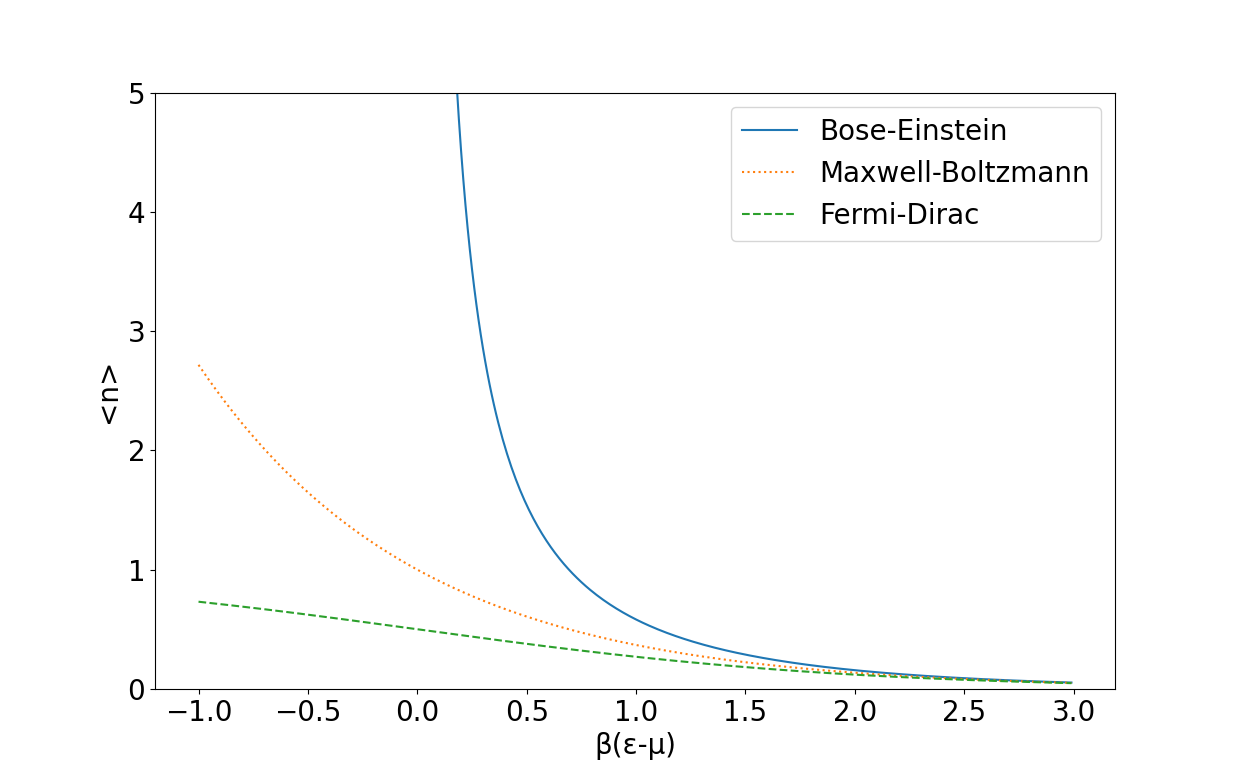
\includegraphics[width=\textwidth]{pic/quantum statistical.png}
    \caption{三种分布}
    \label{quantum statistical}
\end{figure}


\subsection{黑体辐射、凝聚态}
考虑边长为 $ L $ 的正方体盒子中的粒子, 在周期性边界条件下, 粒子的单位特征态为平面波
\[ \psi_k(r)=\left(\frac{1}{L}\right)^{\frac{3}{2}}e^{\mathrm{i}k\cdot r}, \]
其中
\[ k=\left(\begin{matrix}
    k_1\\k_2\\k_3
\end{matrix}\right)=\frac{2\pi}{L}\left(\begin{matrix}
    n_1\\n_2\\n_3
\end{matrix}\right),\quad n_1,n_2,n_3\in\mathbb{Z}. \]
记盒子的体积为 $ V=L^3 $, 则 $ k $ 所在的空间中单位体积对应约 $ V/(8\pi^3) $ 个特征态. 所有特征态对应的 $ k $ 形成了三维空间中的正方格点, 当 $ V $ 很大时, 格点非常密, 可以认为此时 $ k $ 所在的空间中特征态的密度为 $ V/(8\pi^3) $.
\subsubsection*{黑体辐射}
{\bf 黑体辐射}指的是处于平衡态的黑体发出的电磁辐射, 而{\bf 黑体}指的是可以完全吸收外来电磁辐射, 不进行反射和透射的物体. 电磁辐射就是电磁波, 或者从量子角度来看, 电磁辐射是由光子组成的. 光子的速度为光速 $ c $, 频率为 $ \omega=c|k| $, 另外由于电磁波有两个极化方向, 每个波向量 $ k $ 对应两个特征态.

固定温度 $ T $, 一小段频率 $ \mathrm{d}\omega $ 对应的特征态数量 $ g(\omega)\,\mathrm{d}\omega $ 为
\[ g(\omega)\,\mathrm{d}\omega=(4\pi k^2)\left( \frac{\mathrm{d}|k|}{\mathrm{d}\omega}\,\mathrm{d}\omega \right)\left( \frac{2V}{(2\pi)^3} \right), \]
其中等式右侧的第一项是半径为 $ k $ 的球面表面积, 第二项是频率变化 $ \mathrm{d}\omega $ 后半径为 $ k $ 的球面随之变化产生的球壳厚度, 第三项是特征态的密度. 带入 
\[ \frac{\mathrm{d}|k|}{\mathrm{d}\omega}=\frac{1}{c} \] 
可知单位频率对应的特征态数量为
\[ g(\omega)=\frac{V\omega^2}{\pi^2c^3}. \]

光子是玻色子, 化学势为 $ 0 $, 能量和频率的关系为 $ \varepsilon=\hbar\omega $. 根据前文中的结论可得频率 $\omega$ 对应的特征态的光子数 $n_\omega$ 满足
\[ \langle n_\omega\rangle=\frac{1}{e^{\hbar\omega/(k_BT)}-1}, \]
因此每 $ \mathrm{d}\omega $ 频率对应的光子数 $n$ 满足
\[ \langle n\rangle\,\mathrm{d}\omega=\frac{g(\omega)}{e^{\hbar\omega/(k_BT)}-1}\,\mathrm{d}\omega. \]
进一步地, 设 $ u(\omega) $ 为每单位体积的光子能量, 则每 $\mathrm{d}\omega$ 频率对应的能量为
\begin{align*}
    Vu(\omega)\,\mathrm{d}\omega &= \frac{\hbar\omega g(\omega)}{e^{\hbar\omega/(k_BT)}-1}\,\mathrm{d}\omega\\ 
    &=\frac{V\hbar}{\pi^2c^3}\frac{\omega^3\,\mathrm{d}\omega}{e^{\hbar\omega/(k_BT)}-1},
\end{align*}
这就是{\bf 普朗克黑体辐射定律} (Planck's law). 当频率很低时, 作近似 
\[ e^{\hbar\omega/(k_BT)}-1\approx\frac{\hbar\omega}{k_BT} \]
可以得到{\bf 瑞利-金斯定律} (Rayleigh-Jeans law)
\[ u(\omega)\,\mathrm{d}\omega= \left(\frac{k_BT}{\pi^2c^3}\right)\omega^2\,\mathrm{d}\omega. \]

\subsubsection*{凝聚态}
若盒子中有大量质量为 $ m $ 的全同玻色子, 由于 $ p=\hbar k $, 动量空间中特征态个数的密度为 $ V/(2\pi\hbar)^3 $. 单个粒子的能量为 $ \varepsilon=p^2/(2m) $, 且
\[ \frac{\mathrm{d}\varepsilon}{\mathrm{d}|p|}=\frac{|p|}{m}=\sqrt{\frac{2\varepsilon}{m}}, \]
因此每 $ \mathrm{d}\varepsilon $ 能量对应的特征态的数量为
\[ g(\varepsilon)\,\mathrm{d}\varepsilon=(4\pi p^2)\left( \frac{\mathrm{d}|p|}{\mathrm{d}\varepsilon}\,\mathrm{d}\varepsilon \right)\left( \frac{V}{(2\pi\hbar)^3} \right)=\frac{Vm^{\frac{3}{2}}}{\sqrt{2}\pi^2\hbar^3}\sqrt{\varepsilon}\,\mathrm{d}\varepsilon. \]

类似于一份电磁波能量 ($ \hbar\omega $) 对应一个光子, 设化学势为 $ \mu $, 根据玻色-爱因斯坦分布可知此时``总粒子数''为
\[ N(\mu)=\int_{0}^{\infty}\frac{g(\varepsilon)}{e^{(\varepsilon-\mu)/(k_BT)}-1}\,\mathrm{d}\varepsilon. \]
玻色子的化学势一定小于粒子最低的能量, 因此总是有 $ \mu<0 $. 我们可以通过提升化学势来使粒子被分配到每一个特征态中, 其极限状态为 $ \mu=0 $, 此时 $ N $ 达到最大值
\begin{align*}
    N_{\mathrm{max}} &= \int_0^\infty\frac{g(\varepsilon)}{e^{\varepsilon/(k_BT)}-1}\,\mathrm{d}\varepsilon\\ 
    &= \frac{Vm^{\frac{3}{2}}}{\sqrt{2}\pi^2\hbar^3}\int_{o}^{\infty}\frac{\sqrt{\varepsilon}}{e^{\varepsilon/(k_BT)}-1}\,\mathrm{d}\varepsilon\\ 
    &=V\left( \frac{\sqrt{2\pi mk_BT}}{h} \right)^3\frac{2}{\sqrt{\pi}}\int_{\sqrt{z}}^{e^z-1}\,\mathrm{d}z\\ 
    &=\left( \frac{V}{\lambda^3} \right)\zeta\left( \frac{3}{2} \right).
\end{align*}
因此盒子中所允许的最大``粒子密度''为
\[ \frac{N_{\mathrm{max}}}{V}=\frac{\zeta\left( \frac{3}{2} \right)}{\lambda^3}\approx\frac{2.612}{\lambda^3}. \]
假设``粒子数''已达最大值, 但我们还是继续往盒子中塞进新的粒子, 那么多出来的粒子都会被迫处于基态 (能量最低的特征态), 如果我们再继续加入大量的粒子, 那么大部分粒子都会处于基态, 这就是{\bf 玻色-爱因斯坦凝聚态} (Bose-Einstein condensation). 由全同粒子假设知, 这些处于基态的粒子们不可被区分, 换句话说, 它们的行为``整齐划一'', 进而诱发了超流、超导等现象.

另外, 我们也可以固定 $ N $ 和 $ V $, 不断降低温度, 当温度低至
\[ \frac{h^2}{2\pi mk_B}\left( \frac{N}{V\zeta\left( \frac{3}{2} \right)} \right)^{\frac{2}{3}} \]
时也会出现玻色-爱因斯坦凝聚态.

\chapter{电动力学}
经典的电动力学 (或经典电磁学) 研究的是 (真空中的) {\bf 麦克斯韦方程}
\begin{align*}
    \nabla\cdot E&=\frac{\rho}{\varepsilon_0}, \tag{高斯定理}\\
    \nabla\cdot B&= 0, \tag{高斯磁定律}\\ 
    \nabla\times E&=-\frac{\partial B}{\partial t}, \tag{法拉第电磁感应定律}\\
    \nabla\times B&=\mu_0 J+\mu_0\varepsilon_0\frac{\partial E}{\partial t}. \tag{麦克斯韦-安培定律}
\end{align*}
其中 $ E $ 是电场, $ B $ 是磁场, $ \rho $ 是电荷密度, $ \varepsilon_0\approx 8.854187817\times 10^{-12}\text{A}^2\cdot\text{s}^4\cdot\text{kg}^{-1}\cdot\text{m}^{-3} $ 是真空电容率, $ \mu_0\approx 1.2566370614\times 10^{-6} \text{N}\cdot\text{A}^{-2} $ 是真空磁导率, $ J $ 是电流密度.

其中高斯定律描述了电荷如何产生电场, 高斯磁定律指出磁场是无源场 (即不存在磁单极子), 法拉第电磁感应定律描述了磁生电, 麦克斯韦-安培定律描述了电生磁.

若不存在源电流 ($J=0$) 与源电荷 ($\rho=0$), 则麦克斯韦方程组为
\begin{align*}
    \nabla\cdot E&=0,\\
    \nabla\cdot B&=0,\\ 
    \nabla\times E&=-\frac{\partial B}{\partial t},\\
    \nabla\times B&=\mu_0\varepsilon_0\frac{\partial E}{\partial t}.
\end{align*}
对后两个式子取旋度, 可得
\begin{align*}
    \nabla\times(\nabla\times E) &= -\frac{\partial}{\partial t}(\nabla\times B)=-\mu_0\varepsilon_0\frac{\partial^2 E}{\partial t^2},\\ 
    \nabla\times(\nabla\times B) &= \mu_0\varepsilon_0\frac{\partial}{\partial t}(\nabla\times E)=-\mu_0\varepsilon_0\frac{\partial^2 B}{\partial t^2}.
\end{align*}
应用恒等式
\[ \nabla\times(\nabla\times A)=\nabla(\nabla\cdot A)-\nabla^2 A \]
可进一步得到
\[ \begin{aligned}
    \left( \nabla^2-\mu_0\varepsilon_0\frac{\partial^2}{\partial t^2} \right)E &=0,\\ 
    \left( \nabla^2-\mu_0\varepsilon_0\frac{\partial^2}{\partial t^2} \right)B &=0.
\end{aligned} \]
这个方程叫做{\bf 亥姆霍兹方程} (Helmholtz equation), 将其与波动方程
\[ \frac{\partial^2 u}{\partial t^2}=c^2\nabla^2 u \]
(其中 $ c $ 代表波的传播速率) 进行对照可知此时的电和磁形如传播速率为
\[ c=\frac{1}{\sqrt{\mu_0\varepsilon_0}}\approx 299\ 792\ 458 \text{ m/s} \] 
的波 (电磁波). 但这也导致了一个``问题'': 由于麦克斯韦方程组在所有惯性坐标系中的形式都是一样的, 因此通过上述方式推导出的电磁波的传播速率在所有惯性系中也都相同, 这与人们经典物理学中对速度的认知相违背, 这一矛盾后来催生出了狭义相对论.

因此, 本章主要介绍狭义相对论. 
\begin{remark}
本章所涉及的数学前置知识见附录 \ref{differential geometry}, 其中有几点需要特殊强调:
\begin{enumerate}
    \item 度量可以不是正定的 (定义 \ref{metric});
    \item 记号说明见附录 \S\, \ref{notation}.
\end{enumerate}
\end{remark}

\section{相对论基础概念}
狭义相对论的基本假设有两条:
\begin{enumerate}
    \item {\bf 光速不变原理}: 在所有惯性系中真空光速都为 $ c $ (今后若无特殊声明, 均采用几何单位制 $ c=1 $).
    \item {\bf 狭义相对性原理}: 所有惯性系平权, 即所有惯性系中物理定律的表达形式相同.
\end{enumerate}
\subsection{时空}
很自然地, 我们可以认为每一事件都发生在空间的一点 $ x $ 和时间的一瞬 $ t $, 于是我们也反过来称 $ (x,t) $ 为一个{\bf 事件} (event). 全部事件构成的集合叫做{\bf 时空} (spacetime), 一般我们假定时空是一个 $ 4 $ 维流形.

有线性代数的知识, 对于任意有限维线性空间 $ V $ 上的任意度量 $ g $, 必存在一组正交归一基, 使得 $ g $ 在这组基上的表示为对角阵, 且对角元的正负个数 (正负惯性指数) 与基的选取无关. 我们称正惯性指数减去负惯性指数所得结果为{\bf 号差} (signature).

用正交归一基将度量表示为对角矩阵后, 称对角元全为 $ +1 $ 的度量为{\bf 正定度量}或{\bf 黎曼度量} (Riemannian metric), 称恰好有一个对角元为 $ -1 $, 其余对角元均为 $ +1 $ 的度量为{\bf 洛伦兹度量} (Lorentzian metric).

\begin{remark}
    也有资料将洛伦兹度量定义为只有一个对角元为 $ +1 $, 其余对角元均为 $-1$ 的度量, 在本书的量子场论章节, 将会采用这种定义.
\end{remark}

\begin{enumerate}
    \item 经典物理假定时空流形为 $ \mathbb{R}^4 $, 其上配有正定度量. 设 $ \{x^\alpha\} $ 为 $ \mathbb{R}^n $ 的坐标, 则张量场 $ \delta:=\delta_{\alpha\beta}\,\mathrm{d}x^\alpha\otimes\mathrm{d}x^\beta $ 叫做{\bf 欧氏度量}, 二元组 $ (\mathbb{R}^n,\delta) $ 叫做{\bf 欧式空间}或{\bf 欧式时空}, 其中
    \[ \delta_{\alpha\beta}=\begin{cases}
        0, & \alpha\neq\beta,\\ +1, & \alpha=\beta.
    \end{cases} \]
    \item 狭义相对论也假定时空流形为 $ \mathbb{R}^4 $, 但其上配有洛伦兹度量. 设 $ \{x^\alpha\} $ 为 $ \mathbb{R}^n $ 的坐标, 则张量场 $ \eta:=\eta_{\alpha\beta}\,\mathrm{d}x^\alpha\otimes\mathrm{d}x^\beta $ 叫做{\bf 闵氏度量} (Minkowski metric), 二元组 $ (\mathbb{R}^n,\eta) $ 叫做{\bf 闵式空间}或{\bf 闵氏时空}, 其中
    \[ \eta_{\alpha\beta}=\begin{cases}
        0, & \alpha\neq\beta,\\ -1, & \alpha=\beta=0,\\ +1, & \alpha=\beta=1,\dots,n-1.
    \end{cases} \]
    \item 广义相对论允许时空流形为任意 $ 4 $ 维连通流形, 其上配有洛伦兹度量. 这样的流形叫做{\bf 伪黎曼流形}或{\bf 伪黎曼时空}.
\end{enumerate}

狭义相对论研究的就是 $ 4 $ 维闵氏时空的几何. 由 $\eta_{\alpha\beta}$ 的值来看, 第一个坐标分量是特殊的. 实际上, 我们总是用第一个坐标分量来表示时间, 因此, 我们对于张量的指标做以下约定:
\begin{itemize}
    \item 用希腊字母 $\alpha,\beta,\mu,\nu,\dots$ 来表示可以取 $0,1,2,3$ 的指标;
    \item 用从 $ i $ 开始的字母 $ i,j,k,\dots $ 来表示只能取 $1,2,3$ 的指标.
\end{itemize}

给定坐标系 $\{x^\alpha\}$, 借由 $\eta$ 来升降指标, 容易验证
\begin{align*}
    v^0 &=v(\mathrm{d}x^0)=v^\alpha(\mathrm{d}x^0)_{\alpha}\\
    &=\eta^{\alpha\beta}v_{\beta}(\mathrm{d}x^0)_{\alpha}=\eta^{00}v_{0}(\mathrm{d}x^0)_{0}=-v_0.
\end{align*}
类似地有 $v^i=v_i$ (其他类型张量的情况也类似). 因此, 指标 $0$ 的升降会导致一个负号, 而指标 $1,2,3$ 的升降不改变系数的值.

\subsection{光速不变原理}
\label{line element}
\begin{definition}
    给定线性空间 $ V $ 上的洛伦兹度量 $ g $, 我们将 $ V $ 中的向量分为三类:
    \begin{enumerate}
        \item 满足 $ g(v,v)<0 $ 的 $ v $ 叫做{\bf 类时向量} (timelike vector);
        \item 满足 $ g(v,v)=0 $ 的 $ v $ 叫做{\bf 类光向量} (lightlike vector);
        \item 满足 $ g(v,v)>0 $ 的 $ v $ 叫做{\bf 类空向量} (spacelike vector).
    \end{enumerate}
\end{definition}

\begin{definition}[曲线长度]
    对于配有洛伦兹度量 $ g $ 的流形 $ M $, 若其上的 $ C^1 $ 曲线 $ C(t) $ 的每一点的切向量都类时, 则称其为类时曲线, 类似地可以定义类光曲线和类空曲线. 进一步地, 定义这三种曲线从 $ t_1 $ 到 $ t_2 $ 的{\bf 长度}为
    \[ l:=\int_{t_1}^{t_2}\sqrt{|g(T,T)|}\,\mathrm{d}t,\quad T=\frac{\mathrm{d} C(t)}{\mathrm{d} t}. \]
\end{definition}

\begin{remark}
    我们只对这三种曲线定义了长度, 且类光曲线的长度恒为 $ 0 $.
\end{remark}
设曲线 $C(t)$ 在坐标系 $\{x^\alpha\}$ 下的参数表达为 $(x^\alpha(t))$, 则
\[ g(T,T)=g\left( T^\alpha\frac{\partial}{\partial x^\alpha},T^\beta\frac{\partial}{\partial x^\beta} \right)=T^\alpha T^\beta g\left( \frac{\partial}{\partial x^\alpha},\frac{\partial}{\partial x^\beta} \right)=\frac{\mathrm{d}x^\alpha}{\mathrm{d}t}\frac{\mathrm{d}x^\beta}{\mathrm{d}t}g_{\alpha\beta}, \]
因此曲线长度可表达为
\[ l=\int_{t_1}^{t_2}\sqrt{g_{\alpha\beta}\frac{\mathrm{d} x^\alpha}{\mathrm{d} t}\frac{\mathrm{d} x^\beta}{\mathrm{d} t}}\,\mathrm{d} t. \] 
为了方便书写我们还可以引入{\bf 线元} (line element) 记号 
\[ \mathrm{d}s^2:=g_{\alpha\beta}\,\mathrm{d}x^\alpha\mathrm{d}x^\beta. \] 
\begin{remark}
    这里我们记 $\mathrm{d}x^{\alpha}\mathrm{d}x^{\beta}:=\mathrm{d}x^{\alpha}\otimes\mathrm{d}x^{\beta}$, 因此线元只是度量的另一种写法. 
\end{remark}

在洛伦兹坐标系下, 线元为
\[ \mathrm{d}s^2=-(\mathrm{d}x^0)^2+(\mathrm{d}x^1)^2+(\mathrm{d}x^2)^2+(\mathrm{d}x^3)^2. \]
由于我们用第一个坐标分量 $ x^0 $ 来表示时间, 因此也将坐标系 $ \{x^0,x^1,x^2,x^3\} $ 写作 $ \{t,x,y,z\} $, 此时线元为
\[ \mathrm{d}s^2=-\mathrm{d}t^2+\mathrm{d}x^2+\mathrm{d}y^2+\mathrm{d}z^2. \]

质点是牛顿力学中的概念, 指的是空间中带有质量的点, 这里我们将其推广为{\bf 粒子} (particle) 概念, 粒子分为两种: 
\begin{enumerate}
    \item 有 (静) 质量的粒子, 也叫作{\bf 质点}.
    \item 无 (静) 质量的粒子, 也叫做{\bf 光子}(photon).
\end{enumerate}
一个粒子的全部历史由一系列事件组成, 对应时空中的一条曲线, 该曲线叫做该粒子的{\bf 世界线} (world line). 

给定一个粒子的世界线 $ (t,x(t),y(t),z(t)) $, 我们熟知的速率可定义为
\[ v:=\frac{\sqrt{\mathrm{d}x^2+\mathrm{d}y^2+\mathrm{d}z^2}}{\mathrm{d}t}, \]
上式可改写为
\[ \mathrm{d}s^2=-(1-v^2)\,\mathrm{d}t^2. \]
这说明狭义相对论中的两个假设
\begin{enumerate}
    \item (光速不变原理) 光子相对于任意惯性系的速率为 $ 1 $.
    \item 质点相对于任意惯性系的速率小于光速 $ 1 $.
\end{enumerate}
可被重新表述为下面两个公理 (暂时忽略惯性系概念):
\begin{enumerate}
    \item 光子世界线为类光曲线 ($ \mathrm{d}s^2=0 $).
    \item 质点世界线为类时曲线 ($ \mathrm{d}s^2<0 $).
\end{enumerate}

\subsection{狭义相对性原理}
我们将进行物理观测的人视为质点, 称其为{\bf 观者} (observer), 观者手中有一个{\bf 标准钟} (standard clock), 该钟的读数叫做该观者的{\bf 固有时} (proper time), 一个观者的固有时是该观者自身所经历的时间. 而每点的第一个坐标分量叫做该坐标系下的{\bf 坐标时} (coordinate time).

\begin{remark}
    严谨地说, 观者是配有正交归一标架场的类时曲线.
\end{remark}

\begin{definition}[标准钟]
    若一个钟在自己世界线上任意两点 $ p_1,p_2 $ 的读数 $ \tau_1,\tau_2 $ 之差为 $ p_1,p_2 $ 之间的线长, 则我们称它为{\bf 标准钟}或{\bf 理想钟} (ideal clock).
\end{definition}

\begin{remark}
    今后谈及世界线时默认以固有时 $ \tau $ 为参数, 由于固有时等于线长, 其切向量的长度为 $ 1 $. 
\end{remark}

推而广之, 我们可以认为每个质点都是一个观者, 有自己的固有时. 但光子没有固有时, 不能充当观者.

如果一个由观者构成的集合 $ \mathcal{R} $ 满足时空 (或其中任意开子集) 中每一点恰有 $ \mathcal{R} $ 内的一个观者的世界线经过, 则称 $ \mathcal{R} $ 为一个 (局部) {\bf 参考系} (reference frame). 

想象每个观者带有一个标准钟, 其读数为 $ t $, 且身上标有三个实数 $ (x,y,z) $, 则任一事件必发生在某一观者身上, 它可以记录下该事件的时空坐标 $ \{t,x,y,z\} $. 有时我们也反过来用坐标 $\{t,x,y,z\}$ 来代指相应的参考系.

狭义相对性原理指出存在一类特殊的观者是惯性 (inertial) 观者, 且它们相互之间平权, 不存在特殊的惯性观者, 比如不能说哪个惯性观者是绝对静止的. 一族惯性观者构成的参考系叫做惯性参考系.

若一个质点的世界线为测地线 (定义 \ref{geodesic}), 则称该质点为``自由的''或``做惯性运动的'', 其对应的观者叫做{\bf 惯性观者}. 由惯性观者构成的参考系叫做{\bf 惯性参考系}, 属于同一惯性参考系的所有观者的世界线是相互平行的测地线. 以观者的固有时作为 $ t $ 坐标所得到的坐标系叫做{\bf 惯性坐标系}. 在不需要区分参考系和坐标系时, 我们将惯性参考系和惯性坐标系统称为{\bf 惯性系}. 
\begin{remark}
    严谨地说, 惯性观者是做惯性运动的无自转观者 (详见 \S\,\ref{rotation}). 在狭义相对论中, 与惯性系坐标 $\{t,x,y,z\}$ 对应的标架
    \[ \left\{\frac{\partial}{\partial t},\,\frac{\partial}{\partial x},\,\frac{\partial}{\partial y},\,\frac{\partial}{\partial z}\right\}, \]
    能保证观者是无自转的, 因此不用担心这个问题.
\end{remark}
定义{\bf 洛伦兹系}为闵氏时空中满足
\[ \eta\left( \frac{\partial}{\partial x^\alpha},\frac{\partial}{\partial x^\beta} \right)=\eta_{\alpha\beta} \]
的坐标系 $ \{x^0,x^1,x^2,x^3\} $. 于是洛伦兹系之间的变换对应于 $ (\mathbb{R}^4,\eta) $ 中的等距微分同胚 \cite[定理 4-3-6]{梁灿彬2000微分几何入门与广义相对论}, 而任一等距微分同胚可由以下几类基本的等距微分同胚复合而成 \cite[上册 136 页]{梁灿彬2000微分几何入门与广义相对论}:
\begin{enumerate}
    \item 空间反射, 如 $ x'= -x $.
    \item 时间反演 $ t'=-t $.
    \item 平移, 如 $ t'=t+a $ 和 $ x'=x+a $.
    \item 空间旋转, 如 $\ \begin{aligned}
            x'&=x\cos\theta-y\sin\theta,\\
            y'&=x\sin\theta+y\cos\theta.
    \end{aligned}$
    \item {\bf 洛伦兹变换}, 如 $\ \begin{aligned}
        t'&=t\cosh\alpha-x\sinh\alpha,\\
        x'&=-t\sinh\alpha+x\cosh\alpha.
    \end{aligned}$.
\end{enumerate}

第一类变换会改变手性, 第二类变换会改变时间方向, 它们都是在重新设定坐标轴方向, 我们不关心这些变换, 以后不再讨论它们. 后三类变换是我们所关心的, 实际上, 后三类变换所生成的洛伦兹系 (即保持时间方向和手性的等距微分同胚所对应的坐标系) 恰是惯性系; 反之, 惯性系也都是这样的洛伦兹系.
\begin{remark}
    因此惯性系可以视作所有坐标系商掉一个等价关系后的一个等价类, 这是狭义相对性原理的数学体现. 注意 $\mathbb{R}^4$ 自然拥有的坐标系显然是惯性系, 因此我们已经先钦定了一个惯性系等价类的代表元.
\end{remark}
接下来讨论后三类变换. 平移是在重新设置初始值 (原点), 空间旋转是在重新设置 $x,y,z$ 轴的方向. 对于洛伦兹变换, 我们也将其写作 
\begin{align*}
    t' &= \gamma\left(t-\frac{vx}{c^2}\right),\\ 
    x' &= \gamma(x-vt),
\end{align*}
其中
\[ \gamma:=\frac{1}{\sqrt{1-\frac{v^2}{c^2}}} \] 
叫做{\bf 洛伦兹因子}. 这对应于两个惯性系 $ \mathcal{R}' $ 和 $ \mathcal{R} $ 之间的坐标变换, 两个坐标系的坐标轴分别平行且朝向相同, $ \mathcal{R}' $ 相对与 $ \mathcal{R} $ 以速率 $ v $ 沿 $ x $ 轴正向匀速移动. 若定义{\bf 快度}(rapidity)为 
\[ \alpha=\mathrm{arctanh}\left( \frac{v}{c} \right),\] 
则 $\gamma=\cosh\alpha$ 且洛伦兹变换可写为
\[ \left(\begin{matrix}
   ct' \\ x' 
\end{matrix}\right)=\left(\begin{matrix}
    \cosh\alpha & -\sinh\alpha\\ 
    -\sinh\alpha & \cosh\alpha
\end{matrix}\right)\left(\begin{matrix}
    ct \\ x
\end{matrix}\right), \]
这就是前文给出的双曲函数形式的洛伦兹变换, 其逆变换为
\[ \left(\begin{matrix}
    ct \\ x
\end{matrix}\right)=\left(\begin{matrix}
    \cosh\alpha & \sinh\alpha\\ 
    \sinh\alpha & \cosh\alpha
\end{matrix}\right)\left(\begin{matrix}
    ct' \\ x'
\end{matrix}\right). \]

\begin{figure}[H]
    \centering
    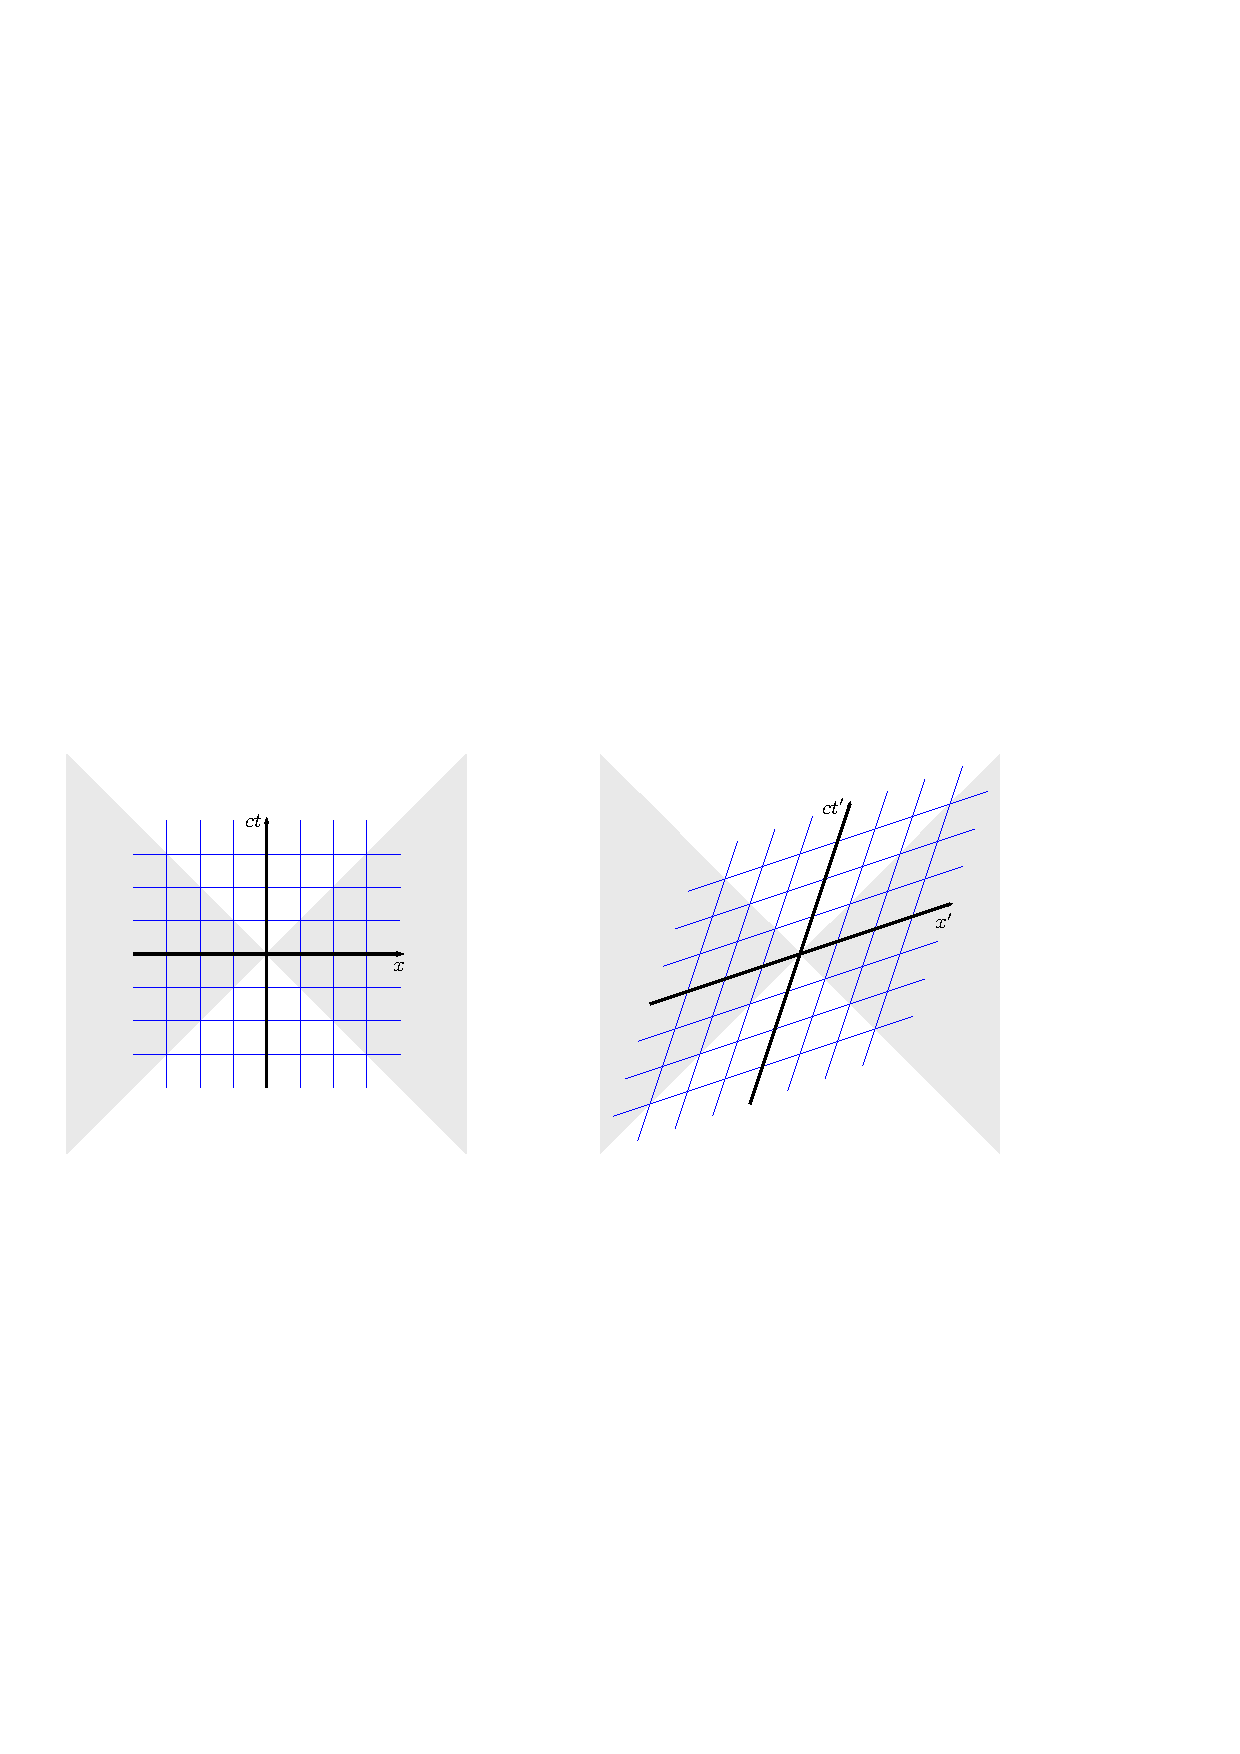
\includegraphics[width=0.85\textwidth]{pic/Lorentz transform.pdf}
    \caption{Lorentz transform}
    \label{Lorentz transform}
\end{figure}

以牛顿力学的角度来看, 不能超光速略显奇怪; 如今在狭义相对论中, 速度不能叠加, 但由    
\[ \left(\begin{matrix}
    \cosh\alpha_1 & \sinh\alpha_1\\ 
    \sinh\alpha_1 & \cosh\alpha_1
\end{matrix}\right)\left(\begin{matrix}
    \cosh\alpha_2 & \sinh\alpha_2\\ 
    \sinh\alpha_2 & \cosh\alpha_2
\end{matrix}\right)=\left(\begin{matrix}
    \cosh(\alpha_1+\alpha_2) & \sinh(\alpha_1+\alpha_2)\\ 
    \sinh(\alpha_1+\alpha_2) & \cosh(\alpha_1+\alpha_2)
\end{matrix}\right) \] 
知同一方向上的快度是可以叠加的, 若利用快度来进行思考, 由 $\mathrm{arctanh}$ 的图像知光速对应着 $\infty$ 快度, 这显然不能被超越的, 甚至是无法达到的.
\section{典型效应}
这一节中我们用 $ l $ 来表示线长.
\subsection{钟慢效应}
考虑两个在惯性系 $ \mathcal{R} $ 中静止的标准钟 $ C_1 $, $ C_2 $ 和一个在惯性系 $ \mathcal{R}' $ 中的静止的标准钟 $ C' $, 它们的世界线如图 \ref{time dilation} 所示.

\begin{figure}[htbp]
    \centering
    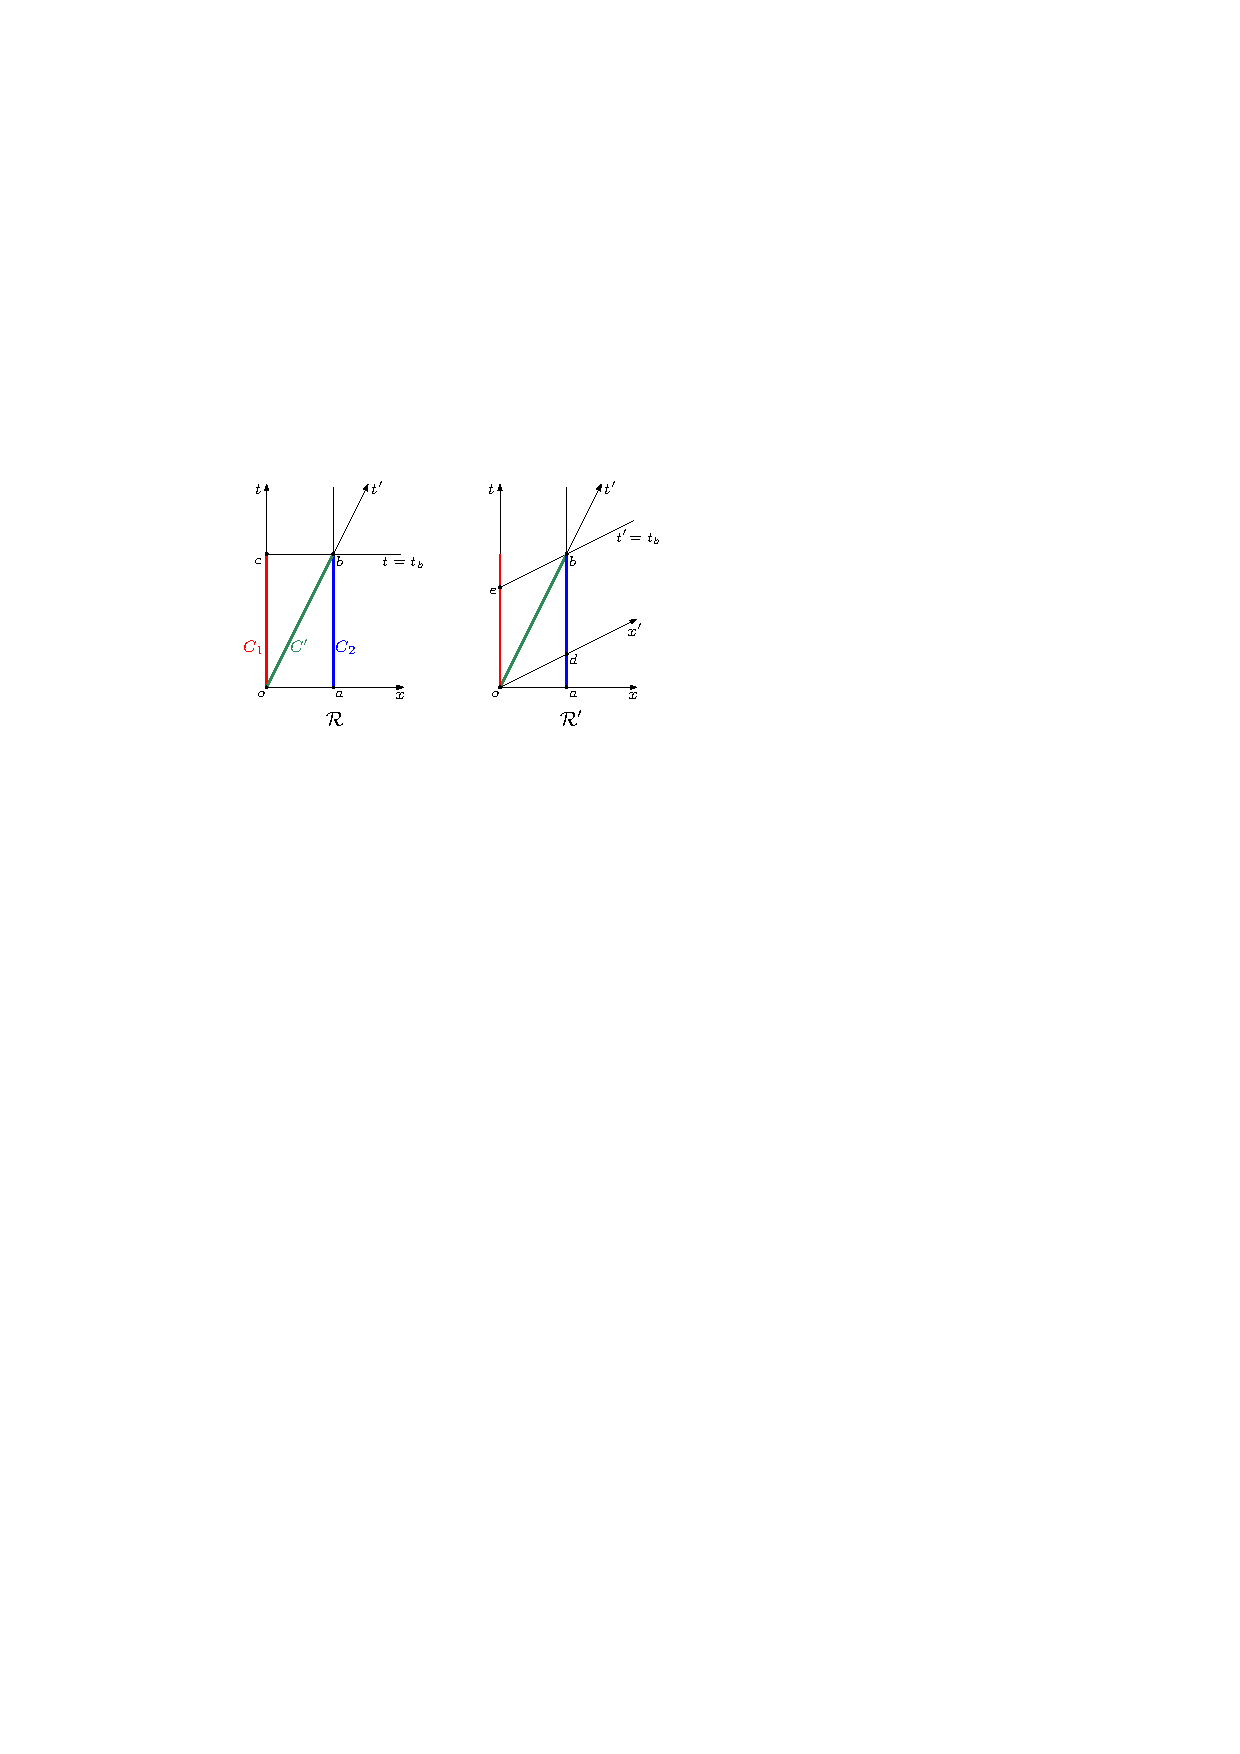
\includegraphics[width=0.8\textwidth]{pic/time dilation.pdf}
    \caption{time dilation}
    \label{time dilation}
\end{figure}

先在 $ \mathcal{R} $ 系的视角中进行讨论, 当 $ t=0 $ 时我们将三个钟的读数都调为 $ 0 $, 此时 $ C' $ 与 $ C_1 $ 重合; 当 $ t=t_b $ 时, $ C' $ 与 $ C_2 $ 重合, 此时 $ C_2 $ 的读数为 $ l_{ab}=t_b$, $ C' $ 的读数为 $ l_{ob}=\sqrt{t_b^2-x_b^2}<l_{ab}$, 因此在 $ \mathcal{R} $ 系看来钟 $ C' $ 走慢了.

\begin{remark}
    上述讨论中有一些细节需要注意:
    \begin{enumerate}
        \item 在一个参考系中, 我们称所有时间分量相同的点所构成的集合为同时面, 语句 ``当 $ t=0 $ 时'' 应理解为语句 ``在 $ t=0 $ 的同时面上'' 的缩写.
        \item 只有在两个钟重合于某一点时才能比较读数, 比如当 $ t=t_b $ 时, $ C' $ 只能和 $ C_2 $ 比较读数, 不能和 $ C_1 $ 比较读数.
        \item 信息的传播需要时间, 若 $ C_1 $ 将自己读数调为 $ 0 $ 的同时告诉 $ C_2 $ 调读数, 那 $ C_2 $ 收到消息并将读数调为 $ 0 $ 时, $ C_1 $ 的读数已经不是 $ 0 $ 了. 钟 $ C_1 $ 和 $ C_2 $ 在 $ t=0 $ 时读数都为 $ 0 $ 这个条件叫做{\bf 钟同步} (clock synchronization), 一个实现钟同步的方法如图 \ref{clock synchronization} 所示: $ C_1 $ 朝 $ C_2 $ 发射一束光并记下自己的读数 $ t_1 $, $ C_2 $ 手持一面镜子将光反射回去, $ C_1 $ 在收到反射回来的光时记下自己的读数 $ t_2 $ 并计算读数差 $ \Delta t=t_1-t_2 $, 接下来 $ C_1 $ 再发射一束光并在自己的读数增加 $ \Delta t/2$ 后将自己的读数调为 $ 0 $, 而 $ C_2 $ 再次接收到光时也将自己的读数调为 $ 0 $. (这一方法利用了光速与方向无关的假设)
    \end{enumerate}
    \begin{figure}[htbp]
        \centering
        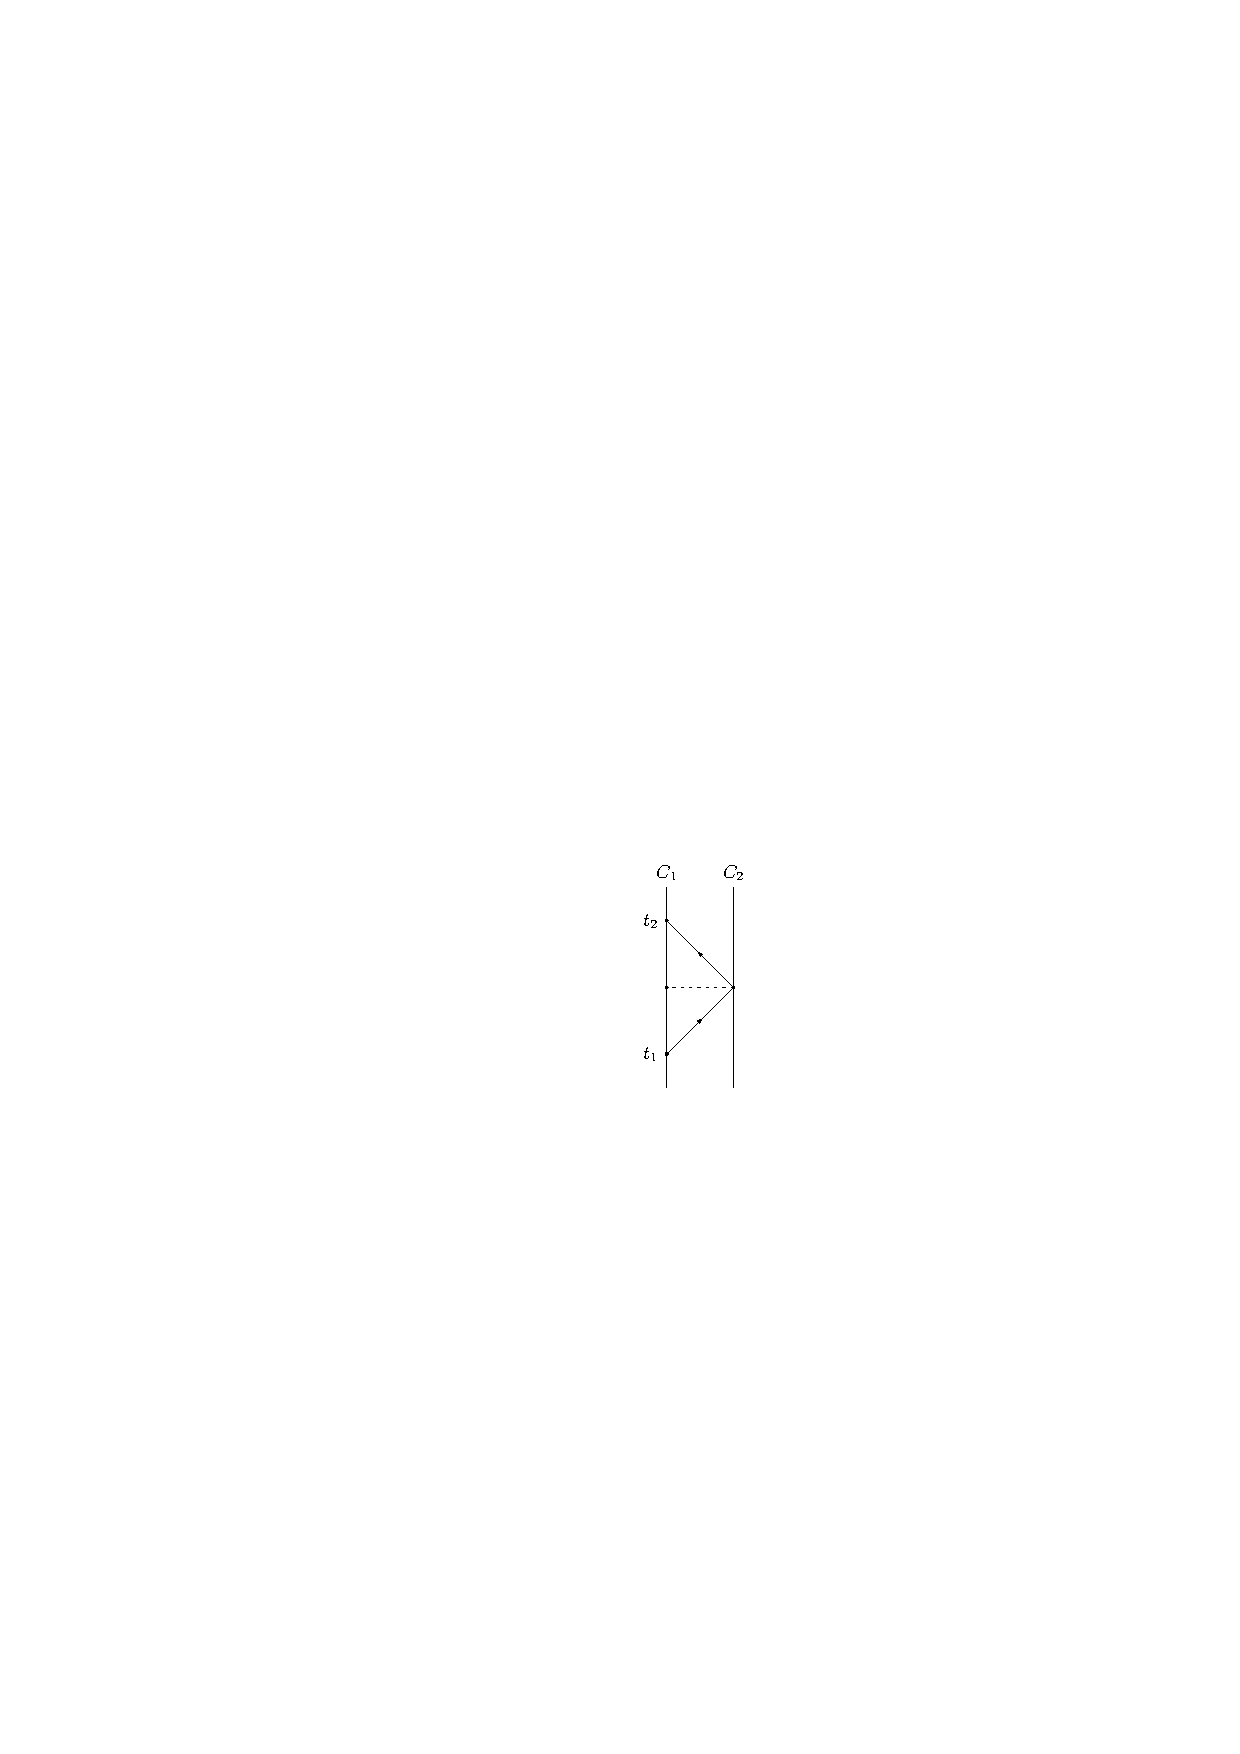
\includegraphics[width=0.2\textwidth]{pic/clock synchronization.pdf}
        \caption{clock synchronization}
        \label{clock synchronization}
    \end{figure}
\end{remark}

在 $ \mathcal{R}' $ 系的视角中, 事件 $ o $ 与 $ d $ 是同时的, 此时 $ C_1 $ 和 $ C' $ 的读数为 $ 0 $, 而 $ C_2 $ 的读数为 $ l_{ad}>0 $, 因此 $ \mathcal{R} $ 系认为 $ C_2 $ 偷跑了一段时间, 在 $ t'=t'_b $ 时应与 $ C' $ 的读数 $ l_{ob}=t'_b $ 作比较的是 $ C_2 $ 在 $ t'=t'_b $ 时和 $ t'=0 $ 时的读数差 $ l_{db}=\sqrt{t'_b{}^2-x'_b{}^2}<l_{ob}$, 这说明在 $ \mathcal{R} $ 系看来钟 $ C_2 $ 慢了.

\begin{remark}
    再次强调, 在同时面 $ t'=0 $ 上, $ C' $ 可以说与其重合的 $ C_1 $ 的读数为 $ 0 $, 但不能说处于点 $ d $ 的 $ C_2 $ 读数怎样. 由此可以看出, 将参考系定义为一族观者构成的集合是非常明智的, 用一族世界线覆盖整个时空, 我们就可以讨论时空中的每一点.
\end{remark}

考虑某个质点的世界线 $ L(\tau) $, 用 $ \tau $ 表示其固有时, 用 $ t $ 表示惯性系 $ \mathcal{R} $ 的坐标时, 则由 $ \mathrm{d}\tau=\sqrt{-\mathrm{d}s^2} $ 和 $ \mathrm{d}s^2=-(1-v^2)\,\mathrm{d}t^2 $ 可知
\[ \frac{\mathrm{d}t}{\mathrm{d}\tau}=\frac{1}{\sqrt{1-v^2}}=\gamma, \]
其中 $ v $ 是该质点相对于 $ \mathcal{R} $ 的速率. 这就是所谓的``动钟变慢''.

\subsection{尺缩效应}
如图 \ref{length contraction} 所示, 阴影部分是一把尺子的世界面, 在尺子所在的惯性系 $ \mathcal{R} $ 看来, 尺子的长度为 $ l_{oa} $, 而在另一个惯性系 $ \mathcal{R'} $ 看来, 尺子的长度为 $ l_{ob}<l_{oa} $, 这就是所谓的``动尺变短''.

产生这种现象的原因在于, 在 $ 4 $ 维时空中, 尺子是一个 $ 2 $ 维的面 (假设它在三维中是 $ 1 $ 维的线), 不同的参考系将不同的线的线长作为尺长, 是在盲人摸象.
\begin{figure}[H]
    \centering
    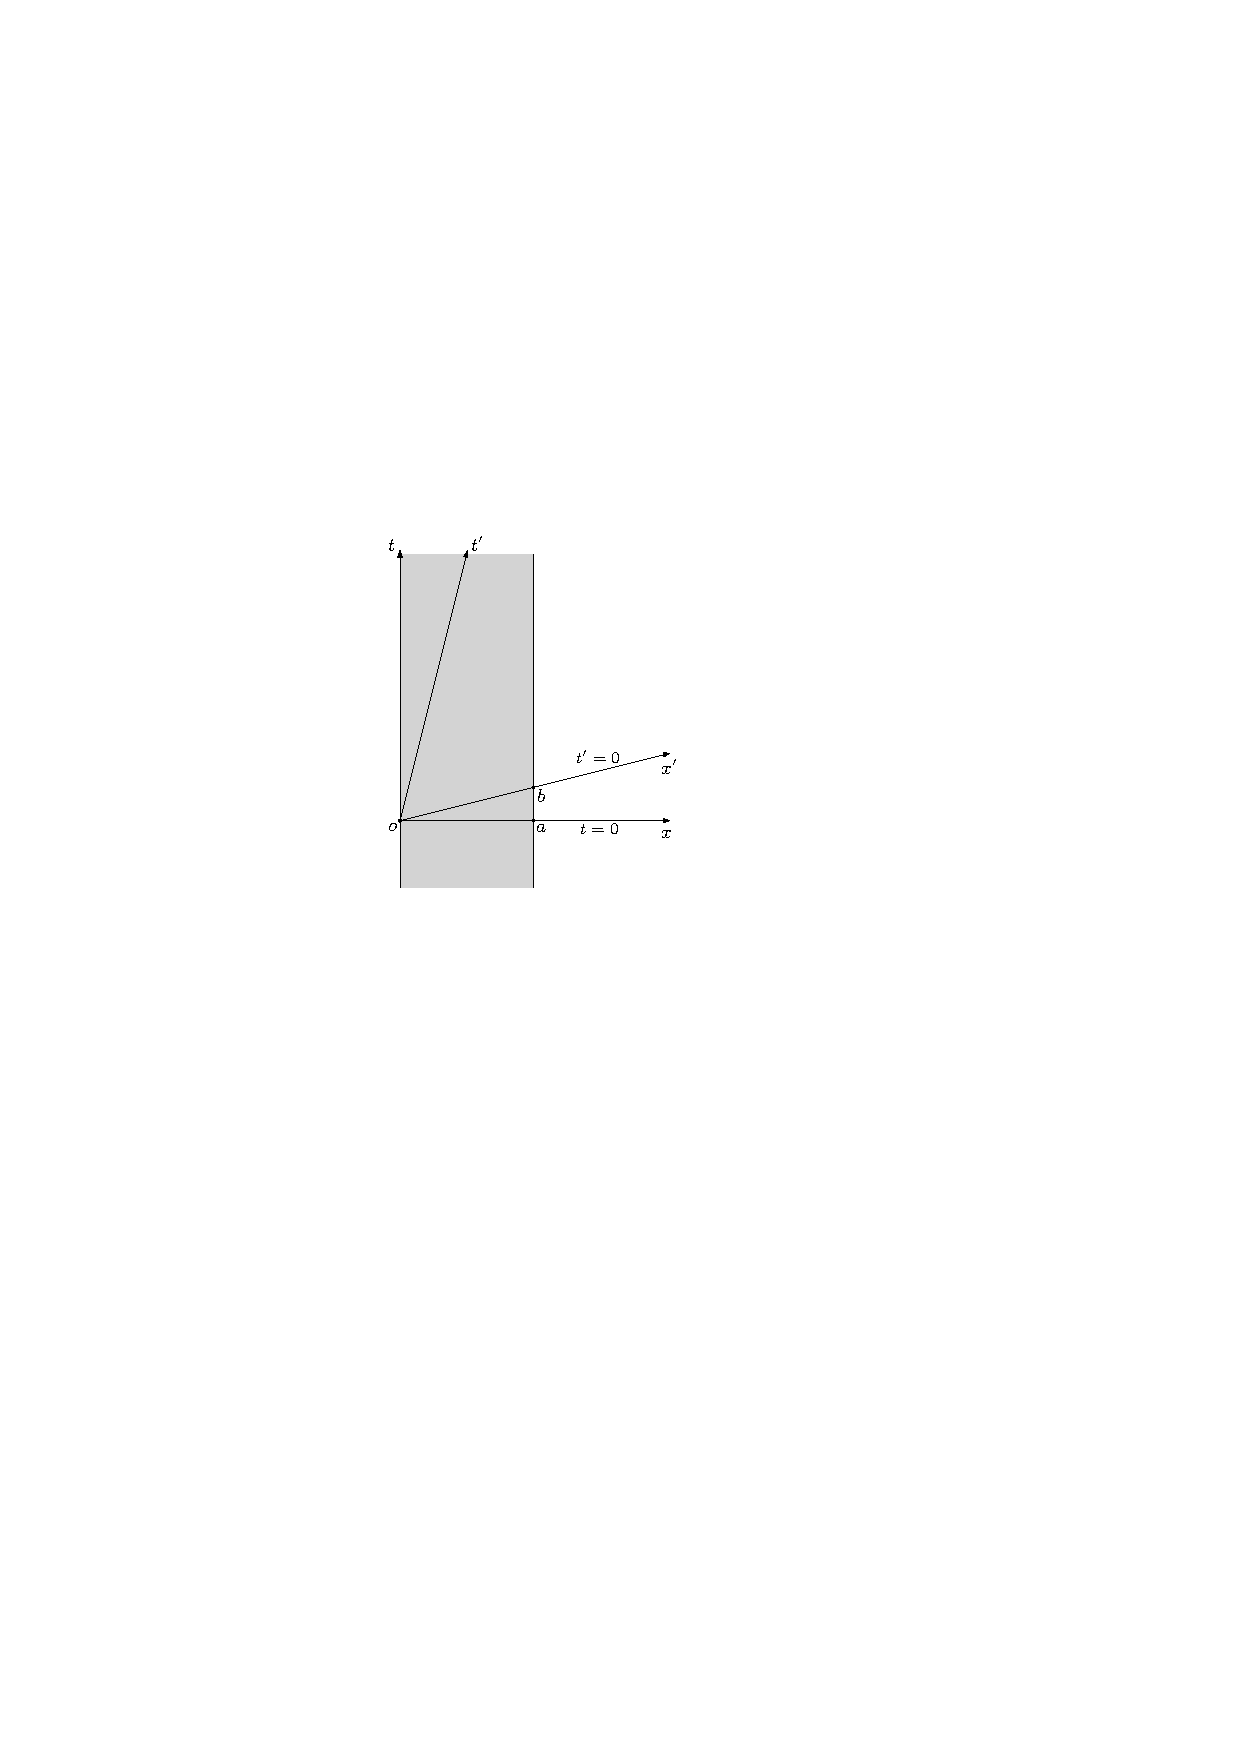
\includegraphics[width=0.4\textwidth]{pic/length contraction.pdf}
    \caption{length contraction}
    \label{length contraction}
\end{figure}

\subsection{双生子佯谬}
如图 \ref{twin paradox} 所示, $ A $ 和 $ B $ 分别以不同的路线从 $ p $ 走到 $ q $, 惯性观者 $ A $ 所经历的时间要小于非惯性观者 $ B $ 所经历的时间.

\begin{figure}[H]
    \centering
    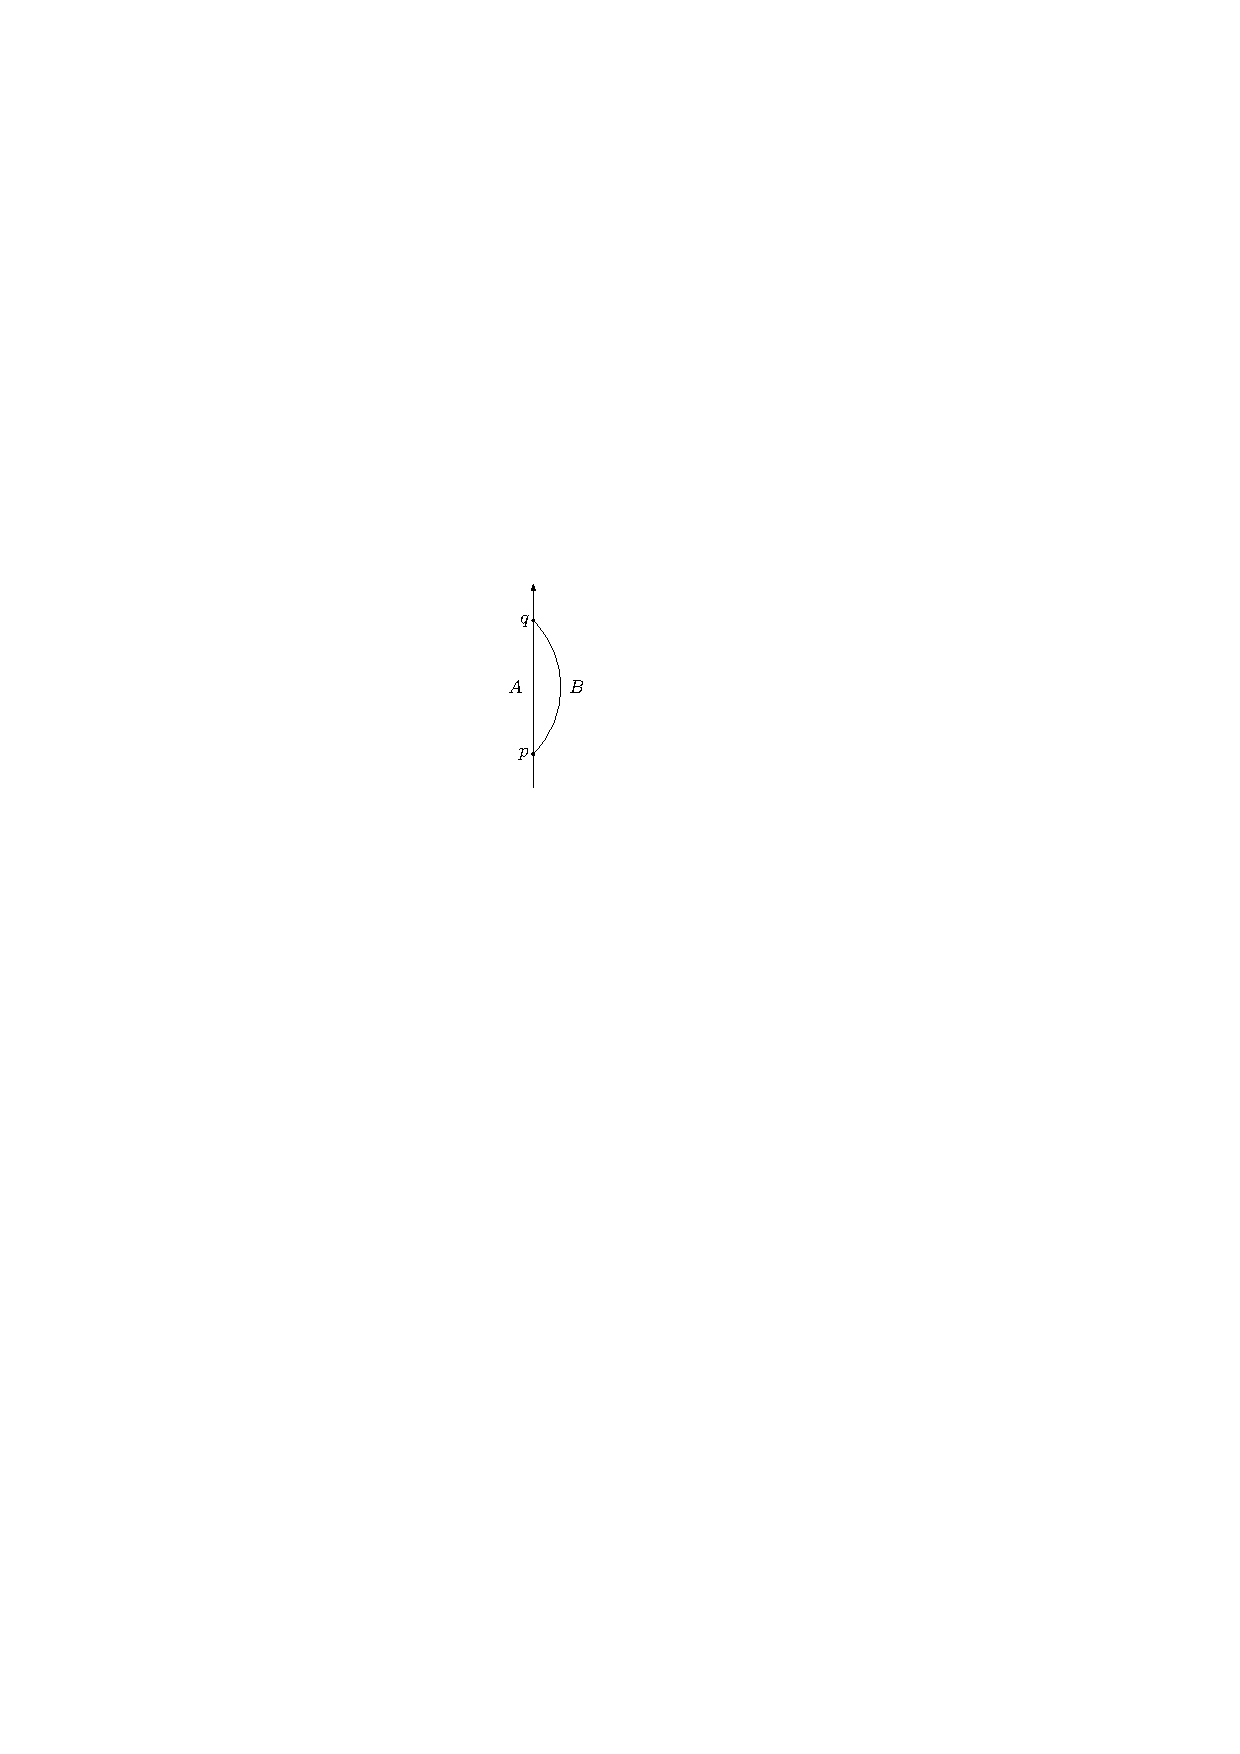
\includegraphics[width=0.2\textwidth]{pic/twin paradox.pdf}
    \caption{twin paradox}
    \label{twin paradox}
\end{figure}

\section{质点}
接下来我们要在 $ 4 $ 维时空中讨论经典运动学中的各种概念 (及其推广).
\subsection{切向量的 \texorpdfstring{$ 3+1 $}{3+1} 分解}
\begin{definition}[$ 4 $ 速度]
    质点的 $ 4 $ {\bf 速度}是质点世界线的切向量
    \[ U:=\frac{\partial}{\partial\tau}. \]
\end{definition}
由于固有时是质点世界线的线长参数, 固有时对应的切向量为单位向量, 即 $ 4 $ 速度满足 $ |\eta_{\alpha\beta}U^\alpha U^\beta|=1 $.

将一点 $ p $, 及 $ p $ 上的一个 (指向未来的) 类时单位向量 $ Z $ 的组合 $ (p,Z) $ 称为一个{\bf 瞬时观者} (instantaneous observer), 其中 $Z$ 是该观者的 $4$ 速度.  
\begin{remark}
    严格地说, 一个瞬时观者应该是一点 $ p $ 及该点处的一个正交归一标架 $ \{e_\alpha\} $, 其中 $ e_0=Z $ 为类时向量. 在不会产生混淆的情况下, 我们省略 $ e_0 $ 之外的基向量. 由于 $Z$ 是标架的一部分, 我们一般不将其记作 $Z^\alpha$.
\end{remark}
\begin{remark}
    任给瞬时观者 $(p,Z)$, 一定存在一个惯性观者, 其世界线过点 $p$, 且世界线在点 $p$ 处的切向量为 $Z$. 因此在不会产生混淆时, 我们也将瞬时观者简称为观者.
\end{remark}

\begin{definition}[切空间的 $3+1$ 分解]
    对于任意观者 $G$ 的世界线上的任意一点 $ p $, 都有一个对应的瞬时观者 $ (p,Z) $, 我们将点 $ p $ 处的切空间做 $ 3+1 $ 分解 $ N_p\oplus S_p $, 其中
    \begin{align*}
        N_p&=\mathrm{span}\{Z\},\\
        S_P&=\left\{ V^{\alpha}\in T_pM \;\middle|\; \eta_{\alpha\beta}V^\alpha Z^\beta=0 \right\}.
    \end{align*}
    我们称 $ S_p $ 中的向量为空间向量 (spatial vector), $ S_p $ 就是 $ G $ 在这一瞬间所感受到的空间. 
\end{definition}

\begin{remark}
    空间向量一定是类空向量, 而反之不然.
\end{remark}

\begin{proposition}
    任给瞬时观者 $(p,Z)$, 点 $ p $ 处度量 $ \eta $ 在 $ S_p $ 上的诱导度量 (将 $ \eta $ 限制到 $ S_p $ 上)  为
    \[ h_{\alpha\beta}=\eta_{\alpha\beta}+Z_{\alpha}Z_{\beta}. \]
\end{proposition}
\begin{proof}
    给定标架 $\{e_\alpha\}$, 其中 $e_0=Z$. 则 
    \[ h_{0\beta}=h_{\alpha\beta}Z^{\alpha}=\eta_{\alpha\beta}Z^\alpha+Z_{\alpha}Z_{\beta}Z^{\alpha}=Z_\beta-Z_\beta=0,\quad \alpha=0,1,2,3. \]
    因此 $h_{\alpha\beta}$ 是定义在 $S_p$ 上的.
    任给 $v^{\alpha},w^{\alpha}\in S_p$, 则
    \[ h_{\alpha\beta}v^{\alpha}w^{\beta}=\eta_{\alpha\beta}v^{\alpha}w^{\beta}+Z_{\alpha} Z_{\beta}v^{\alpha}w^{\beta}=\eta_{\alpha\beta}v^{\alpha}w^{\beta}, \]
    因此 $h_{\alpha\beta}$ 为 $\eta_{\alpha\beta}$ 在 $S_p$ 上的诱导度量.
\end{proof}

\begin{proposition}
    任给瞬时观者 $(p,Z)$ 及点 $p$ 处的切向量 $u^{\alpha}$, 对 $u^{\alpha}$ 做 $3+1$ 分解 $u^{\alpha}=v^{\alpha}+w^{\alpha}$, 其中 $v^{\alpha}\in N_p$, $w^{\alpha}\in S_p$, 则
    \[ v^{\alpha} = -Z^{\alpha}(Z_{\beta}u^{\beta}),\quad
        w^{\alpha} = h^{\alpha}{}_{\beta}u^{\beta}. \]
\end{proposition}
\begin{proof}
    由于
    \[ h^{\alpha}{}_{\beta}=\eta^{\alpha\mu}h_{\mu\beta}=\delta^{\alpha}{}_{\beta}+Z^{\alpha}Z_{\beta}, \]
    我们可将 $u^{\alpha}$ 分解为
    \[ u^{\alpha}=h^{\alpha}{}_{\beta}u^{\beta}-Z^{\alpha}(Z_{\beta}u^{\beta}), \]
    其中 $ -Z^{\alpha}(Z_{\beta}u^{\beta})\in N_p $, 且 $-Z^{\alpha}(Z_{\beta}u^{\beta})Z_\alpha=-Z_{\beta}u^{\beta}$, 因此这就是 $u^{\alpha}$ 到 $N_p$ 上的投影, 进而知 $h^{\alpha}{}_{\beta}u^{\beta}$ 是 $u^{\alpha}$ 到 $S_p$ 上的投影.
\end{proof}

\subsection{质点运动学与动力学}
\textcolor{blue}{再次强调我们只关心惯性系, 以下所有坐标展开都是在惯性系中进行的.}

由于任意空间向量 $v^\alpha$ 的第一个分量为 $0$, 我们也可将其简记为 $v^i$, 有时也将其记为 $\vec{v}$. 下文中所有 $3$ 物理量都是依赖于观者的空间向量, 默认第一个分量为 $0$.

一个质点的 $ 4 $ 速度 $ U $ 可以借由瞬时观者 $ (p,Z) $ 展开为
\[ U=\frac{\partial}{\partial\tau}=\frac{\mathrm{d}t}{\mathrm{d}\tau}\frac{\partial}{\partial t}+\frac{\mathrm{d}x^{i}}{\mathrm{d}\tau}\frac{\partial}{\partial x^i}. \]
于是前文中定义的洛伦兹因子
\[ \gamma=\frac{\mathrm{d}t}{\mathrm{d}\tau}=\frac{1}{\sqrt{1-v^2}}. \]
可重写表达为
\[ \gamma=-U^\alpha Z_\alpha. \]
这是因为
\[ -U^\alpha Z_\alpha=-\eta_{\alpha\beta}U^\alpha\left( \frac{\partial}{\partial t} \right)^{\beta}=-\eta_{00}U^0\left( \frac{\partial}{\partial t} \right)^0=U^0=\frac{\mathrm{d}t}{\mathrm{d}\tau}=\gamma. \]

\begin{definition}[$ 3 $ 速度]
    质点相对于瞬时观者 $ (p,Z) $ 的 $ 3 $ {\bf 速度}为
    \[ u^{i}:=\frac{\mathrm{d}x^i}{\mathrm{d}t}\frac{\partial}{\partial x^{i}}. \]
\end{definition}
\begin{proposition}
    质点的 $ 4 $ 速度可借由瞬时观者 $ (p,Z) $ 做 $ 3+1 $ 分解
    \[ U^{\alpha}=\gamma(Z^{\alpha}+u^{\alpha}). \]
\end{proposition}
\begin{definition}[$ 3 $ 速率]
    质点相对于瞬时观者的 $ 3 $ {\bf 速率}为 $ \sqrt{u^{\alpha}u_{\alpha}}$.
\end{definition}

\begin{definition}[$ 4 $ 动量]
    设质点的 (静) 质量为 $ m $, 则其 $ 4 $ {\bf 动量}为
    \[ P^\alpha:=mU^\alpha. \]
\end{definition}

\begin{definition}[能量与 $ 3 $ 动量]
    质点的 $ 4 $ 动量可借由瞬时观者 $ (p,Z) $ 做 $ 3+1 $ 分解
    \[ P^{\alpha}=m(\gamma Z^{\alpha}+\gamma u^{\alpha})=:EZ^{\alpha}+p^{\alpha}, \]
    我们称其中的 $ E=\gamma m $ 为{\bf 能量}, $ p^{\alpha}=\gamma m u^{\alpha} $ 为 $ 3 $ {\bf 动量}.
\end{definition}

\begin{remark}
    能量是依赖于观者的物理量.
\end{remark}

\begin{proposition}[质能方程]
    记 $ p^2=p^\alpha p_\alpha $, 则
    \[ E^2=m^2+p^2. \]
\end{proposition}
\begin{proof}\keepline
    \begin{align*}
    P^\alpha P_\alpha&=(EZ^\alpha+p^\alpha)(EZ_\alpha+p_\alpha)=-E^2+p^2,\\
        P^\alpha P_\alpha&=mU^\alpha mU_\alpha=-m^2.\qedhere
    \end{align*}
\end{proof}

\begin{remark}
    若不使用几何单位制, 则 $ E^2=m^2c^4+p^2c^2 $. 
\end{remark}

若瞬时观者 $ (p,Z) $ 与被观测质点的世界线相切, 则称 $ (p,Z) $ 为该质点的{\bf 瞬时静止观者}, 瞬时静止观者测得的能量也叫做静能量, 其数值与静质量相同.

\begin{definition}[$ 4 $ 加速度]
    设质点的 $ 4 $ {\bf 加速度}为
    \[ A^\alpha:=U^\beta\partial_\beta U^{\alpha}. \]
\end{definition}

\begin{remark}
    一个观者是惯性的当且仅当其 $4$ 加速度为 $0$.
\end{remark}

\begin{proposition}
    质点世界线上各点处的 $ 4 $ 加速度与 $ 4 $ 速度正交, 即 $ A^\alpha U_\alpha=0$.
\end{proposition}
\begin{proof}\keepline
    \[ A^\alpha U_\alpha=U^\beta(\partial_\beta U^\alpha)U_\alpha=\frac{1}{2}U^\beta\partial_\beta(U^\alpha U_\alpha)=0.\qedhere \]
\end{proof}

\begin{definition}[$ 3 $ 加速度]
    设质点世界线 $ L(\tau) $ 在惯性系 $ \{t,x^i\} $ 中的参数表达式为 $ t=t(\tau) $, $ x^i=x^i(\tau) $, 则它相对于该坐标系的 $ 3 $ {\bf 加速度}为
    \[ a^i:=\frac{\mathrm{d}^2 x^i(t)}{\mathrm{d}t^2}, \]
    其中 $ x^i(t) $ 是 $ x^i=x^i(\tau) $ 与 $ t=t(\tau) $ 的结合.
\end{definition}
\begin{proposition}
    \label{4 force}
    质点的 $ 4 $ 加速度在惯性系中的分量为
    \begin{align*}
        A^0&=\gamma^4(\vec{u}\cdot \vec{a}),\\
        A^i&=\gamma^2a^i+\gamma^4(\vec{u}\cdot \vec{a})u^i,
    \end{align*}
    其中 $ \vec{u} $ 和 $ \vec{a} $ 为 $ 3 $ 速度和 $ 3 $ 加速度, $ \cdot $ 为欧式内积.
\end{proposition}
\begin{remark}
    自由质点相对于任意惯性系的 $ 3 $ 加速度为 $ 0 $.
\end{remark}
\begin{proof}
    首先
    \[ A^\alpha=\frac{\mathrm{d} U^\alpha}{\mathrm{d} \tau}=\frac{\mathrm{d} t}{\mathrm{d} \tau}\frac{\mathrm{d} U^\alpha}{\mathrm{d} t}=\gamma\frac{\mathrm{d} U^\alpha}{\mathrm{d} t}. \]
    由于 $ U^0=\gamma $, $ U^i=\gamma u^i $, 我们有
    \begin{align*}
        A^0 &= \gamma\frac{\mathrm{d}U^0}{\mathrm{d}t}=\gamma\frac{\mathrm{d}\gamma}{\mathrm{d}t}\\ 
        &=\gamma\frac{\mathrm{d}(1-u^2)^{-\frac{1}{2}}}{\mathrm{d}u^i}\cdot\frac{\mathrm{d}u^i}{\mathrm{d}t}=\gamma^4(\vec{u}\cdot \vec{a}),\\ 
        A^i&=\gamma\frac{\mathrm{d}U^i}{\mathrm{d}t}=\gamma\frac{\mathrm{d}(\gamma u^i)}{\mathrm{d}t}\\ 
        &=\gamma^2\frac{\mathrm{d}u^i}{\mathrm{d}t}+u^i\gamma\frac{\mathrm{d}\gamma}{\mathrm{d}t}=\gamma^2a^i+\gamma^4(\vec{u}\cdot \vec{a})u^i.\qedhere
    \end{align*}
\end{proof}

\begin{definition}[$ 4 $ 力]
    质点所受的 $ 4 $ {\bf 力}为
    \[ F^\alpha:=U^\beta\partial_\beta P^\alpha, \] 
\end{definition}

\begin{remark}
    当质点的静质量为常数时, $ P=mU $ 蕴涵 $ F=mA $.
\end{remark}

\begin{definition}[$ 3 $ 力]
    质点在惯性系中所受 $ 3 $ {\bf 力}为
    \[ f^i:=\frac{\mathrm{d}p^i}{\mathrm{d}t}. \]
\end{definition}

\begin{proposition}
    当质点的静质量为常数时, 质点所受 $ 4 $ 力在惯性系中的分量为
    \begin{align*}
        F^0&=\gamma(\vec{f}\cdot \vec{u}),\\ 
        F^i&=\gamma f^i,
    \end{align*}
    且
    \[ \frac{\mathrm{d}E}{\mathrm{d}t}=\vec{f}\cdot \vec{u}. \]
\end{proposition}
\begin{proof}
    与命题 \ref{4 force} 的证明类似,
    \begin{align*}
        \frac{\mathrm{d}E}{\mathrm{d}t}&=\frac{\mathrm{d}\sqrt{m^2+p^2}}{\mathrm{d}p^i}\cdot\frac{\mathrm{d}p^i}{\mathrm{d}t}=\frac{\vec{p}}{E}\cdot \vec{f}=\vec{f}\cdot \vec{u},\\
        F^0 &= U^\beta\partial_\beta P^0=U^\beta\partial_\beta E=\frac{\mathrm{d}E}{\mathrm{d}\tau}=\gamma\frac{\mathrm{d}E}{\mathrm{d}t}=\gamma(\vec{f}\cdot \vec{u}),\\
        F^i &= U^\beta\partial_\beta P^i=\frac{\mathrm{d}p^i}{\mathrm{d}\tau}=\gamma f^i.\qedhere
    \end{align*}
\end{proof}

\subsection{质量}
接下来我们解释一下为什么前文一直在强调静质量中的``静''字.

相对性原理要求物理定律的数学表达是有洛伦兹协变性, 即在洛伦兹变换下不变. 在 $ 2 $ 维时空中, 考虑两个静质量为 $ m $ 的小球的完全非弹性碰撞, 在惯性系 $ \mathcal{R} $ 看来, 碰撞前它们的 $ 3 $ 速率都为 $ v $, 速度方向相反, 碰撞后它们的 $ 3 $ 速率都是 $ 0 $. 在碰撞前, 两小球相对于 $ \mathcal{R} $ 的 $ 4 $ 速度分别为
\[ Z^\alpha = \left( \frac{1}{\sqrt{1-v^2}},\frac{v}{\sqrt{1-v^2}} \right),\quad U^\alpha = \left( \frac{1}{\sqrt{1-v^2}},-\frac{v}{\sqrt{1-v^2}} \right). \]

考虑另一个参考系 $ \mathcal{R}' $, 第一个小球相对于 $ \mathcal{R}' $ 静止. 则第二个小球相对于 $ \mathcal{R}' $ 的 $ 3 $ 速度为
\[ u^\alpha=\frac{U^\alpha+Z^\alpha(Z_\beta U^\beta)}{-Z_\mu U^\mu}=\left( -\frac{2v^2}{(1+v^2)\sqrt{1-v^2}},-\frac{2v}{(1+v^2)\sqrt{1-v^2}} \right), \]
$ 3 $ 速率为
\[ u=\frac{2v}{1+v^2}. \]
而碰撞后两小球相对于 $ \mathcal{R}' $ 的 $ 3 $ 速率都是 $ v $.

从经典物理的角度来说, 动量等于质量乘速度, 这样的话, 在 $ \mathcal{R}' $ 中两小球碰撞前后总动量不同
\[ \frac{2mv}{1+v^2} \neq 2mv, \]
这说明经典的动量守恒定律不具备洛伦兹协变性. 鉴于动量守恒定律的重要性, 我们选择通过修改质量的定义, 来让动量守恒定律拥有洛伦兹协变性. 具体修改方法是: 认为质量不再是常数, 而是与 $ 3 $ 速率有关, 我们称这样的质量为动质量 $ m_u:=\gamma m_0$, 其中 $ m_0 $ 为静质量, 即质点静止时的质量. 此时动量 $ p^a=\gamma m_0 u^a $ 正是前文中定义的 $ 3 $ 动量, $ \mathcal{R}' $
中两小球碰撞前后的总动量满足
\[ \frac{2m_uv}{1+v^2}=(m_u+m_0)v, \]
则在动质量守恒的前提下, 小球碰撞前后的 $ 3 $ 动量守恒. 
\begin{remark}
    已有大量实验验证了碰撞过程的动质量和 $ 3 $ 动量守恒.
\end{remark}
\begin{remark}
    静质量不守恒.
\end{remark}
由于 
\[ E^2=m_0^2+p^2=m_0(1+\gamma^2u^2)=m_u^2, \]
动质量守恒就是能量守恒, 因此没有必要保留动质量概念.
\begin{remark}
    这里的能量是依赖于 $ 3 $ 速度的总能量.
\end{remark}

狭义相对论的原始表述存在静质量、动质量、静能量、总能量四个概念; 而现在我们只保留{\bf 静质量} $ m $ 和{\bf 总能量} $ E=\gamma m c^2 $\cite[上册 155 页]{梁灿彬2000微分几何入门与广义相对论}.

综上, 狭义相对论仍有 $ 3 $ 动量守恒定律和能量守恒定律, 由于 $ 3 $ 动量和能量分别是 $ 4 $ 动量的时间和空间分量, $ 4 $ 动量也是守恒的. 由于动质量就是总能量, 动质量也是守恒的, 但静质量不守恒, 静质量在物理过程 (主要是核反应) 前后的变化叫做质量亏损 (mass defect).

\section{物质场}
连续的介质 (如气体、液体、固体、等离子体等) 可与电磁场统称为{\bf 物质场}. 
\subsection{能动张量}
物质场的能量密度、动量密度、应力张量可由一个 $ (0,2) $ 型张量{\bf 能动张量} (energy-momentum tensor) $ T $ 来表示. 给定观者 $(p,(Z,e_i))$, 则能动张量有以下性质:
\begin{enumerate}
    \item $ T_{\alpha\beta}=T_{\beta\alpha} $.
    \item 封闭 (与外界无相互作用) 物质场有 $ \partial^\alpha T_{\alpha\beta}=0 $.
    \item $T_{\alpha\beta}$ 包含以下可观测量:
        \begin{enumerate}
            \item $ \mu:=T_{00} $ 是该观者测得的{\bf 能量密度},
            \item $ w_i:=-T_{0i} $ 是该观者测得的 $ 3 $ {\bf 动量密度} (能流密度),
            \item $ T_{ij} $ 是该观者测得的 $ 3 $ {\bf 应力张量} (stress tensor).
        \end{enumerate}
\end{enumerate}
\begin{definition}[$ 4 $ 动量密度]
    瞬时观者 $ (p,Z) $ 测得的 $ 4 $ {\bf 动量密度}为
    \[ W^\alpha:=-T^\alpha{}_\beta Z^\beta. \]
\end{definition}
\begin{proposition}
    瞬时观者 $ (p,Z) $ 测得的 $ 4 $ 动量密度满足
    \[ W^\alpha=\mu Z^\alpha+w^\alpha. \]
\end{proposition}
\begin{proof}
    直接计算分量有
    \begin{align*}
        W^0 &= -T^0{}_\beta Z^\beta=T_{00}=\mu,\\
        W^i &= -T^i{}_\beta Z^\beta=-T_{i0}=w^i.\qedhere
    \end{align*}
\end{proof}
\begin{remark}
    $ 4 $ 动量不依赖于观者, 但是 $ 4 $ 动量密度依赖于观者.
\end{remark}
\begin{proposition}
    $ \partial^\alpha T_{\alpha\beta}=0 $ 蕴涵能量守恒.
\end{proposition}
\begin{proof}
    设 $ \{t,x,y,z\} $ 为观者 $(p,Z)$ 所在惯性系的坐标, $ \displaystyle Z= \frac{\partial}{\partial t}$, 则
    \[ \partial_\alpha W^\alpha = \partial_\alpha(-T^\alpha{}_\beta Z^\beta)=-Z^\beta\partial^\alpha T_{\alpha\beta}-T^\alpha{}_\beta\partial_\alpha Z^\beta=0. \]
    将 $\partial_\alpha W^{\alpha}$ 展开得
    \[ 0=\partial_\alpha W^\alpha=\frac{\partial\mu}{\partial t}+\nabla\cdot \vec{w}, \]
    其中 $ \nabla\cdot $ 为散度. 直观地说, 这个方程指出任意区域能量增加的速率与能量离开该区域的速率的和为 $ 0 $.
\end{proof}
\begin{remark}
    形如
    \[ \frac{\partial\rho}{\partial t}+\nabla\cdot \vec{j}=\sigma \]
    的方程叫做{\bf 连续性方程} (continuity equation), 其中 $ \rho $ 为物理量 $ q $ 的密度 (每单位体积中 $ q $ 的量), $ j $ 为 $ q $ 的通量 (flux, 单位时间内通过单位面积的 $ q $ 的量), $ \sigma $ 是 $ q $ 每单位体积每单位时间生成的量.
\end{remark}

\subsection{流体力学}
\begin{definition}
    {\bf 理想流体} (perfect fluid) 是能动张量可在一组坐标系下表示为
    \[ T_{\alpha\beta}=(\mu+p)U_\alpha U_\beta+p\eta_{\alpha\beta} \]
    的物质场, 其中能量密度 $ \mu $  压强 $ p $ 为标量场, $ U^\alpha $ 为满足 $ U^\alpha U_\alpha=-1 $ 的向量场, 叫做理想流体的 $ 4 $ 速度场.
\end{definition}
流体本身可作为一个参考系, 若瞬时观者 $ (p,(e_\alpha)) $ 满足 $ (e_0)^{\alpha}=U^{\alpha}|_p $, 则它相对于流体静止, 叫做{\bf 共动观者} (comoving observer).

共动观者测得的能量密度为 $ T_{00}=\mu $, 因此 $ \mu $ 也叫固有能量密度; 共动观者测得的能流密度为 $ T_{0i}=0 $, 因此没有热传导; 共动观者测得的 $3$ 应力张量写成矩阵形式为
\[ \left(\begin{matrix}
    p & 0 & 0\\ 
    0 & p & 0\\ 
    0 & 0 & p
\end{matrix}\right), \]
即只有各向同性的压强, 没有切向应力. 这些是理想流体的重要特征.

牛顿力学中的理想流体满足
\begin{align*}
    \frac{\partial\rho}{\partial t}+\nabla\cdot(\rho \vec{u})&=0,\tag{连续性方程}\\
    \rho\left[ \frac{\partial \vec{u}}{\partial t}+(\vec{u}\cdot\nabla)\,\vec{u} \right]+\nabla p&=0,\tag{欧拉方程}
\end{align*}
其中 $ \rho $ 为流体质量密度, $ \vec{u} $ 为流速向量场 ($ \rho \vec{u} $ 为质量通量), $ p $ 为压强. 
\begin{remark}
    连续性方程反映了质量守恒.
\end{remark}

在相对论中, 对于
\[ 0=\partial^\alpha T_{\alpha \beta}=U_\alpha U_\beta\partial^\alpha(\mu+p)+(\mu+p)(U^\alpha \partial_\alpha U_\beta+U_\beta\partial_\alpha U^\alpha)+\partial_\beta p, \]
\begin{enumerate}
    \item 作用于 $ U^\beta $ 得
    \[ U^\alpha\partial_\alpha\mu+(\mu+p)\partial_\alpha U^\alpha=0. \]
    \item 利用 $ h_\nu{}^\beta=\delta_\nu{}^\beta+U_\nu U^\beta $ 做投影得
    \[ (\mu+p)U^\alpha\partial_\alpha U_\nu +\partial_\nu p+U_\nu U^\beta\partial_\beta p=0. \]
\end{enumerate}
这两个方程可以视作连续性方程和欧拉方程在相对论中的推广. 
为看出这一点, 我们对这两个式子做非相对论近似 $ \gamma\approx 1 $, $ p\ll \mu $, 并做分解
\[ U^\alpha=\gamma\left[ \left( \frac{\partial}{\partial t}\right)^\alpha+u^\alpha \right]\approx \left( \frac{\partial}{\partial t} \right)^\alpha+u^\alpha, \]
于是
\begin{enumerate}
    \item \keepline
    \[ 0=\left( \frac{\partial}{\partial t} \right)^\alpha\partial_\alpha\mu+u^\alpha\partial_\alpha\mu+\mu\partial_\alpha u^\alpha=\frac{\partial\mu}{\partial t}+\partial_\alpha(\mu u^\alpha)=\frac{\partial\mu}{\partial t}+\nabla\cdot(\mu \vec{u}), \]
    这正是连续性方程.
    \item \keepline
    \begin{align*}
        0 &= \mu\left[ \left( \frac{\partial}{\partial t} \right)^\alpha+u^\alpha \right]\partial_\alpha u_\nu+\partial_\nu p+u_\nu\left[ \left( \frac{\partial}{\partial t} \right)^\beta+u^\beta \right]\partial_\beta p\\ 
        &=\mu\left( \frac{\partial u_\nu}{\partial t}+u^\alpha\partial_\alpha u_\nu \right)+\frac{\partial p}{\partial x^\nu}+u_\nu\frac{\partial p}{\partial t}+u_\nu u^j\frac{\partial p}{\partial x^j},
    \end{align*}
    在非相对论情况下 $ |u|\ll 1 $, 可以忽略最后两项, 再分别取 $\nu=1,2,3$ 即可得到欧拉方程.
\end{enumerate}

\section{电动力学}
\begin{proposition}
    $ (\mathbb{R}^3,\delta_{ij}) $ 中的{\bf 叉乘} $ \times $ 可表达为 $ \times=\star\circ\wedge $, 即先做楔积再求其对偶形式. 利用体元可将叉乘和旋度表达为
    \begin{align*}
        (\vec{A}\times \vec{B})_k&=\varepsilon_{ijk}A^iB^j,\\ 
        (\nabla\times \vec{A})_k&=\varepsilon^{ijk}\partial_iA_j.
    \end{align*}
    在 $(\mathbb{R}^4,\eta_{\alpha\beta})$ 中, 给定一个惯性系, 再记该惯性系的等 $t$ 面上的诱导度量为 $\delta_{ij}$, 则 $\hat{\varepsilon}_{ijk}:=\varepsilon_{0ijk}$ 就是与 $\delta_{ij}$ 相适配的体元.
\end{proposition}
\begin{remark}
    在 $(\mathbb{R}^3,\delta_{ij})$ 中指标的上下位置不会影响系数的值.
\end{remark}
\begin{remark}
    更多向量场运算的表达式见 \cite[123 页]{梁灿彬2000微分几何入门与广义相对论}. 设流形 $M$ 的体元 $\varepsilon_{a_1\cdots a_n}$, 则其边界 $\partial M$ 上的诱导体元为 $\hat{\varepsilon}_{a_1\cdots a_{n-1}}:= n^b\varepsilon_{ba_1\cdots a_{n-1}}$, 其中 $n^b$ 是 $\partial N$ 上指向外侧的法向量, 详见 \cite[120 页]{梁灿彬2000微分几何入门与广义相对论}. 这里惯性系诱导的标架上的类时向量 $e_0$ 就是 $t$ 面的法向量, 但此时没有内外之分, 因此我们选取能保持右手系的 $\hat{\varepsilon}_{ijk}:=\varepsilon_{0ijk}=(e_0)^\alpha\varepsilon_{\alpha ijk}$. 
\end{remark}
\subsection{电磁场张量}
电磁场可由一个 $ 2 $ 形式场 $ F_{\alpha\beta} $来描述, 这样的 $F_{\alpha\beta}$ 叫做 {\bf 电磁场张量}.
\begin{definition}
    瞬时观者 $ (p,Z) $ 测得的{\bf 电场} $ E^\alpha $ 和{\bf 磁场} $ B^\alpha $ 为 
    \[ E_\alpha:=F_{\alpha 0},\quad B_\alpha:=-{}^{*}\!F_{\alpha 0} \] 
\end{definition}
\begin{remark}
    也可以等价地定义为
    \[ E_\alpha:=F_{\alpha\beta}Z^\beta,\quad B_\alpha:=-{}^{*}\!F_{\alpha\beta}Z^\beta. \]
\end{remark}
\begin{proposition}
    $ E^\alpha $ 和 $ B^\alpha $ 是瞬时观者 $ (p,(Z,e_i)) $ 的空间向量, 且
    \[ (F_{\alpha\beta})=\left(\begin{matrix}
        0 & -E_1 & -E_2 & -E_3\\ 
        E_1 & 0 & B_3 & -B_2\\ 
        E_2 & -B_3 & 0 & B_1\\ 
        E_3 & B_2 & -B_1 & 0
    \end{matrix}\right). \]
\end{proposition}
\begin{proof}
    由反对称性知
    \[ E_0=F_{00}=0,\\\quad B_0=F_{00}=0,\]
    因此 $ E^\alpha $ 和 $ E^\alpha $ 是空间向量.
    对于其他分量, 有
    \begin{align*}
        E_i &= F_{i0},\\
        B_i &= -{}^{*}\!F_{i0}=-\frac{1}{2}\varepsilon_{i0jk}F^{jk}=\frac{1}{2}\varepsilon_{0ijk}F^{jk},
    \end{align*}
    再利用反对称性就得到了 $F_{\alpha\beta}$ 的全部元素.
\end{proof}
\begin{proposition}
    设惯性系 $ \mathcal{R} $ 和 $ \mathcal{R}' $ 由洛伦兹变换
    \begin{align*}
        t&=\gamma(t'+vx'), \\
        x&=\gamma(x'+vt'), \\ 
        y&=y',\\ 
        z&=z',
    \end{align*}
    相联系, 则两者测量同一电磁场 $ F_{\alpha\beta} $ 所得的 $ (\vec{E},\vec{B}) $ 和 $ (\vec{E}',\vec{B}') $ 满足 
    \begin{align*}
        E_1'&=E_1, & E_2'&=\gamma(E_2-vB_3), & E_3'&=\gamma(E_3+vB_2), \\ 
        B_1'&= B_1, & B_2'&=\gamma(B_2+vE_3), & B_3'&=\gamma(B_3-vE_2).
    \end{align*}
\end{proposition}
\begin{proof}
    使用定理 \ref{coordinate transform}.
\end{proof}

\begin{remark}
    通过电磁场张量可以构造两个洛伦兹不变量
\begin{align*}
    F_{\alpha\beta}F^{\alpha\beta}&=2(B^2-E^2),\\
    F_{\alpha\beta}{}^{*}\!F^{\alpha\beta}&=4\vec{E}\cdot\vec{B},
\end{align*}
其中 $E^2=E^iE_i$, $B^2=B^iB_i$. 第一式所定义的标量不依赖于标架的选取; 而第二式所定义的标量在不同手性的标架下, 会相差一个正负号, 这种标量在物理中被称为{\bf 赝标量} (pseudoscalar). 类似地可以定义 {\bf 赝矢量}, 基于叉乘和旋度定义的向量都是赝矢量.
\end{remark}

电磁场的源是电荷与电流, 连续分布的电荷与电流可被视为大量带电质点组成的{\bf 尘埃} (dust, 压强为零的理想流体). 为了方便讨论, 我们假设所有带电质点都是同一类粒子 (如电子), 其电荷为 $ e $, 用 $ U^a $ 表示这一带电尘埃的 $ 4 $ 速度场. 

设共动观者 $ (p,U^a) $ 的局部同时面的小体积 $ V_0 $ 中有 $ N $ 个质点, 则 $ n_0:=N/V_0 $ 为其测得的质点数密度, 叫做固有数密度. 对于另一观者 $ (p,Z^a) $, 由尺缩效应, 上述 $ N $ 个质点在局部同时面上所占体积 $ V $ 满足 $ V_0=\gamma V $, 其中 $ \gamma=-Z^aU_a $, 因此这个观者测得的质点数密度为 $ n=N/V=\gamma n_0 $.

\begin{definition}[电荷密度与电流密度]
    设 $ n $ 为观者 $ (p,Z) $ 测得的质点数密度, 则 $ \rho:=en $ 为该观者测得的{\bf 电荷密度}. 设 $ u^\alpha $ 为质点相对于该观者的 $ 3 $ 速度, 则 $ j^\alpha:=\rho u^\alpha $ 为该观者测得的 $ 3 $ {\bf 电流密度}.
\end{definition}
\begin{definition}[$ 4 $ 电流密度]
    带电粒子流的 $ 4 $ {\bf 电流密度}为
    \[ J^a:=\rho_0U^a, \]
    其中 $ \rho_0:=en $ 为共动观者测得的电荷密度.
\end{definition}
\begin{proposition}
    $ J^\alpha $ 可借由瞬时观者 $ (p,Z) $ 做 $ 3+1 $ 分解
    \[ J^\alpha=\rho Z^\alpha+j^\alpha. \]
\end{proposition}
\begin{proof}
    由于 $ \rho=en=e\gamma n_0=\gamma\rho_0 $, 我们有
    \[ J^\alpha=\rho_0U^\alpha=\rho_0\gamma(Z^\alpha+u^\alpha)=\rho Z^\alpha+\rho u^\alpha=\rho Z^\alpha+j^\alpha.\qedhere \]
\end{proof}
\begin{remark}
    电荷守恒定律
    \[ \frac{\partial\rho}{\partial t}+\nabla\cdot\vec{j}=0 \]
    可重新表达为 
    \[ \partial_\alpha J^\alpha=0. \]
\end{remark}

在 $3$ 维形式的电动力学中, 电磁场的能量密度、动量密度、应力张量均已有明确定义\cite[上册 178 页]{梁灿彬2000微分几何入门与广义相对论}, 这里我们直接指出电磁场 $ F_{\alpha\beta} $ 的{\bf 能动张量}为
\begin{align*}
    T_{\alpha\beta}&=\frac{1}{4\pi}\left( F_{\alpha\mu}F_\beta{}^\mu-\frac{1}{4}\eta_{\alpha\beta}F_{\mu\nu}F^{\mu\nu} \right)\\
    &=\frac{1}{8\pi}(F_{\alpha\mu}F_\beta{}^\mu+{}^{*} F_{\alpha\mu}{}^{*}F_{\beta}{}^\mu).
\end{align*}

\subsection{麦克斯韦方程}
接下来我们采用几何单位制 $ \varepsilon_0=1 $.
\begin{remark}
    不同单位制下麦克斯韦方程的系数略有区别.
\end{remark} 
\begin{definition}[$4$ 维麦克斯韦方程]
    $ 4 $ 维形式的{\bf 麦克斯韦方程}为
    \begin{align*}
        \partial^\alpha F_{\alpha\beta}&=-4\pi J_\beta\tag{$M_1$},\\ 
        \partial_{[\mu}F_{\alpha\beta]}&=0\tag{$M_2$}.
    \end{align*}
\end{definition}

\begin{theorem}
    对于任意惯性系 $ \{t,x,y,z\} $, $ 3 $ 维形式的麦克斯韦方程 
    \begin{align*}
        \nabla\cdot\vec{E}&=4\pi\rho,\tag{a}\\ 
        \nabla\times\vec{E}&=-\frac{\partial\vec{B}}{\partial t},\tag{b}\\ 
        \nabla\cdot\vec{B}&=0,\tag{c}\\ 
        \nabla\times\vec{B}&=4\pi\vec{j}+\frac{\partial\vec{E}}{\partial t}.\tag{d}
    \end{align*}
    等价于 $4$ 维麦克斯韦方程. 其中 $ (a), (d) $ 与 $ (M_1) $ 对应, $ (b), (c) $ 与 $ (M_2) $ 对应.
\end{theorem}
\begin{proof}
    先从 $ 4 $ 维形式推导 $ 3 $ 维形式.
    记 $ \delta_{\alpha\beta} $ 为 $ \eta_{\alpha\beta} $ 在所选惯性系的等 $ t $ 面上诱导的欧氏度量, 分别用 $\hat{\varepsilon}_{\alpha\beta\mu}$ 表示与 $\delta_{\alpha\beta}$ 相适配的体元.\vspace{1ex}\\
    $\textcolor{red}{(M_1)\implies(a):}$\keepline
    \[ \nabla\cdot\vec{E}=\partial^\alpha E_\alpha=\partial^\alpha F_{\alpha 0}=-4\pi J_0=4\pi\rho. \]
    $\textcolor{red}{(M_2)\implies(b):}$ 利用 $F$ 的反对称性得\vspace{1.5ex}
    \begin{align*}
        (\nabla\times\vec{E})_k&=\hat{\varepsilon}_{ijk}\partial^iE^j=\hat{\varepsilon}_{ijk}\partial^iF^{j0}\\
        &=-\hat{\varepsilon}_{ijk}\partial^jF^{0i}-\hat{\varepsilon}_{ijk}\partial^0F^{ij}\\
        &=-\hat{\varepsilon}_{jik}\partial^jE^i-\varepsilon_{0ijk}\partial^0F^{ij}\\
        &=-(\nabla\times\vec{E})_k-2\partial^0({}^{*}\!F_{0k})
    \end{align*}
    即
    \[ (\nabla\times\vec{E})_k=-\frac{\partial B_k}{\partial t}.\vspace{1ex} \] 
    $\textcolor{red}{(M_2)\implies(c):}$\keepline
    \begin{align*}
        \nabla\cdot\vec{B} &= \partial^i B_i = -\partial^i({}^{*}\!F_{i0})\\
        &=-\varepsilon_{i0jk}\partial^iF^{jk}= \varepsilon_{0ijk}\partial^i F^{jk} \\
        &= \varepsilon_{0[ijk]}\partial^{i}F^{jk}=\varepsilon_{0ijk}\partial^{[i}F^{jk]}=0.
    \end{align*}
    $\textcolor{red}{(M_1)\implies(d):}$ 仿照前面的证明有\vspace{1.5ex}
    \begin{align*}
        (\nabla\times\vec{B})_k&=\hat{\varepsilon}_{ijk}\partial^iB^j=-\hat{\varepsilon}_{ijk}\partial^i({}^{*}\!F^{j0})\\
        &=-\frac{1}{2}\hat{\varepsilon}_{ijk}\varepsilon^{lmj0}\partial^iF_{lm}=-\frac{1}{2}\hat{\varepsilon}_{jik}\hat{\varepsilon}^{jlm}\partial^iF_{lm}\\
        &=-\frac{2!}{2}\delta^{[l}{}_{i}\delta^{m]}{}_{k}\partial^i F_{lm}=-\partial^iF_{[ik]}=-\partial^i F_{ik}\\
        &=-\partial^\alpha F_{\alpha k}-\partial^0F_{0k}\\
        &=4\pi j_k+\frac{\partial E_k}{\partial t}.
    \end{align*}

    接下来从 $3$ 维形式推导 $4$ 维形式.\\
    $\textcolor{blue}{(a)+(d)\implies(M_1):}$ 对 $\partial^\alpha F_{\alpha\beta}$ 的分量进行计算.

    首先由 $(a)$ 可以算出
    \[ \partial^\alpha F_{\alpha0}=\partial^\alpha E_\alpha=\nabla\cdot\vec{E}=4\pi\rho, \]

    其次对于 $k=1,2,3$ 有
    \begin{align*}
        \partial^\alpha F_{\alpha k}&=\partial^0F_{0k}+\partial^iF_{ik}\\
        &=-\frac{\partial E_k}{\partial t}-\frac{1}{2}\varepsilon_{ik\alpha\beta}\partial^iF^{\alpha\beta}
    \end{align*}
    注意等式最右侧的 $\alpha,\beta$ 必有一个为 $0$, 利用体元和电磁场张量的反对称性以及 $(d)$, 我们有
    \[ \frac{1}{2}\varepsilon_{ik\alpha\beta}\partial^iF^{\alpha\beta}=\varepsilon_{ikj0}\partial^iF^{j0}=\hat{\varepsilon}_{ijk}\partial^iB^j=(\nabla\times \vec{B})_k, \]
    于是
    \[\partial^\alpha F_{\alpha k}=-\frac{\partial E_k}{\partial t}+(\nabla\times\vec{B})_k=4\pi j_k.\]
    最后根据 $J_b$ 的定义就可以得到 $(M_1)$.\\
    $\textcolor{blue}{(b)+(c)\implies(M_2):}$ 首先根据电磁场张量的反对称性有
    \begin{align*}
        \partial_{[\mu}F_{\alpha\beta]} &=\frac{1}{6}\left( \partial_\mu F_{\alpha\beta}-\partial_\mu F_{\beta\alpha} +\partial_\alpha F_{\beta\mu}-\partial_\alpha F_{\mu\beta}+\partial_\beta F_{\mu\alpha}-\partial_\beta F_{\alpha\mu}\right)\\
        &=\frac{1}{3}\left( \partial_\mu F_{\alpha\beta} +\partial_\alpha F_{\beta\mu}+\partial_\beta F_{\mu\alpha}\right).
    \end{align*}
    然后对 $\alpha, \beta, \mu$ 均不取 $0$ 和会取到 $0$ 两种情况分别进行计算.

    对于 $\alpha, \beta, \mu$ 均不取 $0$ 的项, 利用 $(c)$ 可算得
    \[ \partial_1F_{23}+\partial_2F_{31}+\partial_3F_{12}=\partial_1B_1+\partial_2B_2+\partial_3B_3=\nabla\cdot\vec{B}=0. \]

    对于 $\alpha, \beta, \mu$ 会取到 $0$ 的项, 利用 $(b)$ 可算得
    \begin{align*}
        \partial_0F_{12}+\partial_1F_{20}+\partial_2F_{01} &= \frac{\partial B_3}{\partial t}+\partial_1E_2-\partial_2E_1=\frac{\partial B_3}{\partial t}+(\nabla\times\vec{E})_3=0,\\
        \partial_0F_{23}+\partial_2F_{30}+\partial_3F_{02} &= \frac{\partial B_1}{\partial t}+\partial_2E_3-\partial_3E_2=\frac{\partial B_1}{\partial t}+(\nabla\times\vec{E})_1=0,\\
        \partial_0F_{31}+\partial_3F_{10}+\partial_1F_{03} &=\frac{\partial B_2}{\partial t}+\partial_3E_1-\partial_1E_3=\frac{\partial B_2}{\partial t}+(\nabla\times\vec{E})_2=0.
    \end{align*}

    综上, 结合电磁场张量的反对称性知对于 $\alpha, \beta, \mu$ 的任意一组选取, 我们都有
    \[ \partial_{[\mu}F_{\alpha\beta]}=0, \]
    进而可以得到 $(M_2)$.
\end{proof}

\subsection{电磁 \texorpdfstring{$4$}{4} 势、电磁波}
接下来我们观察 $4$ 维麦克斯韦方程.

$ (M_1) $ 蕴涵电荷守恒, 这是因为
\[ \partial^\beta J_\beta=-\frac{1}{4\pi}\partial^\beta\partial^\alpha F_{\alpha\beta}=-\frac{1}{4\pi}\partial^{(\beta}\partial^{\alpha)}F_{[\alpha\beta]}=0, \]
而这正是连续性方程
\[ \frac{\partial\rho}{\partial t}+\nabla\cdot\vec{j}=0. \]

$ (M_1) $ 还给出了带电质点对电磁场的影响, 反过来, 带电质点也会受到电磁场的作用力, 即 $ 3 $ 洛伦兹力
\[ \vec{f}:=q(\vec{E}+\vec{u}\times\vec{B}), \]
其中 $ q $ 为质点的电荷, 电荷是不变量 (不依赖于观者的物理量), $ \vec{u} $ 为质点的 $ 3 $ 速度. 洛伦兹力也可被推广到 $ 4 $ 维.
\begin{proposition}[$ 4 $ 洛伦兹力{\cite[命题 6-6-6]{梁灿彬2000微分几何入门与广义相对论}}]
    设质点的电荷为 $ q $, $ 4 $ 速度为 $ U^\alpha $, $ 4 $ 动量为 $ P^\alpha $, 则电磁场 $ F_{\alpha\beta} $ 对它的 $ 4 $ 力为
    \[ F^\alpha=qF^\alpha{}_\beta U^\beta, \]
    这个力叫做 $ 4 $ {\bf 洛伦兹力}. 只受电磁力的质点的 $ 4 $ 为运动方程为
    \[ qF^\alpha{}_\beta U^\beta=U^\beta\partial_\beta P^\alpha. \]
\end{proposition}

$ (M_2) $ 可以写成外微分形式 $ \mathrm{d}F=0 $, 而 $ \mathbb{R}^4 $ 上的闭形式都是恰当形式, 因此可以将 $ F $ 定义为某个 $ 1 $ 形式场 $ A $ 的外微分, 即 $ F:=\mathrm{d}A $, 或写成 
\[ F_{\alpha\beta}:=\partial_\alpha A_\beta-\partial_\beta A_\alpha, \]
这样定义的 $ F_{\alpha\beta} $ 自动满足 $ (M_2) $.
\begin{definition}[电磁 $ 4 $ 势]
    满足 $ F=\mathrm{d}A $ 的 $ A_\alpha $ 叫做电磁场 $ F_{\alpha\beta} $ 的 $ 4 $ {\bf 势}.
\end{definition}
注意若 $A$ 是 $F$ 的 $4$ 势, $\rchi\in C^2(\mathbb{R}^4)$, 则 $\tilde{A}=A+\mathrm{d}\rchi$ 也是 $F$ 的 $4$ 势, 这叫做电磁 $4$ 势的 {\bf 规范自由性}. 基于规范自由性, 我们希望 $4$ 势满足洛伦兹规范条件 $\partial^\alpha A_\alpha=0$. 也就是说, 我们希望选取一个函数 $\rchi$ 使得 $\partial^\alpha\partial_\alpha\rchi=-\partial^\alpha A_\alpha$, 由于
\[ \partial^\alpha\partial_\alpha\rchi=\eta^{\alpha\beta}\partial_\beta\partial_\alpha\rchi=-\frac{\partial^2\rchi}{\partial t^2}+\frac{\partial^2\rchi}{\partial x^2}+\frac{\partial^2\rchi}{\partial y^2}+\frac{\partial^2\rchi}{\partial z^2}, \]
方程 $\partial^\alpha\partial_\alpha\rchi=-\partial^\alpha A_\alpha$ 为非齐次波动方程, 其解总是存在的. 于是我们总能找到 $\rchi$ 使得 $\tilde{A}=A+\mathrm{d}\rchi$ 满足 $\partial^a\tilde{A}=0$.

\begin{proposition}
    将 $A_\alpha$ 在任意惯性系 $\{x,t^i\}$ 中分解为
    \[ A_\alpha=-\phi(\mathrm{d}t)_\alpha +a_\alpha, \]
    则 $\phi$ 和 $a_\alpha$ 为别是电磁场 $F$ 的{\bf 标势}和 $3$ {\bf 矢势}, 即
    \[ \vec{E}=-\nabla\phi-\frac{\partial \vec{a}}{\partial t},\quad \vec{B}=\nabla\times \vec{a}. \]
\end{proposition}
\begin{proof} 直接比较 $F_{\alpha\beta}$ 和 $\partial_\alpha A_\beta-\partial_\beta A_\alpha$ 即可.
\end{proof}

当洛伦兹规范条件成立时, 可利用 $A_\alpha$ 将 $(M_1)$ 重写为
\[ \partial^\alpha \partial_\alpha A_\beta=-4\pi J_\beta.\tag{\textrm{达朗贝尔方程}} \]
特别地, 对于无源电磁场 ($J_\beta=0$ 的电磁场), $(M_1)$ 可重写为
\[ \partial^\alpha\partial_\alpha A_\beta=0.\tag{波方程}\]

对于波方程 $\partial^\alpha\partial_\alpha A_\beta=0$, 我们关心形如 $A_\beta=C_\beta\cos\theta$ 的解, 其中
\begin{enumerate}
    \item $\theta$ 是实标量场, 叫做\textbf{相位}(phase);
    \item $C^\beta$ 是非零的常向量场 ($\partial_\alpha C^\beta=0$), 叫做\textbf{偏振向量}(polarization vector).
\end{enumerate}
将 $A_\beta=C_\beta\cos\theta$ 带入波方程得
\[ \cos\theta(\partial^\alpha\theta)\partial_\alpha\theta+\sin\theta(\partial^\alpha\partial_\alpha\theta)=0. \]
显然只要 $\theta$ 满足
\[ (\partial^\alpha\theta)\partial_\alpha\theta=\partial^\alpha\partial_\alpha\theta=0, \]
$A_\beta=C_\beta\cos\theta$ 就是波方程 $\partial^\alpha\partial_\alpha A_\beta=0$ 的解, 我们十分关心这种解, 接下来对其进行讨论.

令 $K^\alpha=\partial^\alpha\theta$, 我们最关心 $K^\alpha$ 为常向量场的情况. 若 $K^\alpha$ 是常值的, 对于任意惯性系 $\{x^\alpha\}$ 有
\[ \mathrm{d}\theta=\partial_\alpha\theta\,\mathrm{d}x^\alpha=K_\alpha\,\mathrm{d}x^\alpha, \]
上式两侧同时积分得
\[ \theta=K_\alpha x^\alpha+\theta_0. \]
\begin{remark}    
    这里稍有记号滥用, $x^\alpha$ 是坐标, 不是向量场; $\theta_0$ 是常数, 不是坐标分量.
\end{remark}
对 $K^\alpha$ 做 $3+1$ 分解
\[K^\alpha=\omega\left( \frac{\partial}{\partial t} \right)^\alpha+k^\alpha, \]
并取 $\theta_0=0$, 则
\[\theta=-\omega t+k_ix^i.\]
此时 $A_\beta=C_\beta\cos\theta$ 可表示为
\[ A_\beta=C_\beta\cos(\omega t-k_ix^i). \]
这与单色平面波的表达式一致, 因此被叫做\textbf{单色平面电磁波}(monochromatic plane wave), 其中的 $\omega$ 和 $k^i$ 分别叫做角频率和 $3$ 维波向量, 因此 $K^\alpha$ 叫做 $4$ 维波向量.

由于我们选取的 $K^\alpha$ 满足 $K^\alpha K_\alpha=0$, 所以 $K^\alpha$ 是类光向量场, 其上的积分曲线 (微分方程的解) 为光子世界线, 因此可以将单色平面电磁波想象成一族平行的光线, 或一大群光子组成的光子流. 注意电磁波不都是可见光, 这种用光线代替波动概念描述单色平面电磁波的方法叫做几何光学方法.

\begin{remark}
    $A_\beta$ 以单色平面电磁波的方式传播时, $\vec{E}$ 和 $\vec{B}$ 也以单色平面电磁波的方式传播\cite[182页, 选读 6-6-3]{梁灿彬2000微分几何入门与广义相对论}.
\end{remark}

\begin{remark}
    $\omega$ 和 $k^i$ 是依赖于观者的, 不同观测测量统一束光会得到不同的频率, 这导致了光波的多普勒效应\cite[184--185页]{梁灿彬2000微分几何入门与广义相对论}
\end{remark}

\chapter{广义相对论}
\renewcommand{\textflush}{flushright}
\epigraph{
	宇宙虽有起源~却没有终结~无限\\
	星辰也有起源~但却会毁灭于自身的力量~有限\\
	拥有智慧的生物才最为愚蠢~这从历史上也可得知\\
	海中的鱼不知道陆地的存在~若它们拥有智慧~也终将走向灭亡\\
	人类想要超越光速~比鱼想在陆地上生活还滑稽\\
	这就是~与神明下达的最后通牒所抗争的人们~执念的碑文\vspace{1ex}
}{---Steins;Gate 0}
\renewcommand{\textflush}{flushleft}
引力公式和库仑力公式很像, 看似可以仿照电磁理论, 构造一个狭义相对论框架下的引力理论. 但电荷有正负两种, 同性相斥, 异性相吸; 而质量没有负的, 同性且只相吸. 在狭义相对论框架中讨论引力总会遇到各种困难, 到目前为止, 没有成功在狭义相对论框架下讨论引力的理论.

为了讨论引力, 爱因斯坦修改了狭义相对论的框架, 于 $1915$ 年创立了具有划时代意义的广义相对论. 

简单地说, 从狭义相对论到广义相对论, 需要做以下 $3$ 条修改:
\begin{enumerate}
	\item 狭义相对论在闵氏时空 $(\mathbb{R}^4,\eta_{\alpha\beta})$ 中进行讨论, 而广义相对论在更一般的伪黎曼时空 $(M,g_{\alpha\beta})$ 中进行讨论, 其中 $M$ 为某个连通的 $4$ 维流形, $g_{\alpha\beta}$ 为洛伦兹度量.
	\item 狭义相对论中的度量 $\eta_{\alpha\beta}$ 是平直的, 即克氏符(Christoffel  symbols)为 $0$, 而广义相对论中的度量 $g_{\alpha\beta}$ 不一定是平直的. 因此, 狭义相对论中的导数 $\partial_\alpha$ 在广义相对论中要换为更一般的联络 $\nabla_\alpha$.
	\item 引力的本质是时空的弯曲. 时空的弯曲程度受物质分布的影响, 具体关系由爱因斯坦方程描述.
\end{enumerate}
本章使用几何单位制 $c=G=\varepsilon_0=1$, 并假设时空 $(M,g_{\alpha\beta})$ 为伪黎曼流形, 联络 $\nabla_\alpha$ 为相应的 Levi-Civita 联络.

本章主要介绍广义相对论的基础理论, 和一些有关黑洞的内容. 所涉及的数学前置知识见附录 \ref{differential geometry}.

\section{广义相对论基础概念}
\subsection{广义相对性原理}
由于广义相对论是狭义相对论的升级版, 我们有道理要求广义相对论中的物理定律服从以下两个原则:
\begin{enumerate}
	\item {\bf 广义协变性原理}: 只有时空度量及其派生量才允许以背景几何量的身份出现在物理定律的表达式中.
	\item 当 $(M,g_{\alpha\beta})=(\mathbb{R}^4,\eta_{\alpha\beta})$ 时, 能得到狭义相对论的相应定律.
\end{enumerate}

通俗地说, 广义协变性原理要求物理定律的数学表达是在任意坐标变化下形式不变, 即物理定律不依赖于坐标选取. 这样的话, 导数 $\partial_\alpha$ 或克氏符 $\Gamma^\mu{}_{\alpha\beta}$ 这种依赖于具体坐标选取的概念不能出现在物理定律中.

对于第二个原则, 我们一般只需将狭义相对论的物理定律中的 $\eta_{\alpha\beta}$ 和 $\partial_\partial$ 替换为 $g_{\alpha\beta}$ 和 $\nabla_\alpha$ 就能获得广义相对论中对应的物理定律. 这种做法叫做{\bf 最小替换法则}. 比如弯曲时空中质点的 $4$ 加速度应定义为
\[A^\alpha:=U^\beta\nabla_\beta U^\alpha,\]
质点所受 $4$ 力应定义为
\[F^\alpha:=U^\alpha\nabla_\beta P^\alpha.\]
对于{\bf 自由质点}, 即 $F^\alpha=0$ 的质点, 若其质量为常数, 则其世界线满足测地线方程 $U^\beta\nabla_\beta U^\alpha=0$.
\begin{remark}
	在狭义相对论中自由质点做惯性运动, 其世界线为直线. 但在广义相对论中, 我们将引力视作时空的几何性质, 不再将其视为一种力, 因此自由落体的小球没有 $4$ 加速度, 但``静止''在地面的小球却有 $4$ 加速度.
\end{remark}
又比如弯曲时空中的麦克斯韦方程为
\begin{align*}
	\nabla^\alpha F_{\alpha\beta} &= -4\pi J_\beta,\\
	\nabla_{[\mu}F_{\alpha\beta]}&=0.
\end{align*}
\begin{proposition}
	$4$ 维麦克斯韦方程可利用外微分算子等价地表达为
	\begin{align*}
	\mathrm{d}{}^{*}\!F&=4\pi{}^{*}\!J,\\
	\mathrm{d}F&=0.
	\end{align*}
\end{proposition}
\begin{proof}
	第二个式子的等价性是显然的, 下证第一个式子的等价性. 由定义知
	\begin{align*}
		(\mathrm{d}{}^{*}\!F)_{\sigma\alpha\beta} &=\frac{3}{2}\nabla_{[\sigma}(\varepsilon_{\alpha\beta]\mu\nu}F^{\mu\nu}),
	\end{align*}
	用 $\varepsilon^{\rho\sigma\alpha\beta}$ 与上式缩并得
	\begin{align*}
		\varepsilon^{\rho\sigma\alpha\beta}(\mathrm{d}{}^{*}\!F)_{\sigma\alpha\beta}&=\frac{3}{2}\varepsilon^{\rho\sigma\alpha\beta}\varepsilon_{\mu\nu\alpha\beta}(\nabla_\sigma F^{\mu\nu})\\
		&=-6\,\delta^{[\rho}{}_{\mu}\delta^{\sigma]}{}_{\nu}(\nabla_\sigma F^{\mu\nu})=-6\nabla_\sigma F^{\rho\sigma},
	\end{align*}
	再用 $\varepsilon_{\rho\mu\nu\zeta}$ 用上式缩并得
	$$ (\mathrm{d}{}^{*}\!F)_{\mu\nu\zeta}=\varepsilon_{\rho \mu\nu\zeta}\nabla_\sigma F^{\sigma\rho}, $$
	最后由定义式 ${}^{*}\!J_{\mu\nu\zeta}=J^\rho\varepsilon_{\rho\mu\nu\zeta}$ 即可得到等价性. 
\end{proof}

\begin{remark}
	由于 $\nabla_\alpha$ 和 $\nabla_\beta$ 一般来说是不对易的, 因此一般来说由最小替换法则所推出的物理定律不唯一, 这种情况需要再加其他考虑.
\end{remark}

\subsection{无自转观者}
\label{rotation}
\begin{remark}
	为避免因果关系上的困难, 本章只讨论世界线不自交的情况.
\end{remark}

在牛顿力学中, 设向量 $\vec{v}(t)$ 随时间变化, 但始终以点 $O$ 为起点. 若存在另一始终以点 $O$ 为起点的向量 $\vec{\omega}(t)$ 使得
\[ \frac{\mathrm{d} \vec{w}(t)}{\mathrm{d} t}=\vec{\omega}(t)\times\vec{v}(t), \]
则称 $\vec{\omega}(t)$ 为 $\vec{v}(t)$ 的 (瞬时) 转动 {\bf 角速度}.

将其推广到闵氏时空上, 由于点 $O$ 相对于惯性系静止, 它可以充当惯性观者, 设其所在惯性系的坐标为 $(t,x^i)$, 则在该观者的世界线 $G(\tau)$ 上有 $t=\tau$. 对于 $G(\tau)$ 上的空间向量场 $v^i(\tau)$, 若存在另一 $G(\tau)$ 上的空间向量场 $\omega^i(\tau)$ 使得
\[ \frac{\mathrm{d} v^i}{\mathrm{d} \tau}=\varepsilon^i{}_{jk}\omega^jv^k, \] 
则称 $\omega^i(\tau)$ 为 $v^i(\tau)$ 的角速度. 并称角速度的对偶微分形式 $\Omega_{ij}:=({}^{*}\omega)_{ij}=\omega^k\varepsilon_{kij}$ 为角速度 $2$ 形式, 其中 $\varepsilon_{kij}$ 为与 $h_{ij}$ 相适配的体元. 利用 $\Omega_{ij}$ 可将角速度定义改写为
\[ \frac{\mathrm{d} v^i}{\mathrm{d} \tau}=-\Omega^{ij}v_j. \] 

接下来我们要进一步将其推广到任意时空、任意类时曲线、任意向量场的情形. 为此, 先定义一个记号: 给定 $(M,g_{\alpha\beta})$ 上的曲线 $G(\tau)$, 设其切向量场为 $w^a$, 记
\[ \frac{\mathrm{D}}{\mathrm{d}\tau}:=w^\alpha\nabla_\alpha. \] 
\begin{definition}[时空转动]
	设 $G(\tau)$ 为时空 $(M,g_{ab})$ 中任意观者的世界线, $v^\alpha$ 为 $G(\tau)$ 上的向量场. 若 $G(\tau)$ 上存在 $2$ 形式场 $\Omega_{\alpha\beta}$ 使得
	\[ \frac{\mathrm{D}v^\alpha}{\mathrm{d}\tau}=-\Omega^{\alpha\beta}v_\beta, \]
	则称 $v^\alpha$ 以 $\Omega_{\alpha\beta}$ 为角速度进行{\bf 时空转动}. 或者称 $v^\alpha$ 的时空转动角速度 $2$ 形式为 $\Omega_{\alpha\beta}$. 特别地, 若
	\[ \frac{\mathrm{D}v^\alpha}{\mathrm{d}\tau}=0, \]
	则称 $v^\alpha$ 无时空转动.
\end{definition}

注意若 $\Omega^{\alpha\beta}$ 是 $v^\alpha$ 的角速度, 且 $2$ 形式 $\Lambda_{\alpha\beta}$ 满足 $\Lambda^{\alpha\beta}v_\beta=0$, 则 $\tilde{\Omega}_{\alpha\beta}=\Omega_{\alpha\beta}+\Lambda_{\alpha\beta}$ 也是 $v^\alpha$ 的角速度, 这体现了 $\Omega_{\alpha\beta}$ 的规范自由性. 若两个角速度只相差一个满足 $\Lambda^{\alpha\beta}v_\beta=0$ 的 $\Lambda_{\alpha\beta}$, 则我们将这两个角速度视为等同的. 于是我们可以说, 在至多相差一个规范变换的意义下, 无时空转动的充要条件为 $\Omega_{\alpha\beta}=0$. 如无特殊声明, 下文所说的有关 $\Omega_{\alpha\beta}$ 的等式均指在至多相差一个规范变换的意义下相等.

\begin{remark}
	$\Omega_{\alpha\beta}$ 的规范自由性的根本原因是: 一个向量以自身为轴转动相当于没有转动.
\end{remark}

时空转动保持内积, 即若类时线 $G(\tau)$ 上的向量场 $u^\alpha,v^\alpha$ 同时以 $\Omega_{\alpha\beta}$ 为角速度进行时空转动, 则
\[ \frac{\mathrm{D} u^\alpha v_\alpha}{\mathrm{d} \tau}=0, \]
这是因为 
\begin{align*}
	\frac{\mathrm{D} u^\alpha v_\alpha}{\mathrm{d} \tau}&=\frac{\mathrm{D} g_{\alpha\beta}u^\alpha v^\beta}{\mathrm{d} \tau}=v_\alpha\frac{\mathrm{D} u^\alpha}{\mathrm{d} \tau}+u_\alpha\frac{\mathrm{D} v^\alpha}{\mathrm{d} \tau}\\
	&=v_\alpha(-\Omega^{\alpha\beta}u_\beta)+u_\alpha(-\Omega^{\alpha\beta}v_\beta)\\
	&=0.
\end{align*}
反之, 任意类时线 $G(\tau)$ 上长度不变 (且非零) 的向量场 $u^\alpha$ 都在进行时空转动, 对此我们可以给出一个构造性的证明: 注意到
\[ v^\alpha:=\frac{\mathrm{D}u^\alpha}{\mathrm{d}\tau},\quad u^{\alpha}v_{\alpha}=u_\alpha\frac{\mathrm{D}u^\alpha}{\mathrm{d}\tau}=\frac{1}{2}\frac{\mathrm{D}u^\alpha u_\alpha}{\mathrm{d}\tau}=0, \] 
然后取 $w^\alpha$ 使得 $w^\alpha u_\alpha=1$ (由 $u^{\alpha}$ 长度非零知其存在非零分量, 所以这样的 $w^\alpha$ 总是存在的), 则 $u^{\alpha}$ 的时空转动角速度为 $\Omega_{\alpha\beta}=2w_{[\alpha}v_{\beta]}$, 容易验证
\[ -2w^{[\alpha}v^{\beta]}u_\beta=v^{\alpha}w^{\beta}u_{\beta}-w^{\alpha}v^{\beta}u_{\beta}=v^{\alpha}=\frac{\mathrm{D}u^\alpha}{\mathrm{d}\tau}. \] 

\begin{proposition}
	\label{AZ}
	设 $G(\tau)$ 为任意观者的世界线, 其 $4$ 速度为 $Z^\alpha$, $4$ 加速度为 $A^\alpha=Z^\beta\nabla_\beta Z^\alpha$. 则 $Z^\alpha$ 的时空转动角速度为 $\tilde{\Omega}_{\alpha\beta}=A_\alpha\wedge Z_\beta$.
\end{proposition}
\begin{proof}
	注意到 $A^\alpha Z_\alpha=0$, 因此
	\[ -(A^\alpha\wedge Z^\beta)Z_\beta = -(A^\alpha Z^\beta-Z^\alpha A^\beta)Z_\beta=A^\alpha=\frac{\mathrm{D}Z^\alpha}{\mathrm{d}\tau}.\qedhere \]
\end{proof}

由 $\tilde{\Omega}_{\alpha\beta}=A_\alpha\wedge Z_\beta$ 知 $Z^\alpha$ 的时空转动发生在 $Z_\alpha$ 与 $A^\alpha$ 张成的面内, 这会导致一些空间向量随之发生转动, 因此在讨论空间向量的转动情况时, 应减掉这部分由 $Z^a$ 的转动所导致的转动.

\begin{proposition}
	\label{space rotation}
	设 $G(\tau)$ 为任意观者的世界线, 其 $4$ 速度的角速度为 $\tilde{\Omega}_{\alpha\beta}$. 若 $G(\tau)$ 上的空间向量场 $v^a$ 的时空转动角速度为 $\Omega_{\alpha\beta}$, 则 $\hat{\Omega}_{\alpha\beta}:=\Omega_{\alpha\beta}-\tilde{\Omega}_{\alpha\beta}$ 为纯空间转动, 即 $\hat{\Omega}_{\alpha\beta}$ 在以 $Z^\alpha$ 为 $(e_0)^\alpha$ 的标架下只有空间分量非零, 也即 $\hat{\Omega}_{0i}=0$, $i=1,2,3$.
\end{proposition}

\begin{proof}
	取正交归一标架场 $(e_\alpha)$ 使得 $e_0=Z$, $e_1=Cv$, 其中 $Z$ 是观者的 $4$ 速度, $C$ 是归一化系数. 若二形式 $\Lambda$ 满足 $\Lambda^{\alpha\beta}v_\beta=0$ 的充要条件为 $\Lambda^{01}=\Lambda^{21}=\Lambda^{31}=0$, 而其他分量的值不受限制, 因此 $\hat{\Omega}_{02}$, $\hat{\Omega}_{03}$, $\hat{\Omega}_{23}$ 的值是任意的, 我们取这些分量为 $0$. 而对于 $\hat{\Omega}_{01}$, 计算得
	\begin{align*}
		0 &= \frac{\mathrm{D}Z^{\alpha}v_{\alpha}}{\mathrm{d}\tau}=v_\alpha\frac{\mathrm{D}Z^{\alpha}}{\mathrm{d}\tau}+Z_{\alpha}\frac{\mathrm{D}v^{\alpha}}{\mathrm{d}\tau}\\
		&=-v_\alpha\tilde{\Omega}^{\alpha\beta}Z_{\beta}-Z_\alpha\Omega^{\alpha\beta}v_{\beta}\\
		&=\frac{1}{C}(\tilde{\Omega}^{01}-\Omega^{01}),
	\end{align*}
	因此 $\hat{\Omega}_{01}=0$.
\end{proof}
根据命题 \ref{space rotation}, 我们称 $\hat{\Omega}_{\alpha\beta}$ 为 $v^\alpha$ 的{\bf 空间转动角速度}, 定义无空间自转为 $\hat{\Omega}_{\alpha\beta}=0$. 由命题 \ref{AZ} 可得无空间转动的充要条件如下.
\begin{proposition}
	观者世界线 $G(\tau)$ 上的空间向量场 $v^\alpha$ 无空间转动的充要条件是
	\[ \frac{\mathrm{D}v^{\alpha}}{\mathrm{d}\tau}+(A^{\alpha}Z^{\beta}-Z^{\alpha}A^{\beta})v_{\beta}=0. \] 
\end{proposition}
\begin{remark}
	类时线 $G(\tau)$ 上无空间自转的向量场叫做沿 $G(\tau)$ 费米-沃克移动的 (Fermi-Walker transported), 详见 \cite[\S\,7.3]{梁灿彬2000微分几何入门与广义相对论} 
\end{remark}
\begin{proposition}
	对于观者世界线 $G(\tau)$ 上任意正交归一标架场 $(Z,e_i)$, 存在 $\hat{\Omega}_{\alpha\beta}$ 同时成为三个 $e_i$ 的空间转动角速度 (不具有规范自由性).
\end{proposition}
\begin{proof}
	\label{frame rotation}
	用 $(\hat{\Omega}_i)_{\alpha\beta}$ 来表示 $e_i$ 的空间转动角速度.
	\[ \frac{\mathrm{D}(e_1)^{\alpha}(e_2)_{\alpha}}{\mathrm{d}\tau}=\frac{\mathrm{D}(e_2)^{\alpha}(e_3)_{\alpha}}{\mathrm{d}\tau}=\frac{\mathrm{D}(e_3)^{\alpha}(e_1)_{\alpha}}{\mathrm{d}\tau}=0 \]
	知
	\begin{align*}
		(\hat{\Omega}_1)^{12} &= (\hat{\Omega}_2)^{12},\\
		(\hat{\Omega}_2)^{23} &= (\hat{\Omega}_3)^{23},\\
		(\hat{\Omega}_3)^{31} &= (\hat{\Omega}_1)^{31},
	\end{align*}
	根据命题 \ref{space rotation} 的证明中关于规范自由性的讨论, 恰有三个分量 $(\hat{\Omega}_1)^{23}$, $(\hat{\Omega}_2)^{31}$, $(\hat{\Omega}_3)^{12}$ 可以随意选取, 我们取 $(\hat{\Omega}_1)^{23}=(\hat{\Omega}_2)^{23}$, $(\hat{\Omega}_2)^{31}=(\hat{\Omega}_3)^{31}$, $(\hat{\Omega}_3)^{12}=(\hat{\Omega}_1)^{12}$, 于是
	\begin{align*}
		(\hat{\Omega}_1)^{12} &= (\hat{\Omega}_2)^{12}= (\hat{\Omega}_3)^{12},\\
		(\hat{\Omega}_1)^{23} &= (\hat{\Omega}_2)^{23}= (\hat{\Omega}_3)^{23},\\
		(\hat{\Omega}_1)^{31} &= (\hat{\Omega}_2)^{31}= (\hat{\Omega}_3)^{12},
	\end{align*}
	也就是说 $\hat{\Omega}_1=\hat{\Omega}_2=\hat{\Omega}_3$. 记这个相同的空间转动角速度为 $\hat{\Omega}_{\alpha\beta}$, 则 $\hat{\Omega}_{\alpha\beta}$ 不具有规范自由性.
\end{proof}

根据命题 \ref{frame rotation}, 我们终于可以定义无自转观者了.
\begin{definition}[无自转观者]
	对于任意观者, 设其配有的标架场为 $(Z,e_i)$, 且 $\hat{\Omega}$ 为 $e_i$ 共有的空间转动角速度. 若 $\hat{\Omega}=0$, 则称该观者为{\bf  无自转观者}.
\end{definition}
\begin{remark}
	我们称 $(e_i)$ 为空间 $3$ 标架, 由于其元素共有的空间转动角速度 $\hat{\Omega}_{\alpha\beta}$ 只有空间分量, 我们也可以称满足 $\hat{\Omega}_{ij}=\omega^{k}\varepsilon_{kij}$ 的 $\omega^i$ 为空间 $3$ 标架场的{\bf 空间转动角速度}.
\end{remark}
\begin{remark}
	观者本身的 $4$ 加速会导致惯性力, 而观者的自转 (即空间 $3$ 标架的空间转动) 会导致科氏力 (Coriolis force), 详见 \cite[\S\,7.4]{梁灿彬2000微分几何入门与广义相对论}.
\end{remark}

至今为止讨论的观者虽然只是配有正交归一标架场的类时曲线, 但我们可以 (局部地) 构造一个坐标型并将标架场延伸出去, 方法如下:
\begin{enumerate}
	\item 记观者世界线为 $G(\tau)$, 其上的标架场为 $(Z,e_i)$.
	\item 任取 $p=G(\tau_0)$, 以及点 $p$ 处与 $Z$ 正交的类空向量 $T$, (局部) 存在唯一的测度线 $\gamma(s)$ 满足 $\gamma(0)=p$ 且在 $p$ 处切向量为 $T$.
	\item 记 $T$ 的空间分量为 $w^i$, 则定义 $\gamma(s)$ 的坐标为 $(\tau_0,sw^1,sw^2,sw^3)$.
\end{enumerate}
\begin{remark}
	这其实就是通过指数映射来得到 $G(\tau)$ 周围的坐标, 由于指数映射在充分小邻域内是微分同胚, 上述过程不会给同一个点指定两个不同的坐标. 
\end{remark}
\begin{remark}
	被赋予坐标的点就是该观者在 $\tau_0$ 时刻感受到的``周围空间''.
\end{remark}
% \begin{remark}
% 	由管状邻域定理, 我们可以在世界线的一个领域上获得坐标系; 由完备黎曼流形上一点到一个子流形的极小测地线正交于该子流形知这样的坐标系满足上面的要求.
% \end{remark}
对于每一点 $p$ 都进行上述操作, 就得到了一个 (局部坐标系), 我们称这样的坐标系为该观者的{\bf 固有坐标系}.
\begin{remark}
	我们假设这样的操作总能获取世界线的一个邻域上的坐标系.
\end{remark}
\subsection{等效原理}
等效原理根据强度的不同分为三种: {\bf 弱等效原理}(weak equivalence principle, WEP)、{\bf 爱因斯坦等效原理}(Einstein equivalence principle, EEP)、{\bf 强等效原理}(strong equivalence principle, SEP). 我们简要地介绍这三种等效原理如下.
\begin{itemize}
	\item {\bf 弱等效原理}: $m_I=m_G$, 即惯性质量等于引力质量.
	\begin{remark}
		一个等价的描述为: 引力场中质点的世界线只由其初始位置和初始速度所决定, 与其质量无关.
	\end{remark}
	\item {\bf 爱因斯坦等效原理}: 弱等效原理成立, 且自由落体的电梯中的人, 无法通过任何 (非引力) 实验得知电梯到底在引力场中自由落体, 还是在闵氏空间中做惯性运动.
	\begin{remark}
		严谨地说, 我们要假设电梯中的人看不到外面, 且电梯内引力场变化很小, 且电梯内外不存在引力场以外的相互作用. 非引力实验指的是电梯内物体产生的引力可以忽略不计.
	\end{remark}
	\item {\bf 强等效原理}: 爱因斯坦等效原理中的人无法通过任何实验得知自己的处境.
	\begin{remark}
		即电梯内物体所产生的引力不能忽略不计时, 爱因斯坦等效原理依然成立.
	\end{remark}
\end{itemize}

对于弯曲时空中的自由的 ($4$ 加速度为零的观者) 且无自转观者 , 设其世界线为 $G(\tau)$, 则由 \cite[命题 7-5-1]{梁灿彬2000微分几何入门与广义相对论} 知, 在该自由观者的固有坐标系下,
\[ g_{\alpha\beta}|_p=\eta_{\alpha\beta},\quad \Gamma^{\mu}{}_{\alpha\beta}|_p=0,\quad \forall p\in G(\tau). \] 
这一结论说明了这样的观者无法通过实验判断自己的处境, 于是我们也称自由的无自转观者的固有坐标系为{\bf 局部惯性系}或{\bf 局部洛伦兹系}. 注意, 在 $G(\tau)$ 之外, 上式未必成立, 进而会导致引力场中的潮汐现象, 详见 \cite[\S\,7.6]{梁灿彬2000微分几何入门与广义相对论}.
\section{爱因斯坦场方程}
\subsection{爱因斯坦场方程}
\begin{axiom}[爱因斯坦场方程]
	里奇曲率张量 $R_{\alpha\beta}$、标量曲率 $R$、能动张量 $T_{\alpha\beta}$ 满足 {\bf 爱因斯坦场方程}, 即
	\[ R_{\alpha\beta}-\frac{1}{2}Rg_{\alpha\beta}=8\pi T_{\alpha\beta}.\]
\end{axiom}
特别地, 当 $T_{\alpha\beta}=0$ 时, 爱因斯坦方程也叫作{\bf 真空爱因斯坦方程}. 此时由于
\[ 0=g^{\alpha\beta}\left( R_{\alpha\beta}-\frac{1}{2}g_{\alpha\beta} \right)=\frac{1}{2}R, \] 
真空爱因斯坦场方程可以被简化为 $ R_{\alpha\beta}=0 $. 
\begin{definition}[爱因斯坦张量]
	广义黎曼空间中的 {\bf 爱因斯坦张量} 为
	\[ G_{\alpha\beta}:=R_{\alpha\beta}-\frac{1}{2}Rg_{\alpha\beta}. \] 
\end{definition}
\begin{proposition}\keepline
	\[ \nabla^\alpha G_{\alpha\beta}=0. \] 
\end{proposition}
\begin{proof}
	黎曼曲率张量的性质见定理 \ref{prop of R}. 用 $g^{\alpha\mu}g^{\sigma\nu}$ 与比安基恒等式
	\[ 0=\nabla_\sigma R_{\alpha\beta\mu\nu}+\nabla_{\beta}R_{\sigma\alpha\mu\nu}+\nabla_{\alpha}R_{\beta\sigma\mu\nu} \]
	作缩并得
	\begin{align*}
		0 &= g^{\alpha\mu}\left( \nabla_\sigma R_{\alpha\beta\mu}{}^{\sigma}+\nabla_{\beta}R_{\sigma\alpha\mu}{}^{\sigma}+\nabla_{\alpha}R_{\beta\sigma\mu}{}^{\sigma} \right)\\
		&= g^{\alpha\mu}\left( \nabla_\sigma R_{\alpha\beta\mu}{}^{\sigma}-\nabla_\beta R_{\alpha\mu}+\nabla_\alpha R_{\beta\mu} \right)\\
		&= \nabla_{\sigma}R_{\beta}{}^{\sigma}-\nabla_\beta R+\nabla_\alpha R_{\beta}{}^{\alpha}\\
		&=2\nabla_\alpha R_{\beta}{}^{\alpha}-\nabla_{\beta} R,
	\end{align*}
	由定理 \ref{prop of Ri} 知里奇曲率张量是对称的, 于是
	\[ \nabla^\alpha G_{\alpha\beta} =\nabla_\alpha R_{\beta}{}^{\alpha}-\frac{1}{2}\nabla_\beta R=0.\qedhere \]
\end{proof}
利用爱因斯坦张量, 可将爱因斯坦场方程简写为
\[ G_{\alpha\beta}=8\pi T_{\alpha\beta}. \] 

\subsection{牛顿近似}
\label{Newton}
若不使用几何单位制, 则爱因斯坦场方程为
\[ R_{\alpha\beta}-\frac{1}{2}Rg_{\alpha\beta}=\frac{8\pi G}{c^4} T_{\alpha\beta}, \] 
其中 $G\approx 6.67430\times 10^{-11}\mathrm{m}^3\mathrm{kg}^{-1}\mathrm{s}^{-2}$ 为万有引力常数. 接下来我们依然取 $c=1$, 但暂时保留 $G$.

首先我们来看一看牛顿力学下的引力论.

若原点处有一个质量为 $M$ 的质点, 由牛顿的万有引力公式知点 $r^i$ 处质量为 $m$ 的质点受到的引力为
\[ F^i=-\frac{GMm}{r^2}r^i, \] 
其中 $r=|r^i|$. 由 $F^i=mA^i$ 知原点处的质点所产生的引力加速度场为
\[ A^i=-\frac{GM}{r^3}r^i,\quad r^i\neq 0. \]
取无穷远点的势能为 $0$, 则可以得到引力势
\[ \phi(r^i)=\int_{r}^{\infty}\frac{GM}{x^2}\,\mathrm{d} x=-\frac{GM}{r}, \quad r^i\neq 0.\]
容易验证引力加速度场是 $-\phi$ 的梯度场, 即 
\[A^i=-(\nabla \phi)^i.\]

一方面
\begin{align*}
	\iint_{\partial B(0,r)} \nabla\phi\cdot\,\mathrm{d}S&=\iint_{\partial B(0,r)} \frac{GM}{r^2}\,\mathrm{d}S=4\pi r^2\frac{GM}{r^2}=4\pi GM,\\
	\iint_{\partial B(x^i,r)}\nabla\phi\cdot\,\mathrm{d}S&=\iiint_{B(x^i,r)}\nabla^2\phi\,\mathrm{d}V=0,\quad r<|x|,
\end{align*}
其中第二式用到了 $\nabla^2\phi=0$, $\nabla^2$ 是拉普拉斯算子. 
\begin{remark}
	$B(x^i,r)$ 表示以 $x^i$ 为心, 以 $r$ 为半径的开球.
\end{remark}
另一方面, 记 $\rho$ 为质量密度, 则 $\rho$ 是广义函数, 满足
\[ \iiint_V \rho\,\mathrm{d}V=\begin{cases}
	M, & 0\in V,\\
	0, & 0\notin V.
\end{cases} \] 

综上, 当 $V=B(0,r)$ 或者 $V=B(x^i,r)$, $r<|x|$ 时
\[ 4\pi G\iiint_V\rho\,\mathrm{d}V=\iint_{\partial V}\nabla\phi\cdot\,\mathrm{d}S=\iiint_{V} \nabla^2\phi\,\mathrm{d}V,\] 
因此
\[ \nabla^2\phi=4\pi G\rho.\tag{{\bf 泊松方程}} \] 
\begin{remark}
	由于 $\nabla^2$ 是线性算子, 上述方程对任意质量分布都成立.
\end{remark}

下证爱因斯坦方程在低速弱场近似下会退化为牛顿引力论中的泊松方程.

我们先解释一下什么叫做``低速弱场近似'', 给定惯性系 $\{t,x^i\}$, 弱场低速近似指的是以下几条要求:
\begin{enumerate}
	\item 引力源的 $3$ 速度 $u^i$ 很小, 即 $|u^i|\ll 1$. 换言之, 引力源的 $4$ 速度 $U^\alpha$ 近似等于 $\{t,x^i\}$ 系的观者的 $4$ 速度 $Z^{\alpha}$, 即 $U^{\alpha}\approx Z^{\alpha}$.
	\item 引力源的低速运动导致时空几何变化缓慢, 即 $|\partial_0g_{\alpha\beta}|\ll 1$.
	\item 引力造成的时空弯曲很小, 即度量的分解 $g_{\alpha\beta}=\eta_{\alpha\beta}+h_{\alpha\beta}$ 满足 $ |h_{\alpha\beta}|\ll 1$.
	\item 引力源的能动张量可以表达为 $ T_{\alpha\beta}=\rho(\mathrm{d}t)_{\alpha}(\mathrm{d}t)_{\beta} $.  
\end{enumerate}

先只考虑第三条要求, 我们对定理 \ref{Gamma-g} 中的
\[ \Gamma^{\mu}{}_{\alpha\beta}=\frac{1}{2}g^{\mu\nu}(\partial_{\alpha}g_{\beta\nu}+\partial_\beta g_{\nu\alpha}-\partial_\nu g_{\alpha\beta}) \] 
做近似 $g_{\alpha\beta}\approx \eta_{\alpha\beta}$ 则有
\[ \Gamma^{\mu}{}_{\alpha\beta}=\frac{1}{2}\eta^{\mu\nu}(\partial_{\alpha}h_{\beta\nu}+\partial_\beta h_{\nu\alpha}-\partial_\nu h_{\alpha\beta}), \] 
其中我们用到了 $\partial_\mu\eta_{\alpha\beta}=0$. 将上式带入定理 \ref{R-Gamma} 中的
\[ R_{\alpha\mu\beta}{}^{\nu}=\partial_{\mu}\Gamma^{\nu}{}_{\alpha\beta}-\partial_{\alpha}\Gamma^{\nu}{}_{\mu\beta}+\Gamma^{\sigma}{}_{\beta\alpha}\Gamma^{\nu}{}_{\mu\sigma}-\Gamma^{\sigma}{}_{\beta\mu}\Gamma^{\nu}{}_{\alpha\sigma}, \] 
并忽略掉最后两项 (最后两项是无穷小量 $\Gamma^{\mu}{}_{\alpha\beta}$ 的二次项) 得黎曼曲率的近似表达式
\begin{align*}
	R_{\alpha\mu\beta\nu} &= \frac{1}{2}\eta_{\nu\rho}\eta^{\rho\sigma}(\partial_\mu\partial_\alpha h_{\beta\sigma}+\partial_{\mu}\partial_\beta h_{\sigma\alpha}-\partial_\mu\partial_\sigma h_{\alpha\beta}\\
	&\phantom{\frac{1}{2}\eta_{\nu\rho}\eta^{\rho\sigma}(}\hspace{0.11em}
	-\partial_{\alpha}\partial_{\mu}h_{\beta\sigma}-\partial_{\alpha}\partial_{\beta}h_{\sigma\mu}+\partial_{\alpha}\partial_{\sigma}h_{\mu\beta})\\
	&=\partial_\nu\partial_{[\alpha}h_{\mu]\beta}-\partial_\beta\partial_{[\alpha}h_{\mu]\nu}.
\end{align*}
\begin{remark}
	这里忽略掉最后两项的操作也可以视作为了保持线性性而对 $h_{\alpha\beta}$ 做的额外限制.
\end{remark}
进一步地, 记 $h:=h_\mu{}^{\mu}$, 则有里奇曲率的近似表达式
\begin{align*}
	R_{\alpha\beta} &= \frac{1}{2} ( \partial^{\mu}\partial_{\alpha}h_{\mu\beta}-\partial^{\mu}\partial_{\mu}h_{\alpha\beta}-\partial_{\beta}\partial_{\alpha}h_{\mu}{}^{\mu}+\partial_\beta\partial_\mu h_{\alpha}{}^{\mu} )\\
	&= \partial^{\mu}\partial_{(\alpha}h_{\beta)\mu}-\frac{1}{2}( \partial^\mu\partial_\mu h_{\alpha\beta}+\partial_\alpha\partial_\beta h ),
\end{align*}
和标量曲率的近似表达式
\[ R=\partial^{\alpha}\partial^{\mu}h_{\alpha\mu}-\partial^{\mu}\partial_{\mu}h. \] 
综上, 爱因斯坦场方程可被近似为
\[ \partial^{\mu}\partial_{(\alpha}h_{\beta)\mu}-\frac{1}{2}\left( \partial^{\mu}\partial_{\mu}h_{\alpha\beta}+\partial_\alpha\partial_\beta h \right)-\frac{1}{2}\eta_{\alpha\beta}(\partial^{\alpha}\partial^{\mu}h_{\alpha\mu}-\partial^\mu\partial_\mu h)=8\pi GT_{\alpha\beta}, \] 
这个方程叫做{\bf 线性爱因斯坦方程} (linearized Einstein equation), 我们称线性爱因斯坦方程对应的理论为{\bf 线性引力论} (linearized gravity). 记 
\[ \overline{h}_{\alpha\beta}:=h_{\alpha\beta}-\frac{1}{2}\eta_{\alpha\beta}h, \]
则线性爱因斯坦方程可进一步简写为
\[ \label{LE}\partial^{\mu}\partial_{(\alpha}\overline{h}_{\beta)\mu}-\frac{1}{2}\partial^\mu\partial_\mu\overline{h}_{\alpha\beta}-\frac{1}{2}\eta_{\alpha\beta}\partial^{\mu}\partial^{\nu}\overline{h}_{\mu\nu}=8\pi GT_{\alpha\beta}.\tag{LE} \] 
\begin{remark}
	将 $\partial^{\beta}$ 作用于上式得 $\partial^{\beta}T_{\alpha\beta}=0$, 这说明线性引力论中能量、动量、角动量等守恒律也成立。
\end{remark}

设 $h_{\alpha\beta}$ 是线性爱因斯坦场方程的解, $\xi^{\alpha}$ 是充分小的向量场. 考虑
\[ \tilde{h}_{\alpha\beta}=h_{\alpha\beta}+\partial_\alpha\xi_{\beta}+\partial_\beta\xi_{\alpha}, \]
由 $\partial_\alpha$ 和 $\partial_\beta$ 的对易性, $\eta_{\alpha\beta}+h_{\alpha\beta}$ 和 $\eta_{\alpha\beta}+\tilde{h}_{\alpha\beta}$ 对应的黎曼曲率近似表达式是相同的 (由于 $\xi^{\alpha}$ 充分小, 前文推导中舍掉最后两项的操作依然可行), 进而知 $\tilde{h}_{\alpha\beta}$ 也是线性爱因斯坦方程的解, 这体现了线性引力论的规范自由性, 变换 $h_{\alpha\beta}\mapsto\tilde{h}_{\alpha\beta}$ 叫做{\bf 线性引力论的规范变换}. 利用规范变换, 我们可以保证 $h_{\alpha\beta}$ 满足
\[ \partial^\beta\overline{h}_{\alpha\beta}=0, \] 
上式也被称为{\bf 线性引力论的洛伦兹规范条件}. 
\begin{remark}
	容易验证
	\[ \overline{\tilde{h}}_{\alpha\beta}=\tilde{h}_{\alpha\beta}-\frac{1}{2}\eta_{\alpha\beta}\tilde{h} \]
	满足
	\[ \partial^\beta\overline{\tilde{h}}_{\alpha\beta}=\partial^{\beta}\overline{h}_{ab}+\partial^\beta\partial_\beta\xi_\alpha. \]
	因此想要 $\partial^\beta\overline{\tilde{h}}_{\alpha\beta}=0$ 成立, 只需要有
	\[ \partial^{\beta}\partial_{\beta}\xi_\alpha=-\partial^{\beta}\overline{h}_{\alpha\beta}, \]
	而这正是 $4$ 个非齐次的波动方程
	\[ -\frac{\partial^2\xi_\alpha}{\partial t^2}+\frac{\partial^2\xi_\alpha}{\partial x^2}+\frac{\partial^2\xi_\alpha}{\partial y^2}+\frac{\partial^2\xi_\alpha}{\partial z^2}=-\partial^{\beta}\overline{h}_{\alpha\beta},\quad \alpha=0,1,2,3. \]
\end{remark}
基于线性引力论的洛伦兹规范条件, 线性爱因斯坦方程 (\ref{LE}) 中等号左侧的第一、三项都是零, 因此可以进一步简化为
\[ \partial^{\mu}\partial_{\mu}\overline{h}_{\alpha\beta}=-16\pi GT_{\alpha\beta}. \] 

现在开始一并考虑低速弱场近似的其他要求, 首先
\[ \partial^{\mu}\partial_{\mu}\overline{h}_{\alpha\beta}=\partial^0\partial_0\overline{h}_{\alpha\beta}+\partial^{i}\partial_{i}\overline{h}_{\alpha\beta}\approx\partial^{i}\partial_{i}\overline{h}_{\alpha\beta}=\nabla^2\overline{h}_{\alpha\beta}, \] 
其中 $\nabla^2$ 是 $\mathbb{R}^3$ 中的拉普拉斯算子. 此时线性爱因斯坦方程可重写为
\begin{align*}
	\nabla^2\overline{h}_{00}&=-16\pi G\rho,\\
	\nabla^2\overline{h}_{0i}&=\nabla^2\overline{h}_{ij}=0.
\end{align*}
由调和函数的极值原理和 $|h_{ij}|\ll 1$ 知上述第二个方程的解只能是充分小的常值函数, 可以近似为 $0$. 

至此, 爱因斯坦方程被近似为了
\[ \nabla^2\overline{h}_{00}=-16\pi G\rho, \] 
若记
\[ \phi:=-\frac{1}{4}\overline{h}_{00}, \] 
则爱因斯坦方程化为
\[ \nabla^2\phi=4\pi G\rho, \] 
这正是牛顿引力论中的泊松方程.

那么 $\phi$ 和 $h_{\alpha\beta}$ 的关系又如何呢? 为了探究这一点, 注意到引力场中自由质点的世界线为测地线, 于是我们对测地线方程
\[ \frac{\mathrm{d}^2 x^\mu(\tau)}{\mathrm{d}\tau^2 }+\Gamma^{\mu}{}_{\alpha\beta}\frac{\mathrm{d} x^{\alpha}(\tau)}{\mathrm{d} \tau}\frac{\mathrm{d} x^{\beta}(\tau)}{\mathrm{d} \tau}=0 \] 
进行近似, 由低速假设 $U^{\alpha}\approx Z^{\alpha}$ 和 $|u^i|\ll 1$ 可将测地线方程简化为
\[ \frac{\mathrm{d}^2 x^{\mu}(t)}{\mathrm{d} t^2}=-\Gamma^{\mu}{}_{00}, \]
利用低速假设 $|\partial_0g_{\alpha\beta}|=|\partial_0h_{\alpha\beta}|\ll 1$ 可以将 $\Gamma^{\mu}{}_{00}$ 的分量近似为
\begin{align*}
	\Gamma^{0}{}_{00} &= \frac{1}{2}\eta^{00}(\partial_0h_{00}+\partial_0h_{00}-\partial_0h_{00})=-\frac{1}{2}\frac{\partial h_{00}}{\partial t}\approx 0,\\
	\Gamma^{i}{}_{00} &= \frac{1}{2}\eta^{ij}(\partial_0h_{0j}+\partial_0h_{j0}-\partial_jh_{00})\approx-\frac{1}{2}\frac{\partial h_{00}}{\partial x^j},
\end{align*}
因此测地线方程可被近似为
\[ \frac{\mathrm{d}^2 x^i(t)}{\mathrm{d} t^2}=\frac{1}{2}\frac{\partial h_{00}}{\partial x^i}. \] 
而在牛顿引力论中, 引力场中自由质点的加速度为
\[ \frac{\mathrm{d}^2 x^i(t)}{\mathrm{d} t^2}=a^i=-(\nabla\phi)^i=\frac{\partial \phi}{\partial x^i}, \] 
对两种理论中算得的加速度进行对照可得
\[ \label{E-N} h_{00}=-2\phi+C, \tag{$\phi$}\] 
其中 $C$ 为常数.

今后我们继续取 $G=1$.
% \[ \overline{\tilde{h}}_{\alpha\beta}=\overline{h}_{\alpha\beta}+\partial_\alpha\xi_\beta+\partial_\beta\xi_\alpha-\eta_{\alpha\beta}\partial^{\mu}\xi_{\mu} \] 
\section{黑洞}
\label{blackhole}
由于伪黎曼流形上的黎曼曲率是完全由度量决定的, 我们解爱因斯坦场方程实际上是想要解出一个度量. 有时候我们解出来的 $g_{\alpha\beta}$ 存在{\bf 奇点}, 这些奇点和所谓的{\bf 黑洞}密切相关.

对于 $(M,g_{\alpha\beta})$ 上的向量场 $\xi^{\alpha}$, 若 $\xi^{\alpha}$ 生成的单参微分同胚群中的微分同胚都是等距的, 则称 $\xi^{\alpha}$ 为 {\bf Killing 向量场}.

若 $(M,g_{\alpha\beta})$ 上存在类时 Killing 向量场, 则称 $(M,g_{\alpha\beta})$ 为{\bf 稳态时空}(stationary spacetime), 称 $g_{\alpha\beta}$ 为{\bf 稳态度量}. 

\begin{remark}
	稳态时空对应于引力场不随时间变化的情况 (\cite[\S\,8.1]{梁灿彬2000微分几何入门与广义相对论}).
\end{remark}

对于 $(M,g_{\alpha\beta})$ 上的向量场 $v^{\alpha}$, 若任取 $p\in M$ 都存在过点 $p$ 且与 $v^{\alpha}$ 处处正交的超曲面, 则称 $v^{\alpha}$ 是{\bf 超曲面正交的}(hypersurface orthogonal).

若 $(M,g_{\alpha\beta})$ 上存在超曲面正交的类时 Killing 向量场, 则称 $(M,g_{\alpha\beta})$ 为{\bf 静态时空}(static spacetime), 并称 $g_{\alpha\beta}$ 为{\bf 静态度量}.

对于稳 (静) 态时空, 其定义中的 Killing 向量场 $\xi^{\alpha}$ 的积分曲线所对应的参考系叫做 {\bf 稳(静)态参考系}, 其中的观者叫做 {\bf 稳(静)态观者}.

称 $(M,g_{\alpha\beta})$ 上的所有到自身的等距微分同胚构成的群为{\bf 等距微分同胚群}. 若 $(M,g_{\alpha\beta})$ 的等距微分同胚群含有一个与 $\mathrm{SO}(3)$ 同构的子群 $G_3$, 且 $G_3$ 的所有轨道都是 $2$ 维球面, 则称 $(M,g_{\alpha\beta})$ 为{\bf 球对称时空}(spherically symmetric spacetime).

\subsection{史瓦西真空解}
\begin{itemize}
	\item $1914$ 年, 一战爆发后, 史瓦西自愿加入德军, 时年 $41$ 岁.
	\item $1915$ 年 $11$ 月, 爱因斯坦提出广义相对论. 不久后, 史瓦西在俄罗斯战场前线给出了爱因斯坦场方程的第一个解析解 (史瓦西真空解), 并于同年 $12$ 月写信给爱因斯坦的告知他这一解法, 史瓦西在信中说道 ``As you see, the war treated me kindly enough, in spite of the heavy gunfire, to allow me to get away from it all and take this walk in the land of your ideas." 同年, 史瓦西患上了天疱疮.
	\item $1916$ 年 $3$ 月, 史瓦西退伍回国, 并于两个月后死于天疱疮.
\end{itemize}

假设宇宙中放着一个小球, 除此之外空无一物. 假设小球既不自转也不带电, 我们接下来计算这样的小球如何扭曲它外部的时空.

\begin{remark}
	我们接下来试图在 $\mathbb{R}^4$ 中解爱因斯坦方程.
\end{remark}

为了方便讨论, 我们使用线元记号来表示度量 (\S\,\ref{line element}), 即
\[ \mathrm{d}s^2=g_{\alpha\beta}\,\mathrm{d}x^{\alpha}\mathrm{d}x^{\beta}. \]

由于我们假设小球不自转, 应当假设时空是稳态的; 而为了得到时空的一个坐标系, 则进一步假设时空是静态的. 于是 $(M,g_{\alpha\beta})$ 上存在超曲面正交的类时 Killing 向量场 $\xi^{\alpha}$, 任取一个与 $\xi^{\alpha}$ 处处正交的超曲面 $\Sigma_0$, 任取 $\Sigma_0$ 上一个 (局部) 坐标系 $\{x^1,x^2,x^3\}$, 则通过 $\xi^{\alpha}$ 的积分曲线可以得到整个时空的坐标系 $\{t,x^i\}$, 具体方法为:
\begin{enumerate}
	\item 令 $\Sigma_0$ 上所有点的第一个坐标分量都是 $t=0$.
	\item 以积分曲线的参数 $t$ 作为曲线上每一点的第一个坐标分量.
	\item 以积分曲线与 $\Sigma_0$ 的交点的坐标 $(x^1,x^2,x^3)$ 作为曲线上每一点的其余三个分量.
\end{enumerate}
我们称这样的坐标系为{\bf 静态坐标系}, 并称所有第一个坐标分量为 $t$ 的点所构成的集合为该坐标系的{\bf 同时面} (simultaneity surface), 记作 $\Sigma_t$. 由构造知 $\Sigma_t$ 与 $\xi^{\alpha}$ 处处正交, 进而有
\[ g_{0i}=g_{\alpha\beta}\left( \frac{\partial }{\partial t} \right)^{\alpha}\left( \frac{\partial }{\partial x^i} \right)^{\beta}=0, \] 
因此可将线元表达为
\[ \mathrm{d}s^2=g_{00}(x^1,x^2,x^3)\,\mathrm{d}t^2+g_{ij}(x^1,x^2,x^3)\,\mathrm{d}x^i\mathrm{d}x^j. \] 

由于我们考虑的是仅存在一个小球的宇宙, 很自然地可以假设时空是球对称的. 考虑到 $(\mathbb{R}^3,\delta_{ij})$ 的线元
\[ \mathrm{d}s^2=\mathrm{d}x^2+\mathrm{d}y^2+\mathrm{d}z^2 \] 
在球坐标系
\[ \begin{aligned}
	x &= r\sin\theta\cos\varphi,\\
	y &= r\sin\theta\sin\varphi,\\
	z &= r\cos\theta,
\end{aligned} \]
下的表达式为
\[ \mathrm{d}s^2=\mathrm{d}r^2+r^2\,\mathrm{d}\theta^2+r^2\sin^2\theta\,\mathrm{d}\varphi^2. \] 
我们进一步取 $(x^1,x^2,x^3)=(r,\theta,\varphi)$, 并假设线元可以表达为
\[ \mathrm{d}s^2=g_{00}\,\mathrm{d}t^2+g_{11}\,\mathrm{d}r^2+r^2(\mathrm{d}\theta^2+\sin^2\theta\,\mathrm{d}\varphi^2). \] 
\begin{remark}
	考虑 $\mathbb{R}^3$ 中以原点为心, 以 $r$ 为半径的球面, 记 $\delta_{ij}$ 在球面上的诱导度量为 $\sigma_{\alpha\beta}$, 则 $\sigma_{\alpha\beta}$ 所对应的线元在球坐标系下的表达式为
	\[ \mathrm{d}s^2=r^2(\mathrm{d}\theta^2+\sin^2\theta\,\mathrm{d}\varphi^2). \]
	若在原点放置一小球, 我们可以合理地假设它不改变以原点为心的球面上的度量, 而改变径向方向上的度量. 因此我们假设小球所在时空中的度量也拥有
	\[ r^2(\mathrm{d}\theta^2+\sin^2\theta\,\mathrm{d}\varphi^2) \] 
	这一部分, 而假设 $\mathrm{d}r^2$ 的系数存在变化.
\end{remark}

基于静态和球对称性, $g_{00}$ 和 $g_{11}$ 应该只与 $r$ 有关, 再加上对正负惯性指标的考量, 我们假设线元可以表达为
\[ \mathrm{d}s^2=-e^{2A(r)}\,\mathrm{d}t^2+e^{2B(r)}\,\mathrm{d}r^2+r^2(\mathrm{d}\theta^2+\sin^2\theta\,\mathrm{d}\varphi^2). \] 

接下来, 我们只需要寻找能使爱因斯坦方程成立的 $A(r)$ 和 $B(r)$. 首先我们通过定理 \ref{Gamma-g}, 即
\[ \Gamma^{\mu}{}_{\alpha\beta}=\frac{1}{2}g^{\mu\nu}(\partial_{\alpha}g_{\beta\nu}+\partial_{\beta}g_{\nu\alpha}-\partial_{\nu}g_{\alpha\beta}), \] 
来计算克氏符的所有非零分量
\begin{align*}
	\Gamma^{0}{}_{01}&=\Gamma^{0}{}_{10}=\dot{A},\\
	\Gamma^{1}{}_{00}&=\dot{A}e^{2(A-B)},\\
	\Gamma^{1}{}_{11}&=\dot{B},\\
	\Gamma^{1}{}_{22}&=-re^{-2B},\\
	\Gamma^{1}{}_{33}&=-r\sin^2\theta e^{-2B},\\
	\Gamma^{2}{}_{12}&=\Gamma^{2}{}_{21}=\frac{1}{r},\\
	\Gamma^{2}{}_{33}&=-\sin\theta\cos\theta,\\
	\Gamma^{3}{}_{13}&=\Gamma^{3}{}_{31}=\frac{1}{r},\\
	\Gamma^{3}{}_{23}&=\Gamma^{3}{}_{32}=\cot\theta.
\end{align*}
然后通过定理 \ref{Ri-Gamma}, 即
\[ R_{\alpha\beta}=\partial_\mu\Gamma^{\mu}{}_{\alpha\beta}-\partial_\alpha\Gamma^{\mu}{}_{\mu\beta}+\Gamma^{\sigma}{}_{\beta\alpha}\Gamma^{\mu}{}_{\mu\sigma}-\Gamma^{\sigma}{}_{\beta\mu}\Gamma^{\mu}{}_{\alpha\sigma}, \] 
来计算里奇曲率的非零分量
\begin{align*}
	R_{00} &= \left(\ddot{A}-\dot{A}\dot{B}+\dot{A}^2+\frac{2}{r}\dot{A}\right) e^{2(A-B)},\\
	R_{11} &= -\ddot{A}+\dot{A}\dot{B}-\dot{A}^2+\frac{2}{r}\dot{B},\\
	R_{22} &= 1-(1+r(\dot{A}-\dot{B}))e^{-2B},\\
	R_{33} &= \left[ 1-\left( 1+r(\dot{A}-\dot{B}) \right)e^{-2B} \right]\sin^{2}\theta.
\end{align*}
\begin{remark}
	$\dot{A}$ 表示 $A$ 的一阶导, $\ddot{A}$ 表示 $A$ 的二阶导, 显然导数是关于 $r$ 的.
\end{remark}
由于宇宙中除小球外空无一物, 小球外部的时空的能动张量为 $0$, 因此我们要解的是真空爱因斯坦场方程, 即
\[ R_{\alpha\beta}=0, \] 
根据前面计算的分量, 我们只需要解
\begin{align*}
	\ddot{A}-\dot{A}\dot{B}+\dot{A}^2+\frac{2}{r}\dot{A} &= 0,\\
	-\ddot{A}+\dot{A}\dot{B}-\dot{A}^2+\frac{2}{r}\dot{B} &= 0,\\
	1-(1+r(\dot{A}-\dot{B}))e^{-2B} &= 0.
\end{align*}
前两个方程相加得 $ \dot{A}=-\dot{B}$, 因此 $A=-B+C_0$, 其中 $C_0$ 为常数. 于是待解方程可进一步化简为
\begin{align*}
	\ddot{B}-2\dot{B}^2+\frac{2}{r}\dot{B} &= 0,\\
	2r\dot{B}+e^{2B}-1 &= 0.
\end{align*}
接下来我们解这里的第二个方程, 然后验证其解也满足第一个方程. 对第二个方程两边同时除以 $e^{2B}$ 得
\begin{align*}
	0 &= 2r\frac{\mathrm{d} B}{\mathrm{d} r}e^{2B}+1-e^{-2B}\\
	&=\frac{\mathrm{d} }{\mathrm{d} r}\left( r-re^{-2B} \right),
\end{align*}
因此
\[ r-re^{-2B}=C, \] 
其中 $C$ 为常数, 这样就解出了
\[ e^{2B}=\left( 1-\frac{C}{r} \right)^{-1},\quad B=-\frac{1}{2}\log\left( 1-\frac{C}{r} \right), \]
容易验证我们解得的 $B$ 满足
\[ \ddot{B}-2\dot{B}^2+\frac{2}{r}\dot{B} = 0, \] 
于是我们完成了爱因斯坦场方程的求解. 将我们解得的 $A,B$ 带入线元得
\[ \mathrm{d}s^2=-\left( 1-\frac{C}{r} \right)e^{2C_0}\,\mathrm{d}t^2+\left( 1-\frac{C}{r} \right)^{-1}\mathrm{d}r^2+r^2(\mathrm{d}\theta^2+\sin^2\theta\,\mathrm{d}\varphi^2). \] 
若取 $\hat{t}:=e^{C_0}t$, 则
\[ \mathrm{d}s^2=-\left( 1-\frac{C}{r} \right)\mathrm{d}\hat{t}^2+\left( 1-\frac{C}{r} \right)^{-1}\mathrm{d}r^2+r^2(\mathrm{d}\theta^2+\sin^2\theta\,\mathrm{d}\varphi^2). \] 
注意到, 这一线元当 $r\to\infty$ 时趋近于闵氏度量, 但如果不通过坐标变换消掉 $e^{2C_0}$ 则没有这样的性质. 因此我们希望以 $\hat{t}$ 替换 $t$.

由于 $C_0$ 是常数, 我们可以一开始就取 $(M,g_{\alpha\beta})$ 上超曲面正交的类时 Killing 向量场为 $e^{-C_0}\xi^{\alpha}$, 这样我们得到的坐标正是 $\{\hat{t},x^i\}$, 因此我们不妨就把 $\hat{t}$ 写作 $t$, 进而有
\[ \mathrm{d}s^2=-\left( 1-\frac{C}{r} \right)\mathrm{d}t^2+\left( 1-\frac{C}{r} \right)^{-1}\mathrm{d}r^2+r^2(\mathrm{d}\theta^2+\sin^2\theta\,\mathrm{d}\varphi^2), \]
这就是{\bf 史瓦西真空解 (史瓦西度量)}. 

当 $r$ 充分大时, 由于线元可近似为
\[ \mathrm{d}s^2=\left[ -\mathrm{d}t^2+\mathrm{d}r^2+r^2(\mathrm{d}\theta^2+\sin^2\theta\,\mathrm{d}\varphi^2) \right]+\frac{C}{r}(\mathrm{d}t^2+\mathrm{d}r^2). \]
\begin{remark}
	这里用到了 $(1-\varepsilon)^{-1}=\varepsilon+o(\varepsilon)$, $|\varepsilon|<1$.
\end{remark}
因此史瓦西度量适用于 \S\,\ref{Newton} 中的线性近似, 利用 (\ref{E-N}) 可得
\[ \phi=-\frac{C}{2r}+\tilde{C}. \]
而由牛顿引力论, 若小球质量为 $M$ (不要与前文的流形 $M$ 混淆), 则外部的引力势为
\[ \phi=-\frac{M}{r}, \] 
对照可得 $C=2M$, $\tilde{C}=0$, 因此线元可以被写为
\[ \mathrm{d}s^2=-\left( 1-\frac{2M}{r} \right)\mathrm{d}t^2+\left( 1-\frac{2M}{r} \right)^{-1}\mathrm{d}r^2+r^2(\mathrm{d}\theta^2+\sin^2\theta\,\mathrm{d}\varphi^2). \] 

由定理 \ref{Birkhoff}, 史瓦西度量确实描述了质量为 $M$ 的小球外部的度量. 但是要注意, 史瓦西度量不是处处有定义的, 它有两个{\bf 奇点}(singularity): $r=0$ 和 $r=2M$. 那么当小球半径小于 $2M$ 时会怎样呢?

实际上, 对于质量为 $M$、无自转、不带电的球体, 我们称 $2M$ 为其{\bf 史瓦西半径}(Schwarzschild radius), 若球体半径小于史瓦西半径, 那它就会变成一个{\bf 史瓦西黑洞}(Schwarzschild black hole), $r=2M$ 超曲面叫做这个黑洞的{\bf 事件视界}(event horizon), 详见 \S\,\ref{black hole}.

\subsection{Kruskal 延拓}
由于度量 $g_{\alpha\beta}$ 是伪黎曼流形定义的一部分, $g_{\alpha\beta}$ 的奇点影响了时空的良定义性. 幸运的是, 史瓦西度量在 $r=2M$ 处的奇性可以通过坐标变换被消去, 这种奇性可被消去的奇点叫做{\bf 坐标奇点}(coordinate singularity). 不幸的是, $r=0$ 处的奇性无法通过这种方式消去, 我们称这种奇点为{\bf 时空奇点}(spacetime singularity), 或{\bf 引力奇点}(gravitational singularity).
\begin{remark}
	奇点就是 $g_{\alpha\beta}$ 无定义的点, 消去奇性指的是通过坐标变换来将 $g_{\alpha\beta}$ 延拓至奇点.
\end{remark}

注意到史瓦西度量
\[ \mathrm{d}s^2=-\left( 1-\frac{2M}{r} \right)\mathrm{d}t^2+\left( 1-\frac{2M}{r} \right)^{-1}\mathrm{d}r^2+r^2(\mathrm{d}\theta^2+\sin^2\theta\,\mathrm{d}\varphi^2) \] 
的奇性只出现在前两项上, 因此若想要对史瓦西度量进行延拓, 应该在坐标 $t$ 和 $r$ 上做文章. 我们接下来要先取定连通分支 $r>2M$, 然后再将度量延拓到 $r=2M$ 上.

定义{\bf 乌龟坐标}(tortoise coordinate)为
\[	r_* := r+2M\log\left( \frac{r}{2M}-1 \right),\quad r>2M, \]
则当 $r\to+\infty$ 时有 $r_*\sim r$, 当 $r\to (2M)^+$ 时有 $r_*\to-\infty$, 且
\[ \begin{aligned}
	\mathrm{d}r_*&=\left( 1-\frac{2M}{r} \right)^{-1}\mathrm{d}r,\\
	\mathrm{d}r_*^2&=\left( 1-\frac{2M}{r} \right)^{-2}\mathrm{d}r^2,\\
	-\left( 1-\frac{2M}{r} \right)(\mathrm{d}t^2-\mathrm{d}r_*^2)&=-\left( 1-\frac{2M}{r} \right)\mathrm{d}t^2+\left( 1-\frac{2M}{r} \right)^{-1}\mathrm{d}r^2.
\end{aligned} \]
然后令
\[\begin{aligned}
	u &:= t-r_*,\\
	v &:= t+r_*, 
\end{aligned}\]
则 $-\infty<u,v<+\infty$, 当 $r\to(2M)^{+}$ 时有 $u\to\infty$ 和 $v\to-\infty$, 且
\[\begin{aligned}
	-\left( 1-\frac{2M}{r} \right)\mathrm{d}u\mathrm{d}v &= -\left( 1-\frac{2M}{r} \right)(\mathrm{d}t^2-\mathrm{d}r_*^2)
	% \\
	% &=-\left( 1-\frac{2M}{r} \right)\mathrm{d}t^2+\left( 1-\frac{2M}{r} \right)^{-1}\mathrm{d}r^2.
\end{aligned}\]
再取 $C>0$ 为常数, 并令
\[ \begin{aligned}
	U &:= -e^{-Cu},\\
	V &:= e^{Cv},
\end{aligned} \]
则 $-\infty<U<0<V<+\infty$, 当 $r\to(2M)^{+}$ 时有 $U\to 0^-$ 和 $V\to 0^+$, 且
\[ -\frac{1}{C^2}\left( 1-\frac{2M}{r} \right)e^{C(u-v)}\mathrm{d}U\mathrm{d}V=-\left( 1-\frac{2M}{r} \right)\mathrm{d}u\mathrm{d}v. \]

由于 $u-v=-2r_*$, 我们有
\[ -\frac{1}{C^2}\left( 1-\frac{2M}{r} \right)e^{C(u-v)}\mathrm{d}U\mathrm{d}V=-\frac{1}{C^2}\left( 1-\frac{2M}{r} \right)e^{-2Cr}\left( \frac{2M}{r-2M} \right)^{4CM}\mathrm{d}U\mathrm{d}V. \] 
对于一般的 $C$, 上式右侧由两个奇点: $r=0$ 和 $r=2M$ (我们目前只考虑 $r>2M$ 的部分, 严格来说 $r=0$ 不算奇点); 但若取
\[ C=\frac{1}{4M}, \] 
则
\[ -\frac{1}{C^2}\left( 1-\frac{2M}{r} \right)e^{-2Cr}\left( \frac{2M}{r-2M} \right)^{4CM}\mathrm{d}U\mathrm{d}V=-\frac{32M^3}{r}e^{-r/(2M)}\,\mathrm{d}U\mathrm{d}V, \] 
此时 $r=2M$ 不再是奇点, 那么我们就可以将度量延拓到 $r=2M$ 上 (实际上还进一步延拓到了 $U\geq 0$, $V\leq 0$ 的区域). 最后, 我们令
\[\begin{aligned}
	T &:= \frac{V+U}{2},\\
	X &:= \frac{V-U}{2},
\end{aligned}\]
则史瓦西度量在 {\bf Kruskal 坐标系} $\{T,X,\theta,\varphi\}$ 中的线元表达式为
\[ \mathrm{d}s^2=\frac{32M^3}{r}e^{-r/(2M)}(-\mathrm{d}T^2+\mathrm{d}X^2)+r^2(\mathrm{d}\theta^2+\sin^2\theta\,\mathrm{d}\varphi^2), \] 
其中 $r$ 应被视作 $X$ 和 $T$ 的函数, 它们满足关系式
\[ \left( \frac{r}{2M}-1 \right)e^{r/(2M)}=X^2-T^2. \] 
现在史瓦西度量在 Kruskal 坐标系中所有 $r>0$ 的点上都有定义, 这一针对史瓦西度量的延拓就叫做 {\bf Kruskal 延拓}. 

注意此时仍有奇点 $r=0$, 但我们无法通过类似地方法消去 $r=0$ 的奇性, 这是因为当 $r\to 0$ 时 $R_{\alpha\beta\mu\nu}R^{\alpha\beta\mu\nu}$ 发散至无穷 (当 $r\to 2M$ 时 $R_{\alpha\beta\mu\nu}R^{\alpha\beta\mu\nu}$ 收敛到有限值), 详见 \cite[\S\,9.4.1,\,\S\,9.4.3]{梁灿彬2000微分几何入门与广义相对论}.

类似地, 我们也将 $t$ 也视作 $X$ 和 $T$ 的函数
\[ t=2M[\log V-\log(-U)]=2M[\log(T+X)-\log(X-T)], \] 
于是可以画出图 \ref{Kruskal1}, 这是坐标 $T,X$ 对应的时空图 (由于省去了 $\theta$ 和 $\varphi$ 两个维度, 图中每一个点实际上对应了一个 $S^2$).
接下来, 我们详细解读一下图 \ref{Kruskal1}:
\begin{itemize}
	\item 蓝色虚线为 $X^2-T^2=-1$, 这对应于 $r=0$; 蓝色区域对应于 $r<0$. 经过 Kruskal 延拓, 史瓦西度量在除蓝色区域外的每一点都有定义.
	\item $U,V$ 两条坐标轴将空白部分 (除蓝色区域外) 划分为了 $4$ 个区域: $A$, $A'$, $B$, $W$. 
	\item $A$ 对应于起初我们讨论的 $\mathbb{R}^4$ 中的 $r>2M$. 而 $A',B,W$ 都是由延拓产生的. 
	\item $B$ 叫做{\bf 黑洞} (black hole), $V$ 的正半轴叫做{\bf 事件视界} (event horizon).
	\item $W$ 对应地叫做{\bf 白洞} (white hole), 而 $A'$ 是性质上类似于 $A$, 但与 $A$ 没有因果联系的区域.
\end{itemize}

\begin{figure}[H]
\centering
\begin{tikzpicture}[scale=0.8]
	% 蓝色阴影, 渐变
	\shade [top color=white, bottom color=blue!20, domain=-3.5:3.5, variable=\X] plot ({\X}, {sqrt(\X*\X+3)}) -- cycle;
	% 粗虚线
	\draw [blue, dashed, thick, domain=-3.5:3.5, smooth, variable=\X] plot (\X,{sqrt(\X*\X+3)});
	% r=0 标识
	\draw [blue] (1.315,{sqrt(4.73)}) -- (1.1,2.6) node [above] {$r=0$};
	% 下半部分的粗虚线和 r=0 标识
	\shade [top color=blue!20, bottom color=white, domain=-3.5:3.5, variable=\X] plot ({\X}, {-sqrt(\X*\X+3)}) -- cycle;
	\draw [blue, dashed, thick, domain=-3.5:3.5, smooth, variable=\X] plot (\X,{-sqrt(\X*\X+3)});
	\draw [blue] (1.315,{-sqrt(4.73)}) -- (1.1,-2.6) node [below] {$r=0$};
	% 绘制 (X,T) 坐标轴, 非常粗, 单向箭头
	\draw [very thick, ->] (-5,0) -- (0,0) node [midway,fill=white] {$A'$} -- (5,0) node [midway,fill=white] {$A$} node [right] {$X$}; 
	\draw [very thick, ->] (0,-5) -- (0,0) node [pos=.8,fill=white] {$W$} -- (0,5) node [pos=.2,fill=white] {$B$} node [above] {$T$};
	% 绘制斜向坐标轴
	\draw [very thick, ->] (-4,-4) -- (0,0) node [sloped, midway, above]  {$t=\infty,\,r=2M$} -- (4,4) node [sloped, midway, below]  {$t=\infty,\,r=2M$} node [above right] {$V$};
	\draw [very thick, ->] (4,-4) -- (0,0) node [sloped, midway, above]  {$t=-\infty,\,r=2M$} -- (-4,4) node [sloped, midway, below]  {$t=-\infty,\,r=2M$}  node [above left] {$U$};
\end{tikzpicture}
\caption{Kruskal 延拓\hspace{2em}}
\label{Kruskal1}
\end{figure}

注意, 目前看来 图 \ref{Kruskal1} 中的 $A'$ 和 $W$ 只是数学上的结果, 现实中黑洞是否真的连接两个宇宙, 白洞是否真的存在还需另作讨论. 图 \ref{Kruskal1} 中只有 $A$ 区、$B$ 区、$V$ 的正半轴具有物理意义. 

我们还可以进一步画出 $Kruskal$ 延拓中的等 $t$ 面和等 $r$ 面来帮助理解.

\begin{figure}[H]
\centering
\begin{tikzpicture}[scale=0.75]
	% 蓝色阴影, 渐变, 边界绘制粗虚线.
	\shade [top color=white, bottom color=blue!20, domain=-3.5:3.5, variable=\X] plot ({\X}, {sqrt(\X*\X+3)}) -- cycle;
	\draw [blue, dashed, thick, domain=-3.5:3.5, smooth, variable=\X] plot (\X,{sqrt(\X*\X+3)});
	\shade [top color=blue!20, bottom color=white, domain=-3.5:3.5, variable=\X] plot ({\X}, {-sqrt(\X*\X+3)}) -- cycle;
	\draw [blue, dashed, thick, domain=-3.5:3.5, smooth, variable=\X] plot (\X,{-sqrt(\X*\X+3)});
	% 等 r 面
	\draw [-, domain=-3.5:3.5, smooth, variable=\X] plot (\X,{sqrt(\X*\X+1)});
	\draw (-1.37,{sqrt(2.8769)}) -- (-1.1,2.6) node [above] {$r=M_0$};
	\draw [-, domain=-3.5:3.5, smooth, variable=\X] plot (\X,{-sqrt(\X*\X+1)});
	\draw (1.34,{-sqrt(2.7956)}) -- (1.2,-2.7) node [below] {$r=M_0$};
	\draw [-, domain=-3.5:3.5, smooth, variable=\X] plot ({sqrt(\X*\X+3)},\X);
	\draw ({sqrt(9.25)},-2.5) node [above right] {$r=M_1$};
	\draw [-, domain=-3.5:3.5, smooth, variable=\X] plot ({-sqrt(\X*\X+3)},\X);
	\draw ({-sqrt(9.25)},2.5) node [below left] {$r=M_1$};
	% 坐标轴
	\draw [very thick, ->] (-5,0) node[left]{$t=0$} -- (5,0) node[right]{$t=0$}; 
	\draw [very thick, ->] (0,-5) node[below]{$t=0$} -- (0,5) node[above]{$t=0$};
	\draw [very thick, ->] (-4,-4) node [below left] {$t=\infty,\,r=2M$} -- (4,4) node [above right] {$t=\infty,\,r=2M$};
	\draw [very thick, ->] (4,-4) node [below right] {$t=-\infty,\,r=2M$} -- (-4,4) node [above left] {$t=-\infty,\,r=2M$};
	% 等 t 面
	\draw [-] (-5,-2) node [left] {$t=C$} -- (5,2) node [right] {$t=C$};
	\draw [-] (-2,-5) node [below] {$t=C$} -- (2,5) node [above] {$t=C$};
\end{tikzpicture}
\caption{Kruskal 延拓中的等 $t$ 面和等 $r$ 面, 其中 $C>0$, $0<M_0<2M$, $M_1>2M$}
\label{Kruskal2}
\end{figure}

\begin{figure}[H]
\centering
\begin{tikzpicture}[scale=0.75]
	% 蓝色阴影, 渐变, 边界绘制粗虚线.
	\shade [top color=white, bottom color=blue!20, domain=-3.5:3.5, variable=\X] plot ({\X}, {sqrt(\X*\X+3)}) -- cycle;
	\draw [blue, dashed, thick, domain=-3.5:3.5, smooth, variable=\X] plot (\X,{sqrt(\X*\X+3)});
	\shade [top color=blue!20, bottom color=white, domain=-3.5:3.5, variable=\X] plot ({\X}, {-sqrt(\X*\X+3)}) -- cycle;
	\draw [blue, dashed, thick, domain=-3.5:3.5, smooth, variable=\X] plot (\X,{-sqrt(\X*\X+3)});
	% 等 r 面
	\draw [-, domain=-3.5:3.5, smooth, variable=\X] plot (\X,{sqrt(\X*\X+1)});
	\draw [-, domain=-3.5:3.5, smooth, variable=\X] plot (\X,{-sqrt(\X*\X+1)});
	\draw [-, domain=-3.5:3.5, smooth, variable=\X] plot ({sqrt(\X*\X+3)},\X);
	\draw [-, domain=-3.5:3.5, smooth, variable=\X] plot ({-sqrt(\X*\X+3)},\X);
	\draw [-, domain=-3:3, smooth, variable=\X] plot ({sqrt(\X*\X+9)},\X);
	\draw [-, domain=-3:3, smooth, variable=\X] plot ({-sqrt(\X*\X+9)},\X);
	% 坐标轴
	\draw [very thick, ->] (-5.5,0) -- (5.5,0); 
	\draw [very thick, ->] (0,-5.5)-- (0,5.5);
	\draw [very thick, ->] (-4,-4) -- (4,4);
	\draw [very thick, ->] (4,-4)-- (-4,4);
	% 等 t 面
	\draw [-] (-5,-2) -- (5,2);
	\draw [-] (-5,2) -- (5,-2);
	\draw [-] (-2,-5) -- (2,5);
	\draw [-] (2,-5) -- (-2,5);
\end{tikzpicture}
\caption{Kruskal 延拓中的等 $t$ 面和等 $r$ 面构成的网格}
\label{Kruskal3}
\end{figure}

\subsection{史瓦西黑洞}
\label{black hole}
至此, 我们解出了真空爱因斯坦场方程的一个解, 并对其进行了延拓. 但我们还没有解释为什么史瓦西度量可以被用来描述黑洞, $r=2M$ 又为什么叫做事件视界. 为了进一步解释史瓦西度量的物理含义, 我们介绍一个重要结论.
\begin{theorem}[Birkhoff 定理{\cite{hawking2023large}}]
\label{Birkhoff}
	真空爱因斯坦场方程的球对称解一定是史瓦西度量.
\end{theorem}

Birkhoff 定理说明史瓦西度量确实描述的是质量为 $M$ 的小球所产生的引力场 (小球无自转且不带电). 恒星通过内部的核聚变释放能量来对抗引力, 在恒星演化的末期, 引力胜于聚变, 于是恒星会进行{\bf 引力坍缩}(gravitational collapse), 引力坍缩有以下几种结局:
\begin{enumerate}
	\item 引力坍缩导致恒星密度增大, 进而导致{\bf 电子简并压}(electron degenerate pressure)增大, 若电子简并压足以抗衡引力, 则会形成{\bf 白矮星}(white dwarf).
	\item 若电子简并压不足以抗衡引力, 恒星会进一步坍缩, 坍缩导致周围环境非常极端, 以至于恒星的成分基本都变成了中子, 这时恒星会进行{\bf 超新星爆发} (supernova explosion).此时若{\bf 中子简并压}足以抗衡引力, 则会形成{\bf 中子星}(neutron star).
	\item 若中子简并压也无法抗衡引力, 则恒星会进一步坍缩形成{\bf 黑洞}.
\end{enumerate}

为了进一步讨论史瓦西黑洞, 我们定义
\[ v:=t+r_*, \] 
其中 $r_*$ 为乌龟坐标, 坐标系 $\{v,r,\theta,\varphi\}$ 叫做Eddington-Finkelstein 坐标系. 由于
\begin{align*}
	&\phantom{{}={}}-\left( 1-\frac{2M}{r} \right)\mathrm{d}v^2+2\,\mathrm{d}v \mathrm{d}r\\
	&=-\left( 1-\frac{2M}{r} \right)(\mathrm{d}t^2+2\,\mathrm{d}t\mathrm{d}r_*+\mathrm{d}r_*^2)+2(\mathrm{d}t\mathrm{d}r+\mathrm{d}r_*\mathrm{d}r)\\
	&= -\left(1-\frac{2M}{r}\right)\mathrm{d}t^2+\left( 1-\frac{2M}{r} \right)^{-1}\mathrm{d}r^2,
\end{align*}
注意到上式第一行只有一个奇点 $r=0$, 因此也可以在这个坐标系下对史瓦西度量进行延拓. 延拓后, $\{v,r\}$ 可以覆盖图 \ref{Kruskal1} 中的 $A$ 区和$B$ 区以及 $V$ 的正半轴, 这已足够用来讨论史瓦西黑洞了.

\begin{remark}
	这样定义的 $v$ 也同样出现在 Kruskal 延拓的过程中.
\end{remark}

若一条曲线的参数表达式 $(v(\lambda),r(\lambda),\theta(\lambda),\varphi(\lambda))$ 中后两项均为常值, 则称其为径向曲线. 对于任意径向类光曲线, 设其参数表达式为 $(v(\lambda),r(\lambda))$, 则
\begin{align*}
	0 &= -\left( 1-\frac{2M}{r} \right)\left( \frac{\mathrm{d} v}{\mathrm{d} \lambda} \right)^2+2\frac{\mathrm{d} v}{\mathrm{d} \lambda}\frac{\mathrm{d} r}{\mathrm{d} \lambda}=\left[ -\left( 1-\frac{2M}{r} \right)\frac{\mathrm{d} v}{\mathrm{d} \lambda}+2\frac{\mathrm{d} r}{\mathrm{d} \lambda} \right]\frac{\mathrm{d} v}{\mathrm{d} \lambda}.
\end{align*}
解上述方程, 首先显然 $r=2M$ 是一个解, 然后
\begin{align*}
	r\neq 2M,\ \frac{\mathrm{d} v}{\mathrm{d} \lambda}\neq 0&\implies \frac{\mathrm{d} v}{\mathrm{d} r}=\frac{2r}{r-2M}\\
	&\implies v=4M\log|r-2M|+2r+C,\\
	\frac{\mathrm{d} v}{\mathrm{d} \lambda}= 0&\implies v=C.
\end{align*}
我们接下来要把这两族类光曲线画出来, 但 $v=C$ 在 $\{v,r\}$ 中是水平直线, 不够直观, 于是我们定义
\[ \tilde{t}:=v-r, \] 
并在 $\{\tilde{t},r\}$ 坐标系中将类光曲线画出来.
\begin{figure}[H]
\centering
\begin{tikzpicture}[scale=0.9]
	% 坐标轴
	\draw [very thick, ->] (0,0) -- (9,0) node [right] {$r$}; 
	\draw [dashed, very thick, ->] (0,-4.2) -- (0,0) node [left] {$0$} -- (0,5.25) node [black, above] {$\tilde{t}$};
	% 事件视界
	\draw [red, thick, -] (2,-4.2) -- (2,5.25) node [above] {$\phantom{M}r=2M$};
	% 类光曲线
	\draw [blue, -] (0,4) -- (8,-4);
	\draw [blue, -] (0,3) -- (7,-4);
	\draw [blue, -] (0,2) -- (6,-4);
	\draw [blue, -] (0,1) -- (5,-4);
	\draw [blue, -] (0,0) -- (4,-4);
	
	\draw [red, domain=2.212:3.467, smooth, variable=\r] plot (\r,{4*ln(\r-2)+\r});
	\draw [red, domain=2.531:4.834, smooth, variable=\r] plot (\r,{4*ln(\r-2)+\r-4});
	\draw [red, domain=3.217:6.759, smooth, variable=\r] plot (\r,{4*ln(\r-2)+\r-8});
	\draw [red, domain=0:1.763, smooth, variable=\r] plot (\r,{4*ln(2-\r)+\r});
	\draw [red, domain=0:1.272, smooth, variable=\r] plot (\r,{4*ln(2-\r)+\r-4});
	\draw [red, domain=1:1.916, smooth, variable=\r] plot (\r,{4*ln(2-\r)+\r+4});
\end{tikzpicture}
\caption{$\{\tilde{t},r\}$ 坐标系中的类光曲线}
\label{t-r}
\end{figure}
\begin{remark}
	$-\infty<\tilde{t}<+\infty$, $0<r<+\infty$.
\end{remark}

通过观察图 \ref{t-r}, 我们发现 $r=2M$ 本身是一条类光曲线, 以它为分界, 事件视界以内的光子只能朝着 $r=0$ 行进, 而事件视界以外的光子则不受这种限制. 

\begin{definition}[光锥]
	对于时空中的一点 $p$, 我们称所有过点 $p$ 的类时曲线与类光曲线的并为点 $p$ 处的{\bf 光锥}(light cone).
\end{definition}

点 $p$ 处的光锥就是时空中所有可以与点 $p$ 产生因果联系的部分, 图 \ref{light cone} 展示了 $\{\tilde{t},r\}$ 坐标系中一些点处的 (局部) 光锥.
\begin{figure}[H]
\centering
\begin{tikzpicture}[scale=1]
	% 坐标轴
	\draw [very thick, ->] (0,0) -- (5,0) node [right] {$r$}; 
	\draw [dashed, very thick, ->] (0,-3) -- (0,0) node [left] {$0$} -- (0,3.1) node [black, above] {$\tilde{t}$};
	% 事件视界
	\draw [red, thick, -] (2,-3) -- (2,3) node [above] {$\phantom{M}r=2M$};
	% 类光曲线
	\draw [blue, -] (0,2) -- (4,-2);
	\draw [red, domain=2.660:4, smooth, variable=\r] plot (\r,{4*ln(\r-2)+\r-4});
	\draw [red, domain=0:1.69, smooth, variable=\r] plot (\r,{4*ln(2-\r)+\r});
	% 光锥
	\draw [thick] (1.666,0.334) -- (2.334,-0.334);
	\draw [thick] (2,-0.471) -- (2,0.471);
	\draw [thick] (1.824,0.423) circle [x radius = 0.186, y radius = 0.075, rotate = 22.5];
	\draw [thick] (2.175,-0.423) circle [x radius = 0.186, y radius = 0.075, rotate = 22.5];
	\draw [thick] (2.67,-0.67) -- (3.329,-1.329);
	\draw [thick, domain=2.911:3.095, smooth, variable=\r] plot (\r,{4*ln(\r-2)+\r-4});
	\draw [thick] (2.878,-0.594) circle [x radius = 0.225, y radius = 0.075, rotate = 17.43];
	\draw [thick] (3.125,-1.411) circle [x radius = 0.224, y radius = 0.075, rotate = 17.7];
	\draw [thick] (0.667,1.333) -- (1.333,0.667);
	\draw [thick, domain=0.825:1.137, smooth, variable=\r] plot (\r,{4*ln(2-\r)+\r}); 
	\draw [thick] (0.743,1.404) circle [x radius = 0.106, y radius = 0.037, rotate = 42.3];
	\draw [thick] (1.235,0.608) circle [x radius = 0.115, y radius = 0.037, rotate = 31.26];
\end{tikzpicture}
\caption{$\{\tilde{t},r\}$ 坐标系中的光锥}
\label{light cone}
\end{figure}
通过观察图 \ref{light cone}, 我们发现只能质点满足 $r\leq 2M$, 它就只能朝着 $r=0$ 运动. 因此只要恒星的半径坍缩至 $r=2M$, 它就只能继续一路坍缩下去, 且会在有限时间内缩为一个点 $r=0$, 也就是说史瓦西黑洞的全部质量都集中在一点, 此时史瓦西度量适用于除 $r=0$ 外的整个时空.
\begin{remark}
	这就是 $r=0$ 叫做时空奇点或引力奇点的原因.
\end{remark}

另外, 对于事件视界内的一点, 其指向未来的光锥完全包含于视界之内, 因此视界内发生的任何事都不会对视界外产生影响, 视界内的任何信息都无法传达到视界外.

\begin{remark}
	这就是 $r=2M$ 叫做事件视界的原因.
\end{remark}

通过分析 $\{\tilde{t},r\}$ 坐标系中的类光曲线, 我们可以预想: 若一位探险者勇敢地跳入黑洞, 在穿越视界时, 它不会有什么特殊的感觉; 但在视界外的人看来, 它靠近视界的速率越来越慢, 直到永远.

\begin{remark}
	且在外界的人看来, 探险者发出的电磁波红移程度也越来越大, 因此 $r=2M$ 也叫做{\bf 无限红移面} \cite[\S\,9.4.4]{梁灿彬2000微分几何入门与广义相对论}. 类似地, 视界外部的人也可以永远收到恒星坍缩成黑洞前的瞬间所发出的电磁波, 且红移程度越来越大.
\end{remark}

\subsection{黑洞无毛}
对于质量为 $M$, 电荷量为 $Q$, 无自转的球形天体, 其外部的时空中的度量为
\[ \mathrm{d}s^2=-\left( 1-\frac{2M}{r}+\frac{Q^2}{r^2} \right)\mathrm{d}t^2+\left( 1-\frac{2M}{r}+\frac{Q^2}{r^2} \right)^{-1}\mathrm{d}r^2+r^2(\mathrm{d}\theta^2+\sin^2\theta\,\mathrm{d}\varphi^2). \] 
这个度量叫做 {\bf Reissner-Nordstrom 度量} (RN 度量), 当 $Q=0$ 时它会退化为史瓦西度量, 详见 \cite[\S\,8.4]{梁灿彬2000微分几何入门与广义相对论}. 与史瓦西度量类似, RN 度量可以用来描述会自转的黑洞, 详见 \cite[\S\,13.1]{梁灿彬2000微分几何入门与广义相对论}; 且爱因斯坦-麦克斯韦方程 (即麦克斯韦场方程与麦克斯韦方程的联合) 的任一渐近平直的球对称解一定是 RN 度量.

对于质量为 $M$, 电荷量为 $Q$, 绕 $\theta=0$ 旋转的球形天体, 记其角动量的大小为 $J$, 并记单位质量对应的角动量为 $a:=J/M$, 则其外部的时空中的度量为
\begin{align*}
	\mathrm{d}s^2 &=-\left[ 1-\frac{2Mr-Q^2}{\rho^2} \right]\mathrm{d}t^2+\frac{\rho^2}{\Delta}\,\mathrm{d}d^2+\rho^2\,\mathrm{d}\theta^2\\
	&\phantom{{}={}}+\left[ (a^2+r^2)^2-\Delta a^2\sin^2\theta \right]\frac{\sin^2\theta}{\rho^2}\,\mathrm{d}\varphi^2\\
	&\phantom{{}={}}-(2Mr-Q^2)\frac{2a\sin^2\theta}{\rho^2}\,\mathrm{d}t\mathrm{d}\varphi,
\end{align*} 
其中 
\begin{align*}
	\rho^2&=r^2+a^2\cos^2\theta,\\
	\Delta&=r^2-2Mr+a^2+Q^2.
\end{align*}
这个度量叫做 {\bf Kerr-Newman 度量} (KN 度量), 当 $a=0$ 时它会退化为 RN 度量, 当 $a=Q=0$ 时, 它会退化为史瓦西度量. 另外, 当 $Q=0$ 时所得到的度量叫做 {\bf Kerr 度量}, 它对应自转但不带电的球形天体. 与前面提到的度量类似, KN 度量可以用来描述带电黑洞, 详见 \cite[第 13 章]{梁灿彬2000微分几何入门与广义相对论}.

关于上面提到的几种黑洞, 有如下唯一性定理 \cite[\S\,13.6]{梁灿彬2000微分几何入门与广义相对论}:
\begin{enumerate}
	\item 真空爱因斯坦方程的静态黑洞解必为史瓦西度量.
	\item 爱因斯坦-麦克斯韦方程的静态黑洞解必为 RN 度量.
	\item 爱因斯坦-麦克斯韦方程的稳态轴对称黑洞解必为 KN 度量.
\end{enumerate}
\begin{remark}
	这里的静态和稳态指的是在事件视界外的静态和稳态.
\end{remark}
基于这三个定理, Wheeler 于 $1971$ 年提出了{\bf 黑洞无毛猜想}(no-hair conjecture).
\begin{definition}[黑洞无毛猜想]
	稳态黑洞由三个外部可观测量 $M,J,Q$ 唯一决定.
\end{definition}

\chapter{量子场论}
量子场论作为 quantum field theorem 的直译确实很帅, 但从表达含义的角度来说, 不如日文翻译場の量子論.


\appendix
\chapter{李群李代数及其表示}
\label{lie}
有关李群李代数及其表示的更详细的内容可参考 \cite[第 $ 16 $ 章]{hall2013quantum} 和 \cite{hall2013lie}.
\begin{definition}[矩阵李群]
    $ \mathrm{GL}(n,\mathbb{C}) $ 的闭子群 $ G $ 叫做{\bf 矩阵李群} (matrix lie group). 其中 $ \mathrm{GL}(n,\mathbb{C}) $ 叫做{\bf 一般线性群}, 是所有 $ n\times n $ 的可逆复矩阵按照矩阵乘法构成的群, 其上配有 $ \mathbb{R}^{n\times n} $ 的子空间拓扑.
\end{definition}
以下所有李群指的都是矩阵李群.
\begin{definition}
    连续的同态映射叫做{\bf 李群同态}, 可逆的李群同态叫做{\bf 李群同构}.
\end{definition}


\begin{definition}[李代数]
    域 $ \mathbb{F} $ 上的一个{\bf 李代数}是 $ \mathbb{F} $ 上的一个线性空间 $ \mathfrak{g} $, 且配有运算{\bf 李括号} $ [\cdot,\cdot]:\mathfrak{g}\times\mathfrak{g}\to\mathfrak{g} $, 该运算满足以下性质:
    \begin{enumerate}
        \item $ [\cdot,\cdot] $ 是双线性的,
        \item $ [X,Y]=-[Y,X] $, $ \forall X,Y\in\mathfrak{g} $,
        \item $ [X,X]=0 $, $ \forall X\in\mathfrak{g} $,
        \item 对于所有 $ X,Y,Z\in\mathfrak{g} $, 有雅克比恒等式
        \[ [X,[Y,Z]]+[Y,[Z,X]]+[Z,[X,Y]]=0. \]
    \end{enumerate}
\end{definition}
\begin{definition}
    {\bf 李代数同态} $ \phi $ 指的是满足
    \[ \phi([X,Y])=[\phi(X),\phi(Y)] \]
    的线性空间同态. 可逆的李代数同态叫做{\bf 李代数同构}.
\end{definition}
\begin{definition}
    对于矩阵李群 $ G $, 定义对应的李代数 $ \mathfrak{g} $ 为
    \[ \mathfrak{g}:=\left\{ X\in M_n(\mathbb{C}) \;\middle|\; e^{tX}\in G,\  \forall t\in\mathbb{R} \right\}, \]
    其中 $ M_n(\mathbb{C}) $ 表示所有 $ n\times n $ 复矩阵. 其上的李括号为 $ [X,Y]:=XY-YX $.
\end{definition}

\begin{theorem}[{\cite[定理 16.23]{hall2013quantum}}]
    \label{GGgg}
    设 $ G_1 $ 和 $ G_2 $ 为矩阵李群, 它们对应的李代数为 $ \mathfrak{g}_1 $ 和 $ \mathfrak{g}_2 $, 并设 $ \Phi:G_1\to G_2 $ 为李群同态. 则存在唯一的线性映射 $ \phi:\mathfrak{g}_1\to\mathfrak{g}_2 $ 使得
    \[ \Phi\left(e^{tX}\right)=e^{t\phi(X)},\quad\forall t\in\mathbb{R},\,\forall X\in\mathfrak{g}. \]
    这个线性映射还满足:
    \begin{enumerate}
        \item $ \phi([X,Y]) = [\phi(X),\phi(Y)] $, $ \forall X,Y\in\mathfrak{g} $.
        \item $ \phi(AXA^{-1})=\Phi(A)\phi(X)\Phi(A^{-1}) $, $ \forall A\in G $, $ \forall X\in\mathfrak{g} $.
        \item \[ \phi(X)=\left.\frac{\mathrm{d}}{\mathrm{d}t}\Phi\left( e^{tX} \right)\right|_{t=0},\quad\forall X\in\mathfrak{g}. \]
    \end{enumerate}
\end{theorem}

\begin{corollary}[{\cite[推论 16.24]{hall2013quantum}}]
    李群同构诱导李代数同构.
\end{corollary}

\begin{theorem}[{\cite[定理 16.30]{hall2013quantum}}]
    \label{ggGG}
    设 $ G_1 $ 和 $ G_2 $ 为矩阵李群, 它们对应的李代数为 $ \mathfrak{g}_1 $ 和 $ \mathfrak{g}_2 $, 并设 $ \phi:\mathfrak{g}_1\to\mathfrak{g}_2 $ 为李代数同态. 若 $ G_1 $ 是连通且单连通的, 则存在唯一的李群同态 $ \Phi:G_1\to G_2 $ 满足定理 \ref{GGgg} 中的条件.
\end{theorem}

\begin{definition}[李群表示]
    对于矩阵李群 $ G $, 它的一个{\bf 有限维表示}指的是一个连续同态 $ G\to\mathrm{GL}(V) $, 其中 $ V $ 是有限维线性空间, $ \mathrm{GL}(V) $ 是 $ V $ 所有上的可逆线性变换构成的群.
\end{definition}
\begin{definition}[李代数表示]
    对于李代数 $ \mathfrak{g} $, 它的一个{\bf 有限维表示}指的是一个李代数同态 $ \mathfrak{g}\to\mathfrak{gl}(V) $, 其中 $ \mathfrak{gl}(V) $ 所有有限维空间 $ V $ 上的线性变换配以 $ [X,Y]=XY-YX $ 所得的李代数.
\end{definition}

\begin{definition}
    给定 $ G $ 的两个李群表示 $ (\Pi,V_1) $ 和 $ (\Sigma,V_2) $, 若线性映射 $ \Phi:V_1\to V_2 $ 满足 
    \[ \Phi(\Pi(g)v)=\Sigma(g)\Phi(v),\quad\forall g\in G,\,\forall v\in V_1, \] 
    则称它是{\bf 等变映射} (equivariant map). 可逆的等变映射叫做两个表示间的{\bf 同构}.
\end{definition}

\begin{definition}[不变子空间]
    设 $ \Pi:G\to\mathrm{GL}(V) $ 是矩阵李群 $ G $ 的一个表示, $ W $ 是 $ V $ 的子空间. 若
    \[ \Pi(g)w\in W,\quad\forall g\in G,\,\forall w\in W, \]
    则称 $ W $ 是 $ \Pi(G) $ 的{\bf 不变子空间}. 类似地可对李代数表示定义不变子空间.
\end{definition}
\begin{definition}[不可约表示]
    对于李群和李代数表示, 若不变子空间只有 $ \{0\} $ 和 $ V $, 则称该表示为{\bf 不可约表示}.
\end{definition}

\begin{proposition}[{\cite[352 页]{hall2013quantum}}]
    设 $ G $ 为连通的矩阵李群, $ \mathfrak{g} $ 为其对应的李代数. 若 $ \Pi:G\to\mathrm{GL}(V) $ 是一个有限维表示, 则可由定理 \ref{GGgg} 诱导得到有限维表示 $ \pi:\mathfrak{g}\to\mathfrak{gl}(V) $.

    子空间 $ W\subset V $ 是 $ \Pi(G) $ 的不变子空间当且仅当它是 $ \pi(\mathfrak{g}) $ 的不变子空间. 特别地, $ \Pi $ 是不可约的当且仅当 $ \pi $ 是不可约的. 两个李群表示是同构的当且仅当对应的李代数表示是同构的.
\end{proposition}

\begin{definition}[酉表示]
    \label{unitary representation 1}
    对于矩阵李群 $ G $, 它的一个{\bf 酉表示} (unitary representation) 指的是一个强连续 (strongly continuous) 的同态 $ \Pi:G\to\mathrm{U}(H) $, 其中 $ H $ 是一个可分希尔伯特空间, $ \mathrm{U}(H) $ 是其上的所有酉算子构成的群. 强连续指的是对于 $ G $ 中序列 $ A_m $, 若 $ A_m\to A\in G $, 则
    \[ \lim_{m\to\infty}\|\Pi(A_m)\psi-\Pi(A)\psi\|=0,\quad\forall \psi\in H. \]
\end{definition}

\begin{theorem}[Stone 定理{\cite[定义 10.13, 定理 10.15]{hall2013quantum}}]
    设 $ U(\cdot) $ 为 $ H $ 上的强连续单参酉群, 则 $ U(\cdot) $ 的无穷小生成元 $ A $ 是稠定的自伴算子, 且 $ U(t)=e^{\mathrm{i}tA} $, $ \forall t\in\mathbb{R} $. 其中{\bf 无穷小生成元} (infinitesimal generator) 的定义为
    \[ A\psi:=\lim_{t\to 0}\frac{1}{\mathrm{i}}\frac{U(t)\psi-\psi}{t}, \]
    $ A $ 的定义域为使得上述极限存在的 $ \psi $ 构成的集合.
\end{theorem}

\begin{proposition}[{\cite[定义 16.53, 命题 16.54]{hall2013quantum}}]
    \label{unitary representation 2}
    设 $ G $ 为矩阵李群, $ \Pi:G\to\mathrm{U}(H) $ 是 $ G $ 的一个酉表示. 对任意 $ X\in\mathfrak{g} $, 映射 $ t\mapsto\Pi(e^{tX}) $ 是一个强连续单参酉群, 由 Stone 定理, 存在唯一的自伴算子 $ A $ 使得 $ \Pi(e^{tX})=e^{\mathrm{i}tA} $. 记 $ \pi(X) $ 为反自伴算子 $ \mathrm{i}A $, 则 $\Pi(e^{tX})=e^{t\pi(X)}$.

    若 $ V\subset H $ 是 $ \Pi(G) $ 的有限维不变子空间, 则 $ V $ 是 $ \pi(\mathfrak{g}) $ 的不变子空间且对每个 $ X\in\mathfrak{g} $, 有 $ V\subset\mathrm{Dom}(\pi(X)) $ 且
    \[ \pi([X,Y])v=[\pi(X),\pi(Y)]v,\quad\forall v\in V. \]
    反之, 若 $ G $ 是连通的, 且有限维子空间 $ V\subset H $ 对于每个 $ X\in\mathfrak{g} $ 都有 $ V\subset\mathrm{Dom}(\pi(X)) $ 以及 $ V $ 是 $ \pi(X) $ 的不变子空间, 则 $ V $ 是 $ \Pi(G) $ 的不变子空间. 
\end{proposition}
\chapter{微分几何}
\label{differential geometry}
\section{张量}
\begin{remark}
    以下用 $ V $ 表示有限维向量空间.
\end{remark}
\begin{definition}[张量]
    $ V $ 上的一个 $ (r,s) $ 型{\bf 张量} (tensor) 是一个多重线性映射
    \[ T:\underbrace{V^*\times\cdots\times V^*}_{k\,\textrm{个}}\times \underbrace{V\times\cdots\times V}_{l\,\textrm{个}}\to\mathbb{R}, \]
    其中上角标 $ * $ 表示对偶空间. 
\end{definition}

\begin{remark}
    $ (r,s) $ 型张量也叫作 $ r $ 阶反变, $ s $ 阶协变张量.
\end{remark}

\begin{definition}[张量积]
    $ V $ 上的 $ (r,s) $ 型张量 $ T $ 和 $ (r',s') $ 型张量的{\bf 张量积} (tensor product) $ T\otimes T' $ 是一个 $ (r+r',s+s') $ 型张量, 其定义为
    \begin{align*}
        &T\otimes T' (w_1,\dots,w_r,w_{r+1},\dots,w_{r+r'};v^1,\dots,v^l,v^{s+1},\dots,v^{s+s'})\\
        :=\;&T(\omega_1,\dots,\omega_r;v^1,\dots,v^s)\,T'(\omega_{r+1},\dots\omega_{r+r'};v^{s+1},\dots,v^{s+s'}).
    \end{align*}
\end{definition}
\begin{remark}
    在不会产生混淆时省略张量积符号 $ \otimes $.
\end{remark}
给定 $V$ 上的基 $\{e_i\}$, 则 $V^*$ 上存在唯一的基 $\{e^i\}$ 满足
\[ e^je_i=\begin{cases}
        0, & i\neq j,\\ 1, & i=j.
    \end{cases} \]
我们称这样的 $\{e^i\}$ 为 $\{e_i\}$ 的对偶基. 在给定 $V$ 的一组基后, 我们总是取其对偶基来作为对偶空间的基.

\begin{definition}
	$(r,s)$ 型张量 $T$ 在基 $\{e_i\}$ 下的分量为
\[ T^{i_1\cdots i_r}{}_{j_1\cdots j_s}:=T(e^{i_1},\dots,e^{i_r};e_{j_1},\dots,e_{j_s}), \]
换句话说
\[ T=T^{i_1\cdots i_r}{}_{j_1\cdots j_s}e_{i_1}\otimes\cdots\otimes e_{i_r}\otimes e^{j_1}\otimes\cdots\otimes e^{j_s}. \] 
\end{definition}

\begin{theorem}[{\cite[定理 2-4-2]{梁灿彬2000微分几何入门与广义相对论}}]
\label{coordinate transform}
    $ (r,s) $ 型张量在坐标变换 $\{x^i\}\mapsto\{\tilde{x}^{\tilde{i}}\}$ 下满足
    \[ \tilde{T}^{\tilde{i}_1\cdots\tilde{i}_r}{}_{\tilde{j}_1\cdots\tilde{j}_s}=\frac{\partial \tilde{x}^{i_1}}{\partial x^{i_1}}\cdots\frac{\partial x^{j_s}}{\partial \tilde{x}^{\tilde{j}_s}}T^{i_1\cdots i_r}{}_{j_1\cdots j_s}. \]
\end{theorem}

\begin{definition}[度量]
\label{metric}
    $ V $ 上的一个{\bf 度量} (metric) $ g $ 指的是一个非退化的 $ (0,2) $ 型对称张量, 其中
    \begin{enumerate}
		\item 非退化指的是 $ g(u,v)=0, \forall v\in V \implies u=0$;
        \item 对称指的是 $ g(u,v)=g(v,u) $, $ \forall u,v\in V $.
    \end{enumerate}
\end{definition}
\begin{remark}
    这与数学中常用的度量概念稍有不同, 我们允许度量不是正定的.
\end{remark}

\begin{definition}[正规正交基]
    给定 $ V $ 上的度量 $ g $, 则
	\begin{enumerate}
		\item 向量 $ v\in V $ 的{\bf 长度}为 $ |v|=\sqrt{|g(v,v)|} $;
		\item 若 $u,v\in V$ 满足 $ g(u,v)=0 $, 则称它们相互{\bf 正交}.
	\end{enumerate}
	对于 $ V $ 的一组基 $ \{e_i\} $, 若任意两个基向量正交且每一基向量满足 $ g(e_i,e_i)=\pm 1 $, 则称这组基为{\bf 正交归一基}.
\end{definition}

\textcolor{blue}{我们总是假设 $M$ 为 $n$ 维流形, 且提到的坐标系等概念都应理解为是局部的.}

对于流形 $M$ 上的一点 $p$, 其上的切空间 $T_pM$ 是有限维线性空间, 于是可以定义点 $p$ 处的张量. 若给流形上每一点都指定一个 $(r,s)$ 型张量, 就得到一个 $(r,s)$ 型{\bf 张量场}. 流形上处处非退化的 $ (0,2) $ 型对称张量场叫做{\bf 度量张量场}.
\begin{remark}
	在不会产生混淆时将张量场简称为张量, 将度量张量场简称为度量.
\end{remark}

$M$ 上的标架场指的是 $n$ 组向量场 $V^1,\dots,V^n$, 且满足 $V^1|_p,\dots,V^n|_p$ 线性无关 (也就是在每点处能构成切空间的一组基的一组向量场), 类似地可以定义余标架场. 给定流形上的坐标系 $\{x^i\}$, 则自然地有标架场 $\displaystyle \left\{ \frac{\partial}{\partial x^i} \right\}$, 并记与之对偶的余标架场为 $\{\mathrm{d}x^i\}$. 因此, 在给定流形的坐标系的同时, 我们也拥有了切空间和余切空间的基. 

\section{记号说明}
\textcolor{blue}{我们总是假设流形 $M$ 上配有度量 $g_{ab}$, 且所提到的张量均指张量场.}
\label{notation}
\begin{itemize}
    \item 使用 {\bf 爱因斯坦求和约定}: 一对相同的上下指标表示对该指标求和. 若 $(r,s)$ 型张量的系数中一对上下指标进行了求和, 则所得结果相当于一个 $(r-1,s-1)$ 型张量的系数, 由张量的变换规律知这一从 $(r,s)$ 型张量得到 $(r-1,s-1)$ 型张量的过程是不依赖于坐标选取的, 我们称这种操作为{\bf 缩并}.
    \item 给定坐标系 $\{x^i\}$ 后, 将标架场 $\{e_i\}$ 取为 $\displaystyle\left\{ \frac{\partial }{\partial x^i} \right\}$, 将余标架场 $\{e^i\}$ 取为 $\{\mathrm{d}x^i\}$.
    \item 基于张量分量在坐标变换下的规律, 在给定坐标系 $\{x^i\}$ 后, 我们经常使用其全部分量 $T^{i_1\cdots i_k}{}_{j_1\cdots j_l}$ 来代指张量 $T$ 本身. 换句话说, 我们省略
	\[ T=T^{i_1\cdots i_k}{}_{j_1\cdots j_l}e_{i_1}\otimes\cdots\otimes e_{i_k}\otimes e^{j_1}\otimes\cdots\otimes e^{j_l} \]
	中的基向量. 这样做便于看出张量类型, 且容易落实计算.
	\begin{remark}
		特别地, 对于标架场 $\{e_i\}$ 中的向量 $e_{i}$, 我们记其第 $a$ 个分量为 $ (e_{i})^{a} $ (余标架场情况类似), 于是
		\[ T^{i_1\cdots i_k}{}_{j_1\cdots j_l}=T^{a\cdots a_k}{}_{b_1\cdots b_l}(e^{i_1})_{a_1}\cdots(e^{i_k})_{a_k}(e_{j_1})^{b_1}\cdots(e_{j_l})^{b_l}. \] 
	\end{remark}
	\item 定义 $(1,1)$ 型张量 $\delta$ 为
    \[ \delta^{i}{}_{j}:=\begin{cases}
            0, & i\neq j,\\ 1, & i=j,
        \end{cases}  \]
    可以利用它来将张量的指标替换成其他字母, 比如 $\delta^{i}{}_{j}v^{j}=v^{i}$.
    \item 给定坐标系后, 用 $g$ 的分量构成矩阵 $(g_{ij})$, 用 $g^{ij}$ 表示逆矩阵 $(g_{ij})^{-1}$ 的分量. 于是我们可以利用 $g$ 对任意张量中的任意指标进行升降, 比如给定向量 $v^i$, 定义 $ v_i:=g_{ij}v^j $. 升降指标前后要保持指标的顺序.
    \begin{remark}
		对偶向量 $w_i$ 是切空间上的线性映射 $v^i\mapsto w_i v^i$, 借助升降指标可以重新表达为 $v^i\mapsto g_{ij}w^j v^i$.
	\end{remark}
	\begin{remark}
		对标架场 $\{e_i\}$ 中的 $(e_i)^{a}$ 进行降指标, 得到余切向量 $(e_i)_{a}=g_{ab}(e_i)^{b}$, 将其作用在 $(e_j)^{a}$ 上得
		\[ (e_i)_a(e_j)^{a}=g_{ab}(e_i)^{b}a(e_j)^{a}=g_{ij}, \] 
		而 $(e^i)_a$ 作用在 $(e_j)^{a}$ 上得 
		\[ (e^i)_a(e_j)^{a}=\delta^i{}_{j}, \]
		这说明对标架场降指标得到的一般不是余标架场.
	\end{remark}
	\item 将指标写出来后一切都是数之间的计算, 可以任意调换张量顺序, 比如 
	\[ g_{ik}g^{kj}=g^{kj}g_{ik}=\delta^{j}{}_{i}. \]
	这也说明对某个指标先降再升 (或先升再降) 不会改变系数的值, 因此用 $g$ 来升降指标的操作是良定的; 且一组相同的上下指标可以同时改变上下位置 (但要保持左右位置).
	\begin{remark}
		$ \delta_{i}{}^{j}:=g_{ik}g^{lj}\delta^{k}{}_{l}=g_{ik}g^{kj}=\delta^{j}{}_{i}$, 因此调换 $\delta$ 的指标顺序 (保持一上一下, 调换左右顺序) 不会改变系数值, 但不是所有张量在调换顺序后系数值都不变.
	\end{remark}
	\begin{remark}
		实际上 $g^i{}_j=\delta^{i}{}_j$, 但我们不用这个记号, 我们只让度量的指标同上同下.
	\end{remark}
	\item 用 $ \partial_i $ 来表示对第 $i$ 个分量求导, 并记 $\partial^i:=g^{ij}\partial_j$.
	\begin{remark}
	由于 $ \partial_i $ 作用于坐标基或对偶坐标基结果为 $ 0 $, 即 
    \[ \partial_i \left( \frac{\partial}{\partial x^{j}} \right) =\partial_i(\mathrm{d}x^j)=0,\]
    我们省略基向量的做法在涉及 $\partial_i$ 时也是没问题的.
\end{remark}
\end{itemize}

\section{微分形式}
\textcolor{blue}{注意我们使用张量的坐标分量来代指张量本身 (详见 \S\,\ref{notation}).}
\begin{definition}[对称化与反对称化]
    对于 $ (0,s) $ 型张量 $ T_{i_1\cdots i_s} $, 其{\bf 对称化} $ T_{(i_1\cdots i_s)} $ 和{\bf 反对称化} $ T_{[i_1\cdots i_s]} $ 为 
    \begin{align*}
        T_{(i_1\cdots i_s)} &:= \frac{1}{s!}\sum_{\sigma} T_{i_{\sigma(1)}\cdots i_{\sigma(s)}},\\
        T_{[i_1\cdots i_s]} &:= \frac{1}{s!}\sum_{\sigma}(-1)^{\sigma} T_{i_{\sigma(1)}\cdots i_{\sigma(s)}},
    \end{align*}
    其中 $ \sigma $ 要取遍 $ (i_1,\dots,i_s) $ 的所有排列, 
    \[ (-1)^\sigma=\begin{cases}
        -1, & \sigma\text{ 为奇排列},\\
        1, & \sigma\text{ 为偶排列}.
    \end{cases} \]
\end{definition}
\begin{definition}[对称与反对称]
    设 $ T_{i_1\cdots i_s} $ 为 $ (0,s) $ 型张量.
    \begin{enumerate}
        \item 若 $T_{i_1\cdots i_s}=T_{(i_1\cdots i_s)}$, 则称它是{\bf 对称}的.
        \item 若 $ T_{i_1\cdots i_s}=T_{(i_1\cdots i_s)}$, 则称它是{\bf 反对称}的. 
    \end{enumerate}
\end{definition}
\begin{remark}
    以上两条定义也适用于 $ (r,0) $ 型张量.
\end{remark}

\begin{theorem}[{\cite[定理 2-6-1]{梁灿彬2000微分几何入门与广义相对论}}]
    设 $ T_{i_1\cdots i_s} $ 为 $ (0,s) $ 型张量.
    \begin{enumerate}
        \item 若它是对称的, 则 $T_{i_{\sigma(1)}\cdots i_{\sigma(l)}}=T_{i_1\cdots i_s}$.
        \item 若它是反对称的, 则 $T_{i_{\sigma(1)}\cdots i_{\sigma(s)}}=(-1)^{\sigma}T_{i_1\cdots i_s}$.
    \end{enumerate}
\end{theorem}

\begin{theorem}[{\cite[定理 2-6-2]{梁灿彬2000微分几何入门与广义相对论}}]
    圆括号和方括号有如下性质:
    \begin{enumerate}
        \item 缩并时括号有传染性, 如 
        \[ T_{[i_1\cdots i_k]}S^{i_1\cdots i_k} = T_{[i_1\cdots i_k]}S^{[i_1\cdots i_k]}=T_{i_1\cdots i_k}S^{[i_1\cdots i_k]}. \]
        \item 括号内同种子括号可随意增删, 如 
        \[ T_{[[ab]c]}:=\frac{1}{2}(T_{[abc]}-T_{[bac]})=T_{[abc]}. \]
        \item 括号内加异种子括号等于零, 如 
        \[ T_{[(ab)c]}=0. \]
        \item 异种括号缩并等于零, 如 
        \[ T^{(abc)}S_{[abc]}=0. \]
    \end{enumerate}
\end{theorem}

\begin{definition}[微分形式]
    $ (0,s) $ 型反对称张量也叫做 $ s $ {\bf 形式} ($ s $-form). 流形 $ M $ 上的$ (0,s) $ 型光滑反对称张量场也叫做 $ s $ 形式场, 或简称为 $ s $ 形式. 我们用 $ \Lambda(s) $ 表示全体 $ s $ 形式构成的集合.
\end{definition}

\begin{definition}[楔积]
    设 $ \omega $ 和 $ \mu $ 分别为 $ s $ 形式和 $ t $ 形式, 它们的 {\bf 楔积} $\omega\wedge\mu$ 为
    \[ (\omega\wedge\mu)_{i_1\cdots i_sj_1\cdots j_t}:=\frac{(s+t)!}{s!t!}\omega_{[i_1\cdots i_s}\mu_{j_1\cdots j_t]}, \]
    我们也称上式所定义的映射 $ \wedge:\Lambda(s)\times\Lambda(t)\to\Lambda(s+t) $ 为{\bf 楔积}.
\end{definition}
\begin{remark}
	我们也记
	\[ \omega_{i_1\cdots i_s}\wedge\mu_{j_1\cdots j_t=}:=(\omega\wedge\mu)_{i_1\cdots i_sj_1\cdots j_t}. \] 
\end{remark}
\begin{remark}
    楔积 (wedge product) 也叫做{\bf 外积} (exterior product).
\end{remark}

楔积有结合律与分配率, 但没有交换律, 若 $ \omega $ 和 $ \mu $ 分别为 $ s $ 形式和 $ t $ 形式, 则 
\[ \omega\wedge\mu=(-1)^{st}\mu\wedge\omega. \]


\begin{definition}[外微分]
	设 $\omega$ 为 $s$ 形式, 给定联络 $\nabla_i$ (联络的定义见 \S\,\ref{connection}), 则 $\omega$ 的 {\bf 外微分} $\mathrm{d}\omega$ 为
	\[ (\mathrm{d}\omega)_{ji_1\cdots i_s}:=(s+1)\nabla_{[j}\omega_{i_1\cdots i_s]}. \]
	我们称上式所定义的映射 $ \mathrm{d}:\Lambda(l)\to\Lambda(l+1) $ 为 {\bf 外微分算子}.
\end{definition}

\begin{definition}
    对于 $ l $ 形式 $ \omega $,
    \begin{enumerate}
        \item 若 $ \mathrm{d}\omega=0 $, 则称 $ \omega $ 为{\bf 闭}的 (closed);
        \item 若存在 $ l-1 $ 形式 $ \mu $ 使得 $ \omega=\mathrm{d}\mu $, 则称 $ \omega $ 为{\bf 恰当}的 (exact).
    \end{enumerate}
\end{definition}
\begin{definition}[可定向流形]
	若 $n$ 维流形 $M$ 上存在一个处处非零的 $n$ 形式场, 则称其为{\bf 可定向}流形.
\end{definition}
\begin{definition}[体元]
    $ n $ 维可定向流形上的一个连续的处处非零的连续 $ n $ 形式场 $ \varepsilon $ 叫做一个{\bf 体元} (volume element). 我们使用体元来指定流形的定向, 对于坐标系 $\{x^i\}$, 若存在处处为正的函数 $h$ (标量场) 使得
	\[ \varepsilon=h(e^1)\wedge\cdots\wedge(e^n)_, \] 
	则称该坐标系为{\bf 右手系} (否则称为{\bf 左手系}). 
\end{definition}
\begin{definition}
	给定坐标系 $\{x^i\}$, 定义度量 $g_{ij}$ 的符号为 
	\[ \mathrm{Sign}(g):=\mathrm{sign}(\det(g_{ij})). \]
	并称满足
	\[ \varepsilon^{i_1\cdots i_n}\varepsilon_{i_1\cdots i_n}=\mathrm{Sign}(g)\cdot n! \]
	的 $\varepsilon_{i_1\cdots i_n}$ 为与度量 $g_{ij}$ 相适配的体元.
\end{definition}
\textcolor{blue}{我们总是选取与度量相适配的体元.}
\begin{theorem}[{\cite[定理 5-4-1]{梁灿彬2000微分几何入门与广义相对论}}]
    给定坐标系 $\{x^i\}$, 则与 $g_{ab}$ 相适配的体元为
    \[ \varepsilon=\pm\sqrt{|\det(g_{ij})|}\,(e^1)\wedge\cdots\wedge(e^n), \]
    其中等式右侧的正号和负号分别对应右手系和左手系. 
\end{theorem}
\begin{remark}
    可以通过调整 $\varepsilon$ 的符号来得到我们想要的手性, 本书总是使用\textcolor{blue}{右手系}.
\end{remark}
\begin{proof}
	利用 $\varepsilon$ 的反对称性可得
	\begin{align*}
		\mathrm{Sign}(g)\cdot n!&=\varepsilon^{i_1\cdots i_n}\varepsilon_{i_1\cdots i_n}\\
		&=g^{i_1j_1}\cdots g^{i_nj_n}\varepsilon_{i_1\cdots i_n}\varepsilon_{j_1\cdots j_n}\\
		&=\det(g^{ij})\cdot n!\cdot(\varepsilon_{1\cdots n})^2,
	\end{align*}
	即
	\[ |\det(g_{ij})|=(\varepsilon_{1\cdots n})^2.\qedhere \] 
\end{proof}
上述定理说明适配体元的分量为
\[ \varepsilon_{i_1\cdots i_n}=\begin{cases}
	0, & (i_1,\dots, i_n) \text{ 不是 }\ (1,\dots,n) \text{ 的一个排列,}\\
	-1, & (i_1,\dots, i_n) \text{ 是 }\ (1,\dots,n) \text{ 的一个奇排列,}\\
	1, & (i_1,\dots, i_n) \text{ 是 }\ (1,\dots,n) \text{ 的一个偶排列.}
\end{cases} \] 

\begin{theorem}[{\cite[定理 5-4-2, 定理 5-4-4]{梁灿彬2000微分几何入门与广义相对论}}]
	\ 
    \begin{enumerate}
        \item $\nabla_j\varepsilon_{i_1\cdots i_n}=0$.
        \item $\varepsilon^{i_1\cdots i_n}\varepsilon_{j_1\cdots j_n}=\mathrm{Sign}(g)\cdot n!\cdot\delta^{[i_1}{}_{j_1}\cdots\delta^{i_n]}{}_{j_n}$.
        \item $\varepsilon^{i_1\cdots i_k a_{k+1}\cdots a_n}\varepsilon_{i_1\cdots i_k j_{k+1}\cdots j_n}=\mathrm{Sign}(g)\cdot (n-k)!k!\cdot\delta^{[a_{k+1}}{}_{b_{k+1}}\cdots\delta^{a_n]}{}_{b_n}.$
    \end{enumerate}
\end{theorem}

\begin{definition}[对偶微分形式]
    $ \omega\in\Lambda(s) $ 的{\bf 对偶微分形式} (dual form) $ {}^{*}\omega\in\Lambda(n-s) $ 为 
    \[ {}^{*}\omega_{i_1\cdots i_{n-s}}:=\frac{1}{s!}\omega^{j_1\cdots j_s}\varepsilon_{j_1\cdots j_si_1\cdots i_{n-s}}. \]
    我们称上式所定义的映射
    \begin{align*}
        \star:{}\Lambda(s)&\to\Lambda(n-s)\\
        \omega&\mapsto{}^{*}\omega
    \end{align*}
    为{\bf 霍奇星算子} (Hodge star operator), 它是一个同构映射.
\end{definition}

\begin{theorem}[{\cite[定理 5-6-1]{梁灿彬2000微分几何入门与广义相对论}}]
    $ {}^{**}\omega=\mathrm{Sign}(g)\cdot(-1)^{s(n-s)}\omega. $
\end{theorem}

\section{联络}
\label{connection}
我们用 $\mathcal{F}_M(r,s)$ 表示流形 $M$ 上全体 $C^\infty$ 的 $(r,s)$ 型张量场构成的集合. 特别地, 函数可视作 $(0,0)$ 型张量场 (标量场), 并记 $\mathcal{F}_M:=\mathcal{F}_M(0,0)$.
\begin{definition}[向量场的联络]
	流形 $M$ 上的一个{\bf 联络}指的是一个映射 
	\[\nabla:\mathcal{F}_M(1,0)\times\mathcal{F}_M(1,0)\to \mathcal{F}_M(1,0),\] 
	它对于任意 $X,X_1,Y,Y_1\in\mathcal{F}_M(1,0)$, $\lambda\in\mathbb{R}$, $f\in\mathcal{F}_M$ 满足
	\begin{enumerate}
		\item $\nabla_Y(X+\lambda X_1)=\nabla_YX+\lambda \nabla_YX_1$,
		\item $\nabla_Y(f\cdot X)=Y(f)\cdot X+f\cdot \nabla_YX$,
		\item $\nabla_{Y+\lambda Y_1}X=\nabla_YX+\lambda\nabla_{Y_1}X$,
		\item $\nabla_{f\cdot Y}X=f\cdot\nabla_YX$.
	\end{enumerate}
\end{definition}
\begin{remark}
	$\mathcal{F}_M(1,0)$ 就是向量场, $\nabla_YX$ 可以理解为向量场 $X$ 关于方向 $Y$ 求导 (每一点的求导方向不同). 实际上只要 $X$ 在点 $p$ 的一个邻域上有定义, $Y$ 在点 $p$ 处有定义, 就可以计算点 $p$ 处的 $\nabla_YX$.
\end{remark}
\begin{theorem}[{\cite[定理 6.1.3]{陈维桓2013微分几何引论}}]
	给定坐标系 $\{x^i\}$, 则
	\[ \nabla_Y X=Y^i(\partial_i X^k+\Gamma^{k}{}_{ij}X^{j})\frac{\partial }{\partial x^k}, \]
	其中 $\Gamma^{k}{}_{ij}$ 为{\bf 克氏符} (Christoffel symbol), 其定义为
	$$ \nabla_{\frac{\partial }{\partial x^i}}\frac{\partial }{\partial x^j}=\Gamma^{k}{}_{ij}\frac{\partial }{\partial x^k}. $$
\end{theorem}
基于上面展开, 我们定义
\[ \nabla_iX:=(\partial_iX^k+\Gamma^{k}{}_{ij}X^j)\frac{\partial }{\partial x^k}, \] 
于是
\[ \nabla_YX=Y^i\nabla_iX, \] 
本书用记号 $\nabla_i$ 代替 $\nabla$; 我们还可以进一步将 $\nabla_iX$ 的表达式简记为
\[ \nabla_iX^k:=\partial_iX^k+\Gamma^{k}{}_{ij}X^j, \]
但要注意: \textcolor{red}{联络不是对 $X$ 的分量分别求的, 而是对 $X$ 整体求的!}

\begin{remark}
	$\nabla_i X^k$ 是 $(1,1)$ 型张量场.
\end{remark}

\begin{remark}
	由于联络本身不依赖于坐标选取, 我们省略基向量的做法在涉及 $\nabla_i$ 时也不会有问题. 但要注意联络的系数 (克氏符) 不满足张量的变换规律.
\end{remark}
我们可以将向量场的联络推广到张量场上 \cite[\S 6.2.2]{陈维桓2013微分几何引论}. 为此, 只需规定 $D_Y$ 满足以下几个条件:
\begin{enumerate}
	\item $\nabla_Y$ 保持张量类型不变,
	\item $\nabla_Y$ 与缩并可换序,
	\item $\nabla_Y(f)=Y(f)$,
	\item $\nabla_Y(T\otimes S)=(\nabla_YT)\otimes S+T\otimes(\nabla_YS)$.
\end{enumerate}
\begin{remark}
	这几条定义不影响我们将联络 $\nabla$ 记为 $\nabla_i$, 因此继续使用记号 $\nabla_i$.
\end{remark}
另外, 我们只关心{\bf 无挠}联络, 即要求 $\nabla_i$ 还要满足
\[ \nabla_i\nabla_j f=\nabla_j\nabla_i f,\quad \forall f\in\mathcal{F}_M. \] 

\begin{theorem}
\label{torsion} 
	$\nabla_i$ 的无挠性等价于
	\[ [X,Y]^i=X^j\nabla_jY^i-Y^j\nabla_jX^i,\quad \forall X^i,Y^i. \]
\end{theorem}
\begin{proof}
	由无挠性知对任意的 $X^i,Y^i$ 有
	\[ X^iY^j\nabla_i\nabla_j f=Y^jX^i\nabla_j\nabla_i f, \]
	进而有
	\[ X^i\nabla_i(Y^j\nabla_j f)-(X^i\nabla_iY^j)(\nabla_j f)=Y^j\nabla_j(X^i\nabla_i f)-(Y^j\nabla_jX^i)(\nabla_if), \]
	移项得
	\[ [X,Y]^i=X^j\nabla_jY^i-Y^j\nabla_jX^i. \] 
	另一个方向的证明类似.
\end{proof}

\begin{remark}
	若定义 $\nabla_i$ 的挠率 $T$ 为
	\[ T(X,Y):=\nabla_XY-\nabla_YX-[X,Y], \] 
	则 $T$ 是一个 $(1,2)$ 型张量, 且无挠性等价于 $T=0$.
\end{remark}

\textcolor{blue}{我们总是假设联络为无挠的.}

\begin{remark}
	若我们将缩并记作 $C$, 则联络与缩并可交换指的是 $\nabla\circ C=C\circ\nabla$, 这一条街等价于 $\nabla_a\delta^b{}_c=0$. 推导
	\begin{align*}
		\nabla_i(v^jw_j)&=\nabla_i(C^k_{j}v^jw_k)=C^k_{j}(v^j\nabla_i w_k+w_k\nabla_iv^j)=v^j\nabla_i w_j+w_j\nabla_iv^j
	\end{align*}
	时就需要用到这个条件.
\end{remark}

\begin{theorem}
	克氏符在坐标变换 $(x^i)\mapsto(\tilde{x}^{\tilde{i}})$ 下的变换规律为
	\[ \frac{\partial x^k}{\partial \tilde{x}^{\tilde{k}}}\tilde{\Gamma}^{\tilde{k}}{}_{\tilde{i}\tilde{j}}=\frac{\partial x^{i}}{\partial \tilde{x}^{\tilde{i}}}\frac{\partial x^{j}}{\partial \tilde{x}^{\tilde{j}}} \Gamma^{k}{}_{ij}+\frac{\partial^2 x^{i}}{\partial \tilde{x}^{\tilde{i}}\partial \tilde{x}^{\tilde{j}}}, \]
\end{theorem}
\begin{remark}
	这与张量的变换规律 (定理 \ref{coordinate transform}) 相比多了一项, 因此只能将 $\Gamma^{k}{}_{ij}$ 视作 $n^3$ (在 $n$ 维流形上) 个函数 (标量场), 不能将其视作 $(2,1)$ 型张量场. 然而, 梁灿彬将张量场定义为每一点处都是多重线性映射的场, 于是也将克氏符视为张量场, 只不过是依赖于坐标选取的张量场 \cite[59 页, 注 3]{梁灿彬2000微分几何入门与广义相对论}.
\end{remark}



\begin{theorem}[{\cite[定理 3-1-4]{梁灿彬2000微分几何入门与广义相对论}}]
	联络的无挠性蕴涵 $\Gamma^{k}{}_{ij}=\Gamma^{k}{}_{ji}$.
\end{theorem}

\begin{theorem}[{\cite[定理 3-1-6]{梁灿彬2000微分几何入门与广义相对论}}]
	对任意 $T\in\mathcal{F}_M(r,s)$ 有
	\begin{align*}
		\nabla_k &T^{i_1\cdots i_r}{}_{j_1\cdots j_s}\\
		=\partial_k &T^{i_1\cdots i_r}{}_{j_1\cdots j_s}+\sum_{t=1}^{r}\Gamma^{i_t}{}_{kl}T^{i_1\cdots l\cdots i_r}{}_{j_1\cdots j_s}-\sum_{t=1}^{s}\Gamma^m{}_{kj_t}T^{i_1\cdots i_r}{}_{j_1\cdots m\cdots j_s}.
	\end{align*}
	% \begin{align*}
	% 	\nabla_c &T^{a_1\cdots a_k}{}_{b_1\cdots b_l}\\
	% 	=\partial_c &T^{a_1\cdots a_k}{}_{b_1\cdots b_l}+\sum_i\Gamma^{a_i}{}_{cd}T^{a_1\cdots d\cdots a_k}{}_{b_1\cdots b_l}-\sum_j\Gamma^e{}_{cb_j}T^{a_1\cdots a_k}{}_{b_1\cdots e\cdots b_l}.
	% \end{align*}
\end{theorem}

\begin{theorem}[Levi-Civita 联络 {\cite[定理 3-2-3]{梁灿彬2000微分几何入门与广义相对论}}]
	设 $g$ 为 (伪) 黎曼度量, 则存在唯一的 $\nabla_i$ 使得 $\nabla_i g_{jk}=0$. 我们称这个联络为 {\bf Levi-Civita 联络}或与 $g$ 适配的联络.
\end{theorem}
\begin{remark}
	Levi-Civita 联络就是保持黎曼度量 (或伪黎曼度量) 不变且无挠的唯一联络.
\end{remark}

\textcolor{blue}{我们总是取 $\nabla_i$ 为 Levi-Civita 联络.}

\begin{theorem}[{\cite[65 页]{梁灿彬2000微分几何入门与广义相对论}}]
\label{Gamma-g}
	克氏符可以借由度量表达为
	\[ \Gamma^{k}{}_{ij}=\frac{1}{2}g^{kl}\left( \partial_i g_{jl}+\partial_j g_{li}-\partial_l g_{ij} \right). \]
	% \[ \Gamma^{k}{}_{ij}=\frac{1}{2}g^{kl}\left( \frac{\partial g_{li}}{\partial x^j}+\frac{\partial g_{jl}}{\partial x^i}-\frac{\partial g_{ij}}{\partial x^l} \right). \]
\end{theorem}

\begin{definition}[平移]
	设 $C(t)$ 为 $M$ 上的曲线, $T^i$ 为 $C(t)$ 的切向量场. 任给 $C(t)$ 上的向量场 $v^i$, 若
	\[ T^j\nabla_jv^i=0, \]
	则对于 $C(t)$ 上任意两点 $p,q$ 可称 $v^i|_q$ 为 $v^i|_p$ 沿 $C(t)$ {\bf 平移}至 $q$ 点所得的结果.
\end{definition}
设 $C(t)$ 在坐标 $(x^i)$ 中的参数表达式为 $(x^i(t))$, 则 $\displaystyle T^i=\frac{\mathrm{d} x^i}{\mathrm{d} t}$, 且 $T^j\nabla_jv^i=0$ 可重新表达为
\[ \frac{\mathrm{d} v^k}{\mathrm{d} t}+\Gamma^k{}_{ij}\frac{\mathrm{d} x^i}{\mathrm{d} t}v^j=0, \quad k=1,\dots,n.\]
若 $\gamma(0)=(x^i(0))$, 则初值 $x^i(0)=v^i|_p$ 对应的解就是将 $v^i|_p$ 沿 $C(t)$ 平移所得到的向量场. 由于上述方程是形如
\[ \frac{\mathrm{d}\mathbf{x}(t)}{\mathrm{d}t}=\mathbf{A}(t)\mathbf{x}(t) \] 
的常微分方程组, 其中 $\mathbf{A}$ 为矩阵值函数, $\mathbf{x},\mathbf{f}$ 为向量值函数. 由 Picard-Lindel\"{o}f 定理\cite[64 页, 定理 3.1]{丁同仁2004常微分方程} 知, 若 $\mathbf{A}(t)$ 的所有分量都在 $[a,b]$ 上连续, 则对于任意初值条件 
\[ \mathbf{x}(t_0)=\mathbf{x}_0,\quad t_0\in(a,b), \] 
该方程在 $[a,b]$ 上的解存在且唯一.

这也就是说, 向量沿某一曲线平移总是能做到的.
\begin{definition}[测地线]
	\label{geodesic}
	若曲线 $\gamma(t)$ 的切向量 $T^i$ 满足
	\[ T^j\nabla_jT^i=0, \tag{测地线方程}\] 
	则称其为{\bf 测地线}(geodesic).
\end{definition}
\begin{remark}
	测地线等价于切向量沿线平移的曲线.
\end{remark}
设 $\gamma(t)$ 的参数表达式为 $(x^i(t))$, 则测地线方程可重新表达为
\[ \frac{\mathrm{d}^2 x^k}{\mathrm{d} t^2}+\Gamma^k{}_{ij}\frac{\mathrm{d} x^i}{\mathrm{d} t}\frac{\mathrm{d} x^j}{\mathrm{d} t}=0,\quad k=1,\dots,n. \] 
由 Picard-Lindel\"{o}f 定理\cite[64 页, 定理 3.1]{丁同仁2004常微分方程} 知, 给定一点 $p$ 和其上的向量 $v^i$, 存在 $\varepsilon>0$, 使得 $[-\varepsilon,\varepsilon]$ 上存在唯一的测地线 $\gamma(t)$ 满足
\begin{enumerate}
	\item $\gamma(0)=0$,
	\item $\gamma(0)$ 处的切向量为 $v^i$.
\end{enumerate}

注意曲线的参数会影响 $T^j\nabla_jT^i$ 的值, 我们将能使曲线成为测地线的参数称作该曲线的{\bf 仿射参数}.


\begin{remark}
	还使用以下记号
	\begin{align*}
		v^\nu{}_{,\mu} &:= \partial_\mu x^\nu=\frac{\partial v^\nu}{\partial x^\mu},\\
		v^\nu{}_{;\mu} &:= \nabla_\mu v^\nu.
	\end{align*}
\end{remark}

\section{曲率}
\begin{proposition}[黎曼曲率张量]
	联络 $\nabla_i$ 的{\bf 黎曼曲率张量} (Riemann curvature tensor)是由
	\[ (\nabla_i\nabla_j-\nabla_j\nabla_i)\omega_k=:R_{ijk}{}^{l} \omega_l \] 
	定义的 $(1,3)$ 型张量场 $R_{ijk}{}^{l}$.
\end{proposition}
\begin{remark}
	上述定义对任意的联络都成立, 但此处我们要求 $\nabla_i$ 为 Levi-Civita 联络, 进而保证指标可以随意地升降.
\end{remark}
\begin{theorem}\keepline
	\[ (\nabla_i\nabla_j-\nabla_j\nabla_i)v^l=-R_{ijk}{}^{l}v^k. \] 
\end{theorem}
\begin{proof}
	由 $\nabla_i$ 的无挠性得
	\begin{align*}
		0 &= (\nabla_i\nabla_j-\nabla_j\nabla_i)(v^lw_l)\\
		&= \nabla_i(v^l\nabla_j w_l+w_l\nabla_j v^l)-\nabla_j(v^l\nabla_i w_l+w_l\nabla_i v^l)\\
		&= v^l\nabla_i\nabla_j w_l+w_l\nabla_i\nabla_j v^l-v^l\nabla_j\nabla_i w_l-w_l\nabla_j\nabla_i v^l,
	\end{align*}
	于是
	\begin{align*}
		w_l(\nabla_i\nabla_j-\nabla_j\nabla_i)v^l&=-v^l(\nabla_i\nabla_j-\nabla_j\nabla_i)w_l\\
		&=-v^lR_{ijl}{}^{k}w_k\\
		&=-w_lR_{ijk}{}^{l}v^k.\qedhere
	\end{align*}
\end{proof}
\begin{remark}
	微分几何教材 \cite{陈维桓2013微分几何引论} 将 (黎曼) 曲率张量定义为
	\[ R(X,Y)Z:=\nabla_X\nabla_Y Z-\nabla_Y\nabla_X Z-\nabla_{[X,Y]}Z, \] 
	由于我们只考虑无挠联络, 利用定理 \ref{torsion} 计算得
	\begin{align*}
		(R(X,Y)Z)^k &= X^i\nabla_i (Y^j\nabla_j Z^k)-Y^i\nabla_i(X^j\nabla_j Z^k)-[X,Y]^i\nabla_i Z^k\\
		&=X^i\nabla_i (Y^j\nabla_j Z^k)-Y^j\nabla_j(X^i\nabla_i Z^k)-(X^i\nabla_i Y^j-Y^i\nabla_i X^j)(\nabla_j Z^k)\\
		&=Y^jX^i\nabla_i\nabla_j Z^k-X^iY^j\nabla_j\nabla_i Z^k
	\end{align*}
	因此
	\[ R(e_i,e_j)Z=(\nabla_i\nabla_j-\nabla_j\nabla_i)Z. \]
	这与我们定义的曲率张量相差一个正负号, 笔者认为, 这一差异源自于黎曼流形和伪黎曼流形的区别.
\end{remark}
\begin{theorem}[{\cite[定理 3-4-5]{梁灿彬2000微分几何入门与广义相对论}}]
	对任意 $T\in\mathcal{F}_M(r,s)$ 有
	\begin{align*}
		&\phantom{{}={}}(\nabla_i\nabla_j-\nabla_j\nabla_i)T^{k_1\cdots k_r}{}_{l_1\cdots l_s} \\
		&=-\sum_{t=1}^{r}R_{ijm}{}^{k_t}T^{k_1\cdots m\cdots k_r}{}_{d_1\cdots d_l}+\sum_{t=1}^{s}R_{ijl_t}{}^{m}T^{k_1\cdots k_r}{}_{l_1\cdots m\cdots l_s}.
	\end{align*}
	% \begin{align*}
	% 	&\phantom{{}={}}(\nabla_a\nabla_b-\nabla_b\nabla_a)T^{c_1\cdots c_k}{}_{c_1\cdots c_l} \\
	% 	&=-\sum_{i=1}^{k}R_{ace}{}^{c_i}T^{c_1\cdots e\cdots c_k}{}_{d_1\cdots d_l}+\sum_{j=1}^{l}R_{abd_j}{}^{e}T^{c_1\cdots c_k}{}_{d_1\cdots e\cdots d_k}.
	% \end{align*}
\end{theorem}
\begin{theorem}[{\cite[定理 3-4-6]{梁灿彬2000微分几何入门与广义相对论}}]
\label{prop of R}
	黎曼曲率张量有以下性质:
	\begin{enumerate}
		\item $R_{ijkl}=-R_{jikl}=-R_{ijlk}$.
		\item $R_{ijkl}=R_{klij}$.
		\item $R_{[ijk]l}=0$.
		\item $\nabla_{[m}R_{ij]kl}=0$, 这个式子叫做比安基 (Bianchi) 恒等式.
	\end{enumerate}
\end{theorem}


\begin{definition}
\label{curvature}
	基于黎曼曲率张量, 我们可以定义其他几种曲率如下:
	\begin{enumerate}
		\item {\bf 里奇曲率张量} (Ricci curvature tensor):
		\[ R_{ik}:=R_{ijk}{}^{j}=g^{jl}R_{ijkl}. \] 
		\item {\bf 标量曲率} (scalar curvature):
		\[ R=g^{ik}R_{ik}. \] 
		% \item {\bf 外尔曲率张量} (Weyl curvature tensor): 当 $n\geq 3$ 时, 
		% \[ C_{ijkl}:=R_{ijkl}-\frac{2}{n-2}(g_{i[k}R_{l]j}-g_{j[k}R_{l]i})+\frac{2}{(n-1)(n-2)}Rg_{i[k}g_{l]j}. \] 
	\end{enumerate}
\end{definition}
\begin{theorem}
\label{prop of Ri}
	里奇曲率张量是对称的, 即 $ R_{ik}=R_{ki} $. 
\end{theorem}
\begin{proof}
	由定理 \ref{prop of R} 中的第二条立即得到.
\end{proof}
\begin{theorem}[{\cite[\S\,3.4.2]{梁灿彬2000微分几何入门与广义相对论}}]
\label{R-Gamma}
	黎曼曲率张量可以表达为
	\begin{align*}
		R_{ijk}{}^{l}&=-2\partial_{[i}\Gamma^{l}{}_{j]k}+2\Gamma^{m}{}_{k[i}\Gamma^{l}{}_{j]m}\\
		&=\partial_j\Gamma^{l}{}_{ik}-\partial_i\Gamma^{l}{}_{jk}+\Gamma^{m}{}_{ki}\Gamma^{l}{}_{jm}-\Gamma^{m}{}_{ik}\Gamma^{l}{}_{mj}.
	\end{align*}
\end{theorem}
\begin{theorem}[{\cite[\S\,3.4.2]{梁灿彬2000微分几何入门与广义相对论}}]
\label{Ri-Gamma}
	里奇曲率张量可以表达为
	\begin{align*}
		R_{ik}&=-2\partial_{[i}\Gamma^{j}{}_{j]k}+2\Gamma^{m}{}_{k[i}\Gamma^{j}{}_{j]m}\\
		&=\partial_j\Gamma^{j}{}_{ik}-\partial_i\Gamma^{j}{}_{jk}+\Gamma^{m}{}_{ki}\Gamma^{j}{}_{jm}-\Gamma^{m}{}_{kj}\Gamma^{j}{}_{im}.
	\end{align*}
\end{theorem}
% \begin{proposition}[{\cite[定理 3-4-7]{梁灿彬2000微分几何入门与广义相对论}	}]
% 	外尔张量有以下性质:
% 	\begin{enumerate}
% 		\item $C_{ijkl}=-C_{jikl}=-C_{ijlk}$.
% 		\item $C_{ijkl}=C_{klij}$.
% 		\item $C_{[ijk]l}=0$.
% 		\item $C_{ijkl}$ 的所以迹都是零, 如 $g^{ij}C_{ijkl}=0$.
% 	\end{enumerate}
% \end{proposition}

\nocite{*}
\bibliographystyle{plain}
\bibliography{References}

\end{document}